\documentclass[twoside]{book}

% Packages required by doxygen
\usepackage{fixltx2e}
\usepackage{calc}
\usepackage{doxygen}
\usepackage[export]{adjustbox} % also loads graphicx
\usepackage{graphicx}
\usepackage[utf8]{inputenc}
\usepackage{makeidx}
\usepackage{multicol}
\usepackage{multirow}
\PassOptionsToPackage{warn}{textcomp}
\usepackage{textcomp}
\usepackage[nointegrals]{wasysym}
\usepackage[table]{xcolor}

% NLS support packages
\usepackage{polski}
\usepackage[T1]{fontenc}

% Font selection
\usepackage[T1]{fontenc}
\usepackage[scaled=.90]{helvet}
\usepackage{courier}
\usepackage{amssymb}
\usepackage{sectsty}
\renewcommand{\familydefault}{\sfdefault}
\allsectionsfont{%
  \fontseries{bc}\selectfont%
  \color{darkgray}%
}
\renewcommand{\DoxyLabelFont}{%
  \fontseries{bc}\selectfont%
  \color{darkgray}%
}
\newcommand{\+}{\discretionary{\mbox{\scriptsize$\hookleftarrow$}}{}{}}

% Page & text layout
\usepackage{geometry}
\geometry{%
  a4paper,%
  top=2.5cm,%
  bottom=2.5cm,%
  left=2.5cm,%
  right=2.5cm%
}
\tolerance=750
\hfuzz=15pt
\hbadness=750
\setlength{\emergencystretch}{15pt}
\setlength{\parindent}{0cm}
\setlength{\parskip}{0.2cm}
\makeatletter
\renewcommand{\paragraph}{%
  \@startsection{paragraph}{4}{0ex}{-1.0ex}{1.0ex}{%
    \normalfont\normalsize\bfseries\SS@parafont%
  }%
}
\renewcommand{\subparagraph}{%
  \@startsection{subparagraph}{5}{0ex}{-1.0ex}{1.0ex}{%
    \normalfont\normalsize\bfseries\SS@subparafont%
  }%
}
\makeatother

% Headers & footers
\usepackage{fancyhdr}
\pagestyle{fancyplain}
\fancyhead[LE]{\fancyplain{}{\bfseries\thepage}}
\fancyhead[CE]{\fancyplain{}{}}
\fancyhead[RE]{\fancyplain{}{\bfseries\leftmark}}
\fancyhead[LO]{\fancyplain{}{\bfseries\rightmark}}
\fancyhead[CO]{\fancyplain{}{}}
\fancyhead[RO]{\fancyplain{}{\bfseries\thepage}}
\fancyfoot[LE]{\fancyplain{}{}}
\fancyfoot[CE]{\fancyplain{}{}}
\fancyfoot[RE]{\fancyplain{}{\bfseries\scriptsize Wygenerowano Pn, 11 sty 2016 15\+:41\+:58 dla Riv\+Mix programem Doxygen }}
\fancyfoot[LO]{\fancyplain{}{\bfseries\scriptsize Wygenerowano Pn, 11 sty 2016 15\+:41\+:58 dla Riv\+Mix programem Doxygen }}
\fancyfoot[CO]{\fancyplain{}{}}
\fancyfoot[RO]{\fancyplain{}{}}
\renewcommand{\footrulewidth}{0.4pt}
\renewcommand{\chaptermark}[1]{%
  \markboth{#1}{}%
}
\renewcommand{\sectionmark}[1]{%
  \markright{\thesection\ #1}%
}

% Indices & bibliography
\usepackage{natbib}
\usepackage[titles]{tocloft}
\setcounter{tocdepth}{3}
\setcounter{secnumdepth}{5}
\makeindex

% Hyperlinks (required, but should be loaded last)
\usepackage{ifpdf}
\ifpdf
  \usepackage[pdftex,pagebackref=true]{hyperref}
\else
  \usepackage[ps2pdf,pagebackref=true]{hyperref}
\fi
\hypersetup{%
  colorlinks=true,%
  linkcolor=blue,%
  citecolor=blue,%
  unicode%
}

% Custom commands
\newcommand{\clearemptydoublepage}{%
  \newpage{\pagestyle{empty}\cleardoublepage}%
}


%===== C O N T E N T S =====

\begin{document}

% Titlepage & ToC
\hypersetup{pageanchor=false,
             bookmarks=true,
             bookmarksnumbered=true,
             pdfencoding=unicode
            }
\pagenumbering{roman}
\begin{titlepage}
\vspace*{7cm}
\begin{center}%
{\Large Riv\+Mix \\[1ex]\large 15.\+1 }\\
\vspace*{1cm}
{\large Wygenerowano przez Doxygen 1.8.9.1}\\
\vspace*{0.5cm}
{\small Pn, 11 sty 2016 15:41:58}\\
\end{center}
\end{titlepage}
\clearemptydoublepage
\tableofcontents
\clearemptydoublepage
\pagenumbering{arabic}
\hypersetup{pageanchor=true}

%--- Begin generated contents ---
\chapter{River Mixing Model}
\label{index}\hypertarget{index}{}\begin{DoxyAuthor}{Autor}
Monika Kalinowska
\end{DoxyAuthor}
A two -\/ dimensional River Mixing Model (R\+M\+M) has been created for simulating rivers mixing. The model uses finite difference numerical methods for solving 2\+D advection -\/ diffusion transport equation. \begin{DoxySeeAlso}{Zobacz również}
\href{http://www.igf.edu.pl/~mkalinow/Monika/model.php}{\tt more information} 
\end{DoxySeeAlso}

\chapter{Indeks hierarchiczny}
\section{Hierarchia klas}
Ta lista dziedziczenia posortowana jest z grubsza, choć nie całkowicie, alfabetycznie\+:\begin{DoxyCompactList}
\item \contentsline{section}{D\+Tensor}{\pageref{class_d_tensor}}{}
\begin{DoxyCompactList}
\item \contentsline{section}{D\+Fischer}{\pageref{class_d_fischer}}{}
\item \contentsline{section}{D\+Fischer2}{\pageref{class_d_fischer2}}{}
\item \contentsline{section}{D\+Vector}{\pageref{class_d_vector}}{}
\end{DoxyCompactList}
\item \contentsline{section}{Grid}{\pageref{class_grid}}{}
\begin{DoxyCompactList}
\item \contentsline{section}{Grid\+All}{\pageref{class_grid_all}}{}
\item \contentsline{section}{Grid\+Dispersion}{\pageref{class_grid_dispersion}}{}
\item \contentsline{section}{Grid\+Only}{\pageref{class_grid_only}}{}
\item \contentsline{section}{Grid\+Velocity}{\pageref{class_grid_velocity}}{}
\end{DoxyCompactList}
\item \contentsline{section}{Net\+Heat\+Flux}{\pageref{class_net_heat_flux}}{}
\item \contentsline{section}{Point}{\pageref{class_point}}{}
\item \contentsline{section}{Simulation}{\pageref{class_simulation}}{}
\item \contentsline{section}{Simulation\+Parameters}{\pageref{class_simulation_parameters}}{}
\item \contentsline{section}{S\+Scheme}{\pageref{class_s_scheme}}{}
\begin{DoxyCompactList}
\item \contentsline{section}{S\+A\+D\+I}{\pageref{class_s_a_d_i}}{}
\item \contentsline{section}{S\+A\+D\+I2}{\pageref{class_s_a_d_i2}}{}
\item \contentsline{section}{S\+Crank\+Nicolson}{\pageref{class_s_crank_nicolson}}{}
\item \contentsline{section}{S\+Up\+Wind}{\pageref{class_s_up_wind}}{}
\end{DoxyCompactList}
\end{DoxyCompactList}

\chapter{Indeks klas}
\section{Lista klas}
Tutaj znajdują się klasy, struktury, unie i interfejsy wraz z ich krótkimi opisami\+:\begin{DoxyCompactList}
\item\contentsline{section}{\hyperlink{class_d_fischer}{D\+Fischer} \\*Klasa tensora dyspersji }{\pageref{class_d_fischer}}{}
\item\contentsline{section}{\hyperlink{class_d_fischer2}{D\+Fischer2} \\*Klasa tensora dyspersji }{\pageref{class_d_fischer2}}{}
\item\contentsline{section}{\hyperlink{class_d_tensor}{D\+Tensor} \\*Klasa podstawowa tensora dyspersji }{\pageref{class_d_tensor}}{}
\item\contentsline{section}{\hyperlink{class_d_vector}{D\+Vector} \\*Klasa tensora dyspersji }{\pageref{class_d_vector}}{}
\item\contentsline{section}{\hyperlink{class_grid}{Grid} \\*Klasa Przygotowujaca siatke do symulacji }{\pageref{class_grid}}{}
\item\contentsline{section}{\hyperlink{class_grid_all}{Grid\+All} \\*Klasa Przygotowujaca siatke do symulacji }{\pageref{class_grid_all}}{}
\item\contentsline{section}{\hyperlink{class_grid_dispersion}{Grid\+Dispersion} \\*Klasa Przygotowujaca siatke do symulacji }{\pageref{class_grid_dispersion}}{}
\item\contentsline{section}{\hyperlink{class_grid_only}{Grid\+Only} \\*Klasa Przygotowujaca siatke do symulacji }{\pageref{class_grid_only}}{}
\item\contentsline{section}{\hyperlink{class_grid_velocity}{Grid\+Velocity} \\*Klasa Przygotowujaca siatke do symulacji }{\pageref{class_grid_velocity}}{}
\item\contentsline{section}{\hyperlink{class_net_heat_flux}{Net\+Heat\+Flux} \\*Klasa do obliczen członu źródłowego wyminay ciepla z atmosfera }{\pageref{class_net_heat_flux}}{}
\item\contentsline{section}{\hyperlink{class_point}{Point} \\*Klasa opisujaca Punkt }{\pageref{class_point}}{}
\item\contentsline{section}{\hyperlink{class_s_a_d_i}{S\+A\+D\+I} \\*Schemat naprzemiennych kierunkow A\+D\+I }{\pageref{class_s_a_d_i}}{}
\item\contentsline{section}{\hyperlink{class_s_a_d_i2}{S\+A\+D\+I2} \\*Schemat naprzemiennych kierunkow A\+D\+I }{\pageref{class_s_a_d_i2}}{}
\item\contentsline{section}{\hyperlink{class_s_crank_nicolson}{S\+Crank\+Nicolson} \\*Schemat Cranka Nicolsona }{\pageref{class_s_crank_nicolson}}{}
\item\contentsline{section}{\hyperlink{class_simulation}{Simulation} \\*Klasa odpowiedzialna za symulacje }{\pageref{class_simulation}}{}
\item\contentsline{section}{\hyperlink{class_simulation_parameters}{Simulation\+Parameters} \\*Klasa z parametrami symulacji }{\pageref{class_simulation_parameters}}{}
\item\contentsline{section}{\hyperlink{class_s_scheme}{S\+Scheme} \\*Klasa podstawowa Schematow }{\pageref{class_s_scheme}}{}
\item\contentsline{section}{\hyperlink{class_s_up_wind}{S\+Up\+Wind} \\*Schemat Pod Prad (Up\+Wind) }{\pageref{class_s_up_wind}}{}
\end{DoxyCompactList}

\chapter{Indeks plików}
\section{Lista plików}
Tutaj znajduje się lista wszystkich plików z ich krótkimi opisami\+:\begin{DoxyCompactList}
\item\contentsline{section}{\hyperlink{comments_8cpp}{comments.\+cpp} }{\pageref{comments_8cpp}}{}
\item\contentsline{section}{\hyperlink{comments_8h}{comments.\+h} \\*Help and coments }{\pageref{comments_8h}}{}
\item\contentsline{section}{\hyperlink{grid_8cpp}{grid.\+cpp} }{\pageref{grid_8cpp}}{}
\item\contentsline{section}{\hyperlink{grid_8h}{grid.\+h} }{\pageref{grid_8h}}{}
\item\contentsline{section}{\hyperlink{main_8cpp}{main.\+cpp} }{\pageref{main_8cpp}}{}
\item\contentsline{section}{\hyperlink{netheatflux_8cpp}{netheatflux.\+cpp} }{\pageref{netheatflux_8cpp}}{}
\item\contentsline{section}{\hyperlink{netheatflux_8h}{netheatflux.\+h} }{\pageref{netheatflux_8h}}{}
\item\contentsline{section}{\hyperlink{param_8cpp}{param.\+cpp} }{\pageref{param_8cpp}}{}
\item\contentsline{section}{\hyperlink{param_8h}{param.\+h} }{\pageref{param_8h}}{}
\item\contentsline{section}{\hyperlink{point_8cpp}{point.\+cpp} }{\pageref{point_8cpp}}{}
\item\contentsline{section}{\hyperlink{point_8h}{point.\+h} }{\pageref{point_8h}}{}
\item\contentsline{section}{\hyperlink{rmm_8cpp}{rmm.\+cpp} }{\pageref{rmm_8cpp}}{}
\item\contentsline{section}{\hyperlink{scheme_8cpp}{scheme.\+cpp} }{\pageref{scheme_8cpp}}{}
\item\contentsline{section}{\hyperlink{scheme_8h}{scheme.\+h} \\*Zawiera definicje kals \hyperlink{class_s_scheme}{S\+Scheme}, \hyperlink{class_s_crank_nicolson}{S\+Crank\+Nicolson}, \hyperlink{class_s_up_wind}{S\+Up\+Wind}, \hyperlink{class_s_a_d_i}{S\+A\+D\+I}, \hyperlink{class_s_a_d_i2}{S\+A\+D\+I2} }{\pageref{scheme_8h}}{}
\item\contentsline{section}{\hyperlink{scheme__new__bez_q_8cpp}{scheme\+\_\+new\+\_\+bez\+Q.\+cpp} }{\pageref{scheme__new__bez_q_8cpp}}{}
\item\contentsline{section}{\hyperlink{scheme__new__z_q_8cpp}{scheme\+\_\+new\+\_\+z\+Q.\+cpp} }{\pageref{scheme__new__z_q_8cpp}}{}
\item\contentsline{section}{\hyperlink{scheme__przed__zmina__09092015_8cpp}{scheme\+\_\+przed\+\_\+zmina\+\_\+09092015.\+cpp} }{\pageref{scheme__przed__zmina__09092015_8cpp}}{}
\item\contentsline{section}{\hyperlink{simulation_8cpp}{simulation.\+cpp} }{\pageref{simulation_8cpp}}{}
\item\contentsline{section}{\hyperlink{simulation_8cpp__kopia_8cpp}{simulation.\+cpp\+\_\+kopia.\+cpp} }{\pageref{simulation_8cpp__kopia_8cpp}}{}
\item\contentsline{section}{\hyperlink{simulation_8h}{simulation.\+h} }{\pageref{simulation_8h}}{}
\item\contentsline{section}{\hyperlink{simulation__1_8cpp}{simulation\+\_\+1.\+cpp} }{\pageref{simulation__1_8cpp}}{}
\item\contentsline{section}{\hyperlink{simulation__2011__03__25_8cpp}{simulation\+\_\+2011\+\_\+03\+\_\+25.\+cpp} }{\pageref{simulation__2011__03__25_8cpp}}{}
\item\contentsline{section}{\hyperlink{simulation___dodc_8cpp}{simulation\+\_\+\+Dodc.\+cpp} }{\pageref{simulation___dodc_8cpp}}{}
\item\contentsline{section}{\hyperlink{simulation___kodc_8cpp}{simulation\+\_\+\+Kodc.\+cpp} }{\pageref{simulation___kodc_8cpp}}{}
\item\contentsline{section}{\hyperlink{simulation___kodc__1780__90__730__40_8cpp}{simulation\+\_\+\+Kodc\+\_\+1780\+\_\+90\+\_\+730\+\_\+40.\+cpp} }{\pageref{simulation___kodc__1780__90__730__40_8cpp}}{}
\item\contentsline{section}{\hyperlink{simulation___kodc__1790__800__740__50_8cpp}{simulation\+\_\+\+Kodc\+\_\+1790\+\_\+800\+\_\+740\+\_\+50.\+cpp} }{\pageref{simulation___kodc__1790__800__740__50_8cpp}}{}
\item\contentsline{section}{\hyperlink{simulation___kodc___zapis_8cpp}{simulation\+\_\+\+Kodc\+\_\+\+Zapis.\+cpp} }{\pageref{simulation___kodc___zapis_8cpp}}{}
\item\contentsline{section}{\hyperlink{simulation___l_pkt_8cpp}{simulation\+\_\+\+L\+Pkt.\+cpp} }{\pageref{simulation___l_pkt_8cpp}}{}
\item\contentsline{section}{\hyperlink{simulation___l_pkt___zapis_8cpp}{simulation\+\_\+\+L\+Pkt\+\_\+\+Zapis.\+cpp} }{\pageref{simulation___l_pkt___zapis_8cpp}}{}
\item\contentsline{section}{\hyperlink{simulation___pkt__1780__730_8cpp}{simulation\+\_\+\+Pkt\+\_\+1780\+\_\+730.\+cpp} }{\pageref{simulation___pkt__1780__730_8cpp}}{}
\item\contentsline{section}{\hyperlink{simulation___pkt__1790__740_8cpp}{simulation\+\_\+\+Pkt\+\_\+1790\+\_\+740.\+cpp} }{\pageref{simulation___pkt__1790__740_8cpp}}{}
\item\contentsline{section}{\hyperlink{simulation___pkt__1800__750_8cpp}{simulation\+\_\+\+Pkt\+\_\+1800\+\_\+750.\+cpp} }{\pageref{simulation___pkt__1800__750_8cpp}}{}
\item\contentsline{section}{\hyperlink{simulation___sr_pkt_8cpp}{simulation\+\_\+\+Sr\+Pkt.\+cpp} }{\pageref{simulation___sr_pkt_8cpp}}{}
\item\contentsline{section}{\hyperlink{simulation___sr_pkt__5m_8cpp}{simulation\+\_\+\+Sr\+Pkt\+\_\+5m.\+cpp} }{\pageref{simulation___sr_pkt__5m_8cpp}}{}
\item\contentsline{section}{\hyperlink{simulation___sr_pkt__t0_8cpp}{simulation\+\_\+\+Sr\+Pkt\+\_\+t0.\+cpp} }{\pageref{simulation___sr_pkt__t0_8cpp}}{}
\item\contentsline{section}{\hyperlink{simulation___sr_pkt__t0__plus_8cpp}{simulation\+\_\+\+Sr\+Pkt\+\_\+t0\+\_\+plus.\+cpp} }{\pageref{simulation___sr_pkt__t0__plus_8cpp}}{}
\item\contentsline{section}{\hyperlink{simulation___sr_pkt__t0__plus__f_8cpp}{simulation\+\_\+\+Sr\+Pkt\+\_\+t0\+\_\+plus\+\_\+f.\+cpp} }{\pageref{simulation___sr_pkt__t0__plus__f_8cpp}}{}
\item\contentsline{section}{\hyperlink{simulation___sr_pkt___zapis_8cpp}{simulation\+\_\+\+Sr\+Pkt\+\_\+\+Zapis.\+cpp} }{\pageref{simulation___sr_pkt___zapis_8cpp}}{}
\item\contentsline{section}{\hyperlink{tensor_8cpp}{tensor.\+cpp} }{\pageref{tensor_8cpp}}{}
\item\contentsline{section}{\hyperlink{tensor_8h}{tensor.\+h} }{\pageref{tensor_8h}}{}
\item\contentsline{section}{build/\+C\+Make\+Files/3.\+0.\+2/\+Compiler\+Id\+C/\hyperlink{_c_make_c_compiler_id_8c}{C\+Make\+C\+Compiler\+Id.\+c} }{\pageref{_c_make_c_compiler_id_8c}}{}
\item\contentsline{section}{build/\+C\+Make\+Files/3.\+0.\+2/\+Compiler\+Id\+C\+X\+X/\hyperlink{_c_make_c_x_x_compiler_id_8cpp}{C\+Make\+C\+X\+X\+Compiler\+Id.\+cpp} }{\pageref{_c_make_c_x_x_compiler_id_8cpp}}{}
\end{DoxyCompactList}

\chapter{Dokumentacja klas}
\hypertarget{class_d_fischer}{}\section{Dokumentacja klasy D\+Fischer}
\label{class_d_fischer}\index{D\+Fischer@{D\+Fischer}}


Klasa tensora dyspersji.  




{\ttfamily \#include $<$tensor.\+h$>$}

Diagram dziedziczenia dla D\+Fischer\begin{figure}[H]
\begin{center}
\leavevmode
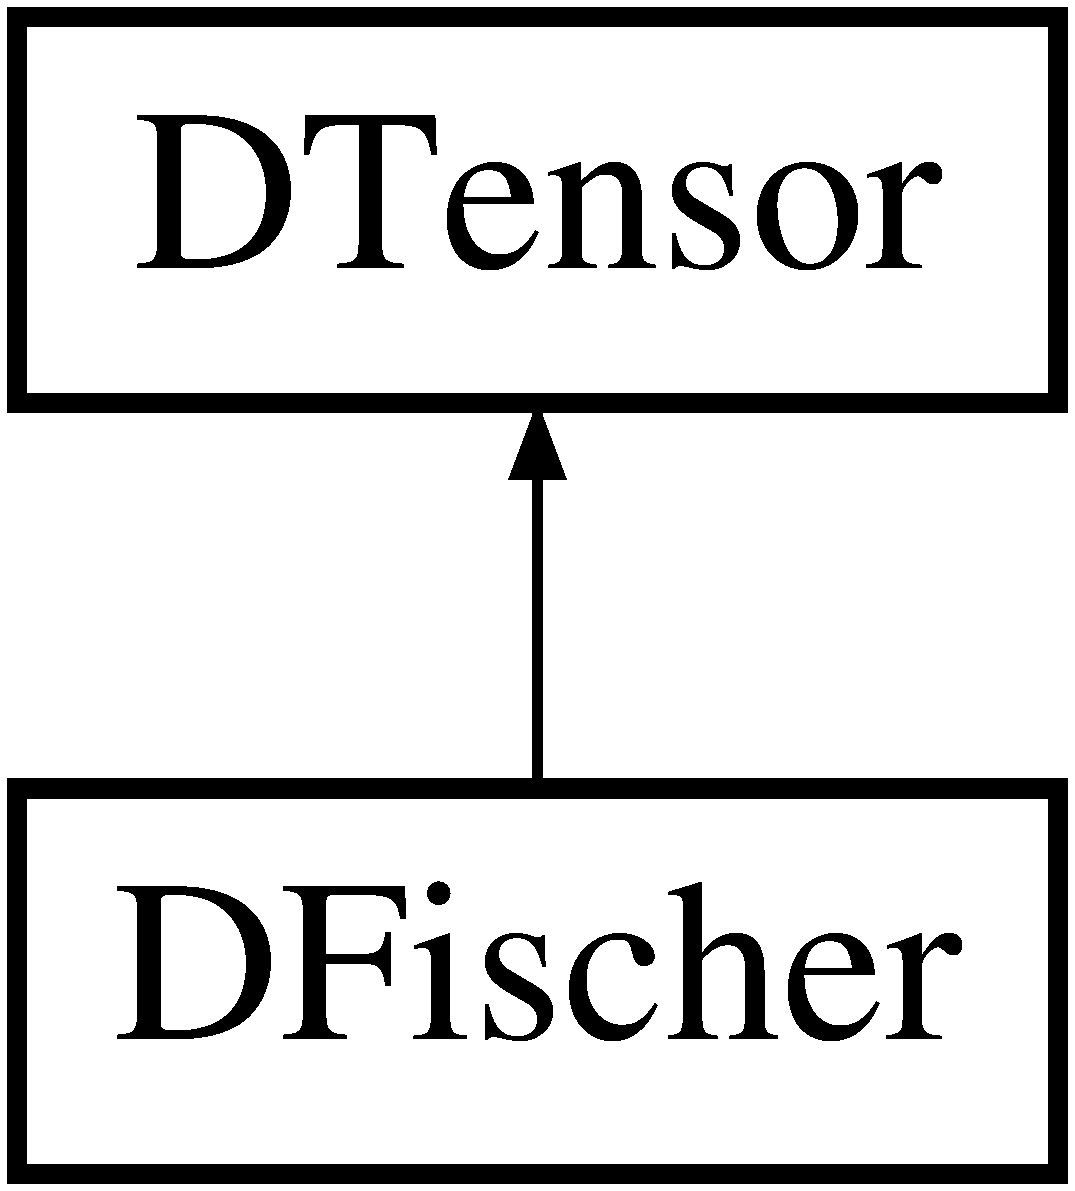
\includegraphics[height=2.000000cm]{class_d_fischer}
\end{center}
\end{figure}
\subsection*{Metody publiczne}
\begin{DoxyCompactItemize}
\item 
\hyperlink{class_d_fischer_ae902c6bcee1e0697298aa0ce16063f06}{D\+Fischer} ()
\begin{DoxyCompactList}\small\item\em Konstruktor. \end{DoxyCompactList}\item 
void \hyperlink{class_d_fischer_a683862f1095c7b1c7331621d79360e40}{Compute\+Tensor} (double Dl, double Dt, \hyperlink{class_point}{Point} \&p)
\end{DoxyCompactItemize}


\subsection{Opis szczegółowy}
Klasa tensora dyspersji. 

Zawiera metody potrzebane do obliczenia wratosci wspolczynnikow tensora dyspersji, wg Fischer et al 1979 \char`\"{}\+Mixing in inland and coastal waters\char`\"{}. 

Definicja w linii 51 pliku tensor.\+h.



\subsection{Dokumentacja konstruktora i destruktora}
\hypertarget{class_d_fischer_ae902c6bcee1e0697298aa0ce16063f06}{}\index{D\+Fischer@{D\+Fischer}!D\+Fischer@{D\+Fischer}}
\index{D\+Fischer@{D\+Fischer}!D\+Fischer@{D\+Fischer}}
\subsubsection[{D\+Fischer}]{\setlength{\rightskip}{0pt plus 5cm}D\+Fischer\+::\+D\+Fischer (
\begin{DoxyParamCaption}
{}
\end{DoxyParamCaption}
)\hspace{0.3cm}{\ttfamily [inline]}}\label{class_d_fischer_ae902c6bcee1e0697298aa0ce16063f06}


Konstruktor. 

Tworzy obiekt Tensora Dyspersji wyznaczanego metoda Fischera 

Definicja w linii 58 pliku tensor.\+h.



\subsection{Dokumentacja funkcji składowych}
\hypertarget{class_d_fischer_a683862f1095c7b1c7331621d79360e40}{}\index{D\+Fischer@{D\+Fischer}!Compute\+Tensor@{Compute\+Tensor}}
\index{Compute\+Tensor@{Compute\+Tensor}!D\+Fischer@{D\+Fischer}}
\subsubsection[{Compute\+Tensor}]{\setlength{\rightskip}{0pt plus 5cm}void D\+Fischer\+::\+Compute\+Tensor (
\begin{DoxyParamCaption}
\item[{double}]{Dl, }
\item[{double}]{Dt, }
\item[{{\bf Point} \&}]{p}
\end{DoxyParamCaption}
)\hspace{0.3cm}{\ttfamily [virtual]}}\label{class_d_fischer_a683862f1095c7b1c7331621d79360e40}
Oblicza wspolczyniki tensora Dyspersji uzywjac odpowieniej metody w zaleznosci od opcji podanej w pliku wejsciowym 
\begin{DoxyParams}{Parametry}
{\em Dl} & -\/ wspolczyniki dyspersji podluznej \\
\hline
{\em Dt} & -\/ wspolczynnik dyspersji porzecznej \\
\hline
{\em p} & -\/ punkt dla ktorego obiczany jest tensor \\
\hline
\end{DoxyParams}


Reimplementowana z \hyperlink{class_d_tensor_a0ed66ce3f3ab159c4d7f6a019bfea9da}{D\+Tensor}.



Definicja w linii 18 pliku tensor.\+cpp.



Dokumentacja dla tej klasy została wygenerowana z plików\+:\begin{DoxyCompactItemize}
\item 
\hyperlink{tensor_8h}{tensor.\+h}\item 
\hyperlink{tensor_8cpp}{tensor.\+cpp}\end{DoxyCompactItemize}

\hypertarget{class_d_fischer2}{}\section{Dokumentacja klasy D\+Fischer2}
\label{class_d_fischer2}\index{D\+Fischer2@{D\+Fischer2}}


Klasa tensora dyspersji.  




{\ttfamily \#include $<$tensor.\+h$>$}

Diagram dziedziczenia dla D\+Fischer2\begin{figure}[H]
\begin{center}
\leavevmode
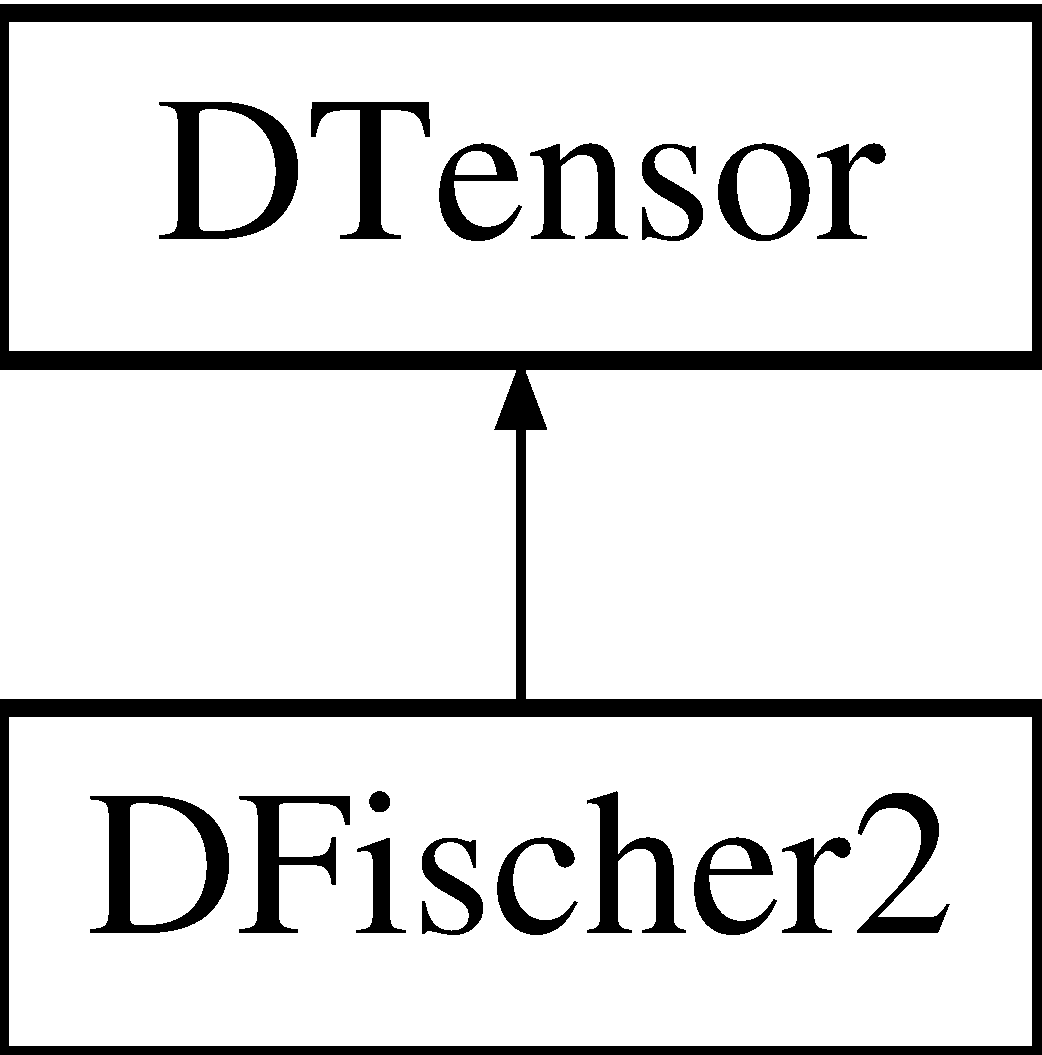
\includegraphics[height=2.000000cm]{class_d_fischer2}
\end{center}
\end{figure}
\subsection*{Metody publiczne}
\begin{DoxyCompactItemize}
\item 
\hyperlink{class_d_fischer2_afa71f15373ca57859ab3f09ec3306bde}{D\+Fischer2} ()
\begin{DoxyCompactList}\small\item\em Konstruktor. \end{DoxyCompactList}\item 
void \hyperlink{class_d_fischer2_ae9c984ac693b39d8ea947aaa975cb0d7}{Compute\+Tensor} (double Dl, double Dt, \hyperlink{class_point}{Point} \&p)
\end{DoxyCompactItemize}


\subsection{Opis szczegółowy}
Klasa tensora dyspersji. 

Zawiera metody potrzebane do obliczenia wratosci wspolczynnikow tensora dyspersji, wg Fischer et al 1979 \char`\"{}\+Mixing in inland and coastal waters\char`\"{}, ale zaniedbujaca pozadiagonalne wspolczynniki. 

Definicja w linii 69 pliku tensor.\+h.



\subsection{Dokumentacja konstruktora i destruktora}
\hypertarget{class_d_fischer2_afa71f15373ca57859ab3f09ec3306bde}{}\index{D\+Fischer2@{D\+Fischer2}!D\+Fischer2@{D\+Fischer2}}
\index{D\+Fischer2@{D\+Fischer2}!D\+Fischer2@{D\+Fischer2}}
\subsubsection[{D\+Fischer2}]{\setlength{\rightskip}{0pt plus 5cm}D\+Fischer2\+::\+D\+Fischer2 (
\begin{DoxyParamCaption}
{}
\end{DoxyParamCaption}
)\hspace{0.3cm}{\ttfamily [inline]}}\label{class_d_fischer2_afa71f15373ca57859ab3f09ec3306bde}


Konstruktor. 

Tworzy obiekt Tensora Dyspersji wyznaczanego metoda Fischera z zaniedbaniem wspolczynnikow pozadiagonalnych 

Definicja w linii 76 pliku tensor.\+h.



\subsection{Dokumentacja funkcji składowych}
\hypertarget{class_d_fischer2_ae9c984ac693b39d8ea947aaa975cb0d7}{}\index{D\+Fischer2@{D\+Fischer2}!Compute\+Tensor@{Compute\+Tensor}}
\index{Compute\+Tensor@{Compute\+Tensor}!D\+Fischer2@{D\+Fischer2}}
\subsubsection[{Compute\+Tensor}]{\setlength{\rightskip}{0pt plus 5cm}void D\+Fischer2\+::\+Compute\+Tensor (
\begin{DoxyParamCaption}
\item[{double}]{Dl, }
\item[{double}]{Dt, }
\item[{{\bf Point} \&}]{p}
\end{DoxyParamCaption}
)\hspace{0.3cm}{\ttfamily [virtual]}}\label{class_d_fischer2_ae9c984ac693b39d8ea947aaa975cb0d7}
Oblicza wspolczyniki tensora Dyspersji uzywjac odpowieniej metody w zaleznosci od opcji podanej w pliku wejsciowym 
\begin{DoxyParams}{Parametry}
{\em Dl} & -\/ wspolczyniki dyspersji podluznej \\
\hline
{\em Dt} & -\/ wspolczynnik dyspersji porzecznej \\
\hline
{\em p} & -\/ punkt dla ktorego obiczany jest tensor \\
\hline
\end{DoxyParams}


Reimplementowana z \hyperlink{class_d_tensor_a0ed66ce3f3ab159c4d7f6a019bfea9da}{D\+Tensor}.



Definicja w linii 50 pliku tensor.\+cpp.



Dokumentacja dla tej klasy została wygenerowana z plików\+:\begin{DoxyCompactItemize}
\item 
\hyperlink{tensor_8h}{tensor.\+h}\item 
\hyperlink{tensor_8cpp}{tensor.\+cpp}\end{DoxyCompactItemize}

\hypertarget{class_d_tensor}{}\section{Dokumentacja klasy D\+Tensor}
\label{class_d_tensor}\index{D\+Tensor@{D\+Tensor}}


Klasa podstawowa tensora dyspersji.  




{\ttfamily \#include $<$tensor.\+h$>$}

Diagram dziedziczenia dla D\+Tensor\begin{figure}[H]
\begin{center}
\leavevmode
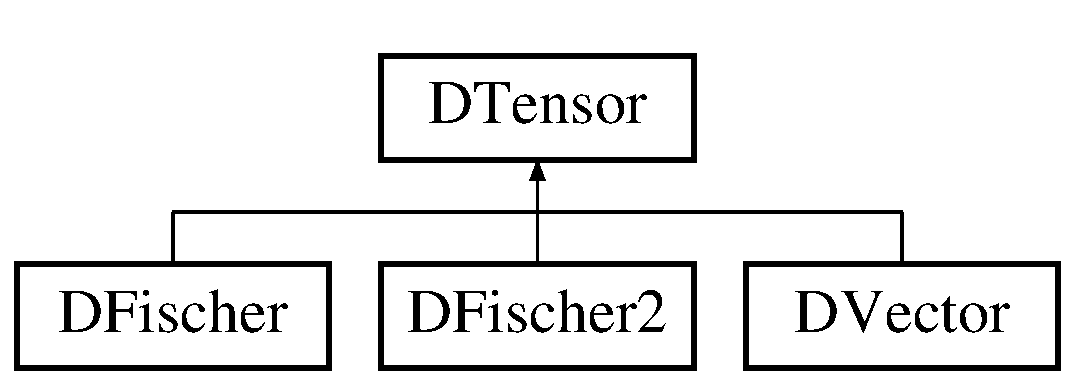
\includegraphics[height=2.000000cm]{class_d_tensor}
\end{center}
\end{figure}
\subsection*{Metody publiczne}
\begin{DoxyCompactItemize}
\item 
\hyperlink{class_d_tensor_ae52ee454318be2245042568f16d5688a}{D\+Tensor} ()
\begin{DoxyCompactList}\small\item\em Konstruktor. \end{DoxyCompactList}\item 
void \hyperlink{class_d_tensor_a341090bb4a7fe3fcb8d21ef27aa84d88}{test} (double Dl, double Dt, \hyperlink{class_point}{Point} \&p)
\item 
virtual void \hyperlink{class_d_tensor_a0ed66ce3f3ab159c4d7f6a019bfea9da}{Compute\+Tensor} (double Dl, double Dt, \hyperlink{class_point}{Point} \&p)
\end{DoxyCompactItemize}


\subsection{Opis szczegółowy}
Klasa podstawowa tensora dyspersji. 

Zawiera metody potrzebane do wyznaczenia wratosci wspolczynnikow tensora dyspersji, w zaleznosci od wybranego sposobu obliczen jest uzywna ona lub jedna z klas pochodnych. 

Definicja w linii 25 pliku tensor.\+h.



\subsection{Dokumentacja konstruktora i destruktora}
\hypertarget{class_d_tensor_ae52ee454318be2245042568f16d5688a}{}\index{D\+Tensor@{D\+Tensor}!D\+Tensor@{D\+Tensor}}
\index{D\+Tensor@{D\+Tensor}!D\+Tensor@{D\+Tensor}}
\subsubsection[{D\+Tensor}]{\setlength{\rightskip}{0pt plus 5cm}D\+Tensor\+::\+D\+Tensor (
\begin{DoxyParamCaption}
{}
\end{DoxyParamCaption}
)\hspace{0.3cm}{\ttfamily [inline]}}\label{class_d_tensor_ae52ee454318be2245042568f16d5688a}


Konstruktor. 

Tworzy obiekt Tensora Dyspersji 

Definicja w linii 32 pliku tensor.\+h.



\subsection{Dokumentacja funkcji składowych}
\hypertarget{class_d_tensor_a0ed66ce3f3ab159c4d7f6a019bfea9da}{}\index{D\+Tensor@{D\+Tensor}!Compute\+Tensor@{Compute\+Tensor}}
\index{Compute\+Tensor@{Compute\+Tensor}!D\+Tensor@{D\+Tensor}}
\subsubsection[{Compute\+Tensor}]{\setlength{\rightskip}{0pt plus 5cm}void D\+Tensor\+::\+Compute\+Tensor (
\begin{DoxyParamCaption}
\item[{double}]{Dl, }
\item[{double}]{Dt, }
\item[{{\bf Point} \&}]{p}
\end{DoxyParamCaption}
)\hspace{0.3cm}{\ttfamily [virtual]}}\label{class_d_tensor_a0ed66ce3f3ab159c4d7f6a019bfea9da}
Oblicza wspolczyniki tensora Dyspersji uzywjac odpowieniej metody w zaleznosci od opcji podanej w pliku wejsciowym 
\begin{DoxyParams}{Parametry}
{\em Dl} & -\/ wspolczyniki dyspersji podluznej \\
\hline
{\em Dt} & -\/ wspolczynnik dyspersji porzecznej \\
\hline
{\em p} & -\/ punkt dla ktorego obiczany jest tensor \\
\hline
\end{DoxyParams}


Reimplementowana w \hyperlink{class_d_vector_a2069ef34d3db2a9965f07e27f17e12dd}{D\+Vector}, \hyperlink{class_d_fischer2_ae9c984ac693b39d8ea947aaa975cb0d7}{D\+Fischer2} i \hyperlink{class_d_fischer_a683862f1095c7b1c7331621d79360e40}{D\+Fischer}.



Definicja w linii 11 pliku tensor.\+cpp.

\hypertarget{class_d_tensor_a341090bb4a7fe3fcb8d21ef27aa84d88}{}\index{D\+Tensor@{D\+Tensor}!test@{test}}
\index{test@{test}!D\+Tensor@{D\+Tensor}}
\subsubsection[{test}]{\setlength{\rightskip}{0pt plus 5cm}void D\+Tensor\+::test (
\begin{DoxyParamCaption}
\item[{double}]{Dl, }
\item[{double}]{Dt, }
\item[{{\bf Point} \&}]{p}
\end{DoxyParamCaption}
)\hspace{0.3cm}{\ttfamily [inline]}}\label{class_d_tensor_a341090bb4a7fe3fcb8d21ef27aa84d88}


Definicja w linii 34 pliku tensor.\+h.



Dokumentacja dla tej klasy została wygenerowana z plików\+:\begin{DoxyCompactItemize}
\item 
\hyperlink{tensor_8h}{tensor.\+h}\item 
\hyperlink{tensor_8cpp}{tensor.\+cpp}\end{DoxyCompactItemize}

\hypertarget{class_d_vector}{}\section{Dokumentacja klasy D\+Vector}
\label{class_d_vector}\index{D\+Vector@{D\+Vector}}


Klasa tensora dyspersji.  




{\ttfamily \#include $<$tensor.\+h$>$}

Diagram dziedziczenia dla D\+Vector\begin{figure}[H]
\begin{center}
\leavevmode
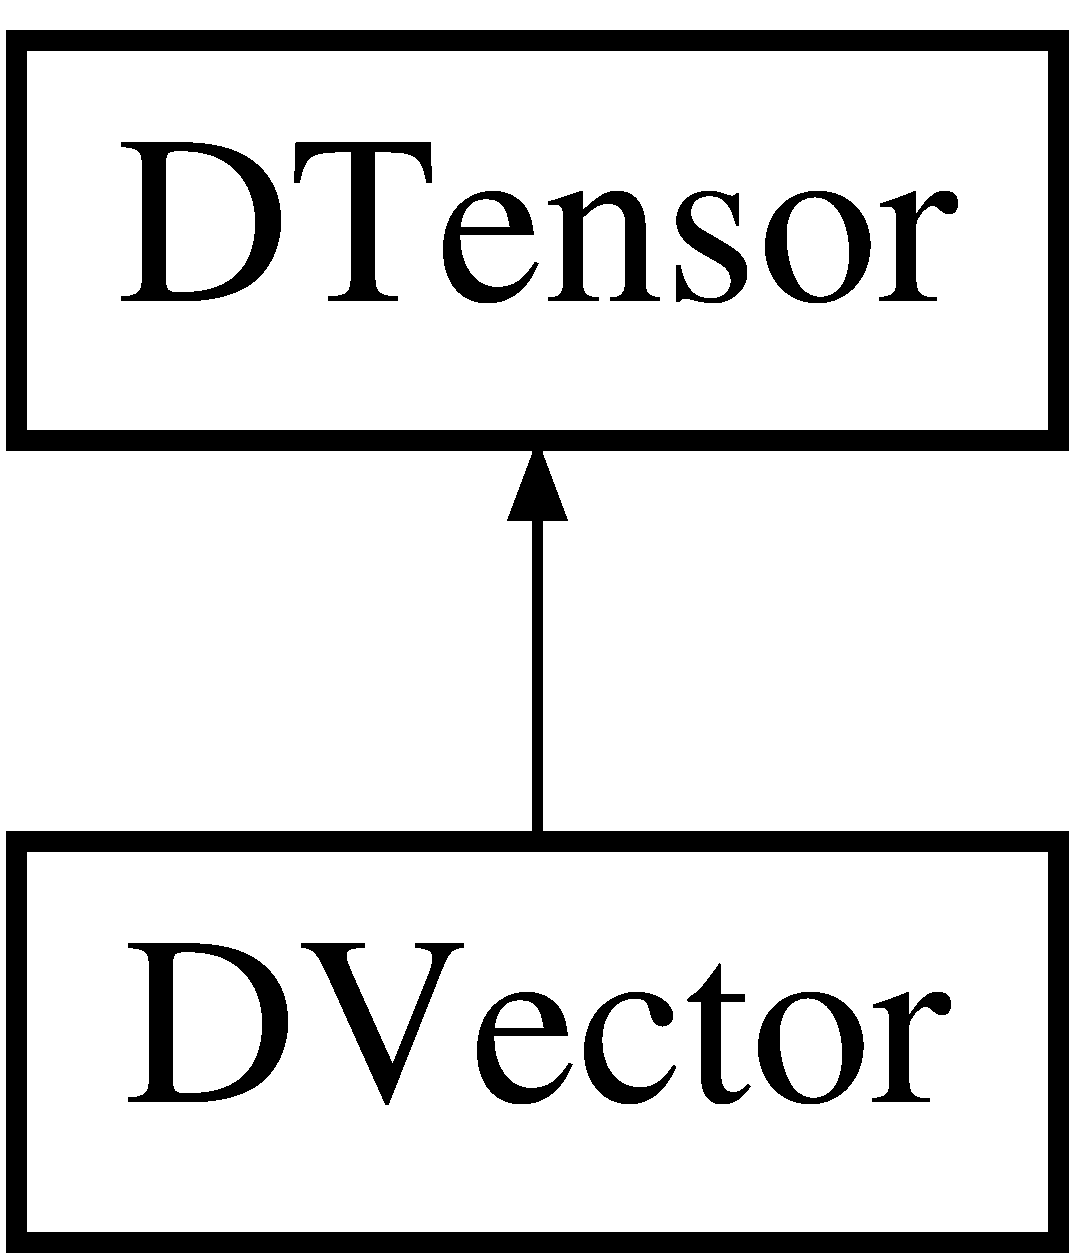
\includegraphics[height=2.000000cm]{class_d_vector}
\end{center}
\end{figure}
\subsection*{Metody publiczne}
\begin{DoxyCompactItemize}
\item 
\hyperlink{class_d_vector_a8acb7f030a2049c718f79d265da12e62}{D\+Vector} ()
\begin{DoxyCompactList}\small\item\em Konstruktor. \end{DoxyCompactList}\item 
void \hyperlink{class_d_vector_a2069ef34d3db2a9965f07e27f17e12dd}{Compute\+Tensor} (double Dl, double Dt, \hyperlink{class_point}{Point} \&p)
\end{DoxyCompactItemize}


\subsection{Opis szczegółowy}
Klasa tensora dyspersji. 

Zawiera metody potrzebane do obliczenia wratosci wspolczynnikow tensora dyspersji, traktujac tensor jako wektor w ukaladzie wspolrzednych \mbox{[}Dl,Dt\mbox{]} i obracajac go do wektora \mbox{[}Dxx, Dyy\mbox{]}. 

Definicja w linii 88 pliku tensor.\+h.



\subsection{Dokumentacja konstruktora i destruktora}
\hypertarget{class_d_vector_a8acb7f030a2049c718f79d265da12e62}{}\index{D\+Vector@{D\+Vector}!D\+Vector@{D\+Vector}}
\index{D\+Vector@{D\+Vector}!D\+Vector@{D\+Vector}}
\subsubsection[{D\+Vector}]{\setlength{\rightskip}{0pt plus 5cm}D\+Vector\+::\+D\+Vector (
\begin{DoxyParamCaption}
{}
\end{DoxyParamCaption}
)\hspace{0.3cm}{\ttfamily [inline]}}\label{class_d_vector_a8acb7f030a2049c718f79d265da12e62}


Konstruktor. 

Tworzy obiekt Tensora Dyspersji traktowanego jako wektor 

Definicja w linii 95 pliku tensor.\+h.



\subsection{Dokumentacja funkcji składowych}
\hypertarget{class_d_vector_a2069ef34d3db2a9965f07e27f17e12dd}{}\index{D\+Vector@{D\+Vector}!Compute\+Tensor@{Compute\+Tensor}}
\index{Compute\+Tensor@{Compute\+Tensor}!D\+Vector@{D\+Vector}}
\subsubsection[{Compute\+Tensor}]{\setlength{\rightskip}{0pt plus 5cm}void D\+Vector\+::\+Compute\+Tensor (
\begin{DoxyParamCaption}
\item[{double}]{Dl, }
\item[{double}]{Dt, }
\item[{{\bf Point} \&}]{p}
\end{DoxyParamCaption}
)\hspace{0.3cm}{\ttfamily [virtual]}}\label{class_d_vector_a2069ef34d3db2a9965f07e27f17e12dd}
Oblicza wspolczyniki tensora Dyspersji uzywjac odpowieniej metody w zaleznosci od opcji podanej w pliku wejsciowym 
\begin{DoxyParams}{Parametry}
{\em Dl} & -\/ wspolczyniki dyspersji podluznej \\
\hline
{\em Dt} & -\/ wspolczynnik dyspersji porzecznej \\
\hline
{\em p} & -\/ punkt dla ktorego obiczany jest tensor \\
\hline
\end{DoxyParams}


Reimplementowana z \hyperlink{class_d_tensor_a0ed66ce3f3ab159c4d7f6a019bfea9da}{D\+Tensor}.



Definicja w linii 82 pliku tensor.\+cpp.



Dokumentacja dla tej klasy została wygenerowana z plików\+:\begin{DoxyCompactItemize}
\item 
\hyperlink{tensor_8h}{tensor.\+h}\item 
\hyperlink{tensor_8cpp}{tensor.\+cpp}\end{DoxyCompactItemize}

\hypertarget{class_grid}{}\section{Dokumentacja klasy Grid}
\label{class_grid}\index{Grid@{Grid}}


Klasa Przygotowujaca siatke do symulacji.  




{\ttfamily \#include $<$grid.\+h$>$}

Diagram dziedziczenia dla Grid\begin{figure}[H]
\begin{center}
\leavevmode
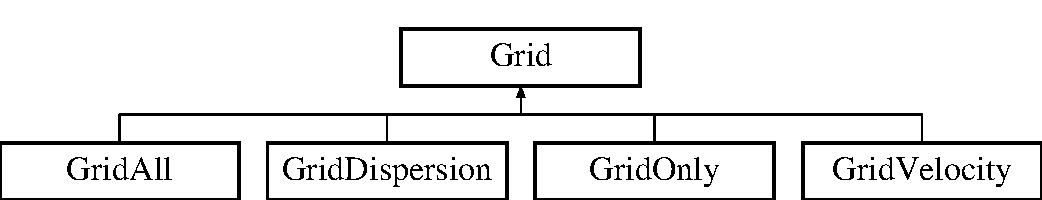
\includegraphics[height=2.000000cm]{class_grid}
\end{center}
\end{figure}
\subsection*{Metody publiczne}
\begin{DoxyCompactItemize}
\item 
virtual int \hyperlink{class_grid_ac0cf78c28206fd44fba21c5a91d0a0e0}{Read\+Data} (map$<$ int, \hyperlink{class_point}{Point} $>$ \&Point\+Map, const string \&file, \hyperlink{class_simulation_parameters}{Simulation\+Parameters} \&sym\+\_\+param)
\item 
void \hyperlink{class_grid_affe0d058372cb86ef7816d536793341b}{Set\+Max\+Values} (double \&vx, double \&vy, double \&Dxx, double \&Dxy, double Dyy, \hyperlink{class_simulation_parameters}{Simulation\+Parameters} \&param)
\item 
void \hyperlink{class_grid_a25ecf93fd041648dcde213623589fa27}{Set\+Min\+Values} (double \&vx, double \&vy, double \&Dxx, double \&Dxy, double Dyy, \hyperlink{class_simulation_parameters}{Simulation\+Parameters} \&param)
\item 
void \hyperlink{class_grid_a4fc635f29b3dfa2075dc7e3cc6861762}{Set\+Extreme\+Values} (double \&xmax, double \&xmin, double \&ymax, double \&ymin)
\item 
void \hyperlink{class_grid_a03696ec5383f1a0222b447a0ff15d47c}{Set\+Extreme\+Points} (\hyperlink{class_point}{Point} \&pxmax, \hyperlink{class_point}{Point} \&pxmin, \hyperlink{class_point}{Point} \&pymax, \hyperlink{class_point}{Point} \&pymin)
\item 
void \hyperlink{class_grid_a3070db37370246f2028310f412d3d8c3}{Complete\+Outside\+Flow} (map$<$ int, \hyperlink{class_point}{Point} $>$ \&Point\+Map)
\item 
int \hyperlink{class_grid_ac438ff968a29cfaaebb410f2a08a48f4}{Correct\+Grid} (map$<$ int, \hyperlink{class_point}{Point} $>$ \&Point\+Map)
\item 
void \hyperlink{class_grid_a1e040eda61d389f8e0d141933ed6fb48}{Mark\+Border\+Points} (map$<$ int, \hyperlink{class_point}{Point} $>$ \&Point\+Map)
\item 
void \hyperlink{class_grid_a6270d5bfcdefee9477865a3a60baae73}{Mark\+Near\+Border\+Points} (map$<$ int, \hyperlink{class_point}{Point} $>$ \&Point\+Map)
\item 
int \hyperlink{class_grid_a0cc5771c532b0a92abb64d7f2df8eb1f}{Mark\+In\+Out\+Points} (map$<$ int, \hyperlink{class_point}{Point} $>$ \&Point\+Map)
\item 
void \hyperlink{class_grid_acdec1d78fe3ead312d1098837325d113}{set\+\_\+pxmax} (\hyperlink{class_point}{Point} pkt)
\item 
void \hyperlink{class_grid_a51aaeb13d9c299ebc07e1e9d3b9fe47f}{set\+\_\+pymax} (\hyperlink{class_point}{Point} pkt)
\item 
void \hyperlink{class_grid_ab01ea11cdb5d87a4d8cddb51b40dd52c}{set\+\_\+pxmin} (\hyperlink{class_point}{Point} pkt)
\item 
void \hyperlink{class_grid_a666541ca159aebd16470f1fa7b2d16c2}{set\+\_\+pymin} (\hyperlink{class_point}{Point} pkt)
\item 
\hyperlink{class_point}{Point} \hyperlink{class_grid_ae90bb3028aa13b363d61e6617f4dbd89}{get\+\_\+pxmax} () const 
\item 
\hyperlink{class_point}{Point} \hyperlink{class_grid_ab45d29e63d5a92a97d2a8bc034e96234}{get\+\_\+pymax} () const 
\item 
\hyperlink{class_point}{Point} \hyperlink{class_grid_aa52105935ef29936395898215bcf40a7}{get\+\_\+pxmin} () const 
\item 
\hyperlink{class_point}{Point} \hyperlink{class_grid_a9865c790dde45934add338c055247a4c}{get\+\_\+pymin} () const 
\item 
double \hyperlink{class_grid_a2646150f8d14820de6c40a296d2eba17}{get\+\_\+xmax} () const 
\item 
double \hyperlink{class_grid_a385b11b22ff42896d522400d9ddd7e97}{get\+\_\+ymax} () const 
\item 
double \hyperlink{class_grid_a1ff74bf0898894452d67ccda6e3dc266}{get\+\_\+xmin} () const 
\item 
double \hyperlink{class_grid_ae776aec819443b168ebe15a52632ad77}{get\+\_\+ymin} () const 
\end{DoxyCompactItemize}
\subsection*{Statyczne atrybuty publiczne}
\begin{DoxyCompactItemize}
\item 
static const int \hyperlink{class_grid_a557878ff6ca7473b0a0acb3ae9c599cb}{empty\+\_\+index} = -\/99999999
\item 
static int \hyperlink{class_grid_a1f0576a19198685cba8f1067b7e1ba7c}{\+\_\+xmax} = 0
\item 
static int \hyperlink{class_grid_a293bb2eb514f57749e92d2dcf914ca57}{\+\_\+xmin} = 0
\item 
static int \hyperlink{class_grid_ab4c6a5500c2540b48194a7bcdefab235}{\+\_\+ymax} = 0
\item 
static int \hyperlink{class_grid_a6e548ba7ad924ef369c7fc24be04f0b2}{\+\_\+ymin} = 0
\end{DoxyCompactItemize}


\subsection{Opis szczegółowy}
Klasa Przygotowujaca siatke do symulacji. 

Zawiera funkcje potrzebne do przgotowania siatki, wspolne dla roznych sposobow wczytywania danych. 

Definicja w linii 26 pliku grid.\+h.



\subsection{Dokumentacja funkcji składowych}
\hypertarget{class_grid_a3070db37370246f2028310f412d3d8c3}{}\index{Grid@{Grid}!Complete\+Outside\+Flow@{Complete\+Outside\+Flow}}
\index{Complete\+Outside\+Flow@{Complete\+Outside\+Flow}!Grid@{Grid}}
\subsubsection[{Complete\+Outside\+Flow}]{\setlength{\rightskip}{0pt plus 5cm}void Grid\+::\+Complete\+Outside\+Flow (
\begin{DoxyParamCaption}
\item[{map$<$ int, {\bf Point} $>$ \&}]{Point\+Map}
\end{DoxyParamCaption}
)}\label{class_grid_a3070db37370246f2028310f412d3d8c3}
Korzystajac z wyznaczony wartosci namniejszych i najwiekszych wspolrzednych na siatce, uzuplnia siatke punktami, ktore leza poza przeplywem nadajac im flage 0 
\begin{DoxyParams}{Parametry}
{\em Point\+Map} & -\/ referencja do Mapy Punktow \\
\hline
\end{DoxyParams}


Definicja w linii 65 pliku grid.\+cpp.

\hypertarget{class_grid_ac438ff968a29cfaaebb410f2a08a48f4}{}\index{Grid@{Grid}!Correct\+Grid@{Correct\+Grid}}
\index{Correct\+Grid@{Correct\+Grid}!Grid@{Grid}}
\subsubsection[{Correct\+Grid}]{\setlength{\rightskip}{0pt plus 5cm}int Grid\+::\+Correct\+Grid (
\begin{DoxyParamCaption}
\item[{map$<$ int, {\bf Point} $>$ \&}]{Point\+Map}
\end{DoxyParamCaption}
)}\label{class_grid_ac438ff968a29cfaaebb410f2a08a48f4}
Po oznaczeniu najblizszych sasiadow kazdego pktu koryguje siatkę (korzysta z flag pkt onaczonych jako przeplyw i poz przeplywem); Ustawia flagi 0 (poza przepływem) dla \char`\"{}dziwnych\char`\"{} punktow dla których punkty obok są poza przepływem (nie ma sensu liczyc w tych punktach -\/ generowaloby to tylko bledy nyumeryczne)\+: 
\begin{DoxyParams}{Parametry}
{\em Point\+Map} & -\/ referencja do Mapy Punktow \\
\hline
\end{DoxyParams}


Definicja w linii 84 pliku grid.\+cpp.

\hypertarget{class_grid_ae90bb3028aa13b363d61e6617f4dbd89}{}\index{Grid@{Grid}!get\+\_\+pxmax@{get\+\_\+pxmax}}
\index{get\+\_\+pxmax@{get\+\_\+pxmax}!Grid@{Grid}}
\subsubsection[{get\+\_\+pxmax}]{\setlength{\rightskip}{0pt plus 5cm}{\bf Point} Grid\+::get\+\_\+pxmax (
\begin{DoxyParamCaption}
{}
\end{DoxyParamCaption}
) const\hspace{0.3cm}{\ttfamily [inline]}}\label{class_grid_ae90bb3028aa13b363d61e6617f4dbd89}
Zwaraca pkt majacy maksymalna wartosc wspolrzednej x na siatce 

Definicja w linii 159 pliku grid.\+h.

\hypertarget{class_grid_aa52105935ef29936395898215bcf40a7}{}\index{Grid@{Grid}!get\+\_\+pxmin@{get\+\_\+pxmin}}
\index{get\+\_\+pxmin@{get\+\_\+pxmin}!Grid@{Grid}}
\subsubsection[{get\+\_\+pxmin}]{\setlength{\rightskip}{0pt plus 5cm}{\bf Point} Grid\+::get\+\_\+pxmin (
\begin{DoxyParamCaption}
{}
\end{DoxyParamCaption}
) const\hspace{0.3cm}{\ttfamily [inline]}}\label{class_grid_aa52105935ef29936395898215bcf40a7}
Zwaraca pkt majacy minimalna wartosc wspolzrednej x na siatce 

Definicja w linii 165 pliku grid.\+h.

\hypertarget{class_grid_ab45d29e63d5a92a97d2a8bc034e96234}{}\index{Grid@{Grid}!get\+\_\+pymax@{get\+\_\+pymax}}
\index{get\+\_\+pymax@{get\+\_\+pymax}!Grid@{Grid}}
\subsubsection[{get\+\_\+pymax}]{\setlength{\rightskip}{0pt plus 5cm}{\bf Point} Grid\+::get\+\_\+pymax (
\begin{DoxyParamCaption}
{}
\end{DoxyParamCaption}
) const\hspace{0.3cm}{\ttfamily [inline]}}\label{class_grid_ab45d29e63d5a92a97d2a8bc034e96234}
Zwaraca pkt majacy maksymalna wartosc wspolrzednej y na siatce 

Definicja w linii 162 pliku grid.\+h.

\hypertarget{class_grid_a9865c790dde45934add338c055247a4c}{}\index{Grid@{Grid}!get\+\_\+pymin@{get\+\_\+pymin}}
\index{get\+\_\+pymin@{get\+\_\+pymin}!Grid@{Grid}}
\subsubsection[{get\+\_\+pymin}]{\setlength{\rightskip}{0pt plus 5cm}{\bf Point} Grid\+::get\+\_\+pymin (
\begin{DoxyParamCaption}
{}
\end{DoxyParamCaption}
) const\hspace{0.3cm}{\ttfamily [inline]}}\label{class_grid_a9865c790dde45934add338c055247a4c}
Zwaraca pkt majacy minimalna wartosc wpolrzednej y na siatce 

Definicja w linii 168 pliku grid.\+h.

\hypertarget{class_grid_a2646150f8d14820de6c40a296d2eba17}{}\index{Grid@{Grid}!get\+\_\+xmax@{get\+\_\+xmax}}
\index{get\+\_\+xmax@{get\+\_\+xmax}!Grid@{Grid}}
\subsubsection[{get\+\_\+xmax}]{\setlength{\rightskip}{0pt plus 5cm}double Grid\+::get\+\_\+xmax (
\begin{DoxyParamCaption}
{}
\end{DoxyParamCaption}
) const\hspace{0.3cm}{\ttfamily [inline]}}\label{class_grid_a2646150f8d14820de6c40a296d2eba17}
Zwaraca maksymalna wartosc wspolrzednej x na siatce 

Definicja w linii 172 pliku grid.\+h.

\hypertarget{class_grid_a1ff74bf0898894452d67ccda6e3dc266}{}\index{Grid@{Grid}!get\+\_\+xmin@{get\+\_\+xmin}}
\index{get\+\_\+xmin@{get\+\_\+xmin}!Grid@{Grid}}
\subsubsection[{get\+\_\+xmin}]{\setlength{\rightskip}{0pt plus 5cm}double Grid\+::get\+\_\+xmin (
\begin{DoxyParamCaption}
{}
\end{DoxyParamCaption}
) const\hspace{0.3cm}{\ttfamily [inline]}}\label{class_grid_a1ff74bf0898894452d67ccda6e3dc266}
Zwaraca minimalna wartosc wspolzrednej x na siatce 

Definicja w linii 178 pliku grid.\+h.

\hypertarget{class_grid_a385b11b22ff42896d522400d9ddd7e97}{}\index{Grid@{Grid}!get\+\_\+ymax@{get\+\_\+ymax}}
\index{get\+\_\+ymax@{get\+\_\+ymax}!Grid@{Grid}}
\subsubsection[{get\+\_\+ymax}]{\setlength{\rightskip}{0pt plus 5cm}double Grid\+::get\+\_\+ymax (
\begin{DoxyParamCaption}
{}
\end{DoxyParamCaption}
) const\hspace{0.3cm}{\ttfamily [inline]}}\label{class_grid_a385b11b22ff42896d522400d9ddd7e97}
Zwaraca maksymalna wartosc wspolrzednej y na siatce 

Definicja w linii 175 pliku grid.\+h.

\hypertarget{class_grid_ae776aec819443b168ebe15a52632ad77}{}\index{Grid@{Grid}!get\+\_\+ymin@{get\+\_\+ymin}}
\index{get\+\_\+ymin@{get\+\_\+ymin}!Grid@{Grid}}
\subsubsection[{get\+\_\+ymin}]{\setlength{\rightskip}{0pt plus 5cm}double Grid\+::get\+\_\+ymin (
\begin{DoxyParamCaption}
{}
\end{DoxyParamCaption}
) const\hspace{0.3cm}{\ttfamily [inline]}}\label{class_grid_ae776aec819443b168ebe15a52632ad77}
Zwaraca minimalna wartosc wpolrzednej y na siatce 

Definicja w linii 181 pliku grid.\+h.

\hypertarget{class_grid_a1e040eda61d389f8e0d141933ed6fb48}{}\index{Grid@{Grid}!Mark\+Border\+Points@{Mark\+Border\+Points}}
\index{Mark\+Border\+Points@{Mark\+Border\+Points}!Grid@{Grid}}
\subsubsection[{Mark\+Border\+Points}]{\setlength{\rightskip}{0pt plus 5cm}void Grid\+::\+Mark\+Border\+Points (
\begin{DoxyParamCaption}
\item[{map$<$ int, {\bf Point} $>$ \&}]{Point\+Map}
\end{DoxyParamCaption}
)}\label{class_grid_a1e040eda61d389f8e0d141933ed6fb48}
Po oznaczeniu najblizszych sasiadow kazdego pktu i ewentulanie korekcji siatki wyznacza brzeg obszaru przeplywu (korzysta z flag pkt onaczonych jako przeplyw i poz przeplywem); Ustawia odpowiednie flagi punktow w zaleznosci od rodzaju brzegu do ktorego pktr nalezy\+: 
\begin{DoxyItemize}
\item brzeg gorny -\/$>$ flaga {\bfseries 2} 
\item brzeg dolny -\/$>$ flaga {\bfseries 3} 
\item brzeg lewy -\/$>$ flaga {\bfseries 4} 
\item brzeg prawy -\/$>$ flaga {\bfseries 5} 
\item rog gorny-\/lewy -\/$>$ flaga {\bfseries 24} 
\item rog gorny-\/prawy -\/$>$ flaga {\bfseries 25} 
\item rog dolny-\/lewy -\/$>$ flaga {\bfseries 34} 
\item rog dolny-\/prawy -\/$>$ flaga {\bfseries 35} 
\item kanty -\/$>$ flaga {\bfseries 1} 
\item zrodla -\/$>$ flaga {\bfseries 101} 
\end{DoxyItemize}
\begin{DoxyParams}{Parametry}
{\em Point\+Map} & -\/ referencja do Mapy Punktow \\
\hline
\end{DoxyParams}


Definicja w linii 174 pliku grid.\+cpp.

\hypertarget{class_grid_a0cc5771c532b0a92abb64d7f2df8eb1f}{}\index{Grid@{Grid}!Mark\+In\+Out\+Points@{Mark\+In\+Out\+Points}}
\index{Mark\+In\+Out\+Points@{Mark\+In\+Out\+Points}!Grid@{Grid}}
\subsubsection[{Mark\+In\+Out\+Points}]{\setlength{\rightskip}{0pt plus 5cm}int Grid\+::\+Mark\+In\+Out\+Points (
\begin{DoxyParamCaption}
\item[{map$<$ int, {\bf Point} $>$ \&}]{Point\+Map}
\end{DoxyParamCaption}
)}\label{class_grid_a0cc5771c532b0a92abb64d7f2df8eb1f}
Ustawia odpowiednie flagi punktow lezacych na wejsciach i wyjsciach; 
\begin{DoxyParams}{Parametry}
{\em Point\+Map} & -\/ referencja do Mapy Punktow\\
\hline
\end{DoxyParams}
{\bfseries D\+O N\+A\+P\+I\+S\+A\+N\+I\+A } na razie prowizorycznie w konkretnym przypadku!!! !! moze pozniej bedzie potrzbne !! 

Definicja w linii 361 pliku grid.\+cpp.

\hypertarget{class_grid_a6270d5bfcdefee9477865a3a60baae73}{}\index{Grid@{Grid}!Mark\+Near\+Border\+Points@{Mark\+Near\+Border\+Points}}
\index{Mark\+Near\+Border\+Points@{Mark\+Near\+Border\+Points}!Grid@{Grid}}
\subsubsection[{Mark\+Near\+Border\+Points}]{\setlength{\rightskip}{0pt plus 5cm}void Grid\+::\+Mark\+Near\+Border\+Points (
\begin{DoxyParamCaption}
\item[{map$<$ int, {\bf Point} $>$ \&}]{Point\+Map}
\end{DoxyParamCaption}
)}\label{class_grid_a6270d5bfcdefee9477865a3a60baae73}
Po oznaczeniu dalszych sasiadow kazdego pktu, Ustawia odpowiednie flagi punktow lezacych przy brzegach; w zaleznosci od rodzaju brzegu do ktorym lezy pkt \+: 
\begin{DoxyItemize}
\item przy brzegu gornym -\/$>$ flaga {\bfseries 22} 
\item przy brzegu dolnym -\/$>$ flaga {\bfseries 33} 
\item przy brzegu lewym -\/$>$ flaga {\bfseries 44} 
\item przy brzegu prawym -\/$>$ flaga {\bfseries 55} 
\item przy rogu gornym-\/lewym -\/$>$ flaga {\bfseries 2244} 
\item przy rogu gornym-\/prawym -\/$>$ flaga {\bfseries 2255} 
\item przy rogu dolnym-\/lewym -\/$>$ flaga {\bfseries 3344} 
\item przy rogu dolnym-\/prawym -\/$>$ flaga {\bfseries 3355} 
\end{DoxyItemize}
\begin{DoxyParams}{Parametry}
{\em Point\+Map} & -\/ referencja do Mapy Punktow \\
\hline
\end{DoxyParams}


Definicja w linii 464 pliku grid.\+cpp.

\hypertarget{class_grid_ac0cf78c28206fd44fba21c5a91d0a0e0}{}\index{Grid@{Grid}!Read\+Data@{Read\+Data}}
\index{Read\+Data@{Read\+Data}!Grid@{Grid}}
\subsubsection[{Read\+Data}]{\setlength{\rightskip}{0pt plus 5cm}virtual int Grid\+::\+Read\+Data (
\begin{DoxyParamCaption}
\item[{map$<$ int, {\bf Point} $>$ \&}]{Point\+Map, }
\item[{const string \&}]{file, }
\item[{{\bf Simulation\+Parameters} \&}]{sym\+\_\+param}
\end{DoxyParamCaption}
)\hspace{0.3cm}{\ttfamily [inline]}, {\ttfamily [virtual]}}\label{class_grid_ac0cf78c28206fd44fba21c5a91d0a0e0}
Wczytywania dane z pliku wejsciowego do mapy punktow 
\begin{DoxyParams}{Parametry}
{\em Point\+Map} & -\/ referencja do Mapy Punktow \\
\hline
{\em file} & -\/ nazwa pliku z danymi \\
\hline
{\em sym\+\_\+param} & -\/ obiekt z parametrami symulacji \\
\hline
\end{DoxyParams}


Reimplementowana w \hyperlink{class_grid_dispersion_afbc03fca9459c90c19959c24df944766}{Grid\+Dispersion}, \hyperlink{class_grid_all_aa513371e605fe9bea7489edfe3d40a1f}{Grid\+All}, \hyperlink{class_grid_velocity_a00143f2982252ae30ceb725886c11ab6}{Grid\+Velocity} i \hyperlink{class_grid_only_a86e143a957ba61c0a5b215b65ea24902}{Grid\+Only}.



Definicja w linii 34 pliku grid.\+h.

\hypertarget{class_grid_acdec1d78fe3ead312d1098837325d113}{}\index{Grid@{Grid}!set\+\_\+pxmax@{set\+\_\+pxmax}}
\index{set\+\_\+pxmax@{set\+\_\+pxmax}!Grid@{Grid}}
\subsubsection[{set\+\_\+pxmax}]{\setlength{\rightskip}{0pt plus 5cm}void Grid\+::set\+\_\+pxmax (
\begin{DoxyParamCaption}
\item[{{\bf Point}}]{pkt}
\end{DoxyParamCaption}
)\hspace{0.3cm}{\ttfamily [inline]}}\label{class_grid_acdec1d78fe3ead312d1098837325d113}
Ustawia pkt z maxymalana wartoscia wspolrzednej x 

Definicja w linii 145 pliku grid.\+h.

\hypertarget{class_grid_ab01ea11cdb5d87a4d8cddb51b40dd52c}{}\index{Grid@{Grid}!set\+\_\+pxmin@{set\+\_\+pxmin}}
\index{set\+\_\+pxmin@{set\+\_\+pxmin}!Grid@{Grid}}
\subsubsection[{set\+\_\+pxmin}]{\setlength{\rightskip}{0pt plus 5cm}void Grid\+::set\+\_\+pxmin (
\begin{DoxyParamCaption}
\item[{{\bf Point}}]{pkt}
\end{DoxyParamCaption}
)\hspace{0.3cm}{\ttfamily [inline]}}\label{class_grid_ab01ea11cdb5d87a4d8cddb51b40dd52c}
Ustawia pkt z minimalan wartoscia wspolrzednej x 

Definicja w linii 151 pliku grid.\+h.

\hypertarget{class_grid_a51aaeb13d9c299ebc07e1e9d3b9fe47f}{}\index{Grid@{Grid}!set\+\_\+pymax@{set\+\_\+pymax}}
\index{set\+\_\+pymax@{set\+\_\+pymax}!Grid@{Grid}}
\subsubsection[{set\+\_\+pymax}]{\setlength{\rightskip}{0pt plus 5cm}void Grid\+::set\+\_\+pymax (
\begin{DoxyParamCaption}
\item[{{\bf Point}}]{pkt}
\end{DoxyParamCaption}
)\hspace{0.3cm}{\ttfamily [inline]}}\label{class_grid_a51aaeb13d9c299ebc07e1e9d3b9fe47f}
Ustawia pkt z maxymalana wartoscia wspolrzednej y 

Definicja w linii 148 pliku grid.\+h.

\hypertarget{class_grid_a666541ca159aebd16470f1fa7b2d16c2}{}\index{Grid@{Grid}!set\+\_\+pymin@{set\+\_\+pymin}}
\index{set\+\_\+pymin@{set\+\_\+pymin}!Grid@{Grid}}
\subsubsection[{set\+\_\+pymin}]{\setlength{\rightskip}{0pt plus 5cm}void Grid\+::set\+\_\+pymin (
\begin{DoxyParamCaption}
\item[{{\bf Point}}]{pkt}
\end{DoxyParamCaption}
)\hspace{0.3cm}{\ttfamily [inline]}}\label{class_grid_a666541ca159aebd16470f1fa7b2d16c2}
Ustawia pkt z minimalna wartoscia wspolrzednej y 

Definicja w linii 154 pliku grid.\+h.

\hypertarget{class_grid_a03696ec5383f1a0222b447a0ff15d47c}{}\index{Grid@{Grid}!Set\+Extreme\+Points@{Set\+Extreme\+Points}}
\index{Set\+Extreme\+Points@{Set\+Extreme\+Points}!Grid@{Grid}}
\subsubsection[{Set\+Extreme\+Points}]{\setlength{\rightskip}{0pt plus 5cm}void Grid\+::\+Set\+Extreme\+Points (
\begin{DoxyParamCaption}
\item[{{\bf Point} \&}]{pxmax, }
\item[{{\bf Point} \&}]{pxmin, }
\item[{{\bf Point} \&}]{pymax, }
\item[{{\bf Point} \&}]{pymin}
\end{DoxyParamCaption}
)}\label{class_grid_a03696ec5383f1a0222b447a0ff15d47c}
Ustawia punkty graniczne siatki 
\begin{DoxyParams}{Parametry}
{\em pxmax} & -\/ refer. do punktu psosiadajacego najwieksza wartosc wspolz. x na siatce \\
\hline
{\em pxmin} & -\/ refer. do punktu psosiadajacego najmniejsza wartosc wspolz. x na siatce \\
\hline
{\em pxmax} & -\/ refer. do punktu psosiadajacego najwieksza wartosc wspolz. y na siatce \\
\hline
{\em pxmax} & -\/ refer. do punktu psosiadajacego najmniejsza wartosc wspolz. y na siatce \\
\hline
\end{DoxyParams}


Definicja w linii 51 pliku grid.\+cpp.

\hypertarget{class_grid_a4fc635f29b3dfa2075dc7e3cc6861762}{}\index{Grid@{Grid}!Set\+Extreme\+Values@{Set\+Extreme\+Values}}
\index{Set\+Extreme\+Values@{Set\+Extreme\+Values}!Grid@{Grid}}
\subsubsection[{Set\+Extreme\+Values}]{\setlength{\rightskip}{0pt plus 5cm}void Grid\+::\+Set\+Extreme\+Values (
\begin{DoxyParamCaption}
\item[{double \&}]{xmax, }
\item[{double \&}]{xmin, }
\item[{double \&}]{ymax, }
\item[{double \&}]{ymin}
\end{DoxyParamCaption}
)}\label{class_grid_a4fc635f29b3dfa2075dc7e3cc6861762}
Ustawia wartosci max i min wspolrzednych x i y na siatce 
\begin{DoxyParams}{Parametry}
{\em xmax} & -\/ refer. do najwiekszej wartosc wspolz. x na siatce \\
\hline
{\em xmin} & -\/ refer. do najmniejszej wartosc wspolz. x na siatce \\
\hline
{\em xmax} & -\/ refer. do najwiekszej wartosc wspolz. y na siatce \\
\hline
{\em xmax} & -\/ refer. do najmniejszej wartosc wspolz. y na siatce \\
\hline
\end{DoxyParams}


Definicja w linii 43 pliku grid.\+cpp.

\hypertarget{class_grid_affe0d058372cb86ef7816d536793341b}{}\index{Grid@{Grid}!Set\+Max\+Values@{Set\+Max\+Values}}
\index{Set\+Max\+Values@{Set\+Max\+Values}!Grid@{Grid}}
\subsubsection[{Set\+Max\+Values}]{\setlength{\rightskip}{0pt plus 5cm}void Grid\+::\+Set\+Max\+Values (
\begin{DoxyParamCaption}
\item[{double \&}]{vx, }
\item[{double \&}]{vy, }
\item[{double \&}]{Dxx, }
\item[{double \&}]{Dxy, }
\item[{double}]{Dyy, }
\item[{{\bf Simulation\+Parameters} \&}]{param}
\end{DoxyParamCaption}
)}\label{class_grid_affe0d058372cb86ef7816d536793341b}
Ustawianie max wartosci zmiennych w parametrcha symulacji 
\begin{DoxyParams}{Parametry}
{\em vx} & -\/ refer. do maksymalnej skladowej x wektora predkosci \\
\hline
{\em vy} & -\/ refer. do maksymalnej skladowej y wektora predkosci \\
\hline
{\em Dxx} & -\/ refer. do maksymalnej skladowej xx tensora Dyspersji \\
\hline
{\em Dxy} & -\/ refer. do maksymalnej skladowej xy tensora Dyspersji \\
\hline
{\em Dyy} & -\/ refer. do maksymalnej skladowej tensora Dyspersji \\
\hline
{\em param} & -\/ referencje do obiektu z parametrami symulacji \\
\hline
\end{DoxyParams}


Definicja w linii 23 pliku grid.\+cpp.

\hypertarget{class_grid_a25ecf93fd041648dcde213623589fa27}{}\index{Grid@{Grid}!Set\+Min\+Values@{Set\+Min\+Values}}
\index{Set\+Min\+Values@{Set\+Min\+Values}!Grid@{Grid}}
\subsubsection[{Set\+Min\+Values}]{\setlength{\rightskip}{0pt plus 5cm}void Grid\+::\+Set\+Min\+Values (
\begin{DoxyParamCaption}
\item[{double \&}]{vx, }
\item[{double \&}]{vy, }
\item[{double \&}]{Dxx, }
\item[{double \&}]{Dxy, }
\item[{double}]{Dyy, }
\item[{{\bf Simulation\+Parameters} \&}]{param}
\end{DoxyParamCaption}
)}\label{class_grid_a25ecf93fd041648dcde213623589fa27}
Ustawianie min wartosci zmiennych w parametrcha symulacji 
\begin{DoxyParams}{Parametry}
{\em vx} & -\/ refer. do minimalnej skladowej x wektora predkosci \\
\hline
{\em vy} & -\/ refer. do minimalnej skladowej y wektora predkosci \\
\hline
{\em Dxx} & -\/ refer. do minimalnej skladowej xx tensora Dyspersji \\
\hline
{\em Dxy} & -\/ refer. do minimalnej skladowej xy tensora Dyspersji \\
\hline
{\em Dyy} & -\/ refer. do minimalnej skladowej tensora Dyspersji \\
\hline
{\em param} & -\/ referencje do obiektu z parametrami symulacji \\
\hline
\end{DoxyParams}


Definicja w linii 33 pliku grid.\+cpp.



\subsection{Dokumentacja atrybutów składowych}
\hypertarget{class_grid_a1f0576a19198685cba8f1067b7e1ba7c}{}\index{Grid@{Grid}!\+\_\+xmax@{\+\_\+xmax}}
\index{\+\_\+xmax@{\+\_\+xmax}!Grid@{Grid}}
\subsubsection[{\+\_\+xmax}]{\setlength{\rightskip}{0pt plus 5cm}int Grid\+::\+\_\+xmax = 0\hspace{0.3cm}{\ttfamily [static]}}\label{class_grid_a1f0576a19198685cba8f1067b7e1ba7c}


Definicja w linii 184 pliku grid.\+h.

\hypertarget{class_grid_a293bb2eb514f57749e92d2dcf914ca57}{}\index{Grid@{Grid}!\+\_\+xmin@{\+\_\+xmin}}
\index{\+\_\+xmin@{\+\_\+xmin}!Grid@{Grid}}
\subsubsection[{\+\_\+xmin}]{\setlength{\rightskip}{0pt plus 5cm}int Grid\+::\+\_\+xmin = 0\hspace{0.3cm}{\ttfamily [static]}}\label{class_grid_a293bb2eb514f57749e92d2dcf914ca57}


Definicja w linii 184 pliku grid.\+h.

\hypertarget{class_grid_ab4c6a5500c2540b48194a7bcdefab235}{}\index{Grid@{Grid}!\+\_\+ymax@{\+\_\+ymax}}
\index{\+\_\+ymax@{\+\_\+ymax}!Grid@{Grid}}
\subsubsection[{\+\_\+ymax}]{\setlength{\rightskip}{0pt plus 5cm}int Grid\+::\+\_\+ymax = 0\hspace{0.3cm}{\ttfamily [static]}}\label{class_grid_ab4c6a5500c2540b48194a7bcdefab235}


Definicja w linii 184 pliku grid.\+h.

\hypertarget{class_grid_a6e548ba7ad924ef369c7fc24be04f0b2}{}\index{Grid@{Grid}!\+\_\+ymin@{\+\_\+ymin}}
\index{\+\_\+ymin@{\+\_\+ymin}!Grid@{Grid}}
\subsubsection[{\+\_\+ymin}]{\setlength{\rightskip}{0pt plus 5cm}int Grid\+::\+\_\+ymin = 0\hspace{0.3cm}{\ttfamily [static]}}\label{class_grid_a6e548ba7ad924ef369c7fc24be04f0b2}


Definicja w linii 184 pliku grid.\+h.

\hypertarget{class_grid_a557878ff6ca7473b0a0acb3ae9c599cb}{}\index{Grid@{Grid}!empty\+\_\+index@{empty\+\_\+index}}
\index{empty\+\_\+index@{empty\+\_\+index}!Grid@{Grid}}
\subsubsection[{empty\+\_\+index}]{\setlength{\rightskip}{0pt plus 5cm}const int Grid\+::empty\+\_\+index = -\/99999999\hspace{0.3cm}{\ttfamily [static]}}\label{class_grid_a557878ff6ca7473b0a0acb3ae9c599cb}


Definicja w linii 181 pliku grid.\+h.



Dokumentacja dla tej klasy została wygenerowana z plików\+:\begin{DoxyCompactItemize}
\item 
\hyperlink{grid_8h}{grid.\+h}\item 
\hyperlink{grid_8cpp}{grid.\+cpp}\end{DoxyCompactItemize}

\hypertarget{class_grid_all}{}\section{Dokumentacja klasy Grid\+All}
\label{class_grid_all}\index{Grid\+All@{Grid\+All}}


Klasa Przygotowujaca siatke do symulacji.  




{\ttfamily \#include $<$grid.\+h$>$}

Diagram dziedziczenia dla Grid\+All\begin{figure}[H]
\begin{center}
\leavevmode
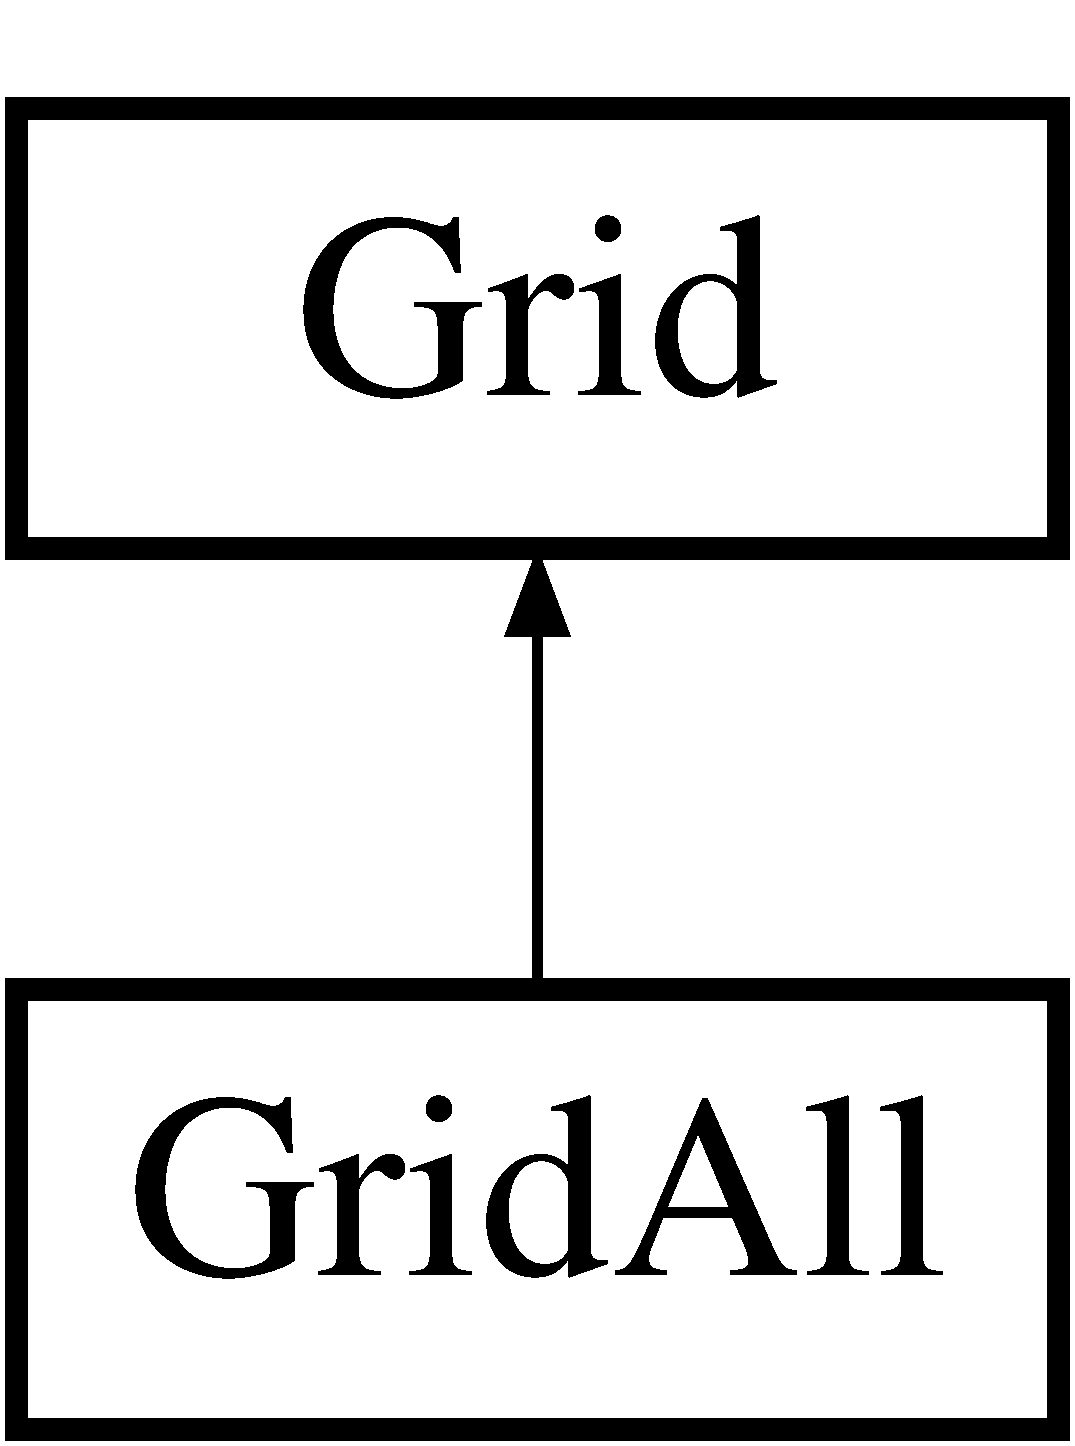
\includegraphics[height=2.000000cm]{class_grid_all}
\end{center}
\end{figure}
\subsection*{Metody publiczne}
\begin{DoxyCompactItemize}
\item 
\hyperlink{class_grid_all_a88d71f62359e7cd339f74a1a37e4b95f}{Grid\+All} ()
\begin{DoxyCompactList}\small\item\em Konstruktor. \end{DoxyCompactList}\item 
int \hyperlink{class_grid_all_aa513371e605fe9bea7489edfe3d40a1f}{Read\+Data} (map$<$ int, \hyperlink{class_point}{Point} $>$ \&Point\+Map, const string \&file, \hyperlink{class_simulation_parameters}{Simulation\+Parameters} \&sym\+\_\+param)
\end{DoxyCompactItemize}
\subsection*{Dodatkowe Dziedziczone Składowe}


\subsection{Opis szczegółowy}
Klasa Przygotowujaca siatke do symulacji. 

Zawiera funkcje potrzebne do przgotowania siatki, gdy z pliku wczytywane sa wspolrzedne pktow przeplywu, pole predkosci i tensor dyspersji dla wszytskich pkt przeplywu. 

Definicja w linii 239 pliku grid.\+h.



\subsection{Dokumentacja konstruktora i destruktora}
\hypertarget{class_grid_all_a88d71f62359e7cd339f74a1a37e4b95f}{}\index{Grid\+All@{Grid\+All}!Grid\+All@{Grid\+All}}
\index{Grid\+All@{Grid\+All}!Grid\+All@{Grid\+All}}
\subsubsection[{Grid\+All}]{\setlength{\rightskip}{0pt plus 5cm}Grid\+All\+::\+Grid\+All (
\begin{DoxyParamCaption}
{}
\end{DoxyParamCaption}
)\hspace{0.3cm}{\ttfamily [inline]}}\label{class_grid_all_a88d71f62359e7cd339f74a1a37e4b95f}


Konstruktor. 

Tworzy obiekt \hyperlink{class_grid}{Grid} All 

Definicja w linii 245 pliku grid.\+h.



\subsection{Dokumentacja funkcji składowych}
\hypertarget{class_grid_all_aa513371e605fe9bea7489edfe3d40a1f}{}\index{Grid\+All@{Grid\+All}!Read\+Data@{Read\+Data}}
\index{Read\+Data@{Read\+Data}!Grid\+All@{Grid\+All}}
\subsubsection[{Read\+Data}]{\setlength{\rightskip}{0pt plus 5cm}int Grid\+All\+::\+Read\+Data (
\begin{DoxyParamCaption}
\item[{map$<$ int, {\bf Point} $>$ \&}]{Point\+Map, }
\item[{const string \&}]{file, }
\item[{{\bf Simulation\+Parameters} \&}]{sym\+\_\+param}
\end{DoxyParamCaption}
)\hspace{0.3cm}{\ttfamily [virtual]}}\label{class_grid_all_aa513371e605fe9bea7489edfe3d40a1f}
Wczytywania dane z pliku wejsciowego do mapy punktow 
\begin{DoxyParams}{Parametry}
{\em Point\+Map} & -\/ referencja do Mapy Punktow \\
\hline
{\em file} & -\/ nazwa pliku z danymi \\
\hline
{\em sym\+\_\+param} & -\/ obiekt z parametrami symulacji \\
\hline
\end{DoxyParams}
obl max weartosci predkosci 

Reimplementowana z \hyperlink{class_grid_ac0cf78c28206fd44fba21c5a91d0a0e0}{Grid}.



Definicja w linii 660 pliku grid.\+cpp.



Dokumentacja dla tej klasy została wygenerowana z plików\+:\begin{DoxyCompactItemize}
\item 
\hyperlink{grid_8h}{grid.\+h}\item 
\hyperlink{grid_8cpp}{grid.\+cpp}\end{DoxyCompactItemize}

\hypertarget{class_grid_dispersion}{}\section{Dokumentacja klasy Grid\+Dispersion}
\label{class_grid_dispersion}\index{Grid\+Dispersion@{Grid\+Dispersion}}


Klasa Przygotowujaca siatke do symulacji.  




{\ttfamily \#include $<$grid.\+h$>$}

Diagram dziedziczenia dla Grid\+Dispersion\begin{figure}[H]
\begin{center}
\leavevmode
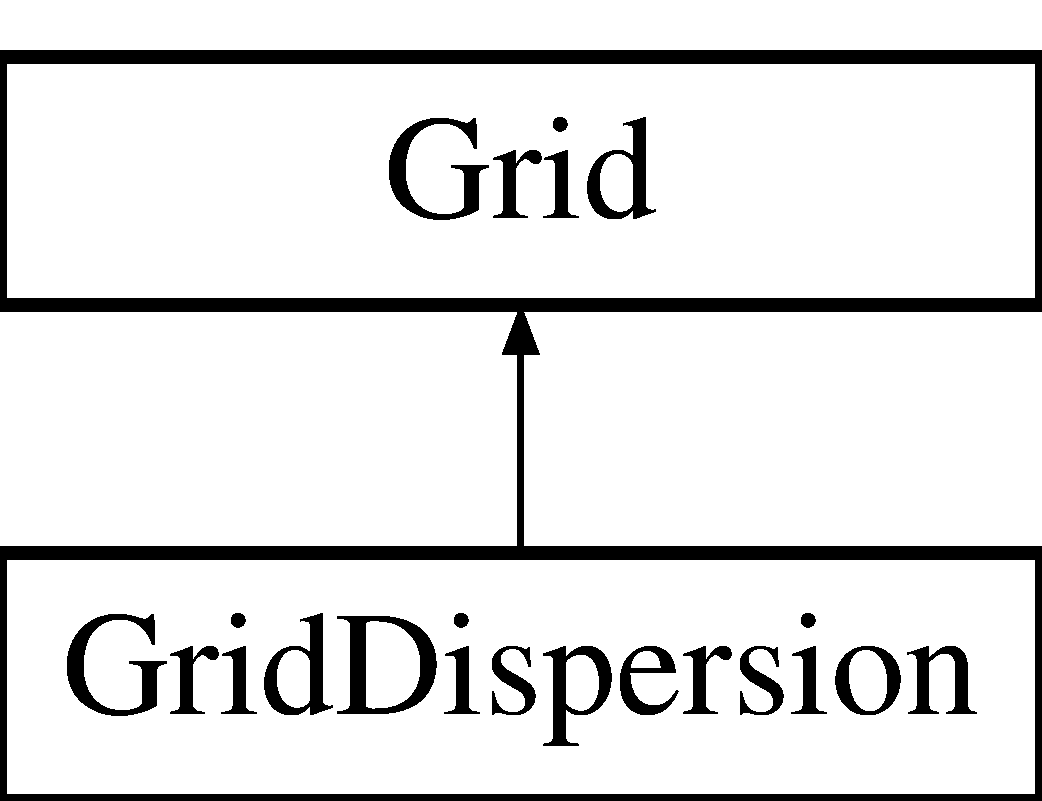
\includegraphics[height=2.000000cm]{class_grid_dispersion}
\end{center}
\end{figure}
\subsection*{Metody publiczne}
\begin{DoxyCompactItemize}
\item 
\hyperlink{class_grid_dispersion_aa91ae00919a4f12049f9415e3b584b31}{Grid\+Dispersion} ()
\begin{DoxyCompactList}\small\item\em Konstruktor. \end{DoxyCompactList}\item 
int \hyperlink{class_grid_dispersion_afbc03fca9459c90c19959c24df944766}{Read\+Data} (map$<$ int, \hyperlink{class_point}{Point} $>$ \&Point\+Map, const string \&file, \hyperlink{class_simulation_parameters}{Simulation\+Parameters} \&sym\+\_\+param)
\end{DoxyCompactItemize}
\subsection*{Dodatkowe Dziedziczone Składowe}


\subsection{Opis szczegółowy}
Klasa Przygotowujaca siatke do symulacji. 

Zawiera funkcje potrzebne do przgotowania siatki, gdy z pliku wczytywane sa wspolrzedne pktow przeplywu i wartosci wspolczynnikow dyspersji, a skladowe predkosci sa stale na calej siatce. 

Definicja w linii 258 pliku grid.\+h.



\subsection{Dokumentacja konstruktora i destruktora}
\hypertarget{class_grid_dispersion_aa91ae00919a4f12049f9415e3b584b31}{}\index{Grid\+Dispersion@{Grid\+Dispersion}!Grid\+Dispersion@{Grid\+Dispersion}}
\index{Grid\+Dispersion@{Grid\+Dispersion}!Grid\+Dispersion@{Grid\+Dispersion}}
\subsubsection[{Grid\+Dispersion}]{\setlength{\rightskip}{0pt plus 5cm}Grid\+Dispersion\+::\+Grid\+Dispersion (
\begin{DoxyParamCaption}
{}
\end{DoxyParamCaption}
)\hspace{0.3cm}{\ttfamily [inline]}}\label{class_grid_dispersion_aa91ae00919a4f12049f9415e3b584b31}


Konstruktor. 

Tworzy obiekt \hyperlink{class_grid}{Grid} Dispersion 

Definicja w linii 264 pliku grid.\+h.



\subsection{Dokumentacja funkcji składowych}
\hypertarget{class_grid_dispersion_afbc03fca9459c90c19959c24df944766}{}\index{Grid\+Dispersion@{Grid\+Dispersion}!Read\+Data@{Read\+Data}}
\index{Read\+Data@{Read\+Data}!Grid\+Dispersion@{Grid\+Dispersion}}
\subsubsection[{Read\+Data}]{\setlength{\rightskip}{0pt plus 5cm}int Grid\+Dispersion\+::\+Read\+Data (
\begin{DoxyParamCaption}
\item[{map$<$ int, {\bf Point} $>$ \&}]{Point\+Map, }
\item[{const string \&}]{file, }
\item[{{\bf Simulation\+Parameters} \&}]{sym\+\_\+param}
\end{DoxyParamCaption}
)\hspace{0.3cm}{\ttfamily [virtual]}}\label{class_grid_dispersion_afbc03fca9459c90c19959c24df944766}
Wczytywania dane z pliku wejsciowego do mapy punktow 
\begin{DoxyParams}{Parametry}
{\em Point\+Map} & -\/ referencja do Mapy Punktow \\
\hline
{\em file} & -\/ nazwa pliku z danymi \\
\hline
{\em sym\+\_\+param} & -\/ obiekt z parametrami symulacji \\
\hline
\end{DoxyParams}


Reimplementowana z \hyperlink{class_grid_ac0cf78c28206fd44fba21c5a91d0a0e0}{Grid}.



Definicja w linii 726 pliku grid.\+cpp.



Dokumentacja dla tej klasy została wygenerowana z plików\+:\begin{DoxyCompactItemize}
\item 
\hyperlink{grid_8h}{grid.\+h}\item 
\hyperlink{grid_8cpp}{grid.\+cpp}\end{DoxyCompactItemize}

\hypertarget{class_grid_only}{}\section{Dokumentacja klasy Grid\+Only}
\label{class_grid_only}\index{Grid\+Only@{Grid\+Only}}


Klasa Przygotowujaca siatke do symulacji.  




{\ttfamily \#include $<$grid.\+h$>$}

Diagram dziedziczenia dla Grid\+Only\begin{figure}[H]
\begin{center}
\leavevmode
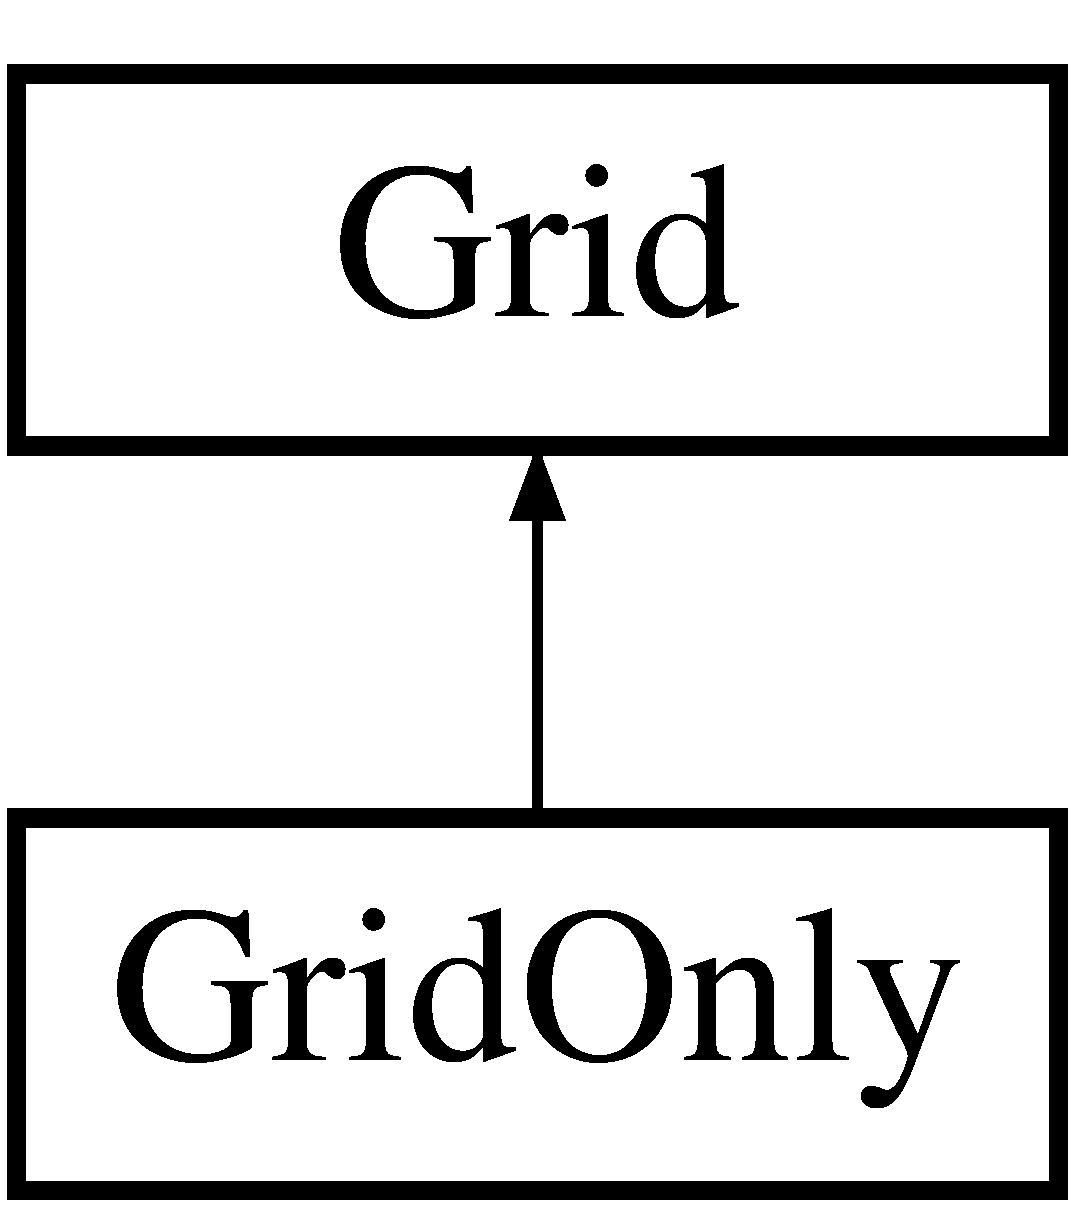
\includegraphics[height=2.000000cm]{class_grid_only}
\end{center}
\end{figure}
\subsection*{Metody publiczne}
\begin{DoxyCompactItemize}
\item 
\hyperlink{class_grid_only_a71437d24648d7d4db8836eefbda7a360}{Grid\+Only} ()
\begin{DoxyCompactList}\small\item\em Konstruktor. \end{DoxyCompactList}\item 
int \hyperlink{class_grid_only_a86e143a957ba61c0a5b215b65ea24902}{Read\+Data} (map$<$ int, \hyperlink{class_point}{Point} $>$ \&Point\+Map, const string \&file, \hyperlink{class_simulation_parameters}{Simulation\+Parameters} \&sym\+\_\+param)
\end{DoxyCompactItemize}
\subsection*{Dodatkowe Dziedziczone Składowe}


\subsection{Opis szczegółowy}
Klasa Przygotowujaca siatke do symulacji. 

Zawiera funkcje potrzebne do przgotowania siatki, gdy z pliku wczytywane sa tylko wspolrzedne pktow przeplywu, a wartosci predkosci i wspolczynniki dyspersji sa stale na calej siatce. 

Definicja w linii 197 pliku grid.\+h.



\subsection{Dokumentacja konstruktora i destruktora}
\hypertarget{class_grid_only_a71437d24648d7d4db8836eefbda7a360}{}\index{Grid\+Only@{Grid\+Only}!Grid\+Only@{Grid\+Only}}
\index{Grid\+Only@{Grid\+Only}!Grid\+Only@{Grid\+Only}}
\subsubsection[{Grid\+Only}]{\setlength{\rightskip}{0pt plus 5cm}Grid\+Only\+::\+Grid\+Only (
\begin{DoxyParamCaption}
{}
\end{DoxyParamCaption}
)\hspace{0.3cm}{\ttfamily [inline]}}\label{class_grid_only_a71437d24648d7d4db8836eefbda7a360}


Konstruktor. 

Tworzy obiekt \hyperlink{class_grid}{Grid} Only 

Definicja w linii 204 pliku grid.\+h.



\subsection{Dokumentacja funkcji składowych}
\hypertarget{class_grid_only_a86e143a957ba61c0a5b215b65ea24902}{}\index{Grid\+Only@{Grid\+Only}!Read\+Data@{Read\+Data}}
\index{Read\+Data@{Read\+Data}!Grid\+Only@{Grid\+Only}}
\subsubsection[{Read\+Data}]{\setlength{\rightskip}{0pt plus 5cm}int Grid\+Only\+::\+Read\+Data (
\begin{DoxyParamCaption}
\item[{map$<$ int, {\bf Point} $>$ \&}]{Point\+Map, }
\item[{const string \&}]{file, }
\item[{{\bf Simulation\+Parameters} \&}]{sym\+\_\+param}
\end{DoxyParamCaption}
)\hspace{0.3cm}{\ttfamily [virtual]}}\label{class_grid_only_a86e143a957ba61c0a5b215b65ea24902}
Wczytywania dane z pliku wejsciowego do mapy punktow 
\begin{DoxyParams}{Parametry}
{\em Point\+Map} & -\/ referencja do Mapy Punktow \\
\hline
{\em file} & -\/ nazwa pliku z danymi \\
\hline
{\em sym\+\_\+param} & -\/ obiekt z parametrami symulacji \\
\hline
\end{DoxyParams}


Reimplementowana z \hyperlink{class_grid_ac0cf78c28206fd44fba21c5a91d0a0e0}{Grid}.



Definicja w linii 520 pliku grid.\+cpp.



Dokumentacja dla tej klasy została wygenerowana z plików\+:\begin{DoxyCompactItemize}
\item 
\hyperlink{grid_8h}{grid.\+h}\item 
\hyperlink{grid_8cpp}{grid.\+cpp}\end{DoxyCompactItemize}

\hypertarget{class_grid_velocity}{}\section{Dokumentacja klasy Grid\+Velocity}
\label{class_grid_velocity}\index{Grid\+Velocity@{Grid\+Velocity}}


Klasa Przygotowujaca siatke do symulacji.  




{\ttfamily \#include $<$grid.\+h$>$}

Diagram dziedziczenia dla Grid\+Velocity\begin{figure}[H]
\begin{center}
\leavevmode
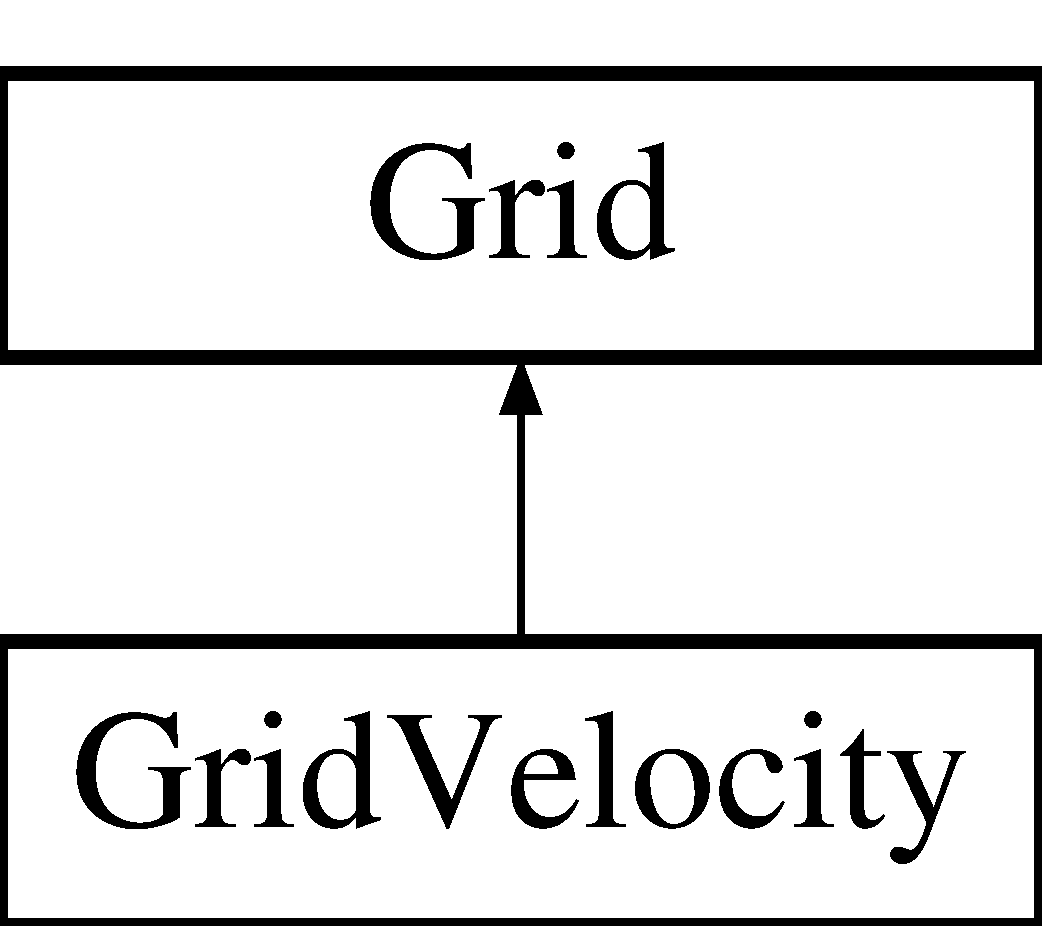
\includegraphics[height=2.000000cm]{class_grid_velocity}
\end{center}
\end{figure}
\subsection*{Metody publiczne}
\begin{DoxyCompactItemize}
\item 
\hyperlink{class_grid_velocity_afdff39055c5fcd27eb8473cca1fee826}{Grid\+Velocity} ()
\begin{DoxyCompactList}\small\item\em Konstruktor. \end{DoxyCompactList}\item 
int \hyperlink{class_grid_velocity_a00143f2982252ae30ceb725886c11ab6}{Read\+Data} (map$<$ int, \hyperlink{class_point}{Point} $>$ \&Point\+Map, const string \&file, \hyperlink{class_simulation_parameters}{Simulation\+Parameters} \&sym\+\_\+param)
\end{DoxyCompactItemize}
\subsection*{Dodatkowe Dziedziczone Składowe}


\subsection{Opis szczegółowy}
Klasa Przygotowujaca siatke do symulacji. 

Zawiera funkcje potrzebne do przgotowania siatki, gdy z pliku wczytywane sa wspolrzedne pktow przeplywu i pole predkosci a wartosci wspolczynnikow dyspersji sa stale na calej siatce. 

Definicja w linii 220 pliku grid.\+h.



\subsection{Dokumentacja konstruktora i destruktora}
\hypertarget{class_grid_velocity_afdff39055c5fcd27eb8473cca1fee826}{}\index{Grid\+Velocity@{Grid\+Velocity}!Grid\+Velocity@{Grid\+Velocity}}
\index{Grid\+Velocity@{Grid\+Velocity}!Grid\+Velocity@{Grid\+Velocity}}
\subsubsection[{Grid\+Velocity}]{\setlength{\rightskip}{0pt plus 5cm}Grid\+Velocity\+::\+Grid\+Velocity (
\begin{DoxyParamCaption}
{}
\end{DoxyParamCaption}
)\hspace{0.3cm}{\ttfamily [inline]}}\label{class_grid_velocity_afdff39055c5fcd27eb8473cca1fee826}


Konstruktor. 

Tworzy obiekt \hyperlink{class_grid}{Grid} Velocity 

Definicja w linii 226 pliku grid.\+h.



\subsection{Dokumentacja funkcji składowych}
\hypertarget{class_grid_velocity_a00143f2982252ae30ceb725886c11ab6}{}\index{Grid\+Velocity@{Grid\+Velocity}!Read\+Data@{Read\+Data}}
\index{Read\+Data@{Read\+Data}!Grid\+Velocity@{Grid\+Velocity}}
\subsubsection[{Read\+Data}]{\setlength{\rightskip}{0pt plus 5cm}int Grid\+Velocity\+::\+Read\+Data (
\begin{DoxyParamCaption}
\item[{map$<$ int, {\bf Point} $>$ \&}]{Point\+Map, }
\item[{const string \&}]{file, }
\item[{{\bf Simulation\+Parameters} \&}]{sym\+\_\+param}
\end{DoxyParamCaption}
)\hspace{0.3cm}{\ttfamily [virtual]}}\label{class_grid_velocity_a00143f2982252ae30ceb725886c11ab6}
Wczytywania dane z pliku wejsciowego do mapy punktow 
\begin{DoxyParams}{Parametry}
{\em Point\+Map} & -\/ referencja do Mapy Punktow \\
\hline
{\em file} & -\/ nazwa pliku z danymi \\
\hline
{\em sym\+\_\+param} & -\/ obiekt z parametrami symulacji \\
\hline
\end{DoxyParams}
obl max weartosci predkosci 

Reimplementowana z \hyperlink{class_grid_ac0cf78c28206fd44fba21c5a91d0a0e0}{Grid}.



Definicja w linii 591 pliku grid.\+cpp.



Dokumentacja dla tej klasy została wygenerowana z plików\+:\begin{DoxyCompactItemize}
\item 
\hyperlink{grid_8h}{grid.\+h}\item 
\hyperlink{grid_8cpp}{grid.\+cpp}\end{DoxyCompactItemize}

\hypertarget{class_net_heat_flux}{}\section{Dokumentacja klasy Net\+Heat\+Flux}
\label{class_net_heat_flux}\index{Net\+Heat\+Flux@{Net\+Heat\+Flux}}


Klasa do obliczen członu źródłowego wyminay ciepla z atmosfera.  




{\ttfamily \#include $<$netheatflux.\+h$>$}

\subsection*{Metody publiczne}
\begin{DoxyCompactItemize}
\item 
\hyperlink{class_net_heat_flux_a6e4c7b7a65cc582fe7f812b10d8dd0ae}{Net\+Heat\+Flux} ()
\begin{DoxyCompactList}\small\item\em Konstruktor. \end{DoxyCompactList}\item 
\hyperlink{class_net_heat_flux_a49a9703237a48c6851464376b0892246}{Net\+Heat\+Flux} (double Ta, double Rh, double pa, double Js, double u)
\item 
long double \hyperlink{class_net_heat_flux_a31570d0c05e45b2a01a05b3976617ac4}{Compute\+Net\+Heat\+Flux} (long double Tw)
\begin{DoxyCompactList}\small\item\em oblicza wartosc czlonu zródłowego \end{DoxyCompactList}\item 
long double \hyperlink{class_net_heat_flux_a5bf457660c754e02562840cc90cf00ac}{Compute\+Net\+Solar} ()
\begin{DoxyCompactList}\small\item\em oblicza wartosc promieniowania słonecznego krotkofalowe \end{DoxyCompactList}\item 
long double \hyperlink{class_net_heat_flux_a8c35767d0fdf37fd6216e0c2f1e71cc2}{Compute\+Long\+Wave\+Atmosf} ()
\begin{DoxyCompactList}\small\item\em oblicza wartosc promieniowania atmosferycznego długofalowego \end{DoxyCompactList}\item 
long double \hyperlink{class_net_heat_flux_a87b1a80ed14554fcaf903a3383f25a77}{Emissivity\+\_\+\+Brunt1932} (double a1=0.\+55, double a2=0.\+065)
\begin{DoxyCompactList}\small\item\em oblicza wartosc emisyjnosci atmosfery wg formuły podanej przez Brunt (1932) \end{DoxyCompactList}\item 
long double \hyperlink{class_net_heat_flux_a867bd311aaaf67ba057ad24f8e8ba5af}{Compute\+Long\+Wave\+Water} (long double \&Tw)
\begin{DoxyCompactList}\small\item\em oblicza wartosc promieniowania długofalowego W\+O\+D\+Y \end{DoxyCompactList}\item 
long double \hyperlink{class_net_heat_flux_a7029244ff808627ebc74a9e74d00abe4}{Compute\+Evap\+Condens} (long double \&Tw)
\begin{DoxyCompactList}\small\item\em oblicza wartosc strat ciepła zwiazanego z praowaniem \end{DoxyCompactList}\item 
long double \hyperlink{class_net_heat_flux_a3209796cc63c1b6f1d8040f7bb815053}{Wind\+Function\+\_\+\+Chapra2008} (float c1=19.\+0, float c2=0.\+95)
\begin{DoxyCompactList}\small\item\em oblicza wartosc funkcji zależnej od predkosci waitru oblicza wartosc funkcji zależnej od predkosci waitru wg zależnosci f(u) = c1 + c2 u$^\wedge$2 -\/ domyślnie c1 = 19.\+0, c2 = 0.\+95 -\/ Chapra 2008, Edinger et al 1974 \end{DoxyCompactList}\item 
long double \hyperlink{class_net_heat_flux_ab3807fc076b38645302be22d62c70c65}{Compute\+Cond\+Conv} (long double \&Tw)
\begin{DoxyCompactList}\small\item\em oblicza wartosc strumienia ciepła w wyniku przewodzenia i konwekscji \end{DoxyCompactList}\item 
double \hyperlink{class_net_heat_flux_a495d266066abc2afdfc6f67e73e9f5d6}{get\+\_\+\+Ta} () const 
\item 
double \hyperlink{class_net_heat_flux_aaf841691bf132c9b7d26c7ff3a60b798}{get\+\_\+\+Rh} () const 
\item 
double \hyperlink{class_net_heat_flux_ab6d1ce8e3f2f4034c256bd32b9285b01}{get\+\_\+pa} () const 
\item 
double \hyperlink{class_net_heat_flux_a37bddd6b4413bf9a4265b0e6121dc53a}{get\+\_\+\+Js} () const 
\item 
double \hyperlink{class_net_heat_flux_ad5d42768c59f90e629dd033a6fd1ac77}{get\+\_\+u} () const 
\item 
double \hyperlink{class_net_heat_flux_a1f7f06ac4ad2d3e71a2c9c7203ffc833}{get\+\_\+aw} () const 
\item 
double \hyperlink{class_net_heat_flux_a1a1c94edb55d10722782ac1e76f1c8b8}{get\+\_\+ea} () const 
\item 
double \hyperlink{class_net_heat_flux_ab48ea591c24a62581348cc291d565076}{get\+\_\+emis\+\_\+w} () const 
\item 
void \hyperlink{class_net_heat_flux_a9e9700acebfa6481f24b93c2f7d1efd6}{set\+\_\+\+Ta} (double Ta)
\item 
void \hyperlink{class_net_heat_flux_a870e6db2db832d88f88a0f75516f39d7}{set\+\_\+\+Rh} (double Rh)
\item 
void \hyperlink{class_net_heat_flux_ac4d58893c28e07cd05a7988d098df46b}{set\+\_\+pa} (double pa)
\item 
void \hyperlink{class_net_heat_flux_a4608ba4ec5bade409d066b9e2370a4a0}{set\+\_\+\+Js} (double Js)
\item 
void \hyperlink{class_net_heat_flux_ac4c880ee001af382d098191843b4fafb}{set\+\_\+u} (double u)
\item 
void \hyperlink{class_net_heat_flux_a4f17f1801cbea3b76715fdc873be78b6}{set\+\_\+aw} (double aw=0.\+06)
\item 
void \hyperlink{class_net_heat_flux_ae90ff0b43ec0e41e2f40f28df7c9612d}{set\+\_\+ea} ()
\item 
long double \hyperlink{class_net_heat_flux_a3baa4ec5f1504d7e5c01efd21530637f}{e\+\_\+sat} (long double T, double b1=6.\+12, double b2=17.\+27, double b3=237.\+3)
\item 
void \hyperlink{class_net_heat_flux_ac6c12bccd613d87ffae5a90b4910eaeb}{set\+\_\+emis\+\_\+w} (double emis\+\_\+w=0.\+97)
\item 
void \hyperlink{class_net_heat_flux_ae127a9c31f1bd777f40b9034395d4f96}{set\+\_\+cb} (double cb=0.\+62)
\end{DoxyCompactItemize}


\subsection{Opis szczegółowy}
Klasa do obliczen członu źródłowego wyminay ciepla z atmosfera. 

Zawiera metody potrzebane do wyznaczenia wratosci wypadkowego strumienia ciepła na granicy woda powietrze 

Definicja w linii 23 pliku netheatflux.\+h.



\subsection{Dokumentacja konstruktora i destruktora}
\hypertarget{class_net_heat_flux_a6e4c7b7a65cc582fe7f812b10d8dd0ae}{}\index{Net\+Heat\+Flux@{Net\+Heat\+Flux}!Net\+Heat\+Flux@{Net\+Heat\+Flux}}
\index{Net\+Heat\+Flux@{Net\+Heat\+Flux}!Net\+Heat\+Flux@{Net\+Heat\+Flux}}
\subsubsection[{Net\+Heat\+Flux}]{\setlength{\rightskip}{0pt plus 5cm}Net\+Heat\+Flux\+::\+Net\+Heat\+Flux (
\begin{DoxyParamCaption}
{}
\end{DoxyParamCaption}
)\hspace{0.3cm}{\ttfamily [inline]}}\label{class_net_heat_flux_a6e4c7b7a65cc582fe7f812b10d8dd0ae}


Konstruktor. 

Tworzy obiekt \hyperlink{class_net_heat_flux}{Net\+Heat\+Flux} 

Definicja w linii 31 pliku netheatflux.\+h.

\hypertarget{class_net_heat_flux_a49a9703237a48c6851464376b0892246}{}\index{Net\+Heat\+Flux@{Net\+Heat\+Flux}!Net\+Heat\+Flux@{Net\+Heat\+Flux}}
\index{Net\+Heat\+Flux@{Net\+Heat\+Flux}!Net\+Heat\+Flux@{Net\+Heat\+Flux}}
\subsubsection[{Net\+Heat\+Flux}]{\setlength{\rightskip}{0pt plus 5cm}Net\+Heat\+Flux\+::\+Net\+Heat\+Flux (
\begin{DoxyParamCaption}
\item[{double}]{Ta, }
\item[{double}]{Rh, }
\item[{double}]{pa, }
\item[{double}]{Js, }
\item[{double}]{u}
\end{DoxyParamCaption}
)\hspace{0.3cm}{\ttfamily [inline]}}\label{class_net_heat_flux_a49a9703237a48c6851464376b0892246}


Definicja w linii 35 pliku netheatflux.\+h.



\subsection{Dokumentacja funkcji składowych}
\hypertarget{class_net_heat_flux_ab3807fc076b38645302be22d62c70c65}{}\index{Net\+Heat\+Flux@{Net\+Heat\+Flux}!Compute\+Cond\+Conv@{Compute\+Cond\+Conv}}
\index{Compute\+Cond\+Conv@{Compute\+Cond\+Conv}!Net\+Heat\+Flux@{Net\+Heat\+Flux}}
\subsubsection[{Compute\+Cond\+Conv}]{\setlength{\rightskip}{0pt plus 5cm}long double Net\+Heat\+Flux\+::\+Compute\+Cond\+Conv (
\begin{DoxyParamCaption}
\item[{long double \&}]{Tw}
\end{DoxyParamCaption}
)}\label{class_net_heat_flux_ab3807fc076b38645302be22d62c70c65}


oblicza wartosc strumienia ciepła w wyniku przewodzenia i konwekscji 

Oblicza wartosc strumienia ciepła w wyniku przewodzenia i konwekscji 
\begin{DoxyParams}{Parametry}
{\em Tw} & -\/ temp wody \\
\hline
\end{DoxyParams}
\begin{DoxyReturn}{Zwraca}
wartosc strumienia ciepła w wyniku przewodzenia i konwekscji 
\end{DoxyReturn}


Definicja w linii 106 pliku netheatflux.\+cpp.

\hypertarget{class_net_heat_flux_a7029244ff808627ebc74a9e74d00abe4}{}\index{Net\+Heat\+Flux@{Net\+Heat\+Flux}!Compute\+Evap\+Condens@{Compute\+Evap\+Condens}}
\index{Compute\+Evap\+Condens@{Compute\+Evap\+Condens}!Net\+Heat\+Flux@{Net\+Heat\+Flux}}
\subsubsection[{Compute\+Evap\+Condens}]{\setlength{\rightskip}{0pt plus 5cm}long double Net\+Heat\+Flux\+::\+Compute\+Evap\+Condens (
\begin{DoxyParamCaption}
\item[{long double \&}]{Tw}
\end{DoxyParamCaption}
)}\label{class_net_heat_flux_a7029244ff808627ebc74a9e74d00abe4}


oblicza wartosc strat ciepła zwiazanego z praowaniem 

Oblicza wartosc strat ciepła zwiazanego z parowaniem lub dostarcenia ciepła związnego z procesem kondensacji 
\begin{DoxyParams}{Parametry}
{\em Tw} & -\/ temp wody \\
\hline
\end{DoxyParams}
\begin{DoxyReturn}{Zwraca}
wartosc strumienia energii w wyniku parowania/kondenscji pary wodnej 
\end{DoxyReturn}


Definicja w linii 91 pliku netheatflux.\+cpp.

\hypertarget{class_net_heat_flux_a8c35767d0fdf37fd6216e0c2f1e71cc2}{}\index{Net\+Heat\+Flux@{Net\+Heat\+Flux}!Compute\+Long\+Wave\+Atmosf@{Compute\+Long\+Wave\+Atmosf}}
\index{Compute\+Long\+Wave\+Atmosf@{Compute\+Long\+Wave\+Atmosf}!Net\+Heat\+Flux@{Net\+Heat\+Flux}}
\subsubsection[{Compute\+Long\+Wave\+Atmosf}]{\setlength{\rightskip}{0pt plus 5cm}long double Net\+Heat\+Flux\+::\+Compute\+Long\+Wave\+Atmosf (
\begin{DoxyParamCaption}
{}
\end{DoxyParamCaption}
)}\label{class_net_heat_flux_a8c35767d0fdf37fd6216e0c2f1e71cc2}


oblicza wartosc promieniowania atmosferycznego długofalowego 


\begin{DoxyParams}{Parametry}
{\em -\/} & \\
\hline
\end{DoxyParams}
\begin{DoxyReturn}{Zwraca}
wartosc promieniowania atmosferycznego długofalowego 
\end{DoxyReturn}


Definicja w linii 40 pliku netheatflux.\+cpp.

\hypertarget{class_net_heat_flux_a867bd311aaaf67ba057ad24f8e8ba5af}{}\index{Net\+Heat\+Flux@{Net\+Heat\+Flux}!Compute\+Long\+Wave\+Water@{Compute\+Long\+Wave\+Water}}
\index{Compute\+Long\+Wave\+Water@{Compute\+Long\+Wave\+Water}!Net\+Heat\+Flux@{Net\+Heat\+Flux}}
\subsubsection[{Compute\+Long\+Wave\+Water}]{\setlength{\rightskip}{0pt plus 5cm}long double Net\+Heat\+Flux\+::\+Compute\+Long\+Wave\+Water (
\begin{DoxyParamCaption}
\item[{long double \&}]{Tw}
\end{DoxyParamCaption}
)}\label{class_net_heat_flux_a867bd311aaaf67ba057ad24f8e8ba5af}


oblicza wartosc promieniowania długofalowego W\+O\+D\+Y 

Oblicza wartosc promieniowania długofalowego W\+O\+D\+Y kożystając z prawa Stefana-\/\+Boltzmana 
\begin{DoxyParams}{Parametry}
{\em Tw} & -\/ temp wody \\
\hline
\end{DoxyParams}
\begin{DoxyReturn}{Zwraca}
wartosc promieniowania długofalowego wody 
\end{DoxyReturn}


Definicja w linii 83 pliku netheatflux.\+cpp.

\hypertarget{class_net_heat_flux_a31570d0c05e45b2a01a05b3976617ac4}{}\index{Net\+Heat\+Flux@{Net\+Heat\+Flux}!Compute\+Net\+Heat\+Flux@{Compute\+Net\+Heat\+Flux}}
\index{Compute\+Net\+Heat\+Flux@{Compute\+Net\+Heat\+Flux}!Net\+Heat\+Flux@{Net\+Heat\+Flux}}
\subsubsection[{Compute\+Net\+Heat\+Flux}]{\setlength{\rightskip}{0pt plus 5cm}long double Net\+Heat\+Flux\+::\+Compute\+Net\+Heat\+Flux (
\begin{DoxyParamCaption}
\item[{long double}]{Tw}
\end{DoxyParamCaption}
)}\label{class_net_heat_flux_a31570d0c05e45b2a01a05b3976617ac4}


oblicza wartosc czlonu zródłowego 

Oblicza wartosc czlonu zrodlowego dla danej temp wody na podstawie podsnaych danych meteorologicznych


\begin{DoxyParams}{Parametry}
{\em Tw} & -\/ wartość temperatury wody dla ktorej ma być obliczony czlon zrodlowy \\
\hline
\end{DoxyParams}
\begin{DoxyReturn}{Zwraca}
wartosc czlonu zrodlowego dla danej temp 
\end{DoxyReturn}


Definicja w linii 16 pliku netheatflux.\+cpp.

\hypertarget{class_net_heat_flux_a5bf457660c754e02562840cc90cf00ac}{}\index{Net\+Heat\+Flux@{Net\+Heat\+Flux}!Compute\+Net\+Solar@{Compute\+Net\+Solar}}
\index{Compute\+Net\+Solar@{Compute\+Net\+Solar}!Net\+Heat\+Flux@{Net\+Heat\+Flux}}
\subsubsection[{Compute\+Net\+Solar}]{\setlength{\rightskip}{0pt plus 5cm}long double Net\+Heat\+Flux\+::\+Compute\+Net\+Solar (
\begin{DoxyParamCaption}
{}
\end{DoxyParamCaption}
)}\label{class_net_heat_flux_a5bf457660c754e02562840cc90cf00ac}


oblicza wartosc promieniowania słonecznego krotkofalowe 

Oblicza wartosc promieniowania słonecznego krotkofalowego na podstawie pomiarów promieniowania słonecznego padającego oraz albedo wody

\begin{DoxyReturn}{Zwraca}
wartosc promieniowania słonecznego krotkofalowe 
\end{DoxyReturn}


Definicja w linii 32 pliku netheatflux.\+cpp.

\hypertarget{class_net_heat_flux_a3baa4ec5f1504d7e5c01efd21530637f}{}\index{Net\+Heat\+Flux@{Net\+Heat\+Flux}!e\+\_\+sat@{e\+\_\+sat}}
\index{e\+\_\+sat@{e\+\_\+sat}!Net\+Heat\+Flux@{Net\+Heat\+Flux}}
\subsubsection[{e\+\_\+sat}]{\setlength{\rightskip}{0pt plus 5cm}long double Net\+Heat\+Flux\+::e\+\_\+sat (
\begin{DoxyParamCaption}
\item[{long double}]{T, }
\item[{double}]{b1 = {\ttfamily 6.12}, }
\item[{double}]{b2 = {\ttfamily 17.27}, }
\item[{double}]{b3 = {\ttfamily 237.3}}
\end{DoxyParamCaption}
)}\label{class_net_heat_flux_a3baa4ec5f1504d7e5c01efd21530637f}
oblicza wartosc prężności (ciśnienia) pary wodnej (defoltowo wg formuly Raudkivi 1979, Chapra 1997\+: 6.\+12 exp(17.\+27$\ast$\+Ta/(Ta+237.3)) 

Definicja w linii 77 pliku netheatflux.\+cpp.

\hypertarget{class_net_heat_flux_a87b1a80ed14554fcaf903a3383f25a77}{}\index{Net\+Heat\+Flux@{Net\+Heat\+Flux}!Emissivity\+\_\+\+Brunt1932@{Emissivity\+\_\+\+Brunt1932}}
\index{Emissivity\+\_\+\+Brunt1932@{Emissivity\+\_\+\+Brunt1932}!Net\+Heat\+Flux@{Net\+Heat\+Flux}}
\subsubsection[{Emissivity\+\_\+\+Brunt1932}]{\setlength{\rightskip}{0pt plus 5cm}long double Net\+Heat\+Flux\+::\+Emissivity\+\_\+\+Brunt1932 (
\begin{DoxyParamCaption}
\item[{double}]{a1 = {\ttfamily 0.55}, }
\item[{double}]{a2 = {\ttfamily 0.065}}
\end{DoxyParamCaption}
)}\label{class_net_heat_flux_a87b1a80ed14554fcaf903a3383f25a77}


oblicza wartosc emisyjnosci atmosfery wg formuły podanej przez Brunt (1932) 


\begin{DoxyParams}{Parametry}
{\em a1} & -\/ coefficient \mbox{[}\mbox{]} \\
\hline
{\em a2} & -\/ coefficient \mbox{[}h\+Pa$^\wedge$(-\/1/2)\mbox{]} \\
\hline
\end{DoxyParams}
\begin{DoxyReturn}{Zwraca}
wartosc emisyjnosci atmosfery 
\end{DoxyReturn}


Definicja w linii 49 pliku netheatflux.\+cpp.

\hypertarget{class_net_heat_flux_a1f7f06ac4ad2d3e71a2c9c7203ffc833}{}\index{Net\+Heat\+Flux@{Net\+Heat\+Flux}!get\+\_\+aw@{get\+\_\+aw}}
\index{get\+\_\+aw@{get\+\_\+aw}!Net\+Heat\+Flux@{Net\+Heat\+Flux}}
\subsubsection[{get\+\_\+aw}]{\setlength{\rightskip}{0pt plus 5cm}double Net\+Heat\+Flux\+::get\+\_\+aw (
\begin{DoxyParamCaption}
{}
\end{DoxyParamCaption}
) const\hspace{0.3cm}{\ttfamily [inline]}}\label{class_net_heat_flux_a1f7f06ac4ad2d3e71a2c9c7203ffc833}
zwraca wartosc albedo wody 

Definicja w linii 154 pliku netheatflux.\+h.

\hypertarget{class_net_heat_flux_a1a1c94edb55d10722782ac1e76f1c8b8}{}\index{Net\+Heat\+Flux@{Net\+Heat\+Flux}!get\+\_\+ea@{get\+\_\+ea}}
\index{get\+\_\+ea@{get\+\_\+ea}!Net\+Heat\+Flux@{Net\+Heat\+Flux}}
\subsubsection[{get\+\_\+ea}]{\setlength{\rightskip}{0pt plus 5cm}double Net\+Heat\+Flux\+::get\+\_\+ea (
\begin{DoxyParamCaption}
{}
\end{DoxyParamCaption}
) const\hspace{0.3cm}{\ttfamily [inline]}}\label{class_net_heat_flux_a1a1c94edb55d10722782ac1e76f1c8b8}
zwraca wartosc aktualnej prężności (ciśnienia) pary wodnej w powietrzu 

Definicja w linii 159 pliku netheatflux.\+h.

\hypertarget{class_net_heat_flux_ab48ea591c24a62581348cc291d565076}{}\index{Net\+Heat\+Flux@{Net\+Heat\+Flux}!get\+\_\+emis\+\_\+w@{get\+\_\+emis\+\_\+w}}
\index{get\+\_\+emis\+\_\+w@{get\+\_\+emis\+\_\+w}!Net\+Heat\+Flux@{Net\+Heat\+Flux}}
\subsubsection[{get\+\_\+emis\+\_\+w}]{\setlength{\rightskip}{0pt plus 5cm}double Net\+Heat\+Flux\+::get\+\_\+emis\+\_\+w (
\begin{DoxyParamCaption}
{}
\end{DoxyParamCaption}
) const\hspace{0.3cm}{\ttfamily [inline]}}\label{class_net_heat_flux_ab48ea591c24a62581348cc291d565076}
zwraca wartosc ustawionej zdolności emisyjnej wody 

Definicja w linii 164 pliku netheatflux.\+h.

\hypertarget{class_net_heat_flux_a37bddd6b4413bf9a4265b0e6121dc53a}{}\index{Net\+Heat\+Flux@{Net\+Heat\+Flux}!get\+\_\+\+Js@{get\+\_\+\+Js}}
\index{get\+\_\+\+Js@{get\+\_\+\+Js}!Net\+Heat\+Flux@{Net\+Heat\+Flux}}
\subsubsection[{get\+\_\+\+Js}]{\setlength{\rightskip}{0pt plus 5cm}double Net\+Heat\+Flux\+::get\+\_\+\+Js (
\begin{DoxyParamCaption}
{}
\end{DoxyParamCaption}
) const\hspace{0.3cm}{\ttfamily [inline]}}\label{class_net_heat_flux_a37bddd6b4413bf9a4265b0e6121dc53a}
zwraca wartosc promieniowania krotkofalowego 

Definicja w linii 144 pliku netheatflux.\+h.

\hypertarget{class_net_heat_flux_ab6d1ce8e3f2f4034c256bd32b9285b01}{}\index{Net\+Heat\+Flux@{Net\+Heat\+Flux}!get\+\_\+pa@{get\+\_\+pa}}
\index{get\+\_\+pa@{get\+\_\+pa}!Net\+Heat\+Flux@{Net\+Heat\+Flux}}
\subsubsection[{get\+\_\+pa}]{\setlength{\rightskip}{0pt plus 5cm}double Net\+Heat\+Flux\+::get\+\_\+pa (
\begin{DoxyParamCaption}
{}
\end{DoxyParamCaption}
) const\hspace{0.3cm}{\ttfamily [inline]}}\label{class_net_heat_flux_ab6d1ce8e3f2f4034c256bd32b9285b01}
zwraca wartość ciśnienie atmosferycznego 

Definicja w linii 139 pliku netheatflux.\+h.

\hypertarget{class_net_heat_flux_aaf841691bf132c9b7d26c7ff3a60b798}{}\index{Net\+Heat\+Flux@{Net\+Heat\+Flux}!get\+\_\+\+Rh@{get\+\_\+\+Rh}}
\index{get\+\_\+\+Rh@{get\+\_\+\+Rh}!Net\+Heat\+Flux@{Net\+Heat\+Flux}}
\subsubsection[{get\+\_\+\+Rh}]{\setlength{\rightskip}{0pt plus 5cm}double Net\+Heat\+Flux\+::get\+\_\+\+Rh (
\begin{DoxyParamCaption}
{}
\end{DoxyParamCaption}
) const\hspace{0.3cm}{\ttfamily [inline]}}\label{class_net_heat_flux_aaf841691bf132c9b7d26c7ff3a60b798}
zwraca wartość wilgotnosci powietrza 

Definicja w linii 134 pliku netheatflux.\+h.

\hypertarget{class_net_heat_flux_a495d266066abc2afdfc6f67e73e9f5d6}{}\index{Net\+Heat\+Flux@{Net\+Heat\+Flux}!get\+\_\+\+Ta@{get\+\_\+\+Ta}}
\index{get\+\_\+\+Ta@{get\+\_\+\+Ta}!Net\+Heat\+Flux@{Net\+Heat\+Flux}}
\subsubsection[{get\+\_\+\+Ta}]{\setlength{\rightskip}{0pt plus 5cm}double Net\+Heat\+Flux\+::get\+\_\+\+Ta (
\begin{DoxyParamCaption}
{}
\end{DoxyParamCaption}
) const\hspace{0.3cm}{\ttfamily [inline]}}\label{class_net_heat_flux_a495d266066abc2afdfc6f67e73e9f5d6}
zwraca wartość temp powietrza 

Definicja w linii 129 pliku netheatflux.\+h.

\hypertarget{class_net_heat_flux_ad5d42768c59f90e629dd033a6fd1ac77}{}\index{Net\+Heat\+Flux@{Net\+Heat\+Flux}!get\+\_\+u@{get\+\_\+u}}
\index{get\+\_\+u@{get\+\_\+u}!Net\+Heat\+Flux@{Net\+Heat\+Flux}}
\subsubsection[{get\+\_\+u}]{\setlength{\rightskip}{0pt plus 5cm}double Net\+Heat\+Flux\+::get\+\_\+u (
\begin{DoxyParamCaption}
{}
\end{DoxyParamCaption}
) const\hspace{0.3cm}{\ttfamily [inline]}}\label{class_net_heat_flux_ad5d42768c59f90e629dd033a6fd1ac77}
zwraca wartosc predkosci wiatru 

Definicja w linii 149 pliku netheatflux.\+h.

\hypertarget{class_net_heat_flux_a4f17f1801cbea3b76715fdc873be78b6}{}\index{Net\+Heat\+Flux@{Net\+Heat\+Flux}!set\+\_\+aw@{set\+\_\+aw}}
\index{set\+\_\+aw@{set\+\_\+aw}!Net\+Heat\+Flux@{Net\+Heat\+Flux}}
\subsubsection[{set\+\_\+aw}]{\setlength{\rightskip}{0pt plus 5cm}void Net\+Heat\+Flux\+::set\+\_\+aw (
\begin{DoxyParamCaption}
\item[{double}]{aw = {\ttfamily 0.06}}
\end{DoxyParamCaption}
)\hspace{0.3cm}{\ttfamily [inline]}}\label{class_net_heat_flux_a4f17f1801cbea3b76715fdc873be78b6}
ustawia wartosc albedo dla wody 

Definicja w linii 197 pliku netheatflux.\+h.

\hypertarget{class_net_heat_flux_ae127a9c31f1bd777f40b9034395d4f96}{}\index{Net\+Heat\+Flux@{Net\+Heat\+Flux}!set\+\_\+cb@{set\+\_\+cb}}
\index{set\+\_\+cb@{set\+\_\+cb}!Net\+Heat\+Flux@{Net\+Heat\+Flux}}
\subsubsection[{set\+\_\+cb}]{\setlength{\rightskip}{0pt plus 5cm}void Net\+Heat\+Flux\+::set\+\_\+cb (
\begin{DoxyParamCaption}
\item[{double}]{cb = {\ttfamily 0.62}}
\end{DoxyParamCaption}
)\hspace{0.3cm}{\ttfamily [inline]}}\label{class_net_heat_flux_ae127a9c31f1bd777f40b9034395d4f96}
ustawia wartosc wspolczynnika Bowena -\/ domyślnie )0.\+62 mb/st\+C 

Definicja w linii 214 pliku netheatflux.\+h.

\hypertarget{class_net_heat_flux_ae90ff0b43ec0e41e2f40f28df7c9612d}{}\index{Net\+Heat\+Flux@{Net\+Heat\+Flux}!set\+\_\+ea@{set\+\_\+ea}}
\index{set\+\_\+ea@{set\+\_\+ea}!Net\+Heat\+Flux@{Net\+Heat\+Flux}}
\subsubsection[{set\+\_\+ea}]{\setlength{\rightskip}{0pt plus 5cm}void Net\+Heat\+Flux\+::set\+\_\+ea (
\begin{DoxyParamCaption}
{}
\end{DoxyParamCaption}
)}\label{class_net_heat_flux_ae90ff0b43ec0e41e2f40f28df7c9612d}
oblicza i ustawia wartosc aktualnej prężności (ciśnienia) pary wodnej w powietrzu 

Definicja w linii 58 pliku netheatflux.\+cpp.

\hypertarget{class_net_heat_flux_ac6c12bccd613d87ffae5a90b4910eaeb}{}\index{Net\+Heat\+Flux@{Net\+Heat\+Flux}!set\+\_\+emis\+\_\+w@{set\+\_\+emis\+\_\+w}}
\index{set\+\_\+emis\+\_\+w@{set\+\_\+emis\+\_\+w}!Net\+Heat\+Flux@{Net\+Heat\+Flux}}
\subsubsection[{set\+\_\+emis\+\_\+w}]{\setlength{\rightskip}{0pt plus 5cm}void Net\+Heat\+Flux\+::set\+\_\+emis\+\_\+w (
\begin{DoxyParamCaption}
\item[{double}]{emis\+\_\+w = {\ttfamily 0.97}}
\end{DoxyParamCaption}
)\hspace{0.3cm}{\ttfamily [inline]}}\label{class_net_heat_flux_ac6c12bccd613d87ffae5a90b4910eaeb}
ustawia wartosc dla zdolności emisyjnej wody 

Definicja w linii 209 pliku netheatflux.\+h.

\hypertarget{class_net_heat_flux_a4608ba4ec5bade409d066b9e2370a4a0}{}\index{Net\+Heat\+Flux@{Net\+Heat\+Flux}!set\+\_\+\+Js@{set\+\_\+\+Js}}
\index{set\+\_\+\+Js@{set\+\_\+\+Js}!Net\+Heat\+Flux@{Net\+Heat\+Flux}}
\subsubsection[{set\+\_\+\+Js}]{\setlength{\rightskip}{0pt plus 5cm}void Net\+Heat\+Flux\+::set\+\_\+\+Js (
\begin{DoxyParamCaption}
\item[{double}]{Js}
\end{DoxyParamCaption}
)\hspace{0.3cm}{\ttfamily [inline]}}\label{class_net_heat_flux_a4608ba4ec5bade409d066b9e2370a4a0}
ustawia wartosc promieniowania krotkofalowego 

Definicja w linii 187 pliku netheatflux.\+h.

\hypertarget{class_net_heat_flux_ac4d58893c28e07cd05a7988d098df46b}{}\index{Net\+Heat\+Flux@{Net\+Heat\+Flux}!set\+\_\+pa@{set\+\_\+pa}}
\index{set\+\_\+pa@{set\+\_\+pa}!Net\+Heat\+Flux@{Net\+Heat\+Flux}}
\subsubsection[{set\+\_\+pa}]{\setlength{\rightskip}{0pt plus 5cm}void Net\+Heat\+Flux\+::set\+\_\+pa (
\begin{DoxyParamCaption}
\item[{double}]{pa}
\end{DoxyParamCaption}
)\hspace{0.3cm}{\ttfamily [inline]}}\label{class_net_heat_flux_ac4d58893c28e07cd05a7988d098df46b}
ustawia wartość ciśnienie atmosferycznego 

Definicja w linii 182 pliku netheatflux.\+h.

\hypertarget{class_net_heat_flux_a870e6db2db832d88f88a0f75516f39d7}{}\index{Net\+Heat\+Flux@{Net\+Heat\+Flux}!set\+\_\+\+Rh@{set\+\_\+\+Rh}}
\index{set\+\_\+\+Rh@{set\+\_\+\+Rh}!Net\+Heat\+Flux@{Net\+Heat\+Flux}}
\subsubsection[{set\+\_\+\+Rh}]{\setlength{\rightskip}{0pt plus 5cm}void Net\+Heat\+Flux\+::set\+\_\+\+Rh (
\begin{DoxyParamCaption}
\item[{double}]{Rh}
\end{DoxyParamCaption}
)\hspace{0.3cm}{\ttfamily [inline]}}\label{class_net_heat_flux_a870e6db2db832d88f88a0f75516f39d7}
ustawia wartość wilgotnosci powietrza 

Definicja w linii 176 pliku netheatflux.\+h.

\hypertarget{class_net_heat_flux_a9e9700acebfa6481f24b93c2f7d1efd6}{}\index{Net\+Heat\+Flux@{Net\+Heat\+Flux}!set\+\_\+\+Ta@{set\+\_\+\+Ta}}
\index{set\+\_\+\+Ta@{set\+\_\+\+Ta}!Net\+Heat\+Flux@{Net\+Heat\+Flux}}
\subsubsection[{set\+\_\+\+Ta}]{\setlength{\rightskip}{0pt plus 5cm}void Net\+Heat\+Flux\+::set\+\_\+\+Ta (
\begin{DoxyParamCaption}
\item[{double}]{Ta}
\end{DoxyParamCaption}
)\hspace{0.3cm}{\ttfamily [inline]}}\label{class_net_heat_flux_a9e9700acebfa6481f24b93c2f7d1efd6}
ustawia wartość temp powietrza 

Definicja w linii 171 pliku netheatflux.\+h.

\hypertarget{class_net_heat_flux_ac4c880ee001af382d098191843b4fafb}{}\index{Net\+Heat\+Flux@{Net\+Heat\+Flux}!set\+\_\+u@{set\+\_\+u}}
\index{set\+\_\+u@{set\+\_\+u}!Net\+Heat\+Flux@{Net\+Heat\+Flux}}
\subsubsection[{set\+\_\+u}]{\setlength{\rightskip}{0pt plus 5cm}void Net\+Heat\+Flux\+::set\+\_\+u (
\begin{DoxyParamCaption}
\item[{double}]{u}
\end{DoxyParamCaption}
)\hspace{0.3cm}{\ttfamily [inline]}}\label{class_net_heat_flux_ac4c880ee001af382d098191843b4fafb}
ustawia wartosc predkosci wiatru 

Definicja w linii 192 pliku netheatflux.\+h.

\hypertarget{class_net_heat_flux_a3209796cc63c1b6f1d8040f7bb815053}{}\index{Net\+Heat\+Flux@{Net\+Heat\+Flux}!Wind\+Function\+\_\+\+Chapra2008@{Wind\+Function\+\_\+\+Chapra2008}}
\index{Wind\+Function\+\_\+\+Chapra2008@{Wind\+Function\+\_\+\+Chapra2008}!Net\+Heat\+Flux@{Net\+Heat\+Flux}}
\subsubsection[{Wind\+Function\+\_\+\+Chapra2008}]{\setlength{\rightskip}{0pt plus 5cm}long double Net\+Heat\+Flux\+::\+Wind\+Function\+\_\+\+Chapra2008 (
\begin{DoxyParamCaption}
\item[{float}]{c1 = {\ttfamily 19.0}, }
\item[{float}]{c2 = {\ttfamily 0.95}}
\end{DoxyParamCaption}
)}\label{class_net_heat_flux_a3209796cc63c1b6f1d8040f7bb815053}


oblicza wartosc funkcji zależnej od predkosci waitru oblicza wartosc funkcji zależnej od predkosci waitru wg zależnosci f(u) = c1 + c2 u$^\wedge$2 -\/ domyślnie c1 = 19.\+0, c2 = 0.\+95 -\/ Chapra 2008, Edinger et al 1974 

\begin{DoxyReturn}{Zwraca}
wartosc strumienia energii w wyniku parowania/kondenscji pary wodnej 
\end{DoxyReturn}


Definicja w linii 100 pliku netheatflux.\+cpp.



Dokumentacja dla tej klasy została wygenerowana z plików\+:\begin{DoxyCompactItemize}
\item 
\hyperlink{netheatflux_8h}{netheatflux.\+h}\item 
\hyperlink{netheatflux_8cpp}{netheatflux.\+cpp}\end{DoxyCompactItemize}

\hypertarget{class_point}{}\section{Dokumentacja klasy Point}
\label{class_point}\index{Point@{Point}}


Klasa opisujaca Punkt.  




{\ttfamily \#include $<$point.\+h$>$}

\subsection*{Metody publiczne}
\begin{DoxyCompactItemize}
\item 
\hyperlink{class_point_ac7a42329250c07c3f7e8c688ab1c1fcb}{Point} (double x, double y, int type, int type1)
\begin{DoxyCompactList}\small\item\em Konstruktor. \end{DoxyCompactList}\item 
\hyperlink{class_point_ac77aa12fe810c6a1409fb63c64a70521}{Point} (double x, double y, int flag)
\item 
\hyperlink{class_point_aa26891d8be99659f996873b6cf3e6a9c}{Point} (double x, double y, double vx, double vy, int flag)
\item 
\hyperlink{class_point_ac13d6b1e1fb4aa41b8f17d298afbb15e}{Point} (double x, double y, double vx, double vy, double Dxx, double Dyy, double Dxy, int flag)
\item 
\hyperlink{class_point_a29c1d7d3887b5df5fb43ece80c7ee633}{Point} (double x, double y, double Dxx, double Dyy, double Dxy, int flag)
\item 
\hyperlink{class_point_ad92f2337b839a94ce97dcdb439b4325a}{Point} ()
\item 
int \hyperlink{class_point_ae6971f02ce5cf409b2e3dec6f873a9df}{get\+\_\+flag} () const 
\item 
double \hyperlink{class_point_a2018e6c0f7d91b0aab42317de89fdaea}{get\+\_\+x} () const 
\item 
double \hyperlink{class_point_ac4f7350d9c545e907b0c513a03201c4b}{get\+\_\+y} () const 
\item 
long double \hyperlink{class_point_aaea8d464458b82d80848895b6d828db9}{get\+\_\+\+Next} () const 
\item 
long double \hyperlink{class_point_a7a14be44e32b2987324213788b3b0593}{get\+\_\+\+Curr} () const 
\item 
long double \hyperlink{class_point_a7f61780c19bf584c97fcdb432e2d6e08}{get\+\_\+\+Prev} () const 
\item 
double \hyperlink{class_point_ad0f0083a12b3ff699e7edcd7adc90c81}{get\+\_\+vx} () const 
\item 
double \hyperlink{class_point_a6ed9a9e001af8ca030c648c280a05c69}{get\+\_\+vy} () const 
\item 
double \hyperlink{class_point_aef2637aabdb8e7dae3b20e67dfdc6e7a}{get\+\_\+\+Dxx} () const 
\item 
double \hyperlink{class_point_ad5be3c0b4fd5f65bc00ab3787361329c}{get\+\_\+\+Dxy} () const 
\item 
double \hyperlink{class_point_a4b4279a85ad655a77d90831c805a59e6}{get\+\_\+\+Dyy} () const 
\item 
double \hyperlink{class_point_aecfeb69a6a1ec3001343e9734e2e9746}{get\+\_\+\+Cur\+Ax} () const 
\item 
double \hyperlink{class_point_a3fc8a4d0cba11093f4468a52f641c517}{get\+\_\+\+Cur\+Ay} () const 
\item 
double \hyperlink{class_point_af2fef2c2ec81c04fe713f381ca2b2998}{get\+\_\+\+Cur\+Dx} () const 
\item 
double \hyperlink{class_point_a6b98226c33a0e7ba2302c13e33e25ea5}{get\+\_\+\+Cur\+Dxy} () const 
\item 
double \hyperlink{class_point_ab32d6e369d8cfc8beeb1e8c20c2a26bd}{get\+\_\+\+Cur\+Dy} () const 
\item 
double \hyperlink{class_point_a392f5d75605bd50620e2051ee15bc771}{get\+\_\+factor\+\_\+f} (string f) const 
\item 
double \hyperlink{class_point_a0d5dc8de308faf6875fa36074d6fc0f0}{get\+\_\+factor} (string f) const 
\item 
map$<$ int, \hyperlink{class_point}{Point} $>$ $\ast$ \hyperlink{class_point_a762956127e312f695530da058488fa22}{get\+\_\+map} () const 
\item 
int \hyperlink{class_point_a1cb03d7d73b39c92b7e56240b9184955}{get\+\_\+near\+\_\+neighbour} (int nr)
\item 
int \hyperlink{class_point_a64866cd58b7216bc8cbebe6dc8b46df1}{get\+\_\+distant\+\_\+neighbours} (int number)
\item 
void \hyperlink{class_point_ac0be2a43c354fed97e018c2b8fbf63b4}{set\+\_\+flag} (int f)
\item 
void \hyperlink{class_point_adaaf2fe64c78448b3c8d6e121ae3bca0}{set\+\_\+x} (double x)
\item 
void \hyperlink{class_point_a44bf07535f5dd99991a274833462379b}{set\+\_\+y} (double y)
\item 
void \hyperlink{class_point_ab68cfb3cd44fe4624dd89ec5b9275350}{set\+\_\+vx} (double v\+X)
\item 
void \hyperlink{class_point_aae045afff208fbd09dc3e466a0768781}{set\+\_\+vy} (double v\+Y)
\item 
void \hyperlink{class_point_a9c89304540fc3a2f9b7a6720f5bad95b}{set\+\_\+\+Dxx} (double Dx)
\item 
void \hyperlink{class_point_a0bf3e2831a50b62754eefb0cab6c3bbd}{set\+\_\+\+Dxy} (double Dxy)
\item 
void \hyperlink{class_point_adc5e03973821b3dee14d6b1c0a8e43ea}{set\+\_\+\+Dyy} (double Dy)
\item 
void \hyperlink{class_point_a1efdadc2ab2df0ba02ede0b23a3c2b40}{set\+\_\+\+Prev} (long double val)
\item 
void \hyperlink{class_point_a1f21dc53976e93ad52cfd2eafdb94209}{set\+\_\+\+Curr} (long double val)
\item 
void \hyperlink{class_point_a9be4fd3f7363583345023997921895ec}{set\+\_\+\+Next} (long double val)
\item 
void \hyperlink{class_point_ac25220ccb634802bdebc6de755afc807}{set\+\_\+factor\+\_\+fij} (string f, double val)
\item 
void \hyperlink{class_point_a9f37bcdde4f274fc2c9ee4e39fad9b22}{set\+\_\+factor} (string f, double val)
\item 
void \hyperlink{class_point_a743e76edf28eaf25c726051b66c2e256}{set\+\_\+map} (map$<$ int, \hyperlink{class_point}{Point} $>$ $\ast$Map)
\item 
void \hyperlink{class_point_a6c692685f4895204fb073a7a588dac29}{set\+\_\+near\+\_\+neighbours} (int opt=1)
\item 
void \hyperlink{class_point_aa3c1caf1c115df1bdf3ba45357f072ea}{set\+\_\+distant\+\_\+neighbours} (int opt=1)
\item 
void \hyperlink{class_point_abc3f1cb86556e34771306b46eac6a19a}{set\+\_\+\+Courant\+\_\+numbers} (double dx, double dy, double dt)
\item 
void \hyperlink{class_point_a20b27dff6a871012fa5e7c0d52fd6b98}{print} () const 
\item 
bool \hyperlink{class_point_a0d3c6e86bf5796952b0ac6d6092f7747}{operator$<$} (const \hyperlink{class_point}{Point} \&obj) const 
\end{DoxyCompactItemize}
\subsection*{Statyczne atrybuty publiczne}
\begin{DoxyCompactItemize}
\item 
static map$<$ int, \hyperlink{class_point}{Point} $>$ $\ast$ \hyperlink{class_point_a3384c3194e3d3c3196317013929e40d4}{\+\_\+\+Point\+Map} = 0
\begin{DoxyCompactList}\small\item\em tylko jedna mapa moze byc \end{DoxyCompactList}\end{DoxyCompactItemize}
\subsection*{Przyjaciele}
\begin{DoxyCompactItemize}
\item 
ostream \& \hyperlink{class_point_a63cebd1e00f14bdabf5000aa76174b03}{operator$<$$<$} (ostream \&out, const \hyperlink{class_point}{Point} \&obj)
\end{DoxyCompactItemize}


\subsection{Opis szczegółowy}
Klasa opisujaca Punkt. 

Zawiera wszystkie informacje na temat konkretnego Punktu siatki, metody do ich ustawiaenia i dobrania sie do nich 

Definicja w linii 34 pliku point.\+h.



\subsection{Dokumentacja konstruktora i destruktora}
\hypertarget{class_point_ac7a42329250c07c3f7e8c688ab1c1fcb}{}\index{Point@{Point}!Point@{Point}}
\index{Point@{Point}!Point@{Point}}
\subsubsection[{Point}]{\setlength{\rightskip}{0pt plus 5cm}Point\+::\+Point (
\begin{DoxyParamCaption}
\item[{double}]{x, }
\item[{double}]{y, }
\item[{int}]{type, }
\item[{int}]{type1}
\end{DoxyParamCaption}
)\hspace{0.3cm}{\ttfamily [inline]}}\label{class_point_ac7a42329250c07c3f7e8c688ab1c1fcb}


Konstruktor. 

Tworzy Punkt 
\begin{DoxyParams}{Parametry}
{\em -\/} & nazwa pliku z parametrami symulacji \\
\hline
\end{DoxyParams}


Definicja w linii 43 pliku point.\+h.

\hypertarget{class_point_ac77aa12fe810c6a1409fb63c64a70521}{}\index{Point@{Point}!Point@{Point}}
\index{Point@{Point}!Point@{Point}}
\subsubsection[{Point}]{\setlength{\rightskip}{0pt plus 5cm}Point\+::\+Point (
\begin{DoxyParamCaption}
\item[{double}]{x, }
\item[{double}]{y, }
\item[{int}]{flag}
\end{DoxyParamCaption}
)\hspace{0.3cm}{\ttfamily [inline]}}\label{class_point_ac77aa12fe810c6a1409fb63c64a70521}


Definicja w linii 50 pliku point.\+h.

\hypertarget{class_point_aa26891d8be99659f996873b6cf3e6a9c}{}\index{Point@{Point}!Point@{Point}}
\index{Point@{Point}!Point@{Point}}
\subsubsection[{Point}]{\setlength{\rightskip}{0pt plus 5cm}Point\+::\+Point (
\begin{DoxyParamCaption}
\item[{double}]{x, }
\item[{double}]{y, }
\item[{double}]{vx, }
\item[{double}]{vy, }
\item[{int}]{flag}
\end{DoxyParamCaption}
)\hspace{0.3cm}{\ttfamily [inline]}}\label{class_point_aa26891d8be99659f996873b6cf3e6a9c}


Definicja w linii 57 pliku point.\+h.

\hypertarget{class_point_ac13d6b1e1fb4aa41b8f17d298afbb15e}{}\index{Point@{Point}!Point@{Point}}
\index{Point@{Point}!Point@{Point}}
\subsubsection[{Point}]{\setlength{\rightskip}{0pt plus 5cm}Point\+::\+Point (
\begin{DoxyParamCaption}
\item[{double}]{x, }
\item[{double}]{y, }
\item[{double}]{vx, }
\item[{double}]{vy, }
\item[{double}]{Dxx, }
\item[{double}]{Dyy, }
\item[{double}]{Dxy, }
\item[{int}]{flag}
\end{DoxyParamCaption}
)\hspace{0.3cm}{\ttfamily [inline]}}\label{class_point_ac13d6b1e1fb4aa41b8f17d298afbb15e}


Definicja w linii 64 pliku point.\+h.

\hypertarget{class_point_a29c1d7d3887b5df5fb43ece80c7ee633}{}\index{Point@{Point}!Point@{Point}}
\index{Point@{Point}!Point@{Point}}
\subsubsection[{Point}]{\setlength{\rightskip}{0pt plus 5cm}Point\+::\+Point (
\begin{DoxyParamCaption}
\item[{double}]{x, }
\item[{double}]{y, }
\item[{double}]{Dxx, }
\item[{double}]{Dyy, }
\item[{double}]{Dxy, }
\item[{int}]{flag}
\end{DoxyParamCaption}
)\hspace{0.3cm}{\ttfamily [inline]}}\label{class_point_a29c1d7d3887b5df5fb43ece80c7ee633}


Definicja w linii 71 pliku point.\+h.

\hypertarget{class_point_ad92f2337b839a94ce97dcdb439b4325a}{}\index{Point@{Point}!Point@{Point}}
\index{Point@{Point}!Point@{Point}}
\subsubsection[{Point}]{\setlength{\rightskip}{0pt plus 5cm}Point\+::\+Point (
\begin{DoxyParamCaption}
{}
\end{DoxyParamCaption}
)\hspace{0.3cm}{\ttfamily [inline]}}\label{class_point_ad92f2337b839a94ce97dcdb439b4325a}


Definicja w linii 78 pliku point.\+h.



\subsection{Dokumentacja funkcji składowych}
\hypertarget{class_point_aecfeb69a6a1ec3001343e9734e2e9746}{}\index{Point@{Point}!get\+\_\+\+Cur\+Ax@{get\+\_\+\+Cur\+Ax}}
\index{get\+\_\+\+Cur\+Ax@{get\+\_\+\+Cur\+Ax}!Point@{Point}}
\subsubsection[{get\+\_\+\+Cur\+Ax}]{\setlength{\rightskip}{0pt plus 5cm}double Point\+::get\+\_\+\+Cur\+Ax (
\begin{DoxyParamCaption}
{}
\end{DoxyParamCaption}
) const\hspace{0.3cm}{\ttfamily [inline]}}\label{class_point_aecfeb69a6a1ec3001343e9734e2e9746}
zwaraca wartosc liczby Couranta dla danego pkt 

Definicja w linii 119 pliku point.\+h.

\hypertarget{class_point_a3fc8a4d0cba11093f4468a52f641c517}{}\index{Point@{Point}!get\+\_\+\+Cur\+Ay@{get\+\_\+\+Cur\+Ay}}
\index{get\+\_\+\+Cur\+Ay@{get\+\_\+\+Cur\+Ay}!Point@{Point}}
\subsubsection[{get\+\_\+\+Cur\+Ay}]{\setlength{\rightskip}{0pt plus 5cm}double Point\+::get\+\_\+\+Cur\+Ay (
\begin{DoxyParamCaption}
{}
\end{DoxyParamCaption}
) const\hspace{0.3cm}{\ttfamily [inline]}}\label{class_point_a3fc8a4d0cba11093f4468a52f641c517}


Definicja w linii 120 pliku point.\+h.

\hypertarget{class_point_af2fef2c2ec81c04fe713f381ca2b2998}{}\index{Point@{Point}!get\+\_\+\+Cur\+Dx@{get\+\_\+\+Cur\+Dx}}
\index{get\+\_\+\+Cur\+Dx@{get\+\_\+\+Cur\+Dx}!Point@{Point}}
\subsubsection[{get\+\_\+\+Cur\+Dx}]{\setlength{\rightskip}{0pt plus 5cm}double Point\+::get\+\_\+\+Cur\+Dx (
\begin{DoxyParamCaption}
{}
\end{DoxyParamCaption}
) const\hspace{0.3cm}{\ttfamily [inline]}}\label{class_point_af2fef2c2ec81c04fe713f381ca2b2998}


Definicja w linii 121 pliku point.\+h.

\hypertarget{class_point_a6b98226c33a0e7ba2302c13e33e25ea5}{}\index{Point@{Point}!get\+\_\+\+Cur\+Dxy@{get\+\_\+\+Cur\+Dxy}}
\index{get\+\_\+\+Cur\+Dxy@{get\+\_\+\+Cur\+Dxy}!Point@{Point}}
\subsubsection[{get\+\_\+\+Cur\+Dxy}]{\setlength{\rightskip}{0pt plus 5cm}double Point\+::get\+\_\+\+Cur\+Dxy (
\begin{DoxyParamCaption}
{}
\end{DoxyParamCaption}
) const\hspace{0.3cm}{\ttfamily [inline]}}\label{class_point_a6b98226c33a0e7ba2302c13e33e25ea5}


Definicja w linii 122 pliku point.\+h.

\hypertarget{class_point_ab32d6e369d8cfc8beeb1e8c20c2a26bd}{}\index{Point@{Point}!get\+\_\+\+Cur\+Dy@{get\+\_\+\+Cur\+Dy}}
\index{get\+\_\+\+Cur\+Dy@{get\+\_\+\+Cur\+Dy}!Point@{Point}}
\subsubsection[{get\+\_\+\+Cur\+Dy}]{\setlength{\rightskip}{0pt plus 5cm}double Point\+::get\+\_\+\+Cur\+Dy (
\begin{DoxyParamCaption}
{}
\end{DoxyParamCaption}
) const\hspace{0.3cm}{\ttfamily [inline]}}\label{class_point_ab32d6e369d8cfc8beeb1e8c20c2a26bd}


Definicja w linii 123 pliku point.\+h.

\hypertarget{class_point_a7a14be44e32b2987324213788b3b0593}{}\index{Point@{Point}!get\+\_\+\+Curr@{get\+\_\+\+Curr}}
\index{get\+\_\+\+Curr@{get\+\_\+\+Curr}!Point@{Point}}
\subsubsection[{get\+\_\+\+Curr}]{\setlength{\rightskip}{0pt plus 5cm}long double Point\+::get\+\_\+\+Curr (
\begin{DoxyParamCaption}
{}
\end{DoxyParamCaption}
) const\hspace{0.3cm}{\ttfamily [inline]}}\label{class_point_a7a14be44e32b2987324213788b3b0593}
zwraca wartosc obecna 

Definicja w linii 98 pliku point.\+h.

\hypertarget{class_point_a64866cd58b7216bc8cbebe6dc8b46df1}{}\index{Point@{Point}!get\+\_\+distant\+\_\+neighbours@{get\+\_\+distant\+\_\+neighbours}}
\index{get\+\_\+distant\+\_\+neighbours@{get\+\_\+distant\+\_\+neighbours}!Point@{Point}}
\subsubsection[{get\+\_\+distant\+\_\+neighbours}]{\setlength{\rightskip}{0pt plus 5cm}int Point\+::get\+\_\+distant\+\_\+neighbours (
\begin{DoxyParamCaption}
\item[{int}]{number}
\end{DoxyParamCaption}
)\hspace{0.3cm}{\ttfamily [inline]}}\label{class_point_a64866cd58b7216bc8cbebe6dc8b46df1}
zwraca index odpowieniengo sasiada z dalszych sasiadow 

Definicja w linii 145 pliku point.\+h.

\hypertarget{class_point_aef2637aabdb8e7dae3b20e67dfdc6e7a}{}\index{Point@{Point}!get\+\_\+\+Dxx@{get\+\_\+\+Dxx}}
\index{get\+\_\+\+Dxx@{get\+\_\+\+Dxx}!Point@{Point}}
\subsubsection[{get\+\_\+\+Dxx}]{\setlength{\rightskip}{0pt plus 5cm}double Point\+::get\+\_\+\+Dxx (
\begin{DoxyParamCaption}
{}
\end{DoxyParamCaption}
) const\hspace{0.3cm}{\ttfamily [inline]}}\label{class_point_aef2637aabdb8e7dae3b20e67dfdc6e7a}
zwraca wartosc wspolczynnika tensors dyspersji Dxx w danym pkt 

Definicja w linii 110 pliku point.\+h.

\hypertarget{class_point_ad5be3c0b4fd5f65bc00ab3787361329c}{}\index{Point@{Point}!get\+\_\+\+Dxy@{get\+\_\+\+Dxy}}
\index{get\+\_\+\+Dxy@{get\+\_\+\+Dxy}!Point@{Point}}
\subsubsection[{get\+\_\+\+Dxy}]{\setlength{\rightskip}{0pt plus 5cm}double Point\+::get\+\_\+\+Dxy (
\begin{DoxyParamCaption}
{}
\end{DoxyParamCaption}
) const\hspace{0.3cm}{\ttfamily [inline]}}\label{class_point_ad5be3c0b4fd5f65bc00ab3787361329c}
zwraca wartosc wspolczynnika tensora dyspersji Dxy w danym pkt 

Definicja w linii 113 pliku point.\+h.

\hypertarget{class_point_a4b4279a85ad655a77d90831c805a59e6}{}\index{Point@{Point}!get\+\_\+\+Dyy@{get\+\_\+\+Dyy}}
\index{get\+\_\+\+Dyy@{get\+\_\+\+Dyy}!Point@{Point}}
\subsubsection[{get\+\_\+\+Dyy}]{\setlength{\rightskip}{0pt plus 5cm}double Point\+::get\+\_\+\+Dyy (
\begin{DoxyParamCaption}
{}
\end{DoxyParamCaption}
) const\hspace{0.3cm}{\ttfamily [inline]}}\label{class_point_a4b4279a85ad655a77d90831c805a59e6}
zwraca wartosc wspolczynnika dyspersji Dy w danym pkt 

Definicja w linii 116 pliku point.\+h.

\hypertarget{class_point_a0d5dc8de308faf6875fa36074d6fc0f0}{}\index{Point@{Point}!get\+\_\+factor@{get\+\_\+factor}}
\index{get\+\_\+factor@{get\+\_\+factor}!Point@{Point}}
\subsubsection[{get\+\_\+factor}]{\setlength{\rightskip}{0pt plus 5cm}double Point\+::get\+\_\+factor (
\begin{DoxyParamCaption}
\item[{string}]{f}
\end{DoxyParamCaption}
) const\hspace{0.3cm}{\ttfamily [inline]}}\label{class_point_a0d5dc8de308faf6875fa36074d6fc0f0}


Definicja w linii 133 pliku point.\+h.

\hypertarget{class_point_a392f5d75605bd50620e2051ee15bc771}{}\index{Point@{Point}!get\+\_\+factor\+\_\+f@{get\+\_\+factor\+\_\+f}}
\index{get\+\_\+factor\+\_\+f@{get\+\_\+factor\+\_\+f}!Point@{Point}}
\subsubsection[{get\+\_\+factor\+\_\+f}]{\setlength{\rightskip}{0pt plus 5cm}double Point\+::get\+\_\+factor\+\_\+f (
\begin{DoxyParamCaption}
\item[{string}]{f}
\end{DoxyParamCaption}
) const\hspace{0.3cm}{\ttfamily [inline]}}\label{class_point_a392f5d75605bd50620e2051ee15bc771}
zwaraca wartosc liczb Peclet-\/a dla danego pkt 

Definicja w linii 132 pliku point.\+h.

\hypertarget{class_point_ae6971f02ce5cf409b2e3dec6f873a9df}{}\index{Point@{Point}!get\+\_\+flag@{get\+\_\+flag}}
\index{get\+\_\+flag@{get\+\_\+flag}!Point@{Point}}
\subsubsection[{get\+\_\+flag}]{\setlength{\rightskip}{0pt plus 5cm}int Point\+::get\+\_\+flag (
\begin{DoxyParamCaption}
{}
\end{DoxyParamCaption}
) const\hspace{0.3cm}{\ttfamily [inline]}}\label{class_point_ae6971f02ce5cf409b2e3dec6f873a9df}
zwraca flage pkt 

Definicja w linii 86 pliku point.\+h.

\hypertarget{class_point_a762956127e312f695530da058488fa22}{}\index{Point@{Point}!get\+\_\+map@{get\+\_\+map}}
\index{get\+\_\+map@{get\+\_\+map}!Point@{Point}}
\subsubsection[{get\+\_\+map}]{\setlength{\rightskip}{0pt plus 5cm}map$<$int, {\bf Point}$>$$\ast$ Point\+::get\+\_\+map (
\begin{DoxyParamCaption}
{}
\end{DoxyParamCaption}
) const\hspace{0.3cm}{\ttfamily [inline]}}\label{class_point_a762956127e312f695530da058488fa22}
zwraca mape do ktorej pkt nalezy 

Definicja w linii 139 pliku point.\+h.

\hypertarget{class_point_a1cb03d7d73b39c92b7e56240b9184955}{}\index{Point@{Point}!get\+\_\+near\+\_\+neighbour@{get\+\_\+near\+\_\+neighbour}}
\index{get\+\_\+near\+\_\+neighbour@{get\+\_\+near\+\_\+neighbour}!Point@{Point}}
\subsubsection[{get\+\_\+near\+\_\+neighbour}]{\setlength{\rightskip}{0pt plus 5cm}int Point\+::get\+\_\+near\+\_\+neighbour (
\begin{DoxyParamCaption}
\item[{int}]{nr}
\end{DoxyParamCaption}
)\hspace{0.3cm}{\ttfamily [inline]}}\label{class_point_a1cb03d7d73b39c92b7e56240b9184955}
zwraca index odpowieniengo sasiada z najblizszych sasiadow 

Definicja w linii 142 pliku point.\+h.

\hypertarget{class_point_aaea8d464458b82d80848895b6d828db9}{}\index{Point@{Point}!get\+\_\+\+Next@{get\+\_\+\+Next}}
\index{get\+\_\+\+Next@{get\+\_\+\+Next}!Point@{Point}}
\subsubsection[{get\+\_\+\+Next}]{\setlength{\rightskip}{0pt plus 5cm}long double Point\+::get\+\_\+\+Next (
\begin{DoxyParamCaption}
{}
\end{DoxyParamCaption}
) const\hspace{0.3cm}{\ttfamily [inline]}}\label{class_point_aaea8d464458b82d80848895b6d828db9}
zwraca wartosc nastepna 

Definicja w linii 95 pliku point.\+h.

\hypertarget{class_point_a7f61780c19bf584c97fcdb432e2d6e08}{}\index{Point@{Point}!get\+\_\+\+Prev@{get\+\_\+\+Prev}}
\index{get\+\_\+\+Prev@{get\+\_\+\+Prev}!Point@{Point}}
\subsubsection[{get\+\_\+\+Prev}]{\setlength{\rightskip}{0pt plus 5cm}long double Point\+::get\+\_\+\+Prev (
\begin{DoxyParamCaption}
{}
\end{DoxyParamCaption}
) const\hspace{0.3cm}{\ttfamily [inline]}}\label{class_point_a7f61780c19bf584c97fcdb432e2d6e08}
zwraca wartosc poprzednia 

Definicja w linii 101 pliku point.\+h.

\hypertarget{class_point_ad0f0083a12b3ff699e7edcd7adc90c81}{}\index{Point@{Point}!get\+\_\+vx@{get\+\_\+vx}}
\index{get\+\_\+vx@{get\+\_\+vx}!Point@{Point}}
\subsubsection[{get\+\_\+vx}]{\setlength{\rightskip}{0pt plus 5cm}double Point\+::get\+\_\+vx (
\begin{DoxyParamCaption}
{}
\end{DoxyParamCaption}
) const\hspace{0.3cm}{\ttfamily [inline]}}\label{class_point_ad0f0083a12b3ff699e7edcd7adc90c81}
zwraca wartosc wspolrzednej Vx predkosci w danym pkt 

Definicja w linii 104 pliku point.\+h.

\hypertarget{class_point_a6ed9a9e001af8ca030c648c280a05c69}{}\index{Point@{Point}!get\+\_\+vy@{get\+\_\+vy}}
\index{get\+\_\+vy@{get\+\_\+vy}!Point@{Point}}
\subsubsection[{get\+\_\+vy}]{\setlength{\rightskip}{0pt plus 5cm}double Point\+::get\+\_\+vy (
\begin{DoxyParamCaption}
{}
\end{DoxyParamCaption}
) const\hspace{0.3cm}{\ttfamily [inline]}}\label{class_point_a6ed9a9e001af8ca030c648c280a05c69}
zwraca wartosc wspolrzednej Vy predkosci w danym pkt 

Definicja w linii 107 pliku point.\+h.

\hypertarget{class_point_a2018e6c0f7d91b0aab42317de89fdaea}{}\index{Point@{Point}!get\+\_\+x@{get\+\_\+x}}
\index{get\+\_\+x@{get\+\_\+x}!Point@{Point}}
\subsubsection[{get\+\_\+x}]{\setlength{\rightskip}{0pt plus 5cm}double Point\+::get\+\_\+x (
\begin{DoxyParamCaption}
{}
\end{DoxyParamCaption}
) const\hspace{0.3cm}{\ttfamily [inline]}}\label{class_point_a2018e6c0f7d91b0aab42317de89fdaea}
zwraca wspolrzednza x pkt 

Definicja w linii 89 pliku point.\+h.

\hypertarget{class_point_ac4f7350d9c545e907b0c513a03201c4b}{}\index{Point@{Point}!get\+\_\+y@{get\+\_\+y}}
\index{get\+\_\+y@{get\+\_\+y}!Point@{Point}}
\subsubsection[{get\+\_\+y}]{\setlength{\rightskip}{0pt plus 5cm}double Point\+::get\+\_\+y (
\begin{DoxyParamCaption}
{}
\end{DoxyParamCaption}
) const\hspace{0.3cm}{\ttfamily [inline]}}\label{class_point_ac4f7350d9c545e907b0c513a03201c4b}
zwraca wspolrzednza y pkt 

Definicja w linii 92 pliku point.\+h.

\hypertarget{class_point_a0d3c6e86bf5796952b0ac6d6092f7747}{}\index{Point@{Point}!operator$<$@{operator$<$}}
\index{operator$<$@{operator$<$}!Point@{Point}}
\subsubsection[{operator$<$}]{\setlength{\rightskip}{0pt plus 5cm}bool Point\+::operator$<$ (
\begin{DoxyParamCaption}
\item[{const {\bf Point} \&}]{obj}
\end{DoxyParamCaption}
) const\hspace{0.3cm}{\ttfamily [inline]}}\label{class_point_a0d3c6e86bf5796952b0ac6d6092f7747}
porownuje inny pkt z aktualnym 

Definicja w linii 220 pliku point.\+h.

\hypertarget{class_point_a20b27dff6a871012fa5e7c0d52fd6b98}{}\index{Point@{Point}!print@{print}}
\index{print@{print}!Point@{Point}}
\subsubsection[{print}]{\setlength{\rightskip}{0pt plus 5cm}void Point\+::print (
\begin{DoxyParamCaption}
{}
\end{DoxyParamCaption}
) const}\label{class_point_a20b27dff6a871012fa5e7c0d52fd6b98}
Oblicza liczby Pecleta dla danego pkt

wypisuje na ekranie informacje o danym pkt 

Definicja w linii 12 pliku point.\+cpp.

\hypertarget{class_point_abc3f1cb86556e34771306b46eac6a19a}{}\index{Point@{Point}!set\+\_\+\+Courant\+\_\+numbers@{set\+\_\+\+Courant\+\_\+numbers}}
\index{set\+\_\+\+Courant\+\_\+numbers@{set\+\_\+\+Courant\+\_\+numbers}!Point@{Point}}
\subsubsection[{set\+\_\+\+Courant\+\_\+numbers}]{\setlength{\rightskip}{0pt plus 5cm}void Point\+::set\+\_\+\+Courant\+\_\+numbers (
\begin{DoxyParamCaption}
\item[{double}]{dx, }
\item[{double}]{dy, }
\item[{double}]{dt}
\end{DoxyParamCaption}
)}\label{class_point_abc3f1cb86556e34771306b46eac6a19a}
Oblicza liczby adwekcyjne i dyfuzyjne Couranta dla danego pkt 

Definicja w linii 218 pliku point.\+cpp.

\hypertarget{class_point_a1f21dc53976e93ad52cfd2eafdb94209}{}\index{Point@{Point}!set\+\_\+\+Curr@{set\+\_\+\+Curr}}
\index{set\+\_\+\+Curr@{set\+\_\+\+Curr}!Point@{Point}}
\subsubsection[{set\+\_\+\+Curr}]{\setlength{\rightskip}{0pt plus 5cm}void Point\+::set\+\_\+\+Curr (
\begin{DoxyParamCaption}
\item[{long double}]{val}
\end{DoxyParamCaption}
)\hspace{0.3cm}{\ttfamily [inline]}}\label{class_point_a1f21dc53976e93ad52cfd2eafdb94209}
ustwaia wartosc w pkt 

Definicja w linii 177 pliku point.\+h.

\hypertarget{class_point_aa3c1caf1c115df1bdf3ba45357f072ea}{}\index{Point@{Point}!set\+\_\+distant\+\_\+neighbours@{set\+\_\+distant\+\_\+neighbours}}
\index{set\+\_\+distant\+\_\+neighbours@{set\+\_\+distant\+\_\+neighbours}!Point@{Point}}
\subsubsection[{set\+\_\+distant\+\_\+neighbours}]{\setlength{\rightskip}{0pt plus 5cm}void Point\+::set\+\_\+distant\+\_\+neighbours (
\begin{DoxyParamCaption}
\item[{int}]{opt = {\ttfamily 1}}
\end{DoxyParamCaption}
)}\label{class_point_aa3c1caf1c115df1bdf3ba45357f072ea}
Ustawia dalszych sasiadow danego pkt 

Definicja w linii 169 pliku point.\+cpp.

\hypertarget{class_point_a9c89304540fc3a2f9b7a6720f5bad95b}{}\index{Point@{Point}!set\+\_\+\+Dxx@{set\+\_\+\+Dxx}}
\index{set\+\_\+\+Dxx@{set\+\_\+\+Dxx}!Point@{Point}}
\subsubsection[{set\+\_\+\+Dxx}]{\setlength{\rightskip}{0pt plus 5cm}void Point\+::set\+\_\+\+Dxx (
\begin{DoxyParamCaption}
\item[{double}]{Dx}
\end{DoxyParamCaption}
)\hspace{0.3cm}{\ttfamily [inline]}}\label{class_point_a9c89304540fc3a2f9b7a6720f5bad95b}
ustwaia wartosc wspolczynnika tensora dyspersji Dxx w danym pkt 

Definicja w linii 165 pliku point.\+h.

\hypertarget{class_point_a0bf3e2831a50b62754eefb0cab6c3bbd}{}\index{Point@{Point}!set\+\_\+\+Dxy@{set\+\_\+\+Dxy}}
\index{set\+\_\+\+Dxy@{set\+\_\+\+Dxy}!Point@{Point}}
\subsubsection[{set\+\_\+\+Dxy}]{\setlength{\rightskip}{0pt plus 5cm}void Point\+::set\+\_\+\+Dxy (
\begin{DoxyParamCaption}
\item[{double}]{Dxy}
\end{DoxyParamCaption}
)\hspace{0.3cm}{\ttfamily [inline]}}\label{class_point_a0bf3e2831a50b62754eefb0cab6c3bbd}
ustwaia wartosc wspolczynnika tensora dyspersji Dxx w danym pkt 

Definicja w linii 168 pliku point.\+h.

\hypertarget{class_point_adc5e03973821b3dee14d6b1c0a8e43ea}{}\index{Point@{Point}!set\+\_\+\+Dyy@{set\+\_\+\+Dyy}}
\index{set\+\_\+\+Dyy@{set\+\_\+\+Dyy}!Point@{Point}}
\subsubsection[{set\+\_\+\+Dyy}]{\setlength{\rightskip}{0pt plus 5cm}void Point\+::set\+\_\+\+Dyy (
\begin{DoxyParamCaption}
\item[{double}]{Dy}
\end{DoxyParamCaption}
)\hspace{0.3cm}{\ttfamily [inline]}}\label{class_point_adc5e03973821b3dee14d6b1c0a8e43ea}
ustwaia wartosc wspolczynnika tensora dyspersji Dyy w danym pkt 

Definicja w linii 171 pliku point.\+h.

\hypertarget{class_point_a9f37bcdde4f274fc2c9ee4e39fad9b22}{}\index{Point@{Point}!set\+\_\+factor@{set\+\_\+factor}}
\index{set\+\_\+factor@{set\+\_\+factor}!Point@{Point}}
\subsubsection[{set\+\_\+factor}]{\setlength{\rightskip}{0pt plus 5cm}void Point\+::set\+\_\+factor (
\begin{DoxyParamCaption}
\item[{string}]{f, }
\item[{double}]{val}
\end{DoxyParamCaption}
)\hspace{0.3cm}{\ttfamily [inline]}}\label{class_point_a9f37bcdde4f274fc2c9ee4e39fad9b22}


Definicja w linii 184 pliku point.\+h.

\hypertarget{class_point_ac25220ccb634802bdebc6de755afc807}{}\index{Point@{Point}!set\+\_\+factor\+\_\+fij@{set\+\_\+factor\+\_\+fij}}
\index{set\+\_\+factor\+\_\+fij@{set\+\_\+factor\+\_\+fij}!Point@{Point}}
\subsubsection[{set\+\_\+factor\+\_\+fij}]{\setlength{\rightskip}{0pt plus 5cm}void Point\+::set\+\_\+factor\+\_\+fij (
\begin{DoxyParamCaption}
\item[{string}]{f, }
\item[{double}]{val}
\end{DoxyParamCaption}
)\hspace{0.3cm}{\ttfamily [inline]}}\label{class_point_ac25220ccb634802bdebc6de755afc807}


Definicja w linii 182 pliku point.\+h.

\hypertarget{class_point_ac0be2a43c354fed97e018c2b8fbf63b4}{}\index{Point@{Point}!set\+\_\+flag@{set\+\_\+flag}}
\index{set\+\_\+flag@{set\+\_\+flag}!Point@{Point}}
\subsubsection[{set\+\_\+flag}]{\setlength{\rightskip}{0pt plus 5cm}void Point\+::set\+\_\+flag (
\begin{DoxyParamCaption}
\item[{int}]{f}
\end{DoxyParamCaption}
)\hspace{0.3cm}{\ttfamily [inline]}}\label{class_point_ac0be2a43c354fed97e018c2b8fbf63b4}
ustawia flage pkt 

Definicja w linii 150 pliku point.\+h.

\hypertarget{class_point_a743e76edf28eaf25c726051b66c2e256}{}\index{Point@{Point}!set\+\_\+map@{set\+\_\+map}}
\index{set\+\_\+map@{set\+\_\+map}!Point@{Point}}
\subsubsection[{set\+\_\+map}]{\setlength{\rightskip}{0pt plus 5cm}void Point\+::set\+\_\+map (
\begin{DoxyParamCaption}
\item[{map$<$ int, {\bf Point} $>$ $\ast$}]{Map}
\end{DoxyParamCaption}
)\hspace{0.3cm}{\ttfamily [inline]}}\label{class_point_a743e76edf28eaf25c726051b66c2e256}
ustawia mape dla pkt 

Definicja w linii 187 pliku point.\+h.

\hypertarget{class_point_a6c692685f4895204fb073a7a588dac29}{}\index{Point@{Point}!set\+\_\+near\+\_\+neighbours@{set\+\_\+near\+\_\+neighbours}}
\index{set\+\_\+near\+\_\+neighbours@{set\+\_\+near\+\_\+neighbours}!Point@{Point}}
\subsubsection[{set\+\_\+near\+\_\+neighbours}]{\setlength{\rightskip}{0pt plus 5cm}void Point\+::set\+\_\+near\+\_\+neighbours (
\begin{DoxyParamCaption}
\item[{int}]{opt = {\ttfamily 1}}
\end{DoxyParamCaption}
)}\label{class_point_a6c692685f4895204fb073a7a588dac29}
Ustawia najblizszych sasiadow danego pkt 

Definicja w linii 23 pliku point.\+cpp.

\hypertarget{class_point_a9be4fd3f7363583345023997921895ec}{}\index{Point@{Point}!set\+\_\+\+Next@{set\+\_\+\+Next}}
\index{set\+\_\+\+Next@{set\+\_\+\+Next}!Point@{Point}}
\subsubsection[{set\+\_\+\+Next}]{\setlength{\rightskip}{0pt plus 5cm}void Point\+::set\+\_\+\+Next (
\begin{DoxyParamCaption}
\item[{long double}]{val}
\end{DoxyParamCaption}
)\hspace{0.3cm}{\ttfamily [inline]}}\label{class_point_a9be4fd3f7363583345023997921895ec}
ustwaia wartosc nastepna dla pkt 

Definicja w linii 180 pliku point.\+h.

\hypertarget{class_point_a1efdadc2ab2df0ba02ede0b23a3c2b40}{}\index{Point@{Point}!set\+\_\+\+Prev@{set\+\_\+\+Prev}}
\index{set\+\_\+\+Prev@{set\+\_\+\+Prev}!Point@{Point}}
\subsubsection[{set\+\_\+\+Prev}]{\setlength{\rightskip}{0pt plus 5cm}void Point\+::set\+\_\+\+Prev (
\begin{DoxyParamCaption}
\item[{long double}]{val}
\end{DoxyParamCaption}
)\hspace{0.3cm}{\ttfamily [inline]}}\label{class_point_a1efdadc2ab2df0ba02ede0b23a3c2b40}
ustwaia wartosc poprzednia dla pkt 

Definicja w linii 174 pliku point.\+h.

\hypertarget{class_point_ab68cfb3cd44fe4624dd89ec5b9275350}{}\index{Point@{Point}!set\+\_\+vx@{set\+\_\+vx}}
\index{set\+\_\+vx@{set\+\_\+vx}!Point@{Point}}
\subsubsection[{set\+\_\+vx}]{\setlength{\rightskip}{0pt plus 5cm}void Point\+::set\+\_\+vx (
\begin{DoxyParamCaption}
\item[{double}]{v\+X}
\end{DoxyParamCaption}
)\hspace{0.3cm}{\ttfamily [inline]}}\label{class_point_ab68cfb3cd44fe4624dd89ec5b9275350}
ustawia wartosc skladowej x predkosci 

Definicja w linii 159 pliku point.\+h.

\hypertarget{class_point_aae045afff208fbd09dc3e466a0768781}{}\index{Point@{Point}!set\+\_\+vy@{set\+\_\+vy}}
\index{set\+\_\+vy@{set\+\_\+vy}!Point@{Point}}
\subsubsection[{set\+\_\+vy}]{\setlength{\rightskip}{0pt plus 5cm}void Point\+::set\+\_\+vy (
\begin{DoxyParamCaption}
\item[{double}]{v\+Y}
\end{DoxyParamCaption}
)\hspace{0.3cm}{\ttfamily [inline]}}\label{class_point_aae045afff208fbd09dc3e466a0768781}
ustawia wartosc skaldowej y predkosci 

Definicja w linii 162 pliku point.\+h.

\hypertarget{class_point_adaaf2fe64c78448b3c8d6e121ae3bca0}{}\index{Point@{Point}!set\+\_\+x@{set\+\_\+x}}
\index{set\+\_\+x@{set\+\_\+x}!Point@{Point}}
\subsubsection[{set\+\_\+x}]{\setlength{\rightskip}{0pt plus 5cm}void Point\+::set\+\_\+x (
\begin{DoxyParamCaption}
\item[{double}]{x}
\end{DoxyParamCaption}
)\hspace{0.3cm}{\ttfamily [inline]}}\label{class_point_adaaf2fe64c78448b3c8d6e121ae3bca0}
ustwaia wspolrzedna x pkt. 

Definicja w linii 153 pliku point.\+h.

\hypertarget{class_point_a44bf07535f5dd99991a274833462379b}{}\index{Point@{Point}!set\+\_\+y@{set\+\_\+y}}
\index{set\+\_\+y@{set\+\_\+y}!Point@{Point}}
\subsubsection[{set\+\_\+y}]{\setlength{\rightskip}{0pt plus 5cm}void Point\+::set\+\_\+y (
\begin{DoxyParamCaption}
\item[{double}]{y}
\end{DoxyParamCaption}
)\hspace{0.3cm}{\ttfamily [inline]}}\label{class_point_a44bf07535f5dd99991a274833462379b}
ustwaia wspolrzedna y pkt 

Definicja w linii 156 pliku point.\+h.



\subsection{Dokumentacja przyjaciół i funkcji związanych}
\hypertarget{class_point_a63cebd1e00f14bdabf5000aa76174b03}{}\index{Point@{Point}!operator$<$$<$@{operator$<$$<$}}
\index{operator$<$$<$@{operator$<$$<$}!Point@{Point}}
\subsubsection[{operator$<$$<$}]{\setlength{\rightskip}{0pt plus 5cm}ostream\& operator$<$$<$ (
\begin{DoxyParamCaption}
\item[{ostream \&}]{out, }
\item[{const {\bf Point} \&}]{obj}
\end{DoxyParamCaption}
)\hspace{0.3cm}{\ttfamily [friend]}}\label{class_point_a63cebd1e00f14bdabf5000aa76174b03}
wypisuje informacje o danym pkt 

Definicja w linii 211 pliku point.\+h.



\subsection{Dokumentacja atrybutów składowych}
\hypertarget{class_point_a3384c3194e3d3c3196317013929e40d4}{}\index{Point@{Point}!\+\_\+\+Point\+Map@{\+\_\+\+Point\+Map}}
\index{\+\_\+\+Point\+Map@{\+\_\+\+Point\+Map}!Point@{Point}}
\subsubsection[{\+\_\+\+Point\+Map}]{\setlength{\rightskip}{0pt plus 5cm}map$<$ int, {\bf Point} $>$ $\ast$ Point\+::\+\_\+\+Point\+Map = 0\hspace{0.3cm}{\ttfamily [static]}}\label{class_point_a3384c3194e3d3c3196317013929e40d4}


tylko jedna mapa moze byc 



Definicja w linii 224 pliku point.\+h.



Dokumentacja dla tej klasy została wygenerowana z plików\+:\begin{DoxyCompactItemize}
\item 
\hyperlink{point_8h}{point.\+h}\item 
\hyperlink{point_8cpp}{point.\+cpp}\end{DoxyCompactItemize}

\hypertarget{class_s_a_d_i}{}\section{Dokumentacja klasy S\+A\+D\+I}
\label{class_s_a_d_i}\index{S\+A\+D\+I@{S\+A\+D\+I}}


Schemat naprzemiennych kierunkow A\+D\+I .  




{\ttfamily \#include $<$scheme.\+h$>$}

Diagram dziedziczenia dla S\+A\+D\+I\begin{figure}[H]
\begin{center}
\leavevmode
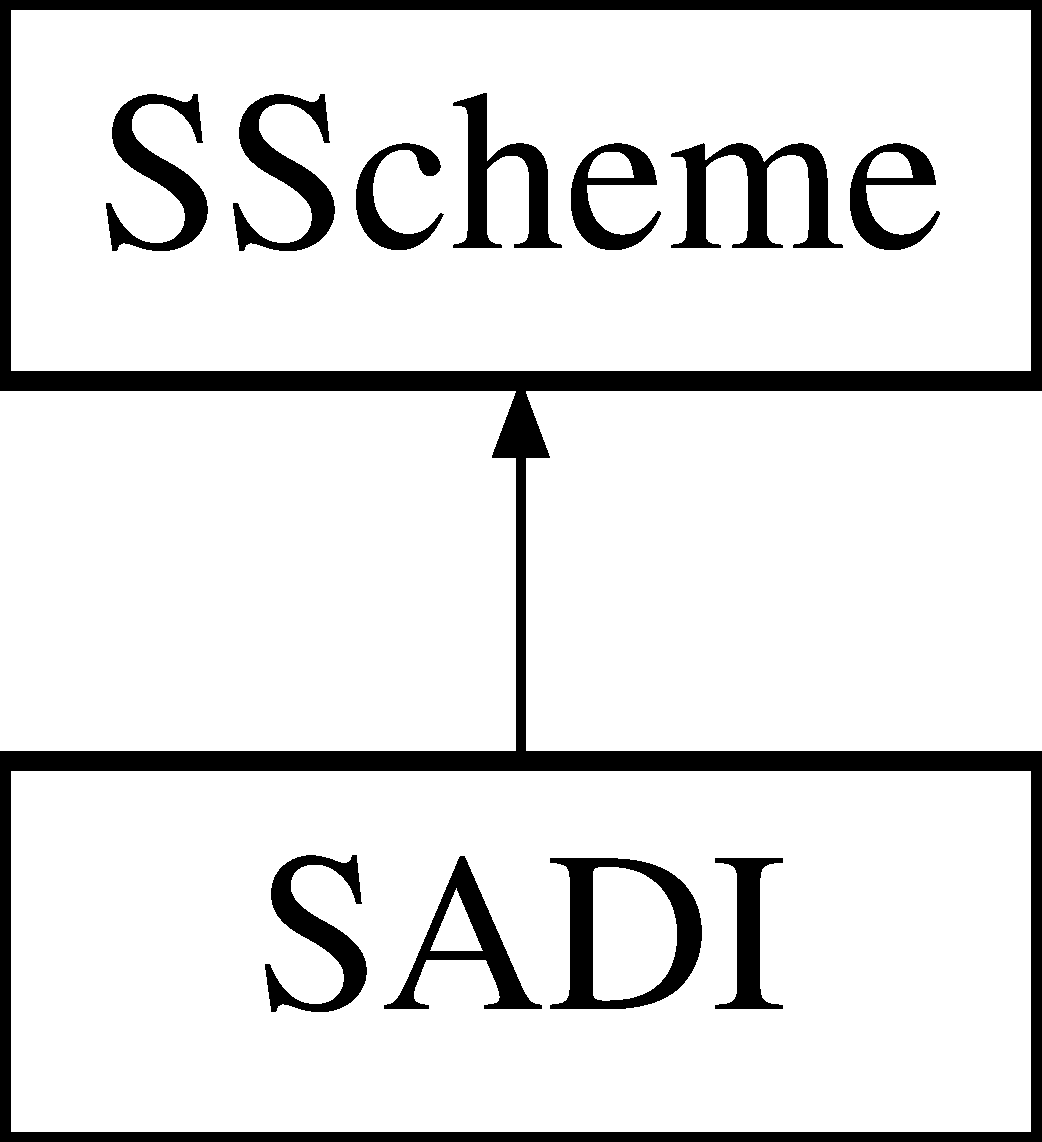
\includegraphics[height=2.000000cm]{class_s_a_d_i}
\end{center}
\end{figure}
\subsection*{Metody publiczne}
\begin{DoxyCompactItemize}
\item 
\hyperlink{class_s_a_d_i_a77c5520329e29fff358d98b9c7f323a7}{S\+A\+D\+I} ()
\begin{DoxyCompactList}\small\item\em Konstruktor. \end{DoxyCompactList}\item 
void \hyperlink{class_s_a_d_i_aed849c2b3b1a1c5b346edcfb69460457}{Compute\+Concentration} (map$<$ int, \hyperlink{class_point}{Point} $>$ \&Point\+Map)
\begin{DoxyCompactList}\small\item\em Oblicza koncentracje uzywajac schamatu A\+D\+I. \end{DoxyCompactList}\item 
void \hyperlink{class_s_a_d_i_aec6b8007d89c0c72648b4cad7aba1274}{Get\+Factors} (\hyperlink{class_point}{Point} $\ast$p, const double \&C\+Ax, const double \&C\+Ay, const double \&C\+Dx, const double \&C\+Dxy, const double \&C\+Dy, const vector$<$ int $>$ \&flag)
\end{DoxyCompactItemize}
\subsection*{Dodatkowe Dziedziczone Składowe}


\subsection{Opis szczegółowy}
Schemat naprzemiennych kierunkow A\+D\+I . 

Zawiera metody potrzebane do rozwiazania rownania transportu metoda A\+D\+I. 

Definicja w linii 283 pliku scheme.\+h.



\subsection{Dokumentacja konstruktora i destruktora}
\hypertarget{class_s_a_d_i_a77c5520329e29fff358d98b9c7f323a7}{}\index{S\+A\+D\+I@{S\+A\+D\+I}!S\+A\+D\+I@{S\+A\+D\+I}}
\index{S\+A\+D\+I@{S\+A\+D\+I}!S\+A\+D\+I@{S\+A\+D\+I}}
\subsubsection[{S\+A\+D\+I}]{\setlength{\rightskip}{0pt plus 5cm}S\+A\+D\+I\+::\+S\+A\+D\+I (
\begin{DoxyParamCaption}
{}
\end{DoxyParamCaption}
)\hspace{0.3cm}{\ttfamily [inline]}}\label{class_s_a_d_i_a77c5520329e29fff358d98b9c7f323a7}


Konstruktor. 

Tworzy schemat do rozwiazywania rownania transporu metoda A\+D\+I 

Definicja w linii 291 pliku scheme.\+h.



\subsection{Dokumentacja funkcji składowych}
\hypertarget{class_s_a_d_i_aed849c2b3b1a1c5b346edcfb69460457}{}\index{S\+A\+D\+I@{S\+A\+D\+I}!Compute\+Concentration@{Compute\+Concentration}}
\index{Compute\+Concentration@{Compute\+Concentration}!S\+A\+D\+I@{S\+A\+D\+I}}
\subsubsection[{Compute\+Concentration}]{\setlength{\rightskip}{0pt plus 5cm}void S\+A\+D\+I\+::\+Compute\+Concentration (
\begin{DoxyParamCaption}
\item[{map$<$ int, {\bf Point} $>$ \&}]{Point\+Map}
\end{DoxyParamCaption}
)\hspace{0.3cm}{\ttfamily [virtual]}}\label{class_s_a_d_i_aed849c2b3b1a1c5b346edcfb69460457}


Oblicza koncentracje uzywajac schamatu A\+D\+I. 

Oblicza koncentracje w daneym kroku uzywajac metody A\+D\+I 
\begin{DoxyParams}{Parametry}
{\em Point\+Map} & -\/ mapa punktow \\
\hline
\end{DoxyParams}
------------10.\+06.\+2015 -\/ dodajemy czlon zrodluwy

-\/-\/-\/---------10.\+06.\+2015 -\/ dodajemy czlon zrodluwy

-\/-\/-\/-\/------L\+I\+C\+Z\+E\+N\+I\+E H\+E\+A\+T F\+L\+U\+X -\/-\/-\/-\/-\/-\/-\/-\/-\/-\/-\/-\/-\/-\/------//

-\/-\/-\/-\/-\/-\/-\/---L\+I\+C\+Z\+E\+N\+I\+E H\+E\+A\+T F\+L\+U\+X -\/-\/-\/-\/-\/-\/-\/-\/-\/-\/-\/-\/-\/-\/-\/-\/-\/---// 

Reimplementowana z \hyperlink{class_s_scheme_a1607f2363ea074bde9ad9c585b5a4019}{S\+Scheme}.



Definicja w linii 1261 pliku scheme.\+cpp.

\hypertarget{class_s_a_d_i_aec6b8007d89c0c72648b4cad7aba1274}{}\index{S\+A\+D\+I@{S\+A\+D\+I}!Get\+Factors@{Get\+Factors}}
\index{Get\+Factors@{Get\+Factors}!S\+A\+D\+I@{S\+A\+D\+I}}
\subsubsection[{Get\+Factors}]{\setlength{\rightskip}{0pt plus 5cm}void S\+A\+D\+I\+::\+Get\+Factors (
\begin{DoxyParamCaption}
\item[{{\bf Point} $\ast$}]{p, }
\item[{const double \&}]{C\+Ax, }
\item[{const double \&}]{C\+Ay, }
\item[{const double \&}]{C\+Dx, }
\item[{const double \&}]{C\+Dxy, }
\item[{const double \&}]{C\+Dy, }
\item[{const vector$<$ int $>$ \&}]{flag}
\end{DoxyParamCaption}
)\hspace{0.3cm}{\ttfamily [virtual]}}\label{class_s_a_d_i_aec6b8007d89c0c72648b4cad7aba1274}
Odpowiedzilan za wyznaczenie czynnikow (a, b, c, d, e, f, g, h, i) i (fa, fb, fc, fd, fe, ff, fg, fh, fi) w rowenanie transportu dal zadanego pkt w ktorym obliczana jest koncentracja dla schemtu A\+D\+I


\begin{DoxyParams}{Parametry}
{\em $\ast$p} & -\/ pkt dla ktorego wyznaczane sa czynniki \\
\hline
{\em C\+Ax} & -\/ adwekcyjna liczba Couranta w kieruynku x \\
\hline
{\em C\+Ay} & -\/ adwekcyjna liczba Couranta w kieruynku y \\
\hline
{\em C\+Dx} & -\/ dyfuzyjna liczba Couranta w kieruynku x \\
\hline
{\em C\+Dxy} & -\/ dyfuzyjna liczba Couranta w kieruynku xy \\
\hline
{\em C\+Dy} & -\/ dyfuzyjna liczba Couranta w kieruynku y \\
\hline
\end{DoxyParams}


Reimplementowana z \hyperlink{class_s_scheme_ae1e554b35ec2d8a902f6fdb30d95ab20}{S\+Scheme}.



Definicja w linii 1387 pliku scheme.\+cpp.



Dokumentacja dla tej klasy została wygenerowana z plików\+:\begin{DoxyCompactItemize}
\item 
\hyperlink{scheme_8h}{scheme.\+h}\item 
\hyperlink{scheme_8cpp}{scheme.\+cpp}\item 
\hyperlink{scheme__new__bez_q_8cpp}{scheme\+\_\+new\+\_\+bez\+Q.\+cpp}\item 
\hyperlink{scheme__new__z_q_8cpp}{scheme\+\_\+new\+\_\+z\+Q.\+cpp}\item 
\hyperlink{scheme__przed__zmina__09092015_8cpp}{scheme\+\_\+przed\+\_\+zmina\+\_\+09092015.\+cpp}\end{DoxyCompactItemize}

\hypertarget{class_s_a_d_i2}{}\section{Dokumentacja klasy S\+A\+D\+I2}
\label{class_s_a_d_i2}\index{S\+A\+D\+I2@{S\+A\+D\+I2}}


Schemat naprzemiennych kierunkow A\+D\+I .  




{\ttfamily \#include $<$scheme.\+h$>$}

Diagram dziedziczenia dla S\+A\+D\+I2\begin{figure}[H]
\begin{center}
\leavevmode
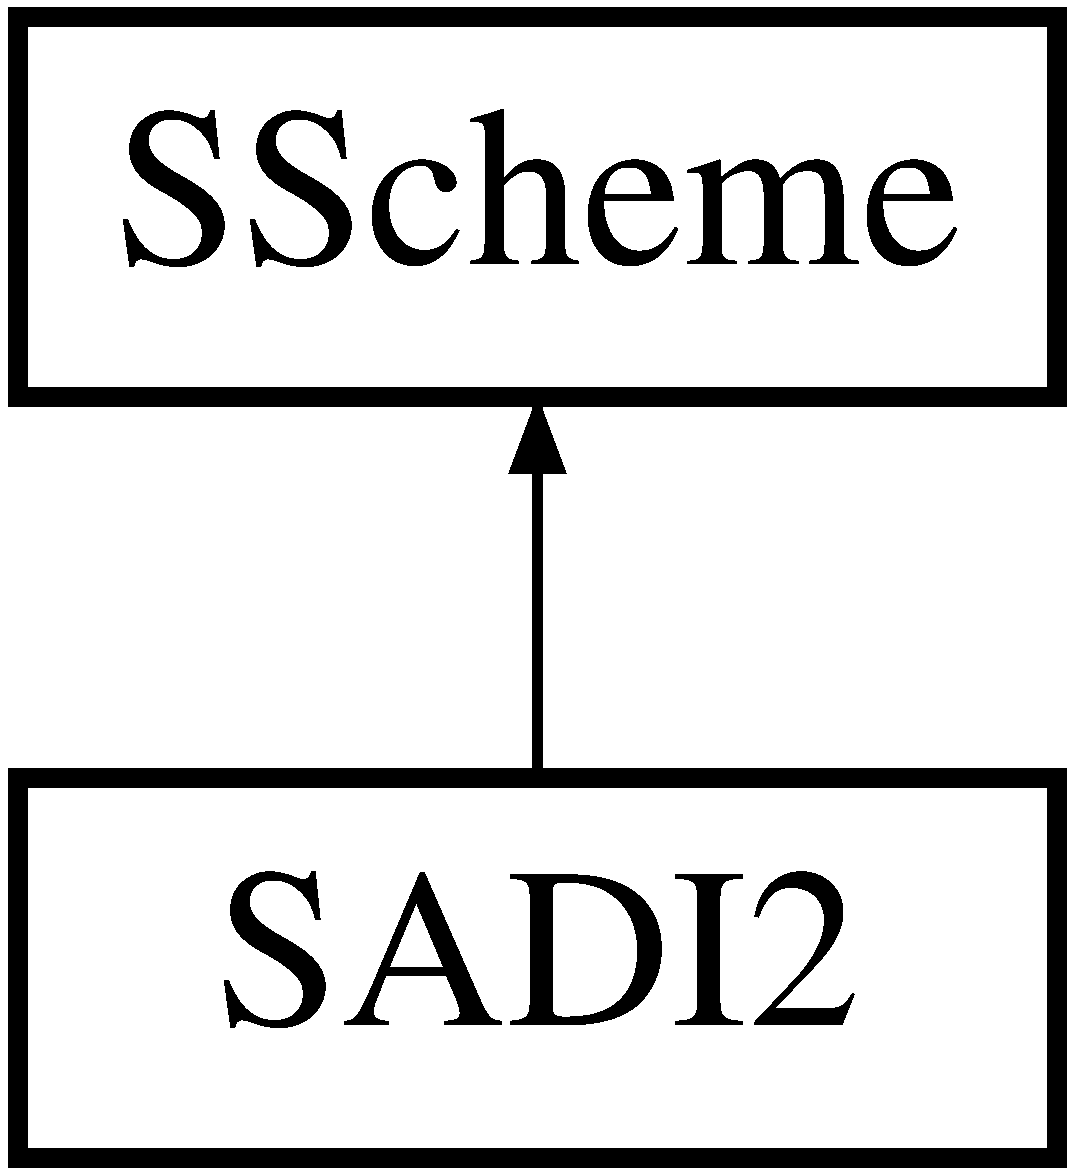
\includegraphics[height=2.000000cm]{class_s_a_d_i2}
\end{center}
\end{figure}
\subsection*{Metody publiczne}
\begin{DoxyCompactItemize}
\item 
\hyperlink{class_s_a_d_i2_ac5d404d44833aaf803fee9ae9a8d5d19}{S\+A\+D\+I2} ()
\begin{DoxyCompactList}\small\item\em Konstruktor. \end{DoxyCompactList}\item 
void \hyperlink{class_s_a_d_i2_a41903e3b443ba68fe68cbad73fe44970}{Compute\+Concentration} (map$<$ int, \hyperlink{class_point}{Point} $>$ \&Point\+Map)
\begin{DoxyCompactList}\small\item\em Oblicza koncentracje uzywajac schamatu A\+D\+I2. \end{DoxyCompactList}\item 
void \hyperlink{class_s_a_d_i2_afac90c203840a07b31f73418af815063}{Get\+Factors} (\hyperlink{class_point}{Point} $\ast$p, const double \&C\+Ax, const double \&C\+Ay, const double \&C\+Dx, const double \&C\+Dxy, const double \&C\+Dy, const vector$<$ int $>$ \&flag)
\end{DoxyCompactItemize}
\subsection*{Dodatkowe Dziedziczone Składowe}


\subsection{Opis szczegółowy}
Schemat naprzemiennych kierunkow A\+D\+I . 

Zawiera metody potrzebane do rozwiazania rownania transportu metoda A\+D\+I. 

Definicja w linii 331 pliku scheme.\+h.



\subsection{Dokumentacja konstruktora i destruktora}
\hypertarget{class_s_a_d_i2_ac5d404d44833aaf803fee9ae9a8d5d19}{}\index{S\+A\+D\+I2@{S\+A\+D\+I2}!S\+A\+D\+I2@{S\+A\+D\+I2}}
\index{S\+A\+D\+I2@{S\+A\+D\+I2}!S\+A\+D\+I2@{S\+A\+D\+I2}}
\subsubsection[{S\+A\+D\+I2}]{\setlength{\rightskip}{0pt plus 5cm}S\+A\+D\+I2\+::\+S\+A\+D\+I2 (
\begin{DoxyParamCaption}
{}
\end{DoxyParamCaption}
)\hspace{0.3cm}{\ttfamily [inline]}}\label{class_s_a_d_i2_ac5d404d44833aaf803fee9ae9a8d5d19}


Konstruktor. 

Tworzy schemat do rozwiazywania rownania transporu metoda A\+D\+I 

Definicja w linii 339 pliku scheme.\+h.



\subsection{Dokumentacja funkcji składowych}
\hypertarget{class_s_a_d_i2_a41903e3b443ba68fe68cbad73fe44970}{}\index{S\+A\+D\+I2@{S\+A\+D\+I2}!Compute\+Concentration@{Compute\+Concentration}}
\index{Compute\+Concentration@{Compute\+Concentration}!S\+A\+D\+I2@{S\+A\+D\+I2}}
\subsubsection[{Compute\+Concentration}]{\setlength{\rightskip}{0pt plus 5cm}void S\+A\+D\+I2\+::\+Compute\+Concentration (
\begin{DoxyParamCaption}
\item[{map$<$ int, {\bf Point} $>$ \&}]{Point\+Map}
\end{DoxyParamCaption}
)\hspace{0.3cm}{\ttfamily [virtual]}}\label{class_s_a_d_i2_a41903e3b443ba68fe68cbad73fe44970}


Oblicza koncentracje uzywajac schamatu A\+D\+I2. 

Oblicza koncentracje w daneym kroku uzywajac metody A\+D\+I2 (rozni sie tym od A\+D\+I1 ze ma inaczej jest podzielona na dwa \char`\"{}pdkroki\char`\"{} czasowe) 
\begin{DoxyParams}{Parametry}
{\em Point\+Map} & -\/ mapa punktow \\
\hline
\end{DoxyParams}


Reimplementowana z \hyperlink{class_s_scheme_a1607f2363ea074bde9ad9c585b5a4019}{S\+Scheme}.



Definicja w linii 1699 pliku scheme.\+cpp.

\hypertarget{class_s_a_d_i2_afac90c203840a07b31f73418af815063}{}\index{S\+A\+D\+I2@{S\+A\+D\+I2}!Get\+Factors@{Get\+Factors}}
\index{Get\+Factors@{Get\+Factors}!S\+A\+D\+I2@{S\+A\+D\+I2}}
\subsubsection[{Get\+Factors}]{\setlength{\rightskip}{0pt plus 5cm}void S\+A\+D\+I2\+::\+Get\+Factors (
\begin{DoxyParamCaption}
\item[{{\bf Point} $\ast$}]{p, }
\item[{const double \&}]{C\+Ax, }
\item[{const double \&}]{C\+Ay, }
\item[{const double \&}]{C\+Dx, }
\item[{const double \&}]{C\+Dxy, }
\item[{const double \&}]{C\+Dy, }
\item[{const vector$<$ int $>$ \&}]{flag}
\end{DoxyParamCaption}
)\hspace{0.3cm}{\ttfamily [virtual]}}\label{class_s_a_d_i2_afac90c203840a07b31f73418af815063}
Odpowiedzilan za wyznaczenie czynnikow (a, b, c, d, e, f, g, h, i) i (fa, fb, fc, fd, fe, ff, fg, fh, fi) w rowenanie transportu dal zadanego pkt w ktorym obliczana jest koncentracja dla schemtu A\+D\+I2


\begin{DoxyParams}{Parametry}
{\em $\ast$p} & -\/ pkt dla ktorego wyznaczane sa czynniki \\
\hline
{\em C\+Ax} & -\/ adwekcyjna liczba Couranta w kieruynku x \\
\hline
{\em C\+Ay} & -\/ adwekcyjna liczba Couranta w kieruynku y \\
\hline
{\em C\+Dx} & -\/ dyfuzyjna liczba Couranta w kieruynku x \\
\hline
{\em C\+Dxy} & -\/ dyfuzyjna liczba Couranta w kieruynku xy \\
\hline
{\em C\+Dy} & -\/ dyfuzyjna liczba Couranta w kieruynku y \\
\hline
\end{DoxyParams}


Reimplementowana z \hyperlink{class_s_scheme_ae1e554b35ec2d8a902f6fdb30d95ab20}{S\+Scheme}.



Definicja w linii 1894 pliku scheme.\+cpp.



Dokumentacja dla tej klasy została wygenerowana z plików\+:\begin{DoxyCompactItemize}
\item 
\hyperlink{scheme_8h}{scheme.\+h}\item 
\hyperlink{scheme_8cpp}{scheme.\+cpp}\item 
\hyperlink{scheme__new__bez_q_8cpp}{scheme\+\_\+new\+\_\+bez\+Q.\+cpp}\item 
\hyperlink{scheme__new__z_q_8cpp}{scheme\+\_\+new\+\_\+z\+Q.\+cpp}\item 
\hyperlink{scheme__przed__zmina__09092015_8cpp}{scheme\+\_\+przed\+\_\+zmina\+\_\+09092015.\+cpp}\end{DoxyCompactItemize}

\hypertarget{class_s_crank_nicolson}{}\section{Dokumentacja klasy S\+Crank\+Nicolson}
\label{class_s_crank_nicolson}\index{S\+Crank\+Nicolson@{S\+Crank\+Nicolson}}


Schemat Cranka Nicolsona.  




{\ttfamily \#include $<$scheme.\+h$>$}

Diagram dziedziczenia dla S\+Crank\+Nicolson\begin{figure}[H]
\begin{center}
\leavevmode
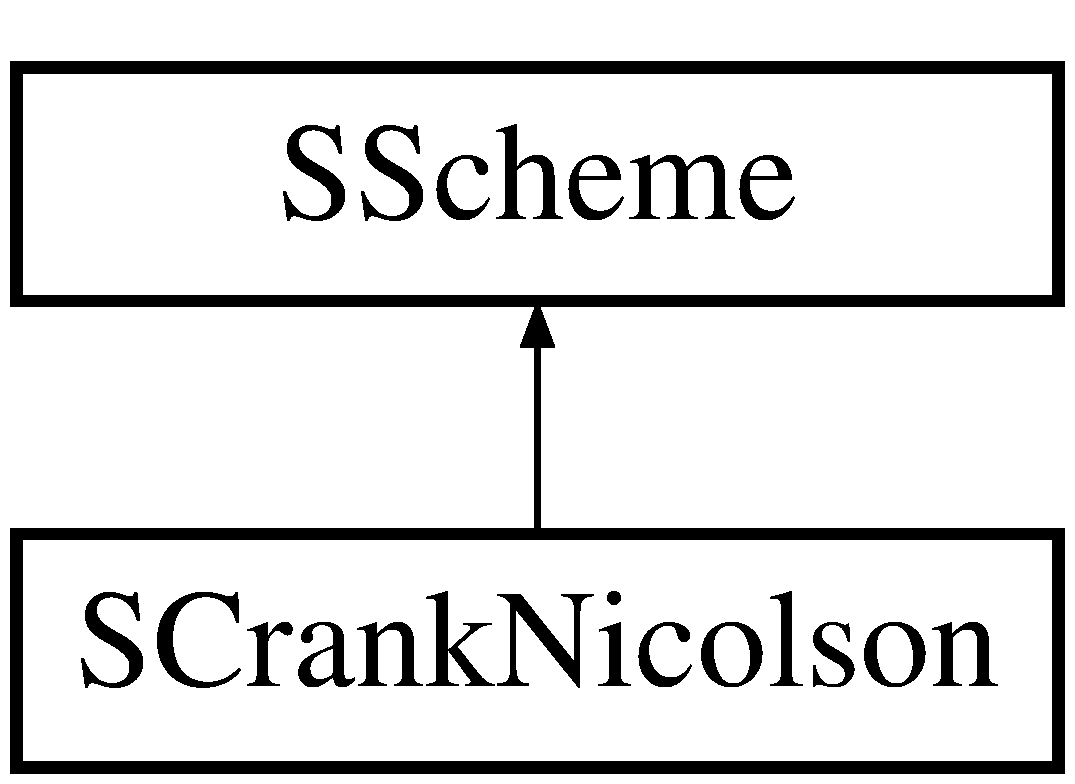
\includegraphics[height=2.000000cm]{class_s_crank_nicolson}
\end{center}
\end{figure}
\subsection*{Metody publiczne}
\begin{DoxyCompactItemize}
\item 
\hyperlink{class_s_crank_nicolson_a914a9f8786b91fd4ceae1a9f0e99cff8}{S\+Crank\+Nicolson} ()
\begin{DoxyCompactList}\small\item\em Konstruktor. \end{DoxyCompactList}\item 
void \hyperlink{class_s_crank_nicolson_abe37e0a2d5078a17420b3e9d815fc85f}{Compute\+Concentration} (map$<$ int, \hyperlink{class_point}{Point} $>$ \&Point\+Map)
\begin{DoxyCompactList}\small\item\em Oblicza koncentracje uzywajac schamatu Cranka Nicolsona. \end{DoxyCompactList}\item 
void \hyperlink{class_s_crank_nicolson_a1fd8e8aee2c7fb9f61e6c4b02b74e1b3}{Get\+Factors} (\hyperlink{class_point}{Point} $\ast$p, const double \&C\+Ax, const double \&C\+Ay, const double \&C\+Dx, const double \&C\+Dxy, const double \&C\+Dy, const vector$<$ int $>$ \&flag)
\end{DoxyCompactItemize}
\subsection*{Dodatkowe Dziedziczone Składowe}


\subsection{Opis szczegółowy}
Schemat Cranka Nicolsona. 

Zawiera metody potrzebane do rozwiazania rownania transportu metoda Crnka Nicolsona. 

Definicja w linii 193 pliku scheme.\+h.



\subsection{Dokumentacja konstruktora i destruktora}
\hypertarget{class_s_crank_nicolson_a914a9f8786b91fd4ceae1a9f0e99cff8}{}\index{S\+Crank\+Nicolson@{S\+Crank\+Nicolson}!S\+Crank\+Nicolson@{S\+Crank\+Nicolson}}
\index{S\+Crank\+Nicolson@{S\+Crank\+Nicolson}!S\+Crank\+Nicolson@{S\+Crank\+Nicolson}}
\subsubsection[{S\+Crank\+Nicolson}]{\setlength{\rightskip}{0pt plus 5cm}S\+Crank\+Nicolson\+::\+S\+Crank\+Nicolson (
\begin{DoxyParamCaption}
{}
\end{DoxyParamCaption}
)\hspace{0.3cm}{\ttfamily [inline]}}\label{class_s_crank_nicolson_a914a9f8786b91fd4ceae1a9f0e99cff8}


Konstruktor. 

Tworzy schemat do rozwiazywania rownania transporu metoda Cranka Nicolsona 

Definicja w linii 201 pliku scheme.\+h.



\subsection{Dokumentacja funkcji składowych}
\hypertarget{class_s_crank_nicolson_abe37e0a2d5078a17420b3e9d815fc85f}{}\index{S\+Crank\+Nicolson@{S\+Crank\+Nicolson}!Compute\+Concentration@{Compute\+Concentration}}
\index{Compute\+Concentration@{Compute\+Concentration}!S\+Crank\+Nicolson@{S\+Crank\+Nicolson}}
\subsubsection[{Compute\+Concentration}]{\setlength{\rightskip}{0pt plus 5cm}void S\+Crank\+Nicolson\+::\+Compute\+Concentration (
\begin{DoxyParamCaption}
\item[{map$<$ int, {\bf Point} $>$ \&}]{Point\+Map}
\end{DoxyParamCaption}
)\hspace{0.3cm}{\ttfamily [virtual]}}\label{class_s_crank_nicolson_abe37e0a2d5078a17420b3e9d815fc85f}


Oblicza koncentracje uzywajac schamatu Cranka Nicolsona. 

Oblicza koncentracje w daneym kroku uzywajac metody Cranka Nicolsona 
\begin{DoxyParams}{Parametry}
{\em Point\+Map} & -\/ mapa punktow \\
\hline
\end{DoxyParams}


Reimplementowana z \hyperlink{class_s_scheme_a1607f2363ea074bde9ad9c585b5a4019}{S\+Scheme}.



Definicja w linii 382 pliku scheme.\+cpp.

\hypertarget{class_s_crank_nicolson_a1fd8e8aee2c7fb9f61e6c4b02b74e1b3}{}\index{S\+Crank\+Nicolson@{S\+Crank\+Nicolson}!Get\+Factors@{Get\+Factors}}
\index{Get\+Factors@{Get\+Factors}!S\+Crank\+Nicolson@{S\+Crank\+Nicolson}}
\subsubsection[{Get\+Factors}]{\setlength{\rightskip}{0pt plus 5cm}void S\+Crank\+Nicolson\+::\+Get\+Factors (
\begin{DoxyParamCaption}
\item[{{\bf Point} $\ast$}]{p, }
\item[{const double \&}]{C\+Ax, }
\item[{const double \&}]{C\+Ay, }
\item[{const double \&}]{C\+Dx, }
\item[{const double \&}]{C\+Dxy, }
\item[{const double \&}]{C\+Dy, }
\item[{const vector$<$ int $>$ \&}]{flag}
\end{DoxyParamCaption}
)\hspace{0.3cm}{\ttfamily [virtual]}}\label{class_s_crank_nicolson_a1fd8e8aee2c7fb9f61e6c4b02b74e1b3}
Odpowiedzilan za wyznaczenie czynnikow (a, b, c, d, e, f, g, h, i) i (fa, fb, fc, fd, fe, ff, fg, fh, fi) w rowenanie transportu dal zadanego pkt w ktorym obliczana jest koncentracja dla schemtau Cranka Nicolsona


\begin{DoxyParams}{Parametry}
{\em $\ast$p} & -\/ pkt dla ktorego wyznaczane sa czynniki \\
\hline
{\em C\+Ax} & -\/ adwekcyjna liczba Couranta w kieruynku x \\
\hline
{\em C\+Ay} & -\/ adwekcyjna liczba Couranta w kieruynku y \\
\hline
{\em C\+Dx} & -\/ dyfuzyjna liczba Couranta w kieruynku x \\
\hline
{\em C\+Dxy} & -\/ dyfuzyjna liczba Couranta w kieruynku xy \\
\hline
{\em C\+Dy} & -\/ dyfuzyjna liczba Couranta w kieruynku y \\
\hline
\end{DoxyParams}


Reimplementowana z \hyperlink{class_s_scheme_ae1e554b35ec2d8a902f6fdb30d95ab20}{S\+Scheme}.



Definicja w linii 426 pliku scheme.\+cpp.



Dokumentacja dla tej klasy została wygenerowana z plików\+:\begin{DoxyCompactItemize}
\item 
\hyperlink{scheme_8h}{scheme.\+h}\item 
\hyperlink{scheme_8cpp}{scheme.\+cpp}\item 
\hyperlink{scheme__new__bez_q_8cpp}{scheme\+\_\+new\+\_\+bez\+Q.\+cpp}\item 
\hyperlink{scheme__new__z_q_8cpp}{scheme\+\_\+new\+\_\+z\+Q.\+cpp}\item 
\hyperlink{scheme__przed__zmina__09092015_8cpp}{scheme\+\_\+przed\+\_\+zmina\+\_\+09092015.\+cpp}\end{DoxyCompactItemize}

\hypertarget{class_simulation}{}\section{Dokumentacja klasy Simulation}
\label{class_simulation}\index{Simulation@{Simulation}}


Klasa odpowiedzialna za symulacje.  




{\ttfamily \#include $<$simulation.\+h$>$}

\subsection*{Metody publiczne}
\begin{DoxyCompactItemize}
\item 
\hyperlink{class_simulation_af6d6faabf99b4147db641658d1fcfc08}{Simulation} (const string \&param\+File, const string \&save\+File)
\begin{DoxyCompactList}\small\item\em Konstruktor. \end{DoxyCompactList}\item 
void \hyperlink{class_simulation_a900ea19845f934638b3e2cf755e14302}{My\+Simulation} (const string \&param\+\_\+file, const string \&save\+\_\+file)
\item 
int \hyperlink{class_simulation_ab76ff3b4cdd23182a21a69535c4b064b}{Set\+Param} (\hyperlink{class_simulation_parameters}{Simulation\+Parameters} $\ast$param, const string \&file)
\item 
int \hyperlink{class_simulation_a7f0f2ce0a990c9823748cee649224bfc}{Prepare\+Map} (map$<$ int, \hyperlink{class_point}{Point} $>$ \&Point\+Map, \hyperlink{class_simulation_parameters}{Simulation\+Parameters} \&param)
\item 
int \hyperlink{class_simulation_a01d0cc9ca7a6b8bb20504b0d303c077a}{Set\+Save\+Parameters} (const string \&file, int n)
\begin{DoxyCompactList}\small\item\em Odczytuje z pliku i ustawia parametry zapisu wyników symulacji. \end{DoxyCompactList}\item 
void \hyperlink{class_simulation_a471316287d132dba2d8dd10fbcc1a192}{Save\+Map} (map$<$ int, \hyperlink{class_point}{Point} $>$ \&Point\+Map, const string \&file, const string \&opt)
\item 
void \hyperlink{class_simulation_ac9b7432d7f91aaee99100187fac8d73e}{Set\+Source\+Concentration} (map$<$ int, \hyperlink{class_point}{Point} $>$ \&Point\+Map, double \&val)
\item 
void \hyperlink{class_simulation_ad8c565d908664e7b5d419261af556ae9}{Set\+Source\+Concentration\+Temp} (map$<$ int, \hyperlink{class_point}{Point} $>$ \&Point\+Map, \hyperlink{class_simulation_parameters}{Simulation\+Parameters} \&param, double \&val)
\item 
double \hyperlink{class_simulation_a9bd641b3fd013d152d03b5b5ea718d73}{Compute\+Effective\+Temp} (\hyperlink{class_point}{Point} \&p, double dx, double val, double hz=-\/9999.\+99, double Qz=-\/9999.\+99)
\item 
int \hyperlink{class_simulation_a3253bdc42110ee6653d7f02a420b56af}{Set\+Initial\+Concentration} (map$<$ int, \hyperlink{class_point}{Point} $>$ \&Point\+Map, \hyperlink{class_simulation_parameters}{Simulation\+Parameters} \&param)
\item 
void \hyperlink{class_simulation_ae713b7bd19b86d3e426c899785b9ce8a}{Set\+Initial\+Concentration\+Point} (map$<$ int, \hyperlink{class_point}{Point} $>$ \&Point\+Map, \hyperlink{class_simulation_parameters}{Simulation\+Parameters} \&param, double x0, double y0, double val)
\item 
void \hyperlink{class_simulation_a41155db84b2177e858dfd8274a9a4a93}{Set\+Initial\+Concentration\+Plane\+Wave} (map$<$ int, \hyperlink{class_point}{Point} $>$ \&Point\+Map)
\item 
void \hyperlink{class_simulation_aed95dfa701b563cbd85421bfeb4f74fd}{Set\+Initial\+Concentration\+Gauss} (map$<$ int, \hyperlink{class_point}{Point} $>$ \&Point\+Map, \hyperlink{class_simulation_parameters}{Simulation\+Parameters} \&param, double x0, double y0, double val, int krok)
\item 
void \hyperlink{class_simulation_a4f95080d3efd1568155f493150ea6a5e}{Set\+Initial\+Concentration\+Gauss\+Non\+Diag} (map$<$ int, \hyperlink{class_point}{Point} $>$ \&Point\+Map, \hyperlink{class_simulation_parameters}{Simulation\+Parameters} \&param, double x0, double y0, double val, int krok)
\item 
double \hyperlink{class_simulation_a99e94c6106312a2e741e4a7fbfc17acc}{Gaus} (double x, double mean, double sigma, bool norm)
\item 
int \hyperlink{class_simulation_a63da2c122d167f06255071009070f0b2}{Set\+Initial\+Concentration\+File} (map$<$ int, \hyperlink{class_point}{Point} $>$ \&Point\+Map)
\item 
void \hyperlink{class_simulation_a404b11e725f52fc7e87986956229fa38}{Set\+In\+Out\+Point\+Value} (map$<$ int, \hyperlink{class_point}{Point} $>$ \&Point\+Map)
\item 
double \hyperlink{class_simulation_affeb8b328bfd85259dfd4942591a3210}{My\+\_\+\+Gaus} (double x, double y, double mean\+X, double mean\+Y, double sigma)
\item 
void \hyperlink{class_simulation_ac9e2c2d48ff778482992d64ec3d63f60}{set\+\_\+file} (string file)
\item 
string \hyperlink{class_simulation_af8e26312c6ff919274ca640abe83bca2}{get\+\_\+file} () const 
\item 
double \hyperlink{class_simulation_a7a0437249ae44f92299590cf7fbdb7bd}{Compute\+Effective\+Temp} (\hyperlink{class_point}{Point} pkt, double arg2, double arg3, double val1, double hz, double Qz)
\end{DoxyCompactItemize}


\subsection{Opis szczegółowy}
Klasa odpowiedzialna za symulacje. 

Odpowiedizlna za przygotowanie danych do symulacji start i przebieg symulacji 

Definicja w linii 35 pliku simulation.\+h.



\subsection{Dokumentacja konstruktora i destruktora}
\hypertarget{class_simulation_af6d6faabf99b4147db641658d1fcfc08}{}\index{Simulation@{Simulation}!Simulation@{Simulation}}
\index{Simulation@{Simulation}!Simulation@{Simulation}}
\subsubsection[{Simulation}]{\setlength{\rightskip}{0pt plus 5cm}Simulation\+::\+Simulation (
\begin{DoxyParamCaption}
\item[{const string \&}]{param\+File, }
\item[{const string \&}]{save\+File}
\end{DoxyParamCaption}
)}\label{class_simulation_af6d6faabf99b4147db641658d1fcfc08}


Konstruktor. 

Tworzy obiekt simuation 
\begin{DoxyParams}{Parametry}
{\em param\+File} & -\/ nazwa pliku z parametrami symulacji \\
\hline
{\em save\+File} & -\/ nazwa pliku z parametrami zapisu wyników symulacji \\
\hline
\end{DoxyParams}


Definicja w linii 15 pliku simulation.\+cpp.



\subsection{Dokumentacja funkcji składowych}
\hypertarget{class_simulation_a9bd641b3fd013d152d03b5b5ea718d73}{}\index{Simulation@{Simulation}!Compute\+Effective\+Temp@{Compute\+Effective\+Temp}}
\index{Compute\+Effective\+Temp@{Compute\+Effective\+Temp}!Simulation@{Simulation}}
\subsubsection[{Compute\+Effective\+Temp}]{\setlength{\rightskip}{0pt plus 5cm}double Simulation\+::\+Compute\+Effective\+Temp (
\begin{DoxyParamCaption}
\item[{{\bf Point} \&}]{p, }
\item[{double}]{dx, }
\item[{double}]{val, }
\item[{double}]{hz = {\ttfamily -\/9999.99}, }
\item[{double}]{Qz = {\ttfamily -\/9999.99}}
\end{DoxyParamCaption}
)}\label{class_simulation_a9bd641b3fd013d152d03b5b5ea718d73}


Definicja w linii 936 pliku simulation.\+cpp.

\hypertarget{class_simulation_a7a0437249ae44f92299590cf7fbdb7bd}{}\index{Simulation@{Simulation}!Compute\+Effective\+Temp@{Compute\+Effective\+Temp}}
\index{Compute\+Effective\+Temp@{Compute\+Effective\+Temp}!Simulation@{Simulation}}
\subsubsection[{Compute\+Effective\+Temp}]{\setlength{\rightskip}{0pt plus 5cm}double Simulation\+::\+Compute\+Effective\+Temp (
\begin{DoxyParamCaption}
\item[{{\bf Point}}]{pkt, }
\item[{double}]{arg2, }
\item[{double}]{arg3, }
\item[{double}]{val1, }
\item[{double}]{hz, }
\item[{double}]{Qz}
\end{DoxyParamCaption}
)}\label{class_simulation_a7a0437249ae44f92299590cf7fbdb7bd}
\hypertarget{class_simulation_a99e94c6106312a2e741e4a7fbfc17acc}{}\index{Simulation@{Simulation}!Gaus@{Gaus}}
\index{Gaus@{Gaus}!Simulation@{Simulation}}
\subsubsection[{Gaus}]{\setlength{\rightskip}{0pt plus 5cm}double Simulation\+::\+Gaus (
\begin{DoxyParamCaption}
\item[{double}]{x, }
\item[{double}]{mean, }
\item[{double}]{sigma, }
\item[{bool}]{norm}
\end{DoxyParamCaption}
)}\label{class_simulation_a99e94c6106312a2e741e4a7fbfc17acc}


Definicja w linii 768 pliku simulation.\+cpp.

\hypertarget{class_simulation_af8e26312c6ff919274ca640abe83bca2}{}\index{Simulation@{Simulation}!get\+\_\+file@{get\+\_\+file}}
\index{get\+\_\+file@{get\+\_\+file}!Simulation@{Simulation}}
\subsubsection[{get\+\_\+file}]{\setlength{\rightskip}{0pt plus 5cm}string Simulation\+::get\+\_\+file (
\begin{DoxyParamCaption}
{}
\end{DoxyParamCaption}
) const\hspace{0.3cm}{\ttfamily [inline]}}\label{class_simulation_af8e26312c6ff919274ca640abe83bca2}


Definicja w linii 176 pliku simulation.\+h.

\hypertarget{class_simulation_affeb8b328bfd85259dfd4942591a3210}{}\index{Simulation@{Simulation}!My\+\_\+\+Gaus@{My\+\_\+\+Gaus}}
\index{My\+\_\+\+Gaus@{My\+\_\+\+Gaus}!Simulation@{Simulation}}
\subsubsection[{My\+\_\+\+Gaus}]{\setlength{\rightskip}{0pt plus 5cm}double Simulation\+::\+My\+\_\+\+Gaus (
\begin{DoxyParamCaption}
\item[{double}]{x, }
\item[{double}]{y, }
\item[{double}]{mean\+X, }
\item[{double}]{mean\+Y, }
\item[{double}]{sigma}
\end{DoxyParamCaption}
)}\label{class_simulation_affeb8b328bfd85259dfd4942591a3210}


Definicja w linii 925 pliku simulation.\+cpp.

\hypertarget{class_simulation_a900ea19845f934638b3e2cf755e14302}{}\index{Simulation@{Simulation}!My\+Simulation@{My\+Simulation}}
\index{My\+Simulation@{My\+Simulation}!Simulation@{Simulation}}
\subsubsection[{My\+Simulation}]{\setlength{\rightskip}{0pt plus 5cm}void Simulation\+::\+My\+Simulation (
\begin{DoxyParamCaption}
\item[{const string \&}]{param\+\_\+file, }
\item[{const string \&}]{save\+\_\+file}
\end{DoxyParamCaption}
)}\label{class_simulation_a900ea19845f934638b3e2cf755e14302}
Przebieg symulacji od ustawienia parametrow przez uruchominie obiczen po zapis danych i zakonczenie double val = 2.\+0; //wisla, ekspertyza dla kroku dx =10, na krotkim odcinku 

Definicja w linii 23 pliku simulation.\+cpp.

\hypertarget{class_simulation_a7f0f2ce0a990c9823748cee649224bfc}{}\index{Simulation@{Simulation}!Prepare\+Map@{Prepare\+Map}}
\index{Prepare\+Map@{Prepare\+Map}!Simulation@{Simulation}}
\subsubsection[{Prepare\+Map}]{\setlength{\rightskip}{0pt plus 5cm}int Simulation\+::\+Prepare\+Map (
\begin{DoxyParamCaption}
\item[{map$<$ int, {\bf Point} $>$ \&}]{Point\+Map, }
\item[{{\bf Simulation\+Parameters} \&}]{param}
\end{DoxyParamCaption}
)}\label{class_simulation_a7f0f2ce0a990c9823748cee649224bfc}
Przygotowuje Mape Punktow (siatke) na ktorej bedize przeprowadona symulacja 
\begin{DoxyParams}{Parametry}
{\em Point\+Map} & -\/ pusta mapa \\
\hline
{\em param} & -\/ obiekt z parametrami symulacji \\
\hline
\end{DoxyParams}


Definicja w linii 196 pliku simulation.\+cpp.

\hypertarget{class_simulation_a471316287d132dba2d8dd10fbcc1a192}{}\index{Simulation@{Simulation}!Save\+Map@{Save\+Map}}
\index{Save\+Map@{Save\+Map}!Simulation@{Simulation}}
\subsubsection[{Save\+Map}]{\setlength{\rightskip}{0pt plus 5cm}void Simulation\+::\+Save\+Map (
\begin{DoxyParamCaption}
\item[{map$<$ int, {\bf Point} $>$ \&}]{Point\+Map, }
\item[{const string \&}]{file, }
\item[{const string \&}]{opt}
\end{DoxyParamCaption}
)}\label{class_simulation_a471316287d132dba2d8dd10fbcc1a192}
zapisueje Mape Punktow do podanego pliku 
\begin{DoxyParams}{Parametry}
{\em Point\+Map} & -\/ mapa pkt \\
\hline
{\em file} & -\/ nazwa pliku do ktorego ma byc zapisana mapa punktow \\
\hline
{\em opt} & -\/ opcja wskazujaca co mam byc zapisane 
\begin{DoxyItemize}
\item all -\/ zapisuje wszystkie dostepne wartosci dla kazdego pkt 
\item grid -\/ zapisuje tylko siatke pkt (wpolrzedne x, y pktow i ich flagi)  
\end{DoxyItemize}\\
\hline
\end{DoxyParams}


Definicja w linii 356 pliku simulation.\+cpp.

\hypertarget{class_simulation_ac9e2c2d48ff778482992d64ec3d63f60}{}\index{Simulation@{Simulation}!set\+\_\+file@{set\+\_\+file}}
\index{set\+\_\+file@{set\+\_\+file}!Simulation@{Simulation}}
\subsubsection[{set\+\_\+file}]{\setlength{\rightskip}{0pt plus 5cm}void Simulation\+::set\+\_\+file (
\begin{DoxyParamCaption}
\item[{string}]{file}
\end{DoxyParamCaption}
)\hspace{0.3cm}{\ttfamily [inline]}}\label{class_simulation_ac9e2c2d48ff778482992d64ec3d63f60}


Definicja w linii 175 pliku simulation.\+h.

\hypertarget{class_simulation_a3253bdc42110ee6653d7f02a420b56af}{}\index{Simulation@{Simulation}!Set\+Initial\+Concentration@{Set\+Initial\+Concentration}}
\index{Set\+Initial\+Concentration@{Set\+Initial\+Concentration}!Simulation@{Simulation}}
\subsubsection[{Set\+Initial\+Concentration}]{\setlength{\rightskip}{0pt plus 5cm}void Simulation\+::\+Set\+Initial\+Concentration (
\begin{DoxyParamCaption}
\item[{map$<$ int, {\bf Point} $>$ \&}]{Point\+Map, }
\item[{{\bf Simulation\+Parameters} \&}]{param}
\end{DoxyParamCaption}
)}\label{class_simulation_a3253bdc42110ee6653d7f02a420b56af}
Wczytuje dane z pliku  \char`\"{}ini\+\_\+cond.\+txt\char`\"{} dotyczące wartości początkowej koncentracji/temperatury i wywołuje właściwą funckcję zająca wartosci koncentracji/temperatur początkowej na siatce 
\begin{DoxyParams}{Parametry}
{\em Point\+Map} & -\/ pusta mapa \\
\hline
{\em param} & -\/ obiekt z parametrami symulacji ~\newline
\\
\hline
\end{DoxyParams}
format pliku {\ttfamily \char`\"{}ini\+\_\+cond.\+txt\char`\"{}} \+:~\newline
 -\/-\/-\/-\/-\/-\/-\/-\/-\/-\/-\/-\/-\/-\/-\/-\/-\/-\/-\/-\/-\/-\/-\/-\/-\/-\/-\/-\/-\/-\/-\/-\/-\/-\/-\/-\/-\/-\/--- ~\newline
 \hyperlink{class_simulation_parameters_a76420499d58b303411f21c385d82303f}{pollutant} ~\newline
 \hyperlink{class_simulation_parameters_a1848a63487254ccce60bc06886d29847}{dump} ~\newline
 \hyperlink{class_simulation_parameters_a05862812dec3b947f124886aaea1cb84}{area} ~\newline
 \hyperlink{class_simulation_parameters_a16d7b0beff55cf45ca7cf23d99fbbd10}{mod} $x$ $y$ $val$ $h_{z}$ $Q_{z}$ ~\newline
 \hyperlink{class_simulation_parameters_a16d7b0beff55cf45ca7cf23d99fbbd10}{mod} $x$ $y$ $val$ $h_{z}$ $Q_{z}$ ~\newline
 ...~\newline
 \hyperlink{class_simulation_parameters_a16d7b0beff55cf45ca7cf23d99fbbd10}{mod} $x$ $y$ $val$ $h_{z}$ $Q_{z}$ ~\newline
 -\/-\/-\/-\/-\/-\/-\/-\/-\/-\/-\/-\/-\/-\/-\/-\/-\/-\/-\/-\/-\/-\/-\/-\/-\/-\/-\/-\/-\/-\/-\/-\/-\/-\/-\/-\/-\/-\/--- ~\newline
 Kliknij na zmienną aby zoabczyć możliwe wartości~\newline
 $x$ $y$ -\/ współrzędne punktu lokalizacji źródła ~\newline
 jeśli mod == val $h_{z}$ $Q_{z}$ -\/ wartości głebokości oraz natężenia przepływu w miejscu źródła ~\newline
 $val$ -\/ wartość koncentracji/temperatury w miejscu źródła\textbackslash{} Można podać wiele punktów w kolejnych liniach !!!!! zrobic by bylo to czytane z pliku 

Definicja w linii 950 pliku simulation.\+cpp.

\hypertarget{class_simulation_a63da2c122d167f06255071009070f0b2}{}\index{Simulation@{Simulation}!Set\+Initial\+Concentration\+File@{Set\+Initial\+Concentration\+File}}
\index{Set\+Initial\+Concentration\+File@{Set\+Initial\+Concentration\+File}!Simulation@{Simulation}}
\subsubsection[{Set\+Initial\+Concentration\+File}]{\setlength{\rightskip}{0pt plus 5cm}int Simulation\+::\+Set\+Initial\+Concentration\+File (
\begin{DoxyParamCaption}
\item[{map$<$ int, {\bf Point} $>$ \&}]{Point\+Map}
\end{DoxyParamCaption}
)}\label{class_simulation_a63da2c122d167f06255071009070f0b2}
\hypertarget{class_simulation_aed95dfa701b563cbd85421bfeb4f74fd}{}\index{Simulation@{Simulation}!Set\+Initial\+Concentration\+Gauss@{Set\+Initial\+Concentration\+Gauss}}
\index{Set\+Initial\+Concentration\+Gauss@{Set\+Initial\+Concentration\+Gauss}!Simulation@{Simulation}}
\subsubsection[{Set\+Initial\+Concentration\+Gauss}]{\setlength{\rightskip}{0pt plus 5cm}void Simulation\+::\+Set\+Initial\+Concentration\+Gauss (
\begin{DoxyParamCaption}
\item[{map$<$ int, {\bf Point} $>$ \&}]{Point\+Map, }
\item[{{\bf Simulation\+Parameters} \&}]{param, }
\item[{double}]{x0, }
\item[{double}]{y0, }
\item[{double}]{val, }
\item[{int}]{krok}
\end{DoxyParamCaption}
)}\label{class_simulation_aed95dfa701b563cbd85421bfeb4f74fd}


Definicja w linii 703 pliku simulation.\+cpp.

\hypertarget{class_simulation_a4f95080d3efd1568155f493150ea6a5e}{}\index{Simulation@{Simulation}!Set\+Initial\+Concentration\+Gauss\+Non\+Diag@{Set\+Initial\+Concentration\+Gauss\+Non\+Diag}}
\index{Set\+Initial\+Concentration\+Gauss\+Non\+Diag@{Set\+Initial\+Concentration\+Gauss\+Non\+Diag}!Simulation@{Simulation}}
\subsubsection[{Set\+Initial\+Concentration\+Gauss\+Non\+Diag}]{\setlength{\rightskip}{0pt plus 5cm}void Simulation\+::\+Set\+Initial\+Concentration\+Gauss\+Non\+Diag (
\begin{DoxyParamCaption}
\item[{map$<$ int, {\bf Point} $>$ \&}]{Point\+Map, }
\item[{{\bf Simulation\+Parameters} \&}]{param, }
\item[{double}]{x0, }
\item[{double}]{y0, }
\item[{double}]{val, }
\item[{int}]{krok}
\end{DoxyParamCaption}
)}\label{class_simulation_a4f95080d3efd1568155f493150ea6a5e}
!!! double norm = 4$\ast$pi$\ast$krok$\ast$dt$\ast$sqrt(D); 

Definicja w linii 785 pliku simulation.\+cpp.

\hypertarget{class_simulation_a41155db84b2177e858dfd8274a9a4a93}{}\index{Simulation@{Simulation}!Set\+Initial\+Concentration\+Plane\+Wave@{Set\+Initial\+Concentration\+Plane\+Wave}}
\index{Set\+Initial\+Concentration\+Plane\+Wave@{Set\+Initial\+Concentration\+Plane\+Wave}!Simulation@{Simulation}}
\subsubsection[{Set\+Initial\+Concentration\+Plane\+Wave}]{\setlength{\rightskip}{0pt plus 5cm}void Simulation\+::\+Set\+Initial\+Concentration\+Plane\+Wave (
\begin{DoxyParamCaption}
\item[{map$<$ int, {\bf Point} $>$ \&}]{Point\+Map}
\end{DoxyParamCaption}
)}\label{class_simulation_a41155db84b2177e858dfd8274a9a4a93}


Definicja w linii 889 pliku simulation.\+cpp.

\hypertarget{class_simulation_ae713b7bd19b86d3e426c899785b9ce8a}{}\index{Simulation@{Simulation}!Set\+Initial\+Concentration\+Point@{Set\+Initial\+Concentration\+Point}}
\index{Set\+Initial\+Concentration\+Point@{Set\+Initial\+Concentration\+Point}!Simulation@{Simulation}}
\subsubsection[{Set\+Initial\+Concentration\+Point}]{\setlength{\rightskip}{0pt plus 5cm}void Simulation\+::\+Set\+Initial\+Concentration\+Point (
\begin{DoxyParamCaption}
\item[{map$<$ int, {\bf Point} $>$ \&}]{Point\+Map, }
\item[{{\bf Simulation\+Parameters} \&}]{param, }
\item[{double}]{x0, }
\item[{double}]{y0, }
\item[{double}]{val}
\end{DoxyParamCaption}
)}\label{class_simulation_ae713b7bd19b86d3e426c899785b9ce8a}


Definicja w linii 676 pliku simulation.\+cpp.

\hypertarget{class_simulation_a404b11e725f52fc7e87986956229fa38}{}\index{Simulation@{Simulation}!Set\+In\+Out\+Point\+Value@{Set\+In\+Out\+Point\+Value}}
\index{Set\+In\+Out\+Point\+Value@{Set\+In\+Out\+Point\+Value}!Simulation@{Simulation}}
\subsubsection[{Set\+In\+Out\+Point\+Value}]{\setlength{\rightskip}{0pt plus 5cm}void Simulation\+::\+Set\+In\+Out\+Point\+Value (
\begin{DoxyParamCaption}
\item[{map$<$ int, {\bf Point} $>$ \&}]{Point\+Map}
\end{DoxyParamCaption}
)}\label{class_simulation_a404b11e725f52fc7e87986956229fa38}


Definicja w linii 1048 pliku simulation.\+cpp.

\hypertarget{class_simulation_ab76ff3b4cdd23182a21a69535c4b064b}{}\index{Simulation@{Simulation}!Set\+Param@{Set\+Param}}
\index{Set\+Param@{Set\+Param}!Simulation@{Simulation}}
\subsubsection[{Set\+Param}]{\setlength{\rightskip}{0pt plus 5cm}int Simulation\+::\+Set\+Param (
\begin{DoxyParamCaption}
\item[{{\bf Simulation\+Parameters} $\ast$}]{param, }
\item[{const string \&}]{file}
\end{DoxyParamCaption}
)}\label{class_simulation_ab76ff3b4cdd23182a21a69535c4b064b}
Pobiera i ustawia parametry symulacji 
\begin{DoxyParams}{Parametry}
{\em param} & -\/ obiekt w ktorym beda zapisane parmetry symulacji \\
\hline
{\em file} & -\/ nazwa pliku z param symulacji \\
\hline
\end{DoxyParams}


Definicja w linii 131 pliku simulation.\+cpp.

\hypertarget{class_simulation_a01d0cc9ca7a6b8bb20504b0d303c077a}{}\index{Simulation@{Simulation}!Set\+Save\+Parameters@{Set\+Save\+Parameters}}
\index{Set\+Save\+Parameters@{Set\+Save\+Parameters}!Simulation@{Simulation}}
\subsubsection[{Set\+Save\+Parameters}]{\setlength{\rightskip}{0pt plus 5cm}int Simulation\+::\+Set\+Save\+Parameters (
\begin{DoxyParamCaption}
\item[{const string \&}]{file, }
\item[{int}]{n}
\end{DoxyParamCaption}
)}\label{class_simulation_a01d0cc9ca7a6b8bb20504b0d303c077a}


Odczytuje z pliku i ustawia parametry zapisu wyników symulacji. 


\begin{DoxyParams}{Parametry}
{\em file} & -\/ plik w który zapsano parametry symulacji \\
\hline
{\em n} & -\/ liczba kroków czasowych symylacji \\
\hline
\end{DoxyParams}
\begin{DoxyReturn}{Zwraca}
1 gdy wszystko poszło O\+K
\end{DoxyReturn}

\begin{DoxyCode}
format pliku wejściowego \textcolor{stringliteral}{"save.txt"} (domyślnie): 
\end{DoxyCode}
 
\begin{DoxyCode}
1 range   pattern 
2 step0   step1   ... stepN 
\end{DoxyCode}


{\ttfamily range} -\/ definiuje czy maja zapisywane być wszystkie kroki symulacji czy tylko kroki wybrane możliwe wartości\+: 
\begin{DoxyItemize}
\item {\itshape steps} – zapisuje tylko wybrane kroki symulacji,  
\item {\itshape all} – zapisuje wszystkie kroki symulacji.  
\end{DoxyItemize}{\ttfamily pattern} -\/ definiuje, co ile kroków czasowych ma się odbywać zapis do pliku, możliwe wartości\+: 
\begin{DoxyItemize}
\item {\itshape last} (wartość domyślna) – zapisuje tylko ostatni krok symulacji, 
\item {\itshape int} (zmienna typu int) – dodatnia liczba naturalna określająca, co ile kroków czasowych ma być dokonywany zapis do pliku np. 1, 10, 100, 1000 ... -\/ oznacza odpowiednio zapis, co 1, 10, 100 lub 1000 kroków czasowych. 
\end{DoxyItemize}{\ttfamily step0}, {\ttfamily step1}, ... -\/ opcjonalnie istnieje możliwość zdefiniowania w 2 linii pliku save.\+txt dodatkowych kroków czasowych, w których ma być dokonywany zapis. Możliwe tylko dodatnie liczby naturalne oddzielone od siebie tabulatorami. Przykład\+: oprócz zapisu ostatniego kroku (co zdefiniowano w pierwszej linijce pliku save.\+txt, podając wartości „steps” i „last”), chcemy dokonać zapisu pierwszych 10 kroków czasowych; druga linijka pliku save.\+txt powinna wyglądać następująco\+: 
\begin{DoxyCode}
1   2   3   4   5   6   7   8   9   10
\end{DoxyCode}
 

Definicja w linii 309 pliku simulation.\+cpp.

\hypertarget{class_simulation_ac9b7432d7f91aaee99100187fac8d73e}{}\index{Simulation@{Simulation}!Set\+Source\+Concentration@{Set\+Source\+Concentration}}
\index{Set\+Source\+Concentration@{Set\+Source\+Concentration}!Simulation@{Simulation}}
\subsubsection[{Set\+Source\+Concentration}]{\setlength{\rightskip}{0pt plus 5cm}void Simulation\+::\+Set\+Source\+Concentration (
\begin{DoxyParamCaption}
\item[{map$<$ int, {\bf Point} $>$ \&}]{Point\+Map, }
\item[{double \&}]{val}
\end{DoxyParamCaption}
)}\label{class_simulation_ac9b7432d7f91aaee99100187fac8d73e}
ustawia w miejscu zrodla odpowiednia wartosc koncentracji 
\begin{DoxyParams}{Parametry}
{\em Point\+Map} & -\/ mapa pkt \\
\hline
{\em val} & -\/ wartosc koncentracji zadawanej w punkcie zrodla \\
\hline
\end{DoxyParams}
!!!!! zrobic by bylo to czytane z pliku 

Definicja w linii 443 pliku simulation.\+cpp.

\hypertarget{class_simulation_ad8c565d908664e7b5d419261af556ae9}{}\index{Simulation@{Simulation}!Set\+Source\+Concentration\+Temp@{Set\+Source\+Concentration\+Temp}}
\index{Set\+Source\+Concentration\+Temp@{Set\+Source\+Concentration\+Temp}!Simulation@{Simulation}}
\subsubsection[{Set\+Source\+Concentration\+Temp}]{\setlength{\rightskip}{0pt plus 5cm}void Simulation\+::\+Set\+Source\+Concentration\+Temp (
\begin{DoxyParamCaption}
\item[{map$<$ int, {\bf Point} $>$ \&}]{Point\+Map, }
\item[{{\bf Simulation\+Parameters} \&}]{param, }
\item[{double \&}]{val}
\end{DoxyParamCaption}
)}\label{class_simulation_ad8c565d908664e7b5d419261af556ae9}
ustawia w miejscu zrodla odpowiednia wartosc koncentracji dla temeratury 
\begin{DoxyParams}{Parametry}
{\em Point\+Map} & -\/ mapa pkt \\
\hline
{\em param} & -\/ obiekt z parametrami symulacji \\
\hline
{\em val} & -\/ wartosc koncentracji zadawanej w punkcie zrodla \\
\hline
\end{DoxyParams}
double x0 = 1730/param.\+get\+\_\+dx(), y0 = 690/param.\+get\+\_\+dy();//dla Wisly -\/ ekspertyza 

Definicja w linii 521 pliku simulation.\+cpp.



Dokumentacja dla tej klasy została wygenerowana z plików\+:\begin{DoxyCompactItemize}
\item 
\hyperlink{simulation_8h}{simulation.\+h}\item 
\hyperlink{simulation_8cpp}{simulation.\+cpp}\item 
\hyperlink{simulation_8cpp__kopia_8cpp}{simulation.\+cpp\+\_\+kopia.\+cpp}\item 
\hyperlink{simulation__1_8cpp}{simulation\+\_\+1.\+cpp}\item 
\hyperlink{simulation__2011__03__25_8cpp}{simulation\+\_\+2011\+\_\+03\+\_\+25.\+cpp}\item 
\hyperlink{simulation___dodc_8cpp}{simulation\+\_\+\+Dodc.\+cpp}\item 
\hyperlink{simulation___kodc_8cpp}{simulation\+\_\+\+Kodc.\+cpp}\item 
\hyperlink{simulation___kodc__1780__90__730__40_8cpp}{simulation\+\_\+\+Kodc\+\_\+1780\+\_\+90\+\_\+730\+\_\+40.\+cpp}\item 
\hyperlink{simulation___kodc__1790__800__740__50_8cpp}{simulation\+\_\+\+Kodc\+\_\+1790\+\_\+800\+\_\+740\+\_\+50.\+cpp}\item 
\hyperlink{simulation___kodc___zapis_8cpp}{simulation\+\_\+\+Kodc\+\_\+\+Zapis.\+cpp}\item 
\hyperlink{simulation___l_pkt_8cpp}{simulation\+\_\+\+L\+Pkt.\+cpp}\item 
\hyperlink{simulation___l_pkt___zapis_8cpp}{simulation\+\_\+\+L\+Pkt\+\_\+\+Zapis.\+cpp}\item 
\hyperlink{simulation___pkt__1780__730_8cpp}{simulation\+\_\+\+Pkt\+\_\+1780\+\_\+730.\+cpp}\item 
\hyperlink{simulation___pkt__1790__740_8cpp}{simulation\+\_\+\+Pkt\+\_\+1790\+\_\+740.\+cpp}\item 
\hyperlink{simulation___pkt__1800__750_8cpp}{simulation\+\_\+\+Pkt\+\_\+1800\+\_\+750.\+cpp}\item 
\hyperlink{simulation___sr_pkt_8cpp}{simulation\+\_\+\+Sr\+Pkt.\+cpp}\item 
\hyperlink{simulation___sr_pkt__5m_8cpp}{simulation\+\_\+\+Sr\+Pkt\+\_\+5m.\+cpp}\item 
\hyperlink{simulation___sr_pkt__t0_8cpp}{simulation\+\_\+\+Sr\+Pkt\+\_\+t0.\+cpp}\item 
\hyperlink{simulation___sr_pkt__t0__plus_8cpp}{simulation\+\_\+\+Sr\+Pkt\+\_\+t0\+\_\+plus.\+cpp}\item 
\hyperlink{simulation___sr_pkt__t0__plus__f_8cpp}{simulation\+\_\+\+Sr\+Pkt\+\_\+t0\+\_\+plus\+\_\+f.\+cpp}\item 
\hyperlink{simulation___sr_pkt___zapis_8cpp}{simulation\+\_\+\+Sr\+Pkt\+\_\+\+Zapis.\+cpp}\end{DoxyCompactItemize}

\hypertarget{class_simulation_parameters}{}\section{Dokumentacja klasy Simulation\+Parameters}
\label{class_simulation_parameters}\index{Simulation\+Parameters@{Simulation\+Parameters}}


Klasa z parametrami symulacji.  




{\ttfamily \#include $<$param.\+h$>$}

\subsection*{Metody publiczne}
\begin{DoxyCompactItemize}
\item 
\hyperlink{class_simulation_parameters_a8b4b79aaaca9c17cf79f19871f7bc432}{Simulation\+Parameters} (string param)
\begin{DoxyCompactList}\small\item\em Konstruktor. \end{DoxyCompactList}\item 
\hyperlink{class_simulation_parameters_ae2858173523e3d44efdb5e7cb1c41785}{$\sim$\+Simulation\+Parameters} (void)
\begin{DoxyCompactList}\small\item\em Destruktor. \end{DoxyCompactList}\item 
int \hyperlink{class_simulation_parameters_a68fcda888ff9c17f3d8cc548ecb2a971}{get\+\_\+flag} () const 
\item 
int \hyperlink{class_simulation_parameters_a9966bac3c9484aeed65d4aa4a7c31c17}{get\+\_\+n} () const 
\item 
double \hyperlink{class_simulation_parameters_a17ece2a3b38e27abe7902345debcc292}{get\+\_\+dx} () const 
\item 
double \hyperlink{class_simulation_parameters_ab86fb4ed8f1f9fe460e860e1973cba03}{get\+\_\+dy} () const 
\item 
double \hyperlink{class_simulation_parameters_ad939af4a1bd01ab8d28ae089d3443695}{get\+\_\+dt} () const 
\item 
double \hyperlink{class_simulation_parameters_a4d5e46cf9fedbbf3f54730dfd3ae8e48}{get\+\_\+vx} () const 
\item 
double \hyperlink{class_simulation_parameters_afafb8a1cd0b36e1a44634ef12f63a131}{get\+\_\+vy} () const 
\item 
double \hyperlink{class_simulation_parameters_a4c1f68d7b6c1171914b14746e72e1aeb}{get\+\_\+vxmax} () const 
\item 
double \hyperlink{class_simulation_parameters_a7b16803d329c7487313123a4939be4fd}{get\+\_\+vymax} () const 
\item 
double \hyperlink{class_simulation_parameters_a3fd57d0fbabac8276a67ffe47e187a7a}{get\+\_\+vxmin} () const 
\item 
double \hyperlink{class_simulation_parameters_a82fdd4554487c44608ec8481e2238a99}{get\+\_\+vymin} () const 
\item 
double \hyperlink{class_simulation_parameters_a3b0ff9c4b88fb8c112bc6fbd69a43363}{get\+\_\+\+Dlong} () const 
\item 
double \hyperlink{class_simulation_parameters_ae5fc90d369cbb210e31d6e052bf77a6d}{get\+\_\+\+Dtrans} () const 
\item 
double \hyperlink{class_simulation_parameters_ad3de01622aedae26ca32c92efa82b164}{get\+\_\+\+Dxxmax} () const 
\item 
double \hyperlink{class_simulation_parameters_a3f6624fc83d5fd91e8c70cfb3a73e5f4}{get\+\_\+\+Dyymax} () const 
\item 
double \hyperlink{class_simulation_parameters_a61cf0e0d8c8713825c38f130fcb64c74}{get\+\_\+\+Dxymax} () const 
\item 
double \hyperlink{class_simulation_parameters_aab1156e02ae3d3f48dd77e47481ece90}{get\+\_\+\+Dxxmin} () const 
\item 
double \hyperlink{class_simulation_parameters_a4c66a266c6943fa10afef74b8332002a}{get\+\_\+\+Dyymin} () const 
\item 
double \hyperlink{class_simulation_parameters_ab63e1bb54a319885139aace910da678c}{get\+\_\+\+Dxymin} () const 
\item 
string \hyperlink{class_simulation_parameters_aac4e34a1ab864d4b0c076a45b74fb98d}{get\+\_\+scheme} () const 
\item 
string \hyperlink{class_simulation_parameters_a2d8b7ca6c945714efeef2916b2caaeb3}{get\+\_\+dispersion} () const 
\item 
string \hyperlink{class_simulation_parameters_aee24f2305aca60bc8d4c4182333abce3}{get\+\_\+grid\+File} () const 
\item 
string \hyperlink{class_simulation_parameters_a23dc711ac13c3929910efd5c9877e414}{get\+\_\+pollutant} () const 
\item 
string \hyperlink{class_simulation_parameters_ab396fcc5b261e17f81760e1846fc1569}{get\+\_\+dump} () const 
\item 
string \hyperlink{class_simulation_parameters_a3e1410e837506a6d0f4225c5c224d260}{get\+\_\+area} () const 
\item 
string \hyperlink{class_simulation_parameters_acc53a811c1a21e0996a0fc044a6b7b3d}{get\+\_\+mod} () const 
\item 
\hyperlink{class_d_tensor}{D\+Tensor} $\ast$ \hyperlink{class_simulation_parameters_aaaba7d7f4d33a6f6fa13143979360d31}{get\+\_\+tensor} () const 
\item 
\hyperlink{class_s_scheme}{S\+Scheme} $\ast$ \hyperlink{class_simulation_parameters_a7b49731434f236aff3bf92e1ce4636e6}{get\+\_\+s\+\_\+scheme} () const 
\item 
void \hyperlink{class_simulation_parameters_a1c90f74ed579065b2785a6dc5d9c7645}{set\+\_\+flag} (int flag)
\item 
void \hyperlink{class_simulation_parameters_a310374d248e0fdc02c236936538d2f80}{set\+\_\+n} (int n)
\item 
void \hyperlink{class_simulation_parameters_ae06426aa1336727b706234b6bf0a9b2f}{set\+\_\+dx} (double dx)
\item 
void \hyperlink{class_simulation_parameters_a4ea672088cfe311f4fff6ef8fce7b4bb}{set\+\_\+dy} (double dy)
\item 
void \hyperlink{class_simulation_parameters_a85f6aea7fcbca0436594e6c73845aab8}{set\+\_\+vx} (double vx)
\item 
void \hyperlink{class_simulation_parameters_a569357bd6d6245684770a80501a45ac4}{set\+\_\+vy} (double vy)
\item 
void \hyperlink{class_simulation_parameters_a3d14efe09cd7ca79b44e12ee3fe8761c}{set\+\_\+vxmax} (double vxmax)
\item 
void \hyperlink{class_simulation_parameters_ad5df52a205d10f457e3500295884ab7e}{set\+\_\+vymax} (double vymax)
\item 
void \hyperlink{class_simulation_parameters_a31a365f0f5d131507ed2608acf8b5fd7}{set\+\_\+vxmin} (double vxmin)
\item 
void \hyperlink{class_simulation_parameters_a1e611a9995e5f7a38ad527c5e13507d9}{set\+\_\+vymin} (double vymin)
\item 
void \hyperlink{class_simulation_parameters_acd9d8da9786d6dce5b78ffcaedfe0a74}{set\+\_\+\+Dlong} (double Dlong)
\item 
void \hyperlink{class_simulation_parameters_a4cb8bab39bb4ba86b988edde543d97da}{set\+\_\+\+Dtrans} (double Dtrans)
\item 
void \hyperlink{class_simulation_parameters_ae2c2b65aff97393dbd1b685e598970fe}{set\+\_\+dt} (double dt)
\item 
void \hyperlink{class_simulation_parameters_a2c55847f253f98af295b89f32aa4cc1c}{set\+\_\+\+Dxxmax} (double Dxxmax)
\item 
void \hyperlink{class_simulation_parameters_a7337f50ff0f37ac9936f3586016661bf}{set\+\_\+\+Dyymax} (double Dyymax)
\item 
void \hyperlink{class_simulation_parameters_a93877f3fd2e247afa730d63dd338f4c4}{set\+\_\+\+Dxymax} (double Dxymax)
\item 
void \hyperlink{class_simulation_parameters_a9a213f854271721cf381ef08d03b805b}{set\+\_\+\+Dxxmin} (double Dxxmin)
\item 
void \hyperlink{class_simulation_parameters_a26a229a4abb16fd60b9904091b56bd48}{set\+\_\+\+Dyymin} (double Dyymin)
\item 
void \hyperlink{class_simulation_parameters_a5f1a3d9b5357192cdea0da48d37330cc}{set\+\_\+\+Dxymin} (double Dxymin)
\item 
void \hyperlink{class_simulation_parameters_a8e17dae834cc3339bc4b35e1085cb09c}{set\+\_\+scheme} (string scheme)
\item 
void \hyperlink{class_simulation_parameters_a19725775b57442ed6b0b07251c26ed5d}{set\+\_\+dispersion} (string dispersion)
\item 
void \hyperlink{class_simulation_parameters_ab17f56dbd5bfcfadd13b55665b27222f}{set\+\_\+grid\+File} (string grid\+File)
\item 
void \hyperlink{class_simulation_parameters_a76420499d58b303411f21c385d82303f}{set\+\_\+pollutant} (string pollutant)
\item 
void \hyperlink{class_simulation_parameters_a1848a63487254ccce60bc06886d29847}{set\+\_\+dump} (string dump)
\item 
void \hyperlink{class_simulation_parameters_a05862812dec3b947f124886aaea1cb84}{set\+\_\+area} (string area)
\item 
void \hyperlink{class_simulation_parameters_a16d7b0beff55cf45ca7cf23d99fbbd10}{set\+\_\+mod} (string mod)
\item 
double \hyperlink{class_simulation_parameters_a2a4c6b2a5528a18a0181e343be735876}{Compute\+Peclet\+Number} (map$<$ int, \hyperlink{class_point}{Point} $>$ \&Point\+Map)
\item 
double \hyperlink{class_simulation_parameters_a8b6b920edd7ab4f094ffd735381caddf}{Compute\+Courant\+Number} ()
\begin{DoxyCompactList}\small\item\em Oblicza liczby Cournata. \end{DoxyCompactList}\item 
void \hyperlink{class_simulation_parameters_a23c2b9bb9465abbbeb2050dbe50d9ef6}{print} () const 
\end{DoxyCompactItemize}


\subsection{Opis szczegółowy}
Klasa z parametrami symulacji. 

Zawiera i pozwala modyfikowac informacje na temat parametrow symulacji. 

Definicja w linii 26 pliku param.\+h.



\subsection{Dokumentacja konstruktora i destruktora}
\hypertarget{class_simulation_parameters_a8b4b79aaaca9c17cf79f19871f7bc432}{}\index{Simulation\+Parameters@{Simulation\+Parameters}!Simulation\+Parameters@{Simulation\+Parameters}}
\index{Simulation\+Parameters@{Simulation\+Parameters}!Simulation\+Parameters@{Simulation\+Parameters}}
\subsubsection[{Simulation\+Parameters}]{\setlength{\rightskip}{0pt plus 5cm}Simulation\+Parameters\+::\+Simulation\+Parameters (
\begin{DoxyParamCaption}
\item[{string}]{param}
\end{DoxyParamCaption}
)}\label{class_simulation_parameters_a8b4b79aaaca9c17cf79f19871f7bc432}


Konstruktor. 

Tworzy obiekt simuationparameters i ustawaia parametry symulacji. 
\begin{DoxyParams}{Parametry}
{\em param} & -\/ nazwa pliku z parametrami symulacji \\
\hline
\end{DoxyParams}


Definicja w linii 15 pliku param.\+cpp.

\hypertarget{class_simulation_parameters_ae2858173523e3d44efdb5e7cb1c41785}{}\index{Simulation\+Parameters@{Simulation\+Parameters}!````~Simulation\+Parameters@{$\sim$\+Simulation\+Parameters}}
\index{````~Simulation\+Parameters@{$\sim$\+Simulation\+Parameters}!Simulation\+Parameters@{Simulation\+Parameters}}
\subsubsection[{$\sim$\+Simulation\+Parameters}]{\setlength{\rightskip}{0pt plus 5cm}Simulation\+Parameters\+::$\sim$\+Simulation\+Parameters (
\begin{DoxyParamCaption}
\item[{void}]{}
\end{DoxyParamCaption}
)\hspace{0.3cm}{\ttfamily [inline]}}\label{class_simulation_parameters_ae2858173523e3d44efdb5e7cb1c41785}


Destruktor. 

Usuwa obiekt \hyperlink{class_simulation}{Simulation}. 

Definicja w linii 40 pliku param.\+h.



\subsection{Dokumentacja funkcji składowych}
\hypertarget{class_simulation_parameters_a8b6b920edd7ab4f094ffd735381caddf}{}\index{Simulation\+Parameters@{Simulation\+Parameters}!Compute\+Courant\+Number@{Compute\+Courant\+Number}}
\index{Compute\+Courant\+Number@{Compute\+Courant\+Number}!Simulation\+Parameters@{Simulation\+Parameters}}
\subsubsection[{Compute\+Courant\+Number}]{\setlength{\rightskip}{0pt plus 5cm}double Simulation\+Parameters\+::\+Compute\+Courant\+Number (
\begin{DoxyParamCaption}
{}
\end{DoxyParamCaption}
)}\label{class_simulation_parameters_a8b6b920edd7ab4f094ffd735381caddf}


Oblicza liczby Cournata. 

Oblicza liczby Cournata dla ekstremalnych wartości zmiennych na siatce\+: \begin{DoxyItemize}
\item Cr\+Ax -\/ adwekcyjna liczba Couranta w kieruynku x \item Cr\+Ay -\/ adwekcyjna liczba Couranta w kieruynku y \item Cr\+Dx -\/ dyfuzyjna liczba Couranta w kieruynku x \item Crxy -\/ dyfuzyjna liczba Couranta w kieruynku xy \item Cr\+Dy -\/ dyfuzyjna liczba Couranta w kieruynku y \begin{DoxyReturn}{Zwraca}
maksymalna z obliczonych liczb Couranta 
\end{DoxyReturn}
\end{DoxyItemize}


Definicja w linii 173 pliku param.\+cpp.

\hypertarget{class_simulation_parameters_a2a4c6b2a5528a18a0181e343be735876}{}\index{Simulation\+Parameters@{Simulation\+Parameters}!Compute\+Peclet\+Number@{Compute\+Peclet\+Number}}
\index{Compute\+Peclet\+Number@{Compute\+Peclet\+Number}!Simulation\+Parameters@{Simulation\+Parameters}}
\subsubsection[{Compute\+Peclet\+Number}]{\setlength{\rightskip}{0pt plus 5cm}double Simulation\+Parameters\+::\+Compute\+Peclet\+Number (
\begin{DoxyParamCaption}
\item[{map$<$ int, {\bf Point} $>$ \&}]{Point\+Map}
\end{DoxyParamCaption}
)}\label{class_simulation_parameters_a2a4c6b2a5528a18a0181e343be735876}
Oblicza i zwraca Liczbe Pekleta 

Definicja w linii 56 pliku param.\+cpp.

\hypertarget{class_simulation_parameters_a3e1410e837506a6d0f4225c5c224d260}{}\index{Simulation\+Parameters@{Simulation\+Parameters}!get\+\_\+area@{get\+\_\+area}}
\index{get\+\_\+area@{get\+\_\+area}!Simulation\+Parameters@{Simulation\+Parameters}}
\subsubsection[{get\+\_\+area}]{\setlength{\rightskip}{0pt plus 5cm}string Simulation\+Parameters\+::get\+\_\+area (
\begin{DoxyParamCaption}
{}
\end{DoxyParamCaption}
) const\hspace{0.3cm}{\ttfamily [inline]}}\label{class_simulation_parameters_a3e1410e837506a6d0f4225c5c224d260}
Zwraca definicje obszaru zrzutu zanieczyszczeń \begin{DoxySeeAlso}{Zobacz również}
\hyperlink{class_simulation_parameters_a05862812dec3b947f124886aaea1cb84}{set\+\_\+area} (string area) 
\end{DoxySeeAlso}


Definicja w linii 137 pliku param.\+h.

\hypertarget{class_simulation_parameters_a2d8b7ca6c945714efeef2916b2caaeb3}{}\index{Simulation\+Parameters@{Simulation\+Parameters}!get\+\_\+dispersion@{get\+\_\+dispersion}}
\index{get\+\_\+dispersion@{get\+\_\+dispersion}!Simulation\+Parameters@{Simulation\+Parameters}}
\subsubsection[{get\+\_\+dispersion}]{\setlength{\rightskip}{0pt plus 5cm}string Simulation\+Parameters\+::get\+\_\+dispersion (
\begin{DoxyParamCaption}
{}
\end{DoxyParamCaption}
) const\hspace{0.3cm}{\ttfamily [inline]}}\label{class_simulation_parameters_a2d8b7ca6c945714efeef2916b2caaeb3}
Zwraca sposob obliczania dyspersji uzwany do symulacji 

Definicja w linii 119 pliku param.\+h.

\hypertarget{class_simulation_parameters_a3b0ff9c4b88fb8c112bc6fbd69a43363}{}\index{Simulation\+Parameters@{Simulation\+Parameters}!get\+\_\+\+Dlong@{get\+\_\+\+Dlong}}
\index{get\+\_\+\+Dlong@{get\+\_\+\+Dlong}!Simulation\+Parameters@{Simulation\+Parameters}}
\subsubsection[{get\+\_\+\+Dlong}]{\setlength{\rightskip}{0pt plus 5cm}double Simulation\+Parameters\+::get\+\_\+\+Dlong (
\begin{DoxyParamCaption}
{}
\end{DoxyParamCaption}
) const\hspace{0.3cm}{\ttfamily [inline]}}\label{class_simulation_parameters_a3b0ff9c4b88fb8c112bc6fbd69a43363}
Zwaraca wspolczynnik dyspersji podluznej 

Definicja w linii 91 pliku param.\+h.

\hypertarget{class_simulation_parameters_ad939af4a1bd01ab8d28ae089d3443695}{}\index{Simulation\+Parameters@{Simulation\+Parameters}!get\+\_\+dt@{get\+\_\+dt}}
\index{get\+\_\+dt@{get\+\_\+dt}!Simulation\+Parameters@{Simulation\+Parameters}}
\subsubsection[{get\+\_\+dt}]{\setlength{\rightskip}{0pt plus 5cm}double Simulation\+Parameters\+::get\+\_\+dt (
\begin{DoxyParamCaption}
{}
\end{DoxyParamCaption}
) const\hspace{0.3cm}{\ttfamily [inline]}}\label{class_simulation_parameters_ad939af4a1bd01ab8d28ae089d3443695}
Zwaraca ktok czasowy symulacji 

Definicja w linii 65 pliku param.\+h.

\hypertarget{class_simulation_parameters_ae5fc90d369cbb210e31d6e052bf77a6d}{}\index{Simulation\+Parameters@{Simulation\+Parameters}!get\+\_\+\+Dtrans@{get\+\_\+\+Dtrans}}
\index{get\+\_\+\+Dtrans@{get\+\_\+\+Dtrans}!Simulation\+Parameters@{Simulation\+Parameters}}
\subsubsection[{get\+\_\+\+Dtrans}]{\setlength{\rightskip}{0pt plus 5cm}double Simulation\+Parameters\+::get\+\_\+\+Dtrans (
\begin{DoxyParamCaption}
{}
\end{DoxyParamCaption}
) const\hspace{0.3cm}{\ttfamily [inline]}}\label{class_simulation_parameters_ae5fc90d369cbb210e31d6e052bf77a6d}
Zwaraca wspolczynnik dyspersji poprzecznej 

Definicja w linii 94 pliku param.\+h.

\hypertarget{class_simulation_parameters_ab396fcc5b261e17f81760e1846fc1569}{}\index{Simulation\+Parameters@{Simulation\+Parameters}!get\+\_\+dump@{get\+\_\+dump}}
\index{get\+\_\+dump@{get\+\_\+dump}!Simulation\+Parameters@{Simulation\+Parameters}}
\subsubsection[{get\+\_\+dump}]{\setlength{\rightskip}{0pt plus 5cm}string Simulation\+Parameters\+::get\+\_\+dump (
\begin{DoxyParamCaption}
{}
\end{DoxyParamCaption}
) const\hspace{0.3cm}{\ttfamily [inline]}}\label{class_simulation_parameters_ab396fcc5b261e17f81760e1846fc1569}
Zwraca sposób zrzutu zanieczyszczeń (ciągły lub chwilowy) \begin{DoxySeeAlso}{Zobacz również}
\hyperlink{class_simulation_parameters_a1848a63487254ccce60bc06886d29847}{set\+\_\+dump} (string dump) 
\end{DoxySeeAlso}


Definicja w linii 132 pliku param.\+h.

\hypertarget{class_simulation_parameters_a17ece2a3b38e27abe7902345debcc292}{}\index{Simulation\+Parameters@{Simulation\+Parameters}!get\+\_\+dx@{get\+\_\+dx}}
\index{get\+\_\+dx@{get\+\_\+dx}!Simulation\+Parameters@{Simulation\+Parameters}}
\subsubsection[{get\+\_\+dx}]{\setlength{\rightskip}{0pt plus 5cm}double Simulation\+Parameters\+::get\+\_\+dx (
\begin{DoxyParamCaption}
{}
\end{DoxyParamCaption}
) const\hspace{0.3cm}{\ttfamily [inline]}}\label{class_simulation_parameters_a17ece2a3b38e27abe7902345debcc292}
Zwaraca ktok przestrzenny symulacji 

Definicja w linii 59 pliku param.\+h.

\hypertarget{class_simulation_parameters_ad3de01622aedae26ca32c92efa82b164}{}\index{Simulation\+Parameters@{Simulation\+Parameters}!get\+\_\+\+Dxxmax@{get\+\_\+\+Dxxmax}}
\index{get\+\_\+\+Dxxmax@{get\+\_\+\+Dxxmax}!Simulation\+Parameters@{Simulation\+Parameters}}
\subsubsection[{get\+\_\+\+Dxxmax}]{\setlength{\rightskip}{0pt plus 5cm}double Simulation\+Parameters\+::get\+\_\+\+Dxxmax (
\begin{DoxyParamCaption}
{}
\end{DoxyParamCaption}
) const\hspace{0.3cm}{\ttfamily [inline]}}\label{class_simulation_parameters_ad3de01622aedae26ca32c92efa82b164}
Zwraca maksymalalna wartosc wspolczynnika dyspersji w kierunku x 

Definicja w linii 97 pliku param.\+h.

\hypertarget{class_simulation_parameters_aab1156e02ae3d3f48dd77e47481ece90}{}\index{Simulation\+Parameters@{Simulation\+Parameters}!get\+\_\+\+Dxxmin@{get\+\_\+\+Dxxmin}}
\index{get\+\_\+\+Dxxmin@{get\+\_\+\+Dxxmin}!Simulation\+Parameters@{Simulation\+Parameters}}
\subsubsection[{get\+\_\+\+Dxxmin}]{\setlength{\rightskip}{0pt plus 5cm}double Simulation\+Parameters\+::get\+\_\+\+Dxxmin (
\begin{DoxyParamCaption}
{}
\end{DoxyParamCaption}
) const\hspace{0.3cm}{\ttfamily [inline]}}\label{class_simulation_parameters_aab1156e02ae3d3f48dd77e47481ece90}
Zwraca minimalna wartosc wspolczynnika dyspersji w kierunku x 

Definicja w linii 106 pliku param.\+h.

\hypertarget{class_simulation_parameters_a61cf0e0d8c8713825c38f130fcb64c74}{}\index{Simulation\+Parameters@{Simulation\+Parameters}!get\+\_\+\+Dxymax@{get\+\_\+\+Dxymax}}
\index{get\+\_\+\+Dxymax@{get\+\_\+\+Dxymax}!Simulation\+Parameters@{Simulation\+Parameters}}
\subsubsection[{get\+\_\+\+Dxymax}]{\setlength{\rightskip}{0pt plus 5cm}double Simulation\+Parameters\+::get\+\_\+\+Dxymax (
\begin{DoxyParamCaption}
{}
\end{DoxyParamCaption}
) const\hspace{0.3cm}{\ttfamily [inline]}}\label{class_simulation_parameters_a61cf0e0d8c8713825c38f130fcb64c74}
Zwraca maksymalalna wartosc wspolczynnika dyspersji w kierunku xy 

Definicja w linii 103 pliku param.\+h.

\hypertarget{class_simulation_parameters_ab63e1bb54a319885139aace910da678c}{}\index{Simulation\+Parameters@{Simulation\+Parameters}!get\+\_\+\+Dxymin@{get\+\_\+\+Dxymin}}
\index{get\+\_\+\+Dxymin@{get\+\_\+\+Dxymin}!Simulation\+Parameters@{Simulation\+Parameters}}
\subsubsection[{get\+\_\+\+Dxymin}]{\setlength{\rightskip}{0pt plus 5cm}double Simulation\+Parameters\+::get\+\_\+\+Dxymin (
\begin{DoxyParamCaption}
{}
\end{DoxyParamCaption}
) const\hspace{0.3cm}{\ttfamily [inline]}}\label{class_simulation_parameters_ab63e1bb54a319885139aace910da678c}
Zwraca minimalna wartosc wspolczynnika dyspersji w kierunku xy 

Definicja w linii 112 pliku param.\+h.

\hypertarget{class_simulation_parameters_ab86fb4ed8f1f9fe460e860e1973cba03}{}\index{Simulation\+Parameters@{Simulation\+Parameters}!get\+\_\+dy@{get\+\_\+dy}}
\index{get\+\_\+dy@{get\+\_\+dy}!Simulation\+Parameters@{Simulation\+Parameters}}
\subsubsection[{get\+\_\+dy}]{\setlength{\rightskip}{0pt plus 5cm}double Simulation\+Parameters\+::get\+\_\+dy (
\begin{DoxyParamCaption}
{}
\end{DoxyParamCaption}
) const\hspace{0.3cm}{\ttfamily [inline]}}\label{class_simulation_parameters_ab86fb4ed8f1f9fe460e860e1973cba03}
Zwaraca ktok przestrzenny symulacji 

Definicja w linii 62 pliku param.\+h.

\hypertarget{class_simulation_parameters_a3f6624fc83d5fd91e8c70cfb3a73e5f4}{}\index{Simulation\+Parameters@{Simulation\+Parameters}!get\+\_\+\+Dyymax@{get\+\_\+\+Dyymax}}
\index{get\+\_\+\+Dyymax@{get\+\_\+\+Dyymax}!Simulation\+Parameters@{Simulation\+Parameters}}
\subsubsection[{get\+\_\+\+Dyymax}]{\setlength{\rightskip}{0pt plus 5cm}double Simulation\+Parameters\+::get\+\_\+\+Dyymax (
\begin{DoxyParamCaption}
{}
\end{DoxyParamCaption}
) const\hspace{0.3cm}{\ttfamily [inline]}}\label{class_simulation_parameters_a3f6624fc83d5fd91e8c70cfb3a73e5f4}
Zwraca maksymalalna wartosc wspolczynnika dyspersji w kierunku y 

Definicja w linii 100 pliku param.\+h.

\hypertarget{class_simulation_parameters_a4c66a266c6943fa10afef74b8332002a}{}\index{Simulation\+Parameters@{Simulation\+Parameters}!get\+\_\+\+Dyymin@{get\+\_\+\+Dyymin}}
\index{get\+\_\+\+Dyymin@{get\+\_\+\+Dyymin}!Simulation\+Parameters@{Simulation\+Parameters}}
\subsubsection[{get\+\_\+\+Dyymin}]{\setlength{\rightskip}{0pt plus 5cm}double Simulation\+Parameters\+::get\+\_\+\+Dyymin (
\begin{DoxyParamCaption}
{}
\end{DoxyParamCaption}
) const\hspace{0.3cm}{\ttfamily [inline]}}\label{class_simulation_parameters_a4c66a266c6943fa10afef74b8332002a}
Zwraca minimalna wartosc wspolczynnika dyspersji w kierunku y 

Definicja w linii 109 pliku param.\+h.

\hypertarget{class_simulation_parameters_a68fcda888ff9c17f3d8cc548ecb2a971}{}\index{Simulation\+Parameters@{Simulation\+Parameters}!get\+\_\+flag@{get\+\_\+flag}}
\index{get\+\_\+flag@{get\+\_\+flag}!Simulation\+Parameters@{Simulation\+Parameters}}
\subsubsection[{get\+\_\+flag}]{\setlength{\rightskip}{0pt plus 5cm}int Simulation\+Parameters\+::get\+\_\+flag (
\begin{DoxyParamCaption}
{}
\end{DoxyParamCaption}
) const\hspace{0.3cm}{\ttfamily [inline]}}\label{class_simulation_parameters_a68fcda888ff9c17f3d8cc548ecb2a971}
Zwaraca flage z jaka zostala uruchomiona symulacja. \begin{DoxyReturn}{Zwraca}

\begin{DoxyItemize}
\item 0 -\/ stale wartosci predkosci i wspolczynnikow dyspersji poprzecznej i podlyznej; siatka pkt w pkiku {\itshape grid.\+txt} 
\item 1 -\/ stale wartosci wspolczynikow dysersji poprzecznej i podluznej; pole predkosci i siatka pkt w pliku v.\+txt  
\item 2 -\/ pole predkosci, tensor dyspersji i siatka w pliku data.\+txt  
\item 3 -\/ stale wartosci predkosci; siatka i tensor dyspersji w pliku d.\+txt  
\end{DoxyItemize}
\end{DoxyReturn}


Definicja w linii 53 pliku param.\+h.

\hypertarget{class_simulation_parameters_aee24f2305aca60bc8d4c4182333abce3}{}\index{Simulation\+Parameters@{Simulation\+Parameters}!get\+\_\+grid\+File@{get\+\_\+grid\+File}}
\index{get\+\_\+grid\+File@{get\+\_\+grid\+File}!Simulation\+Parameters@{Simulation\+Parameters}}
\subsubsection[{get\+\_\+grid\+File}]{\setlength{\rightskip}{0pt plus 5cm}string Simulation\+Parameters\+::get\+\_\+grid\+File (
\begin{DoxyParamCaption}
{}
\end{DoxyParamCaption}
) const\hspace{0.3cm}{\ttfamily [inline]}}\label{class_simulation_parameters_aee24f2305aca60bc8d4c4182333abce3}
Zwraca sposob nazwę pliku z danymi wejsciowymi -\/ siatką 

Definicja w linii 122 pliku param.\+h.

\hypertarget{class_simulation_parameters_acc53a811c1a21e0996a0fc044a6b7b3d}{}\index{Simulation\+Parameters@{Simulation\+Parameters}!get\+\_\+mod@{get\+\_\+mod}}
\index{get\+\_\+mod@{get\+\_\+mod}!Simulation\+Parameters@{Simulation\+Parameters}}
\subsubsection[{get\+\_\+mod}]{\setlength{\rightskip}{0pt plus 5cm}string Simulation\+Parameters\+::get\+\_\+mod (
\begin{DoxyParamCaption}
{}
\end{DoxyParamCaption}
) const\hspace{0.3cm}{\ttfamily [inline]}}\label{class_simulation_parameters_acc53a811c1a21e0996a0fc044a6b7b3d}
Zwraca spsosób w jaki podawana jest początkowa wartość temperatury/koncentracji w danym punkcie \begin{DoxySeeAlso}{Zobacz również}
\hyperlink{class_simulation_parameters_a16d7b0beff55cf45ca7cf23d99fbbd10}{set\+\_\+mod} (string mod) 
\end{DoxySeeAlso}


Definicja w linii 142 pliku param.\+h.

\hypertarget{class_simulation_parameters_a9966bac3c9484aeed65d4aa4a7c31c17}{}\index{Simulation\+Parameters@{Simulation\+Parameters}!get\+\_\+n@{get\+\_\+n}}
\index{get\+\_\+n@{get\+\_\+n}!Simulation\+Parameters@{Simulation\+Parameters}}
\subsubsection[{get\+\_\+n}]{\setlength{\rightskip}{0pt plus 5cm}int Simulation\+Parameters\+::get\+\_\+n (
\begin{DoxyParamCaption}
{}
\end{DoxyParamCaption}
) const\hspace{0.3cm}{\ttfamily [inline]}}\label{class_simulation_parameters_a9966bac3c9484aeed65d4aa4a7c31c17}
Zwaraca liczbe krokow symulacji 

Definicja w linii 56 pliku param.\+h.

\hypertarget{class_simulation_parameters_a23dc711ac13c3929910efd5c9877e414}{}\index{Simulation\+Parameters@{Simulation\+Parameters}!get\+\_\+pollutant@{get\+\_\+pollutant}}
\index{get\+\_\+pollutant@{get\+\_\+pollutant}!Simulation\+Parameters@{Simulation\+Parameters}}
\subsubsection[{get\+\_\+pollutant}]{\setlength{\rightskip}{0pt plus 5cm}string Simulation\+Parameters\+::get\+\_\+pollutant (
\begin{DoxyParamCaption}
{}
\end{DoxyParamCaption}
) const\hspace{0.3cm}{\ttfamily [inline]}}\label{class_simulation_parameters_a23dc711ac13c3929910efd5c9877e414}
Zwraca rodzaj zenieszcyszenia dla ktorego wykonywane są obliczenia \begin{DoxySeeAlso}{Zobacz również}
\hyperlink{class_simulation_parameters_a76420499d58b303411f21c385d82303f}{set\+\_\+pollutant} (string pollutant) 
\end{DoxySeeAlso}


Definicja w linii 127 pliku param.\+h.

\hypertarget{class_simulation_parameters_a7b49731434f236aff3bf92e1ce4636e6}{}\index{Simulation\+Parameters@{Simulation\+Parameters}!get\+\_\+s\+\_\+scheme@{get\+\_\+s\+\_\+scheme}}
\index{get\+\_\+s\+\_\+scheme@{get\+\_\+s\+\_\+scheme}!Simulation\+Parameters@{Simulation\+Parameters}}
\subsubsection[{get\+\_\+s\+\_\+scheme}]{\setlength{\rightskip}{0pt plus 5cm}{\bf S\+Scheme}$\ast$ Simulation\+Parameters\+::get\+\_\+s\+\_\+scheme (
\begin{DoxyParamCaption}
{}
\end{DoxyParamCaption}
) const\hspace{0.3cm}{\ttfamily [inline]}}\label{class_simulation_parameters_a7b49731434f236aff3bf92e1ce4636e6}
Wskaznik do obiektu scheme, zawierajacego informacje o aktulnie wybranym schemacie numerycznym do obliczen 

Definicja w linii 149 pliku param.\+h.

\hypertarget{class_simulation_parameters_aac4e34a1ab864d4b0c076a45b74fb98d}{}\index{Simulation\+Parameters@{Simulation\+Parameters}!get\+\_\+scheme@{get\+\_\+scheme}}
\index{get\+\_\+scheme@{get\+\_\+scheme}!Simulation\+Parameters@{Simulation\+Parameters}}
\subsubsection[{get\+\_\+scheme}]{\setlength{\rightskip}{0pt plus 5cm}string Simulation\+Parameters\+::get\+\_\+scheme (
\begin{DoxyParamCaption}
{}
\end{DoxyParamCaption}
) const\hspace{0.3cm}{\ttfamily [inline]}}\label{class_simulation_parameters_aac4e34a1ab864d4b0c076a45b74fb98d}
Zwraca semat uzwany do symulacji 

Definicja w linii 116 pliku param.\+h.

\hypertarget{class_simulation_parameters_aaaba7d7f4d33a6f6fa13143979360d31}{}\index{Simulation\+Parameters@{Simulation\+Parameters}!get\+\_\+tensor@{get\+\_\+tensor}}
\index{get\+\_\+tensor@{get\+\_\+tensor}!Simulation\+Parameters@{Simulation\+Parameters}}
\subsubsection[{get\+\_\+tensor}]{\setlength{\rightskip}{0pt plus 5cm}{\bf D\+Tensor}$\ast$ Simulation\+Parameters\+::get\+\_\+tensor (
\begin{DoxyParamCaption}
{}
\end{DoxyParamCaption}
) const\hspace{0.3cm}{\ttfamily [inline]}}\label{class_simulation_parameters_aaaba7d7f4d33a6f6fa13143979360d31}
Wskaznik do obiektu tensor, odpowiedzialnego za wlasciwe obilczania tensora dyspersji 

Definicja w linii 146 pliku param.\+h.

\hypertarget{class_simulation_parameters_a4d5e46cf9fedbbf3f54730dfd3ae8e48}{}\index{Simulation\+Parameters@{Simulation\+Parameters}!get\+\_\+vx@{get\+\_\+vx}}
\index{get\+\_\+vx@{get\+\_\+vx}!Simulation\+Parameters@{Simulation\+Parameters}}
\subsubsection[{get\+\_\+vx}]{\setlength{\rightskip}{0pt plus 5cm}double Simulation\+Parameters\+::get\+\_\+vx (
\begin{DoxyParamCaption}
{}
\end{DoxyParamCaption}
) const\hspace{0.3cm}{\ttfamily [inline]}}\label{class_simulation_parameters_a4d5e46cf9fedbbf3f54730dfd3ae8e48}
Zwaraca maksymalny mozliwy krok czasowy symulacji symulacji

Zwaraca zadana skaldowa x predkosci 

Definicja w linii 72 pliku param.\+h.

\hypertarget{class_simulation_parameters_a4c1f68d7b6c1171914b14746e72e1aeb}{}\index{Simulation\+Parameters@{Simulation\+Parameters}!get\+\_\+vxmax@{get\+\_\+vxmax}}
\index{get\+\_\+vxmax@{get\+\_\+vxmax}!Simulation\+Parameters@{Simulation\+Parameters}}
\subsubsection[{get\+\_\+vxmax}]{\setlength{\rightskip}{0pt plus 5cm}double Simulation\+Parameters\+::get\+\_\+vxmax (
\begin{DoxyParamCaption}
{}
\end{DoxyParamCaption}
) const\hspace{0.3cm}{\ttfamily [inline]}}\label{class_simulation_parameters_a4c1f68d7b6c1171914b14746e72e1aeb}
Zwaraca maksymalna skaldowa x predkosci 

Definicja w linii 78 pliku param.\+h.

\hypertarget{class_simulation_parameters_a3fd57d0fbabac8276a67ffe47e187a7a}{}\index{Simulation\+Parameters@{Simulation\+Parameters}!get\+\_\+vxmin@{get\+\_\+vxmin}}
\index{get\+\_\+vxmin@{get\+\_\+vxmin}!Simulation\+Parameters@{Simulation\+Parameters}}
\subsubsection[{get\+\_\+vxmin}]{\setlength{\rightskip}{0pt plus 5cm}double Simulation\+Parameters\+::get\+\_\+vxmin (
\begin{DoxyParamCaption}
{}
\end{DoxyParamCaption}
) const\hspace{0.3cm}{\ttfamily [inline]}}\label{class_simulation_parameters_a3fd57d0fbabac8276a67ffe47e187a7a}
Zwaraca minimalna skaldowa x predkosci 

Definicja w linii 84 pliku param.\+h.

\hypertarget{class_simulation_parameters_afafb8a1cd0b36e1a44634ef12f63a131}{}\index{Simulation\+Parameters@{Simulation\+Parameters}!get\+\_\+vy@{get\+\_\+vy}}
\index{get\+\_\+vy@{get\+\_\+vy}!Simulation\+Parameters@{Simulation\+Parameters}}
\subsubsection[{get\+\_\+vy}]{\setlength{\rightskip}{0pt plus 5cm}double Simulation\+Parameters\+::get\+\_\+vy (
\begin{DoxyParamCaption}
{}
\end{DoxyParamCaption}
) const\hspace{0.3cm}{\ttfamily [inline]}}\label{class_simulation_parameters_afafb8a1cd0b36e1a44634ef12f63a131}
Zwaraca zadana skaldowa y predkosci 

Definicja w linii 75 pliku param.\+h.

\hypertarget{class_simulation_parameters_a7b16803d329c7487313123a4939be4fd}{}\index{Simulation\+Parameters@{Simulation\+Parameters}!get\+\_\+vymax@{get\+\_\+vymax}}
\index{get\+\_\+vymax@{get\+\_\+vymax}!Simulation\+Parameters@{Simulation\+Parameters}}
\subsubsection[{get\+\_\+vymax}]{\setlength{\rightskip}{0pt plus 5cm}double Simulation\+Parameters\+::get\+\_\+vymax (
\begin{DoxyParamCaption}
{}
\end{DoxyParamCaption}
) const\hspace{0.3cm}{\ttfamily [inline]}}\label{class_simulation_parameters_a7b16803d329c7487313123a4939be4fd}
Zwaraca maksymalna skaldowa y predkosci 

Definicja w linii 81 pliku param.\+h.

\hypertarget{class_simulation_parameters_a82fdd4554487c44608ec8481e2238a99}{}\index{Simulation\+Parameters@{Simulation\+Parameters}!get\+\_\+vymin@{get\+\_\+vymin}}
\index{get\+\_\+vymin@{get\+\_\+vymin}!Simulation\+Parameters@{Simulation\+Parameters}}
\subsubsection[{get\+\_\+vymin}]{\setlength{\rightskip}{0pt plus 5cm}double Simulation\+Parameters\+::get\+\_\+vymin (
\begin{DoxyParamCaption}
{}
\end{DoxyParamCaption}
) const\hspace{0.3cm}{\ttfamily [inline]}}\label{class_simulation_parameters_a82fdd4554487c44608ec8481e2238a99}
Zwaraca minimalna skaldowa y predkosci 

Definicja w linii 87 pliku param.\+h.

\hypertarget{class_simulation_parameters_a23c2b9bb9465abbbeb2050dbe50d9ef6}{}\index{Simulation\+Parameters@{Simulation\+Parameters}!print@{print}}
\index{print@{print}!Simulation\+Parameters@{Simulation\+Parameters}}
\subsubsection[{print}]{\setlength{\rightskip}{0pt plus 5cm}void Simulation\+Parameters\+::print (
\begin{DoxyParamCaption}
{}
\end{DoxyParamCaption}
) const}\label{class_simulation_parameters_a23c2b9bb9465abbbeb2050dbe50d9ef6}
Wyswietla informacje na temat parametrow symulacji 

Definicja w linii 24 pliku param.\+cpp.

\hypertarget{class_simulation_parameters_a05862812dec3b947f124886aaea1cb84}{}\index{Simulation\+Parameters@{Simulation\+Parameters}!set\+\_\+area@{set\+\_\+area}}
\index{set\+\_\+area@{set\+\_\+area}!Simulation\+Parameters@{Simulation\+Parameters}}
\subsubsection[{set\+\_\+area}]{\setlength{\rightskip}{0pt plus 5cm}void Simulation\+Parameters\+::set\+\_\+area (
\begin{DoxyParamCaption}
\item[{string}]{area}
\end{DoxyParamCaption}
)\hspace{0.3cm}{\ttfamily [inline]}}\label{class_simulation_parameters_a05862812dec3b947f124886aaea1cb84}
Definiuje obszar zrzutu zanieczyszczeń 
\begin{DoxyParams}{Parametry}
{\em area} & -\/ obszar zrzutu \begin{DoxyItemize}
\item {\ttfamily point} -\/ w jednym zdefiniownaym pukcie, \item {\ttfamily points} -\/ w kilku zdefiniowanych punktach, \item {\ttfamily area} -\/ w zdefiniownym obszare \item {\ttfamily gauss} -\/ rokład gauss-\/a wokół daneg punktu (diagonalny) \item {\ttfamily gaussnondiag} -\/ rozkład gauss-\/a niediagonalny \end{DoxyItemize}
\\
\hline
\end{DoxyParams}


Definicja w linii 257 pliku param.\+h.

\hypertarget{class_simulation_parameters_a19725775b57442ed6b0b07251c26ed5d}{}\index{Simulation\+Parameters@{Simulation\+Parameters}!set\+\_\+dispersion@{set\+\_\+dispersion}}
\index{set\+\_\+dispersion@{set\+\_\+dispersion}!Simulation\+Parameters@{Simulation\+Parameters}}
\subsubsection[{set\+\_\+dispersion}]{\setlength{\rightskip}{0pt plus 5cm}void Simulation\+Parameters\+::set\+\_\+dispersion (
\begin{DoxyParamCaption}
\item[{string}]{dispersion}
\end{DoxyParamCaption}
)}\label{class_simulation_parameters_a19725775b57442ed6b0b07251c26ed5d}
Ustawia sposob obliczania dyspersji ktory ma byc uzywany do symulacji 

Definicja w linii 31 pliku param.\+cpp.

\hypertarget{class_simulation_parameters_acd9d8da9786d6dce5b78ffcaedfe0a74}{}\index{Simulation\+Parameters@{Simulation\+Parameters}!set\+\_\+\+Dlong@{set\+\_\+\+Dlong}}
\index{set\+\_\+\+Dlong@{set\+\_\+\+Dlong}!Simulation\+Parameters@{Simulation\+Parameters}}
\subsubsection[{set\+\_\+\+Dlong}]{\setlength{\rightskip}{0pt plus 5cm}void Simulation\+Parameters\+::set\+\_\+\+Dlong (
\begin{DoxyParamCaption}
\item[{double}]{Dlong}
\end{DoxyParamCaption}
)\hspace{0.3cm}{\ttfamily [inline]}}\label{class_simulation_parameters_acd9d8da9786d6dce5b78ffcaedfe0a74}
Ustwia wartosc wspolczynnika dyspersji podluzenej 

Definicja w linii 187 pliku param.\+h.

\hypertarget{class_simulation_parameters_ae2c2b65aff97393dbd1b685e598970fe}{}\index{Simulation\+Parameters@{Simulation\+Parameters}!set\+\_\+dt@{set\+\_\+dt}}
\index{set\+\_\+dt@{set\+\_\+dt}!Simulation\+Parameters@{Simulation\+Parameters}}
\subsubsection[{set\+\_\+dt}]{\setlength{\rightskip}{0pt plus 5cm}void Simulation\+Parameters\+::set\+\_\+dt (
\begin{DoxyParamCaption}
\item[{double}]{dt}
\end{DoxyParamCaption}
)\hspace{0.3cm}{\ttfamily [inline]}}\label{class_simulation_parameters_ae2c2b65aff97393dbd1b685e598970fe}
Ustwia wielkosc kroku czsowego symulacji 

Definicja w linii 193 pliku param.\+h.

\hypertarget{class_simulation_parameters_a4cb8bab39bb4ba86b988edde543d97da}{}\index{Simulation\+Parameters@{Simulation\+Parameters}!set\+\_\+\+Dtrans@{set\+\_\+\+Dtrans}}
\index{set\+\_\+\+Dtrans@{set\+\_\+\+Dtrans}!Simulation\+Parameters@{Simulation\+Parameters}}
\subsubsection[{set\+\_\+\+Dtrans}]{\setlength{\rightskip}{0pt plus 5cm}void Simulation\+Parameters\+::set\+\_\+\+Dtrans (
\begin{DoxyParamCaption}
\item[{double}]{Dtrans}
\end{DoxyParamCaption}
)\hspace{0.3cm}{\ttfamily [inline]}}\label{class_simulation_parameters_a4cb8bab39bb4ba86b988edde543d97da}
Ustwia wartosc wspolczynnika dyspersji poprzecznej 

Definicja w linii 190 pliku param.\+h.

\hypertarget{class_simulation_parameters_a1848a63487254ccce60bc06886d29847}{}\index{Simulation\+Parameters@{Simulation\+Parameters}!set\+\_\+dump@{set\+\_\+dump}}
\index{set\+\_\+dump@{set\+\_\+dump}!Simulation\+Parameters@{Simulation\+Parameters}}
\subsubsection[{set\+\_\+dump}]{\setlength{\rightskip}{0pt plus 5cm}void Simulation\+Parameters\+::set\+\_\+dump (
\begin{DoxyParamCaption}
\item[{string}]{dump}
\end{DoxyParamCaption}
)\hspace{0.3cm}{\ttfamily [inline]}}\label{class_simulation_parameters_a1848a63487254ccce60bc06886d29847}
Ustawia sposób zrzutu zanieczyszczeń 
\begin{DoxyParams}{Parametry}
{\em dump} & -\/ sposób zrzutu \begin{DoxyItemize}
\item {\ttfamily inst} -\/ zrzut chwilowy (tylko w chwili t = 0) \item {\ttfamily cont} -\/ zrzut ciągły (w każdym kroku czasowym) \end{DoxyItemize}
\\
\hline
\end{DoxyParams}


Definicja w linii 245 pliku param.\+h.

\hypertarget{class_simulation_parameters_ae06426aa1336727b706234b6bf0a9b2f}{}\index{Simulation\+Parameters@{Simulation\+Parameters}!set\+\_\+dx@{set\+\_\+dx}}
\index{set\+\_\+dx@{set\+\_\+dx}!Simulation\+Parameters@{Simulation\+Parameters}}
\subsubsection[{set\+\_\+dx}]{\setlength{\rightskip}{0pt plus 5cm}void Simulation\+Parameters\+::set\+\_\+dx (
\begin{DoxyParamCaption}
\item[{double}]{dx}
\end{DoxyParamCaption}
)\hspace{0.3cm}{\ttfamily [inline]}}\label{class_simulation_parameters_ae06426aa1336727b706234b6bf0a9b2f}
Ustwia wielkosc kroku przestezennego wzdluz osi x 

Definicja w linii 163 pliku param.\+h.

\hypertarget{class_simulation_parameters_a2c55847f253f98af295b89f32aa4cc1c}{}\index{Simulation\+Parameters@{Simulation\+Parameters}!set\+\_\+\+Dxxmax@{set\+\_\+\+Dxxmax}}
\index{set\+\_\+\+Dxxmax@{set\+\_\+\+Dxxmax}!Simulation\+Parameters@{Simulation\+Parameters}}
\subsubsection[{set\+\_\+\+Dxxmax}]{\setlength{\rightskip}{0pt plus 5cm}void Simulation\+Parameters\+::set\+\_\+\+Dxxmax (
\begin{DoxyParamCaption}
\item[{double}]{Dxxmax}
\end{DoxyParamCaption}
)\hspace{0.3cm}{\ttfamily [inline]}}\label{class_simulation_parameters_a2c55847f253f98af295b89f32aa4cc1c}
Ustawia maxymalna mozliwo wartosc kroku czasowego symulacji

Ustawia maksymalalna wartosc wspolczynnika dyspersji w kierunku x 

Definicja w linii 199 pliku param.\+h.

\hypertarget{class_simulation_parameters_a9a213f854271721cf381ef08d03b805b}{}\index{Simulation\+Parameters@{Simulation\+Parameters}!set\+\_\+\+Dxxmin@{set\+\_\+\+Dxxmin}}
\index{set\+\_\+\+Dxxmin@{set\+\_\+\+Dxxmin}!Simulation\+Parameters@{Simulation\+Parameters}}
\subsubsection[{set\+\_\+\+Dxxmin}]{\setlength{\rightskip}{0pt plus 5cm}void Simulation\+Parameters\+::set\+\_\+\+Dxxmin (
\begin{DoxyParamCaption}
\item[{double}]{Dxxmin}
\end{DoxyParamCaption}
)\hspace{0.3cm}{\ttfamily [inline]}}\label{class_simulation_parameters_a9a213f854271721cf381ef08d03b805b}
Ustawia minimalna wartosc wspolczynnika dyspersji w kierunku x 

Definicja w linii 208 pliku param.\+h.

\hypertarget{class_simulation_parameters_a93877f3fd2e247afa730d63dd338f4c4}{}\index{Simulation\+Parameters@{Simulation\+Parameters}!set\+\_\+\+Dxymax@{set\+\_\+\+Dxymax}}
\index{set\+\_\+\+Dxymax@{set\+\_\+\+Dxymax}!Simulation\+Parameters@{Simulation\+Parameters}}
\subsubsection[{set\+\_\+\+Dxymax}]{\setlength{\rightskip}{0pt plus 5cm}void Simulation\+Parameters\+::set\+\_\+\+Dxymax (
\begin{DoxyParamCaption}
\item[{double}]{Dxymax}
\end{DoxyParamCaption}
)\hspace{0.3cm}{\ttfamily [inline]}}\label{class_simulation_parameters_a93877f3fd2e247afa730d63dd338f4c4}
Ustwaia maksymalalna wartosc wspolczynnika dyspersji w kierunku xy 

Definicja w linii 205 pliku param.\+h.

\hypertarget{class_simulation_parameters_a5f1a3d9b5357192cdea0da48d37330cc}{}\index{Simulation\+Parameters@{Simulation\+Parameters}!set\+\_\+\+Dxymin@{set\+\_\+\+Dxymin}}
\index{set\+\_\+\+Dxymin@{set\+\_\+\+Dxymin}!Simulation\+Parameters@{Simulation\+Parameters}}
\subsubsection[{set\+\_\+\+Dxymin}]{\setlength{\rightskip}{0pt plus 5cm}void Simulation\+Parameters\+::set\+\_\+\+Dxymin (
\begin{DoxyParamCaption}
\item[{double}]{Dxymin}
\end{DoxyParamCaption}
)\hspace{0.3cm}{\ttfamily [inline]}}\label{class_simulation_parameters_a5f1a3d9b5357192cdea0da48d37330cc}
Ustwaia minimalna wartosc wspolczynnika dyspersji w kierunku xy 

Definicja w linii 214 pliku param.\+h.

\hypertarget{class_simulation_parameters_a4ea672088cfe311f4fff6ef8fce7b4bb}{}\index{Simulation\+Parameters@{Simulation\+Parameters}!set\+\_\+dy@{set\+\_\+dy}}
\index{set\+\_\+dy@{set\+\_\+dy}!Simulation\+Parameters@{Simulation\+Parameters}}
\subsubsection[{set\+\_\+dy}]{\setlength{\rightskip}{0pt plus 5cm}void Simulation\+Parameters\+::set\+\_\+dy (
\begin{DoxyParamCaption}
\item[{double}]{dy}
\end{DoxyParamCaption}
)\hspace{0.3cm}{\ttfamily [inline]}}\label{class_simulation_parameters_a4ea672088cfe311f4fff6ef8fce7b4bb}
Ustwia wielkosc kroku przestezennego wzdluz osi y 

Definicja w linii 166 pliku param.\+h.

\hypertarget{class_simulation_parameters_a7337f50ff0f37ac9936f3586016661bf}{}\index{Simulation\+Parameters@{Simulation\+Parameters}!set\+\_\+\+Dyymax@{set\+\_\+\+Dyymax}}
\index{set\+\_\+\+Dyymax@{set\+\_\+\+Dyymax}!Simulation\+Parameters@{Simulation\+Parameters}}
\subsubsection[{set\+\_\+\+Dyymax}]{\setlength{\rightskip}{0pt plus 5cm}void Simulation\+Parameters\+::set\+\_\+\+Dyymax (
\begin{DoxyParamCaption}
\item[{double}]{Dyymax}
\end{DoxyParamCaption}
)\hspace{0.3cm}{\ttfamily [inline]}}\label{class_simulation_parameters_a7337f50ff0f37ac9936f3586016661bf}
Ustawia maksymalalna wartosc wspolczynnika dyspersji w kierunku y 

Definicja w linii 202 pliku param.\+h.

\hypertarget{class_simulation_parameters_a26a229a4abb16fd60b9904091b56bd48}{}\index{Simulation\+Parameters@{Simulation\+Parameters}!set\+\_\+\+Dyymin@{set\+\_\+\+Dyymin}}
\index{set\+\_\+\+Dyymin@{set\+\_\+\+Dyymin}!Simulation\+Parameters@{Simulation\+Parameters}}
\subsubsection[{set\+\_\+\+Dyymin}]{\setlength{\rightskip}{0pt plus 5cm}void Simulation\+Parameters\+::set\+\_\+\+Dyymin (
\begin{DoxyParamCaption}
\item[{double}]{Dyymin}
\end{DoxyParamCaption}
)\hspace{0.3cm}{\ttfamily [inline]}}\label{class_simulation_parameters_a26a229a4abb16fd60b9904091b56bd48}
Ustawia minimalna wartosc wspolczynnika dyspersji w kierunku y 

Definicja w linii 211 pliku param.\+h.

\hypertarget{class_simulation_parameters_a1c90f74ed579065b2785a6dc5d9c7645}{}\index{Simulation\+Parameters@{Simulation\+Parameters}!set\+\_\+flag@{set\+\_\+flag}}
\index{set\+\_\+flag@{set\+\_\+flag}!Simulation\+Parameters@{Simulation\+Parameters}}
\subsubsection[{set\+\_\+flag}]{\setlength{\rightskip}{0pt plus 5cm}void Simulation\+Parameters\+::set\+\_\+flag (
\begin{DoxyParamCaption}
\item[{int}]{flag}
\end{DoxyParamCaption}
)\hspace{0.3cm}{\ttfamily [inline]}}\label{class_simulation_parameters_a1c90f74ed579065b2785a6dc5d9c7645}
ustawia flaga z jaka uruchomiona zostala symulacja \begin{DoxySeeAlso}{Zobacz również}
\hyperlink{class_simulation_parameters_a68fcda888ff9c17f3d8cc548ecb2a971}{get\+\_\+flag()} 
\end{DoxySeeAlso}


Definicja w linii 157 pliku param.\+h.

\hypertarget{class_simulation_parameters_ab17f56dbd5bfcfadd13b55665b27222f}{}\index{Simulation\+Parameters@{Simulation\+Parameters}!set\+\_\+grid\+File@{set\+\_\+grid\+File}}
\index{set\+\_\+grid\+File@{set\+\_\+grid\+File}!Simulation\+Parameters@{Simulation\+Parameters}}
\subsubsection[{set\+\_\+grid\+File}]{\setlength{\rightskip}{0pt plus 5cm}void Simulation\+Parameters\+::set\+\_\+grid\+File (
\begin{DoxyParamCaption}
\item[{string}]{grid\+File}
\end{DoxyParamCaption}
)\hspace{0.3cm}{\ttfamily [inline]}}\label{class_simulation_parameters_ab17f56dbd5bfcfadd13b55665b27222f}
Ustawia nazwe pliku wejsciowego zawierającego dane z siatką ktora ma byc uzywana do symulacji 

Definicja w linii 227 pliku param.\+h.

\hypertarget{class_simulation_parameters_a16d7b0beff55cf45ca7cf23d99fbbd10}{}\index{Simulation\+Parameters@{Simulation\+Parameters}!set\+\_\+mod@{set\+\_\+mod}}
\index{set\+\_\+mod@{set\+\_\+mod}!Simulation\+Parameters@{Simulation\+Parameters}}
\subsubsection[{set\+\_\+mod}]{\setlength{\rightskip}{0pt plus 5cm}void Simulation\+Parameters\+::set\+\_\+mod (
\begin{DoxyParamCaption}
\item[{string}]{mod}
\end{DoxyParamCaption}
)\hspace{0.3cm}{\ttfamily [inline]}}\label{class_simulation_parameters_a16d7b0beff55cf45ca7cf23d99fbbd10}
Definiuje spsosób w jaki podawana jest początkowa wartość temperatury/koncentracji w danym punkcie 
\begin{DoxyParams}{Parametry}
{\em mod} & -\/ sposób definiowania wrtości temperatury/koncentracji \begin{DoxyItemize}
\item {\ttfamily val} -\/ wartosc nominalan (\char`\"{}oczekiwna\char`\"{}) koncentracji/temperatury w danym punkcie -\/nie uwzglednia kroku przestrzennego siatki obliczeniowej i glebokosci w danym punkcie. Na jej podstawie i na podstawie danych o głebokosci w danym pukcie i wartosci natęzenia przepływu zanieczyszcznie wyznaczana jest wartosc efektywna koncentracji/temperatury \item {\ttfamily val\+\_\+e} -\/ wartosc efektywna koncentracji/temperatury w danym punkcie (powinna uwzgledniac już krok przestrzenny siatki obliczenbiowej, glebokość w danym punkcie zrzutu oraz natezenie zrzutu i natężenie przepywu wody w danym puncie siatki) \end{DoxyItemize}
\\
\hline
\end{DoxyParams}


Definicja w linii 268 pliku param.\+h.

\hypertarget{class_simulation_parameters_a310374d248e0fdc02c236936538d2f80}{}\index{Simulation\+Parameters@{Simulation\+Parameters}!set\+\_\+n@{set\+\_\+n}}
\index{set\+\_\+n@{set\+\_\+n}!Simulation\+Parameters@{Simulation\+Parameters}}
\subsubsection[{set\+\_\+n}]{\setlength{\rightskip}{0pt plus 5cm}void Simulation\+Parameters\+::set\+\_\+n (
\begin{DoxyParamCaption}
\item[{int}]{n}
\end{DoxyParamCaption}
)\hspace{0.3cm}{\ttfamily [inline]}}\label{class_simulation_parameters_a310374d248e0fdc02c236936538d2f80}
Ustawia liczbe krokow symulacju 

Definicja w linii 160 pliku param.\+h.

\hypertarget{class_simulation_parameters_a76420499d58b303411f21c385d82303f}{}\index{Simulation\+Parameters@{Simulation\+Parameters}!set\+\_\+pollutant@{set\+\_\+pollutant}}
\index{set\+\_\+pollutant@{set\+\_\+pollutant}!Simulation\+Parameters@{Simulation\+Parameters}}
\subsubsection[{set\+\_\+pollutant}]{\setlength{\rightskip}{0pt plus 5cm}void Simulation\+Parameters\+::set\+\_\+pollutant (
\begin{DoxyParamCaption}
\item[{string}]{pollutant}
\end{DoxyParamCaption}
)\hspace{0.3cm}{\ttfamily [inline]}}\label{class_simulation_parameters_a76420499d58b303411f21c385d82303f}
Ustawia rodzaj zenieszcyszenia dla ktorego wykonywane beda obliczenia 
\begin{DoxyParams}{Parametry}
{\em pollutant} & -\/ rodzaj zanieczyszczenia 
\begin{DoxyItemize}
\item conc -\/ zanieczyszczenie chemiczne -\/ sybstancja pasywana 
\item temp -\/ zanieczyszczenie teramiczne  
\end{DoxyItemize}\\
\hline
\end{DoxyParams}


Definicja w linii 237 pliku param.\+h.

\hypertarget{class_simulation_parameters_a8e17dae834cc3339bc4b35e1085cb09c}{}\index{Simulation\+Parameters@{Simulation\+Parameters}!set\+\_\+scheme@{set\+\_\+scheme}}
\index{set\+\_\+scheme@{set\+\_\+scheme}!Simulation\+Parameters@{Simulation\+Parameters}}
\subsubsection[{set\+\_\+scheme}]{\setlength{\rightskip}{0pt plus 5cm}void Simulation\+Parameters\+::set\+\_\+scheme (
\begin{DoxyParamCaption}
\item[{string}]{scheme}
\end{DoxyParamCaption}
)}\label{class_simulation_parameters_a8e17dae834cc3339bc4b35e1085cb09c}
Ustawia schemat ktory ma byc uzywany do symulacji 

Definicja w linii 46 pliku param.\+cpp.

\hypertarget{class_simulation_parameters_a85f6aea7fcbca0436594e6c73845aab8}{}\index{Simulation\+Parameters@{Simulation\+Parameters}!set\+\_\+vx@{set\+\_\+vx}}
\index{set\+\_\+vx@{set\+\_\+vx}!Simulation\+Parameters@{Simulation\+Parameters}}
\subsubsection[{set\+\_\+vx}]{\setlength{\rightskip}{0pt plus 5cm}void Simulation\+Parameters\+::set\+\_\+vx (
\begin{DoxyParamCaption}
\item[{double}]{vx}
\end{DoxyParamCaption}
)\hspace{0.3cm}{\ttfamily [inline]}}\label{class_simulation_parameters_a85f6aea7fcbca0436594e6c73845aab8}
Ustwia wartosc skladowej x predkosci 

Definicja w linii 169 pliku param.\+h.

\hypertarget{class_simulation_parameters_a3d14efe09cd7ca79b44e12ee3fe8761c}{}\index{Simulation\+Parameters@{Simulation\+Parameters}!set\+\_\+vxmax@{set\+\_\+vxmax}}
\index{set\+\_\+vxmax@{set\+\_\+vxmax}!Simulation\+Parameters@{Simulation\+Parameters}}
\subsubsection[{set\+\_\+vxmax}]{\setlength{\rightskip}{0pt plus 5cm}void Simulation\+Parameters\+::set\+\_\+vxmax (
\begin{DoxyParamCaption}
\item[{double}]{vxmax}
\end{DoxyParamCaption}
)\hspace{0.3cm}{\ttfamily [inline]}}\label{class_simulation_parameters_a3d14efe09cd7ca79b44e12ee3fe8761c}
Ustwia maksymalna wartosc skladowej x predkosci 

Definicja w linii 175 pliku param.\+h.

\hypertarget{class_simulation_parameters_a31a365f0f5d131507ed2608acf8b5fd7}{}\index{Simulation\+Parameters@{Simulation\+Parameters}!set\+\_\+vxmin@{set\+\_\+vxmin}}
\index{set\+\_\+vxmin@{set\+\_\+vxmin}!Simulation\+Parameters@{Simulation\+Parameters}}
\subsubsection[{set\+\_\+vxmin}]{\setlength{\rightskip}{0pt plus 5cm}void Simulation\+Parameters\+::set\+\_\+vxmin (
\begin{DoxyParamCaption}
\item[{double}]{vxmin}
\end{DoxyParamCaption}
)\hspace{0.3cm}{\ttfamily [inline]}}\label{class_simulation_parameters_a31a365f0f5d131507ed2608acf8b5fd7}
Ustwia minimalna wartosc skladowej x predkosci 

Definicja w linii 181 pliku param.\+h.

\hypertarget{class_simulation_parameters_a569357bd6d6245684770a80501a45ac4}{}\index{Simulation\+Parameters@{Simulation\+Parameters}!set\+\_\+vy@{set\+\_\+vy}}
\index{set\+\_\+vy@{set\+\_\+vy}!Simulation\+Parameters@{Simulation\+Parameters}}
\subsubsection[{set\+\_\+vy}]{\setlength{\rightskip}{0pt plus 5cm}void Simulation\+Parameters\+::set\+\_\+vy (
\begin{DoxyParamCaption}
\item[{double}]{vy}
\end{DoxyParamCaption}
)\hspace{0.3cm}{\ttfamily [inline]}}\label{class_simulation_parameters_a569357bd6d6245684770a80501a45ac4}
Ustwia wartosc skladowej y predkosci 

Definicja w linii 172 pliku param.\+h.

\hypertarget{class_simulation_parameters_ad5df52a205d10f457e3500295884ab7e}{}\index{Simulation\+Parameters@{Simulation\+Parameters}!set\+\_\+vymax@{set\+\_\+vymax}}
\index{set\+\_\+vymax@{set\+\_\+vymax}!Simulation\+Parameters@{Simulation\+Parameters}}
\subsubsection[{set\+\_\+vymax}]{\setlength{\rightskip}{0pt plus 5cm}void Simulation\+Parameters\+::set\+\_\+vymax (
\begin{DoxyParamCaption}
\item[{double}]{vymax}
\end{DoxyParamCaption}
)\hspace{0.3cm}{\ttfamily [inline]}}\label{class_simulation_parameters_ad5df52a205d10f457e3500295884ab7e}
Ustwia maksymalna wartosc skladowej y predkosci 

Definicja w linii 178 pliku param.\+h.

\hypertarget{class_simulation_parameters_a1e611a9995e5f7a38ad527c5e13507d9}{}\index{Simulation\+Parameters@{Simulation\+Parameters}!set\+\_\+vymin@{set\+\_\+vymin}}
\index{set\+\_\+vymin@{set\+\_\+vymin}!Simulation\+Parameters@{Simulation\+Parameters}}
\subsubsection[{set\+\_\+vymin}]{\setlength{\rightskip}{0pt plus 5cm}void Simulation\+Parameters\+::set\+\_\+vymin (
\begin{DoxyParamCaption}
\item[{double}]{vymin}
\end{DoxyParamCaption}
)\hspace{0.3cm}{\ttfamily [inline]}}\label{class_simulation_parameters_a1e611a9995e5f7a38ad527c5e13507d9}
Ustwia minimalna wartosc skladowej y predkosci 

Definicja w linii 184 pliku param.\+h.



Dokumentacja dla tej klasy została wygenerowana z plików\+:\begin{DoxyCompactItemize}
\item 
\hyperlink{param_8h}{param.\+h}\item 
\hyperlink{param_8cpp}{param.\+cpp}\end{DoxyCompactItemize}

\hypertarget{class_s_scheme}{}\section{Dokumentacja klasy S\+Scheme}
\label{class_s_scheme}\index{S\+Scheme@{S\+Scheme}}


Klasa podstawowa Schematow.  




{\ttfamily \#include $<$scheme.\+h$>$}

Diagram dziedziczenia dla S\+Scheme\begin{figure}[H]
\begin{center}
\leavevmode
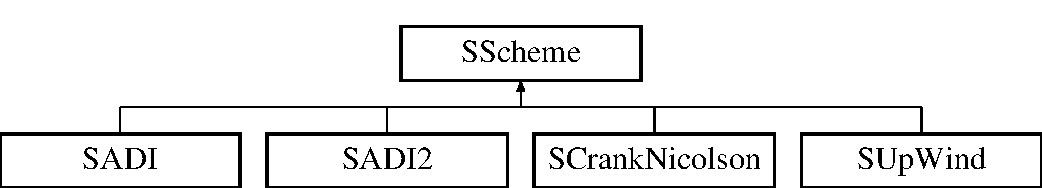
\includegraphics[height=2.000000cm]{class_s_scheme}
\end{center}
\end{figure}
\subsection*{Metody publiczne}
\begin{DoxyCompactItemize}
\item 
\hyperlink{class_s_scheme_a007f3a5b981419391f6a57222f7d7da6}{S\+Scheme} ()
\begin{DoxyCompactList}\small\item\em Konstruktor. \end{DoxyCompactList}\item 
virtual void \hyperlink{class_s_scheme_a1607f2363ea074bde9ad9c585b5a4019}{Compute\+Concentration} (map$<$ int, \hyperlink{class_point}{Point} $>$ \&Point\+Map)
\begin{DoxyCompactList}\small\item\em Oblicza koncentracje. \end{DoxyCompactList}\item 
void \hyperlink{class_s_scheme_a9f9da388c80058c59123ea58e28f6408}{Set\+Factors} (map$<$ int, \hyperlink{class_point}{Point} $>$ \&Point\+Map)
\begin{DoxyCompactList}\small\item\em Ustawia czynniki w rownaniu transportu dla calej siatki. \end{DoxyCompactList}\item 
virtual void \hyperlink{class_s_scheme_ae1e554b35ec2d8a902f6fdb30d95ab20}{Get\+Factors} (\hyperlink{class_point}{Point} $\ast$p, const double \&C\+Ax, const double \&C\+Ay, const double \&C\+Dx, const double \&C\+Dxy, const double \&C\+Dy, const vector$<$ int $>$ \&flag)
\begin{DoxyCompactList}\small\item\em Odpowiedzialna za wyznaczenie czynnikow w row transportu dla danego pkt. \end{DoxyCompactList}\item 
long double \hyperlink{class_s_scheme_a1b66164d72e54d4b85322fa68f307c30}{Jakobi} (\hyperlink{class_point}{Point} $\ast$p, map$<$ int, \hyperlink{class_point}{Point} $>$ \&Point\+Map, double fij, double a, double b, double c, double d, double e, double f, double g, double h, double i)
\begin{DoxyCompactList}\small\item\em metoda iteracyjna Jakobiego \end{DoxyCompactList}\item 
long double \hyperlink{class_s_scheme_a78c4706ab3f69423302451983ad44022}{Jakobi} (map$<$ int, \hyperlink{class_point}{Point} $>$ \&Point\+Map, map$<$ int, long double $>$ \&f, vector$<$ string $>$ \&a)
\item 
long double \hyperlink{class_s_scheme_a0dd0343c9bcb4b35849403d8a76f9d18}{Gauss\+\_\+\+Seidel} (\hyperlink{class_point}{Point} $\ast$p, map$<$ int, \hyperlink{class_point}{Point} $>$ \&Point\+Map, double fij, double a, double b, double c, double d, double e, double f, double g, double h, double i)
\begin{DoxyCompactList}\small\item\em metoda iteracyjna Gaussa Seidela \end{DoxyCompactList}\item 
long double \hyperlink{class_s_scheme_a48ee384f6206a5c55931a8e3361f7d57}{Gauss\+\_\+\+Seidel} (map$<$ int, \hyperlink{class_point}{Point} $>$ \&Point\+Map, map$<$ int, long double $>$ \&f, vector$<$ string $>$ \&a)
\item 
long double \hyperlink{class_s_scheme_a48fa493450e8c55967bdaa78e9e1bd7c}{S\+O\+R} (\hyperlink{class_point}{Point} $\ast$p, map$<$ int, \hyperlink{class_point}{Point} $>$ \&Point\+Map, double fij, double a, double b, double c, double d, double e, double f, double g, double h, double i, long double omega)
\begin{DoxyCompactList}\small\item\em metoda iteracyjna S\+O\+R \end{DoxyCompactList}\item 
long double \hyperlink{class_s_scheme_a4bf15feac00aed3dd724fbf4921a4144}{S\+O\+R} (map$<$ int, \hyperlink{class_point}{Point} $>$ \&Point\+Map, map$<$ int, long double $>$ \&f, vector$<$ string $>$ \&a, long double omega=1.\+0)
\item 
void \hyperlink{class_s_scheme_a2032e9d35d0931c17d8f96170d5d843a}{set\+\_\+sym\+\_\+step} (int step)
\item 
int \hyperlink{class_s_scheme_acadf8feab53234c5923990af908c2733}{get\+\_\+sym\+\_\+step} () const 
\item 
void \hyperlink{class_s_scheme_a99fefa3de0fa0859be662faa9e21a01b}{set\+\_\+omega} (long double omega)
\item 
long double \hyperlink{class_s_scheme_a69a8b9ea4d5c04b5def66db3d64c4c22}{get\+\_\+omega} () const 
\item 
void \hyperlink{class_s_scheme_a3749de0c92f9a4a50c10ded4d7713344}{set\+\_\+method} (string method)
\item 
string \hyperlink{class_s_scheme_a8c73b695beb2beb76079444aa92f7922}{get\+\_\+method} () const 
\item 
float \hyperlink{class_s_scheme_ab5e7404ff79c4c13d12f64e69b284027}{Find\+Best\+Omega} (map$<$ int, \hyperlink{class_point}{Point} $>$ \&Point\+Map, map$<$ int, long double $>$ \&f)
\item 
void \hyperlink{class_s_scheme_a04180646227c260880ddc35ee0b563e7}{Read\+Method} (string scheme)
\end{DoxyCompactItemize}
\subsection*{Atrybuty publiczne}
\begin{DoxyCompactItemize}
\item 
vector$<$ int $>$ \hyperlink{class_s_scheme_a875c9280df6dcdbc3a41ef1c148202da}{\+\_\+i}
\item 
map$<$ int, double $>$ \hyperlink{class_s_scheme_a7d998bc77fe043ec3dfba082bf7c570a}{\+\_\+w}
\item 
int \hyperlink{class_s_scheme_a6c8e7253815c7ac85996ee8fba438f53}{powrot}
\end{DoxyCompactItemize}


\subsection{Opis szczegółowy}
Klasa podstawowa Schematow. 

Zawiera metody potrzebane do rozwiazania rownania transportu w zaleznosci od wybranego schematu numrycznego uzywna sa metody z tej lub jednej z klas pochodnych. 

Definicja w linii 40 pliku scheme.\+h.



\subsection{Dokumentacja konstruktora i destruktora}
\hypertarget{class_s_scheme_a007f3a5b981419391f6a57222f7d7da6}{}\index{S\+Scheme@{S\+Scheme}!S\+Scheme@{S\+Scheme}}
\index{S\+Scheme@{S\+Scheme}!S\+Scheme@{S\+Scheme}}
\subsubsection[{S\+Scheme}]{\setlength{\rightskip}{0pt plus 5cm}S\+Scheme\+::\+S\+Scheme (
\begin{DoxyParamCaption}
{}
\end{DoxyParamCaption}
)\hspace{0.3cm}{\ttfamily [inline]}}\label{class_s_scheme_a007f3a5b981419391f6a57222f7d7da6}


Konstruktor. 

Tworzy schemat do rozwiazywania rownania transportu. 

Definicja w linii 47 pliku scheme.\+h.



\subsection{Dokumentacja funkcji składowych}
\hypertarget{class_s_scheme_a1607f2363ea074bde9ad9c585b5a4019}{}\index{S\+Scheme@{S\+Scheme}!Compute\+Concentration@{Compute\+Concentration}}
\index{Compute\+Concentration@{Compute\+Concentration}!S\+Scheme@{S\+Scheme}}
\subsubsection[{Compute\+Concentration}]{\setlength{\rightskip}{0pt plus 5cm}void S\+Scheme\+::\+Compute\+Concentration (
\begin{DoxyParamCaption}
\item[{map$<$ int, {\bf Point} $>$ \&}]{Point\+Map}
\end{DoxyParamCaption}
)\hspace{0.3cm}{\ttfamily [virtual]}}\label{class_s_scheme_a1607f2363ea074bde9ad9c585b5a4019}


Oblicza koncentracje. 

Oblicza koncentracje w daneym kroku uzywajac odpwoiedniej metody w zaeleznosci od wybranego schamtu do rozwiazywanie row transportu 
\begin{DoxyParams}{Parametry}
{\em Point\+Map} & -\/ mapa punktow \\
\hline
\end{DoxyParams}


Reimplementowana w \hyperlink{class_s_a_d_i2_a41903e3b443ba68fe68cbad73fe44970}{S\+A\+D\+I2}, \hyperlink{class_s_a_d_i_aed849c2b3b1a1c5b346edcfb69460457}{S\+A\+D\+I}, \hyperlink{class_s_up_wind_a500de829a9c8da4b43cb411014ff3b35}{S\+Up\+Wind} i \hyperlink{class_s_crank_nicolson_abe37e0a2d5078a17420b3e9d815fc85f}{S\+Crank\+Nicolson}.



Definicja w linii 24 pliku scheme.\+cpp.

\hypertarget{class_s_scheme_ab5e7404ff79c4c13d12f64e69b284027}{}\index{S\+Scheme@{S\+Scheme}!Find\+Best\+Omega@{Find\+Best\+Omega}}
\index{Find\+Best\+Omega@{Find\+Best\+Omega}!S\+Scheme@{S\+Scheme}}
\subsubsection[{Find\+Best\+Omega}]{\setlength{\rightskip}{0pt plus 5cm}float S\+Scheme\+::\+Find\+Best\+Omega (
\begin{DoxyParamCaption}
\item[{map$<$ int, {\bf Point} $>$ \&}]{Point\+Map, }
\item[{map$<$ int, long double $>$ \&}]{f}
\end{DoxyParamCaption}
)}\label{class_s_scheme_ab5e7404ff79c4c13d12f64e69b284027}


Definicja w linii 233 pliku scheme.\+cpp.

\hypertarget{class_s_scheme_a0dd0343c9bcb4b35849403d8a76f9d18}{}\index{S\+Scheme@{S\+Scheme}!Gauss\+\_\+\+Seidel@{Gauss\+\_\+\+Seidel}}
\index{Gauss\+\_\+\+Seidel@{Gauss\+\_\+\+Seidel}!S\+Scheme@{S\+Scheme}}
\subsubsection[{Gauss\+\_\+\+Seidel}]{\setlength{\rightskip}{0pt plus 5cm}long double S\+Scheme\+::\+Gauss\+\_\+\+Seidel (
\begin{DoxyParamCaption}
\item[{{\bf Point} $\ast$}]{p, }
\item[{map$<$ int, {\bf Point} $>$ \&}]{Point\+Map, }
\item[{double}]{fij, }
\item[{double}]{a, }
\item[{double}]{b, }
\item[{double}]{c, }
\item[{double}]{d, }
\item[{double}]{e, }
\item[{double}]{f, }
\item[{double}]{g, }
\item[{double}]{h, }
\item[{double}]{i}
\end{DoxyParamCaption}
)}\label{class_s_scheme_a0dd0343c9bcb4b35849403d8a76f9d18}


metoda iteracyjna Gaussa Seidela 

Wyznacza koncentracje w danym punkcie rozwiazywanego ukladu rownan, uzywajac formuly iteracyjne Gaussa Seidela do rozwiazywanai ukladow rownan linowych


\begin{DoxyParams}{Parametry}
{\em $\ast$p} & -\/ wskaznik do pktu dla ktorego obliczana jest wartosc koncentracji \\
\hline
{\em Point\+Map} & -\/ referencja do mapy punktow siatki \\
\hline
{\em fij} & -\/ wartosc wyrazu wolnego odpowiedniego dla danego pkt \\
\hline
{\em a,b,c,d,e,f,g,h,i} & -\/ wspolczynniki ukl rownnan odpowiednie dla danego pkt \\
\hline
\end{DoxyParams}
\begin{DoxyReturn}{Zwraca}
koncentracje dla danego pkt 
\end{DoxyReturn}


Definicja w linii 143 pliku scheme.\+cpp.

\hypertarget{class_s_scheme_a48ee384f6206a5c55931a8e3361f7d57}{}\index{S\+Scheme@{S\+Scheme}!Gauss\+\_\+\+Seidel@{Gauss\+\_\+\+Seidel}}
\index{Gauss\+\_\+\+Seidel@{Gauss\+\_\+\+Seidel}!S\+Scheme@{S\+Scheme}}
\subsubsection[{Gauss\+\_\+\+Seidel}]{\setlength{\rightskip}{0pt plus 5cm}long double S\+Scheme\+::\+Gauss\+\_\+\+Seidel (
\begin{DoxyParamCaption}
\item[{map$<$ int, {\bf Point} $>$ \&}]{Point\+Map, }
\item[{map$<$ int, long double $>$ \&}]{f, }
\item[{vector$<$ string $>$ \&}]{a}
\end{DoxyParamCaption}
)}\label{class_s_scheme_a48ee384f6206a5c55931a8e3361f7d57}


Definicja w linii 160 pliku scheme.\+cpp.

\hypertarget{class_s_scheme_a8c73b695beb2beb76079444aa92f7922}{}\index{S\+Scheme@{S\+Scheme}!get\+\_\+method@{get\+\_\+method}}
\index{get\+\_\+method@{get\+\_\+method}!S\+Scheme@{S\+Scheme}}
\subsubsection[{get\+\_\+method}]{\setlength{\rightskip}{0pt plus 5cm}string S\+Scheme\+::get\+\_\+method (
\begin{DoxyParamCaption}
{}
\end{DoxyParamCaption}
) const\hspace{0.3cm}{\ttfamily [inline]}}\label{class_s_scheme_a8c73b695beb2beb76079444aa92f7922}
zwraca wrtosc metody ktora ma byc uzyta do rozwiazywania ukladow rownan 

Definicja w linii 170 pliku scheme.\+h.

\hypertarget{class_s_scheme_a69a8b9ea4d5c04b5def66db3d64c4c22}{}\index{S\+Scheme@{S\+Scheme}!get\+\_\+omega@{get\+\_\+omega}}
\index{get\+\_\+omega@{get\+\_\+omega}!S\+Scheme@{S\+Scheme}}
\subsubsection[{get\+\_\+omega}]{\setlength{\rightskip}{0pt plus 5cm}long double S\+Scheme\+::get\+\_\+omega (
\begin{DoxyParamCaption}
{}
\end{DoxyParamCaption}
) const\hspace{0.3cm}{\ttfamily [inline]}}\label{class_s_scheme_a69a8b9ea4d5c04b5def66db3d64c4c22}
zwraca wrtosc rowna aktualnemu krokowi symulacji (potrzebny do S\+O\+Ra) 

Definicja w linii 164 pliku scheme.\+h.

\hypertarget{class_s_scheme_acadf8feab53234c5923990af908c2733}{}\index{S\+Scheme@{S\+Scheme}!get\+\_\+sym\+\_\+step@{get\+\_\+sym\+\_\+step}}
\index{get\+\_\+sym\+\_\+step@{get\+\_\+sym\+\_\+step}!S\+Scheme@{S\+Scheme}}
\subsubsection[{get\+\_\+sym\+\_\+step}]{\setlength{\rightskip}{0pt plus 5cm}int S\+Scheme\+::get\+\_\+sym\+\_\+step (
\begin{DoxyParamCaption}
{}
\end{DoxyParamCaption}
) const\hspace{0.3cm}{\ttfamily [inline]}}\label{class_s_scheme_acadf8feab53234c5923990af908c2733}
zwraca wrtosc rowna aktualnemu krokowi symulacji (potrzebny do S\+O\+Ra) 

Definicja w linii 158 pliku scheme.\+h.

\hypertarget{class_s_scheme_ae1e554b35ec2d8a902f6fdb30d95ab20}{}\index{S\+Scheme@{S\+Scheme}!Get\+Factors@{Get\+Factors}}
\index{Get\+Factors@{Get\+Factors}!S\+Scheme@{S\+Scheme}}
\subsubsection[{Get\+Factors}]{\setlength{\rightskip}{0pt plus 5cm}void S\+Scheme\+::\+Get\+Factors (
\begin{DoxyParamCaption}
\item[{{\bf Point} $\ast$}]{p, }
\item[{const double \&}]{C\+Ax, }
\item[{const double \&}]{C\+Ay, }
\item[{const double \&}]{C\+Dx, }
\item[{const double \&}]{C\+Dxy, }
\item[{const double \&}]{C\+Dy, }
\item[{const vector$<$ int $>$ \&}]{flag}
\end{DoxyParamCaption}
)\hspace{0.3cm}{\ttfamily [virtual]}}\label{class_s_scheme_ae1e554b35ec2d8a902f6fdb30d95ab20}


Odpowiedzialna za wyznaczenie czynnikow w row transportu dla danego pkt. 

Odpowiedzilan za wyznaczenie czynnikow (a, b, c, d, e, f, g, h, i) i (fa, fb, fc, fd, fe, ff, fg, fh, fi) w rowenanie transportu dal zadanego pkt w ktorym obliczana jest koncentracja w zaleznosci od schematu jaki wykorzystywany jest do rozwiazania rownania 
\begin{DoxyParams}{Parametry}
{\em $\ast$p} & -\/ pkt dla ktorego wyznaczane sa czynniki \\
\hline
{\em C\+Ax} & -\/ adwekcyjna liczba Couranta w kieruynku x \\
\hline
{\em C\+Ay} & -\/ adwekcyjna liczba Couranta w kieruynku y \\
\hline
{\em C\+Dx} & -\/ dyfuzyjna liczba Couranta w kieruynku x \\
\hline
{\em C\+Dxy} & -\/ dyfuzyjna liczba Couranta w kieruynku xy \\
\hline
{\em C\+Dy} & -\/ dyfuzyjna liczba Couranta w kieruynku y \\
\hline
\end{DoxyParams}


Reimplementowana w \hyperlink{class_s_a_d_i2_afac90c203840a07b31f73418af815063}{S\+A\+D\+I2}, \hyperlink{class_s_a_d_i_aec6b8007d89c0c72648b4cad7aba1274}{S\+A\+D\+I}, \hyperlink{class_s_up_wind_a64e2e7d8ce37fd489c375fdd9a99c105}{S\+Up\+Wind} i \hyperlink{class_s_crank_nicolson_a1fd8e8aee2c7fb9f61e6c4b02b74e1b3}{S\+Crank\+Nicolson}.



Definicja w linii 98 pliku scheme.\+cpp.

\hypertarget{class_s_scheme_a1b66164d72e54d4b85322fa68f307c30}{}\index{S\+Scheme@{S\+Scheme}!Jakobi@{Jakobi}}
\index{Jakobi@{Jakobi}!S\+Scheme@{S\+Scheme}}
\subsubsection[{Jakobi}]{\setlength{\rightskip}{0pt plus 5cm}long double S\+Scheme\+::\+Jakobi (
\begin{DoxyParamCaption}
\item[{{\bf Point} $\ast$}]{p, }
\item[{map$<$ int, {\bf Point} $>$ \&}]{Point\+Map, }
\item[{double}]{fij, }
\item[{double}]{a, }
\item[{double}]{b, }
\item[{double}]{c, }
\item[{double}]{d, }
\item[{double}]{e, }
\item[{double}]{f, }
\item[{double}]{g, }
\item[{double}]{h, }
\item[{double}]{i}
\end{DoxyParamCaption}
)}\label{class_s_scheme_a1b66164d72e54d4b85322fa68f307c30}


metoda iteracyjna Jakobiego 

Wyznacza koncentracje w danym punkcie rozwiazywanego ukladu rownan, uzywajac formuly iteracyjne Jakobiego do rozwiazywanai ukladow rownan linowych


\begin{DoxyParams}{Parametry}
{\em $\ast$p} & -\/ wskaznik do pktu dla ktorego obliczana jest wartosc koncentracji \\
\hline
{\em Point\+Map} & -\/ referencja do mapy punktow siatki \\
\hline
{\em fij} & -\/ wartosc wyrazu wolnego odpowiedniego dla danego pkt \\
\hline
{\em a,b,c,d,e,f,g,h,i} & -\/ wspolczynniki ukl rownnan odpowiednie dla danego pkt \\
\hline
\end{DoxyParams}
\begin{DoxyReturn}{Zwraca}
koncentracje dla danego pkt 
\end{DoxyReturn}


Definicja w linii 102 pliku scheme.\+cpp.

\hypertarget{class_s_scheme_a78c4706ab3f69423302451983ad44022}{}\index{S\+Scheme@{S\+Scheme}!Jakobi@{Jakobi}}
\index{Jakobi@{Jakobi}!S\+Scheme@{S\+Scheme}}
\subsubsection[{Jakobi}]{\setlength{\rightskip}{0pt plus 5cm}long double S\+Scheme\+::\+Jakobi (
\begin{DoxyParamCaption}
\item[{map$<$ int, {\bf Point} $>$ \&}]{Point\+Map, }
\item[{map$<$ int, long double $>$ \&}]{f, }
\item[{vector$<$ string $>$ \&}]{a}
\end{DoxyParamCaption}
)}\label{class_s_scheme_a78c4706ab3f69423302451983ad44022}


Definicja w linii 117 pliku scheme.\+cpp.

\hypertarget{class_s_scheme_a04180646227c260880ddc35ee0b563e7}{}\index{S\+Scheme@{S\+Scheme}!Read\+Method@{Read\+Method}}
\index{Read\+Method@{Read\+Method}!S\+Scheme@{S\+Scheme}}
\subsubsection[{Read\+Method}]{\setlength{\rightskip}{0pt plus 5cm}void S\+Scheme\+::\+Read\+Method (
\begin{DoxyParamCaption}
\item[{string}]{scheme}
\end{DoxyParamCaption}
)}\label{class_s_scheme_a04180646227c260880ddc35ee0b563e7}


Definicja w linii 239 pliku scheme.\+cpp.

\hypertarget{class_s_scheme_a3749de0c92f9a4a50c10ded4d7713344}{}\index{S\+Scheme@{S\+Scheme}!set\+\_\+method@{set\+\_\+method}}
\index{set\+\_\+method@{set\+\_\+method}!S\+Scheme@{S\+Scheme}}
\subsubsection[{set\+\_\+method}]{\setlength{\rightskip}{0pt plus 5cm}void S\+Scheme\+::set\+\_\+method (
\begin{DoxyParamCaption}
\item[{string}]{method}
\end{DoxyParamCaption}
)\hspace{0.3cm}{\ttfamily [inline]}}\label{class_s_scheme_a3749de0c92f9a4a50c10ded4d7713344}
ustawia metode ktora ma byc uzyta do rozwiazywania ukladow rownan 

Definicja w linii 167 pliku scheme.\+h.

\hypertarget{class_s_scheme_a99fefa3de0fa0859be662faa9e21a01b}{}\index{S\+Scheme@{S\+Scheme}!set\+\_\+omega@{set\+\_\+omega}}
\index{set\+\_\+omega@{set\+\_\+omega}!S\+Scheme@{S\+Scheme}}
\subsubsection[{set\+\_\+omega}]{\setlength{\rightskip}{0pt plus 5cm}void S\+Scheme\+::set\+\_\+omega (
\begin{DoxyParamCaption}
\item[{long double}]{omega}
\end{DoxyParamCaption}
)\hspace{0.3cm}{\ttfamily [inline]}}\label{class_s_scheme_a99fefa3de0fa0859be662faa9e21a01b}
ustawia wartosc rowna aktualnemu krokowi symulacji (potrzebny do S\+O\+Ra) 

Definicja w linii 161 pliku scheme.\+h.

\hypertarget{class_s_scheme_a2032e9d35d0931c17d8f96170d5d843a}{}\index{S\+Scheme@{S\+Scheme}!set\+\_\+sym\+\_\+step@{set\+\_\+sym\+\_\+step}}
\index{set\+\_\+sym\+\_\+step@{set\+\_\+sym\+\_\+step}!S\+Scheme@{S\+Scheme}}
\subsubsection[{set\+\_\+sym\+\_\+step}]{\setlength{\rightskip}{0pt plus 5cm}void S\+Scheme\+::set\+\_\+sym\+\_\+step (
\begin{DoxyParamCaption}
\item[{int}]{step}
\end{DoxyParamCaption}
)\hspace{0.3cm}{\ttfamily [inline]}}\label{class_s_scheme_a2032e9d35d0931c17d8f96170d5d843a}
ustawia wartosc rowna aktualnemu krokowi symulacji (potrzebny do S\+O\+Ra) 

Definicja w linii 155 pliku scheme.\+h.

\hypertarget{class_s_scheme_a9f9da388c80058c59123ea58e28f6408}{}\index{S\+Scheme@{S\+Scheme}!Set\+Factors@{Set\+Factors}}
\index{Set\+Factors@{Set\+Factors}!S\+Scheme@{S\+Scheme}}
\subsubsection[{Set\+Factors}]{\setlength{\rightskip}{0pt plus 5cm}void S\+Scheme\+::\+Set\+Factors (
\begin{DoxyParamCaption}
\item[{map$<$ int, {\bf Point} $>$ \&}]{Point\+Map}
\end{DoxyParamCaption}
)}\label{class_s_scheme_a9f9da388c80058c59123ea58e28f6408}


Ustawia czynniki w rownaniu transportu dla calej siatki. 

Ustawia czynniki (a, b, c, d, e, f, g, h, i) i (fa, fb, fc, fd, fe, ff, fg, fh, fi) w rownaniu transportu dla wszytskich pktow

\[ a~c_{i,j}^{n+1} + b~c_{i+1,j}^{n+1} + c~c_{i-1,j}^{n+1} + d~c_{i,j+1}^{n+1} + e~c_{i,j-1}^{n+1} + f~c_{i+1,j+1}^{n+1} + g~c_{i+1,j-1}^{n+1} + h~c_{i-1,j+1}^{n+1} + i~c_{i-1,j-1}^{n+1} \] \[ = fa~c_{i,j}^{n} + fb~c_{i+1,j}^{n} + fc~c_{i-1,j}^{n} + fd~c_{i,j+1}^{n} + fe~c_{i,j-1}^{n} + ff~c_{i+1,j+1}^{n} + fg~c_{i+1,j-1}^{n} + fh~c_{i-1,j+1}^{n} + fi~c_{i-1,j-1}^{n} \]


\begin{DoxyParams}{Parametry}
{\em Point\+Map} & -\/ mapa punktow \\
\hline
\end{DoxyParams}


Definicja w linii 27 pliku scheme.\+cpp.

\hypertarget{class_s_scheme_a48fa493450e8c55967bdaa78e9e1bd7c}{}\index{S\+Scheme@{S\+Scheme}!S\+O\+R@{S\+O\+R}}
\index{S\+O\+R@{S\+O\+R}!S\+Scheme@{S\+Scheme}}
\subsubsection[{S\+O\+R}]{\setlength{\rightskip}{0pt plus 5cm}long double S\+Scheme\+::\+S\+O\+R (
\begin{DoxyParamCaption}
\item[{{\bf Point} $\ast$}]{p, }
\item[{map$<$ int, {\bf Point} $>$ \&}]{Point\+Map, }
\item[{double}]{fij, }
\item[{double}]{a, }
\item[{double}]{b, }
\item[{double}]{c, }
\item[{double}]{d, }
\item[{double}]{e, }
\item[{double}]{f, }
\item[{double}]{g, }
\item[{double}]{h, }
\item[{double}]{i, }
\item[{long double}]{omega}
\end{DoxyParamCaption}
)}\label{class_s_scheme_a48fa493450e8c55967bdaa78e9e1bd7c}


metoda iteracyjna S\+O\+R 

Wyznacza koncentracje w danym punkcie rozwiazywanego ukladu rownan, uzywajac formuly iteracyjne S\+O\+R (Saccessive Over Relaksation) do rozwiazywanai ukladow rownan linowych


\begin{DoxyParams}{Parametry}
{\em $\ast$p} & -\/ wskaznik do pktu dla ktorego obliczana jest wartosc koncentracji \\
\hline
{\em Point\+Map} & -\/ referencja do mapy punktow siatki \\
\hline
{\em fij} & -\/ wartosc wyrazu wolnego odpowiedniego dla danego pkt \\
\hline
{\em a,b,c,d,e,f,g,h,i} & -\/ wspolczynniki ukl rownnan odpowiednie dla danego pkt \\
\hline
{\em omega} & -\/ parametr relaksacji \\
\hline
\end{DoxyParams}
\begin{DoxyReturn}{Zwraca}
koncentracje dla danego pkt 
\end{DoxyReturn}


Definicja w linii 185 pliku scheme.\+cpp.

\hypertarget{class_s_scheme_a4bf15feac00aed3dd724fbf4921a4144}{}\index{S\+Scheme@{S\+Scheme}!S\+O\+R@{S\+O\+R}}
\index{S\+O\+R@{S\+O\+R}!S\+Scheme@{S\+Scheme}}
\subsubsection[{S\+O\+R}]{\setlength{\rightskip}{0pt plus 5cm}long double S\+Scheme\+::\+S\+O\+R (
\begin{DoxyParamCaption}
\item[{map$<$ int, {\bf Point} $>$ \&}]{Point\+Map, }
\item[{map$<$ int, long double $>$ \&}]{f, }
\item[{vector$<$ string $>$ \&}]{a, }
\item[{long double}]{omega = {\ttfamily 1.0}}
\end{DoxyParamCaption}
)}\label{class_s_scheme_a4bf15feac00aed3dd724fbf4921a4144}


Definicja w linii 208 pliku scheme.\+cpp.



\subsection{Dokumentacja atrybutów składowych}
\hypertarget{class_s_scheme_a875c9280df6dcdbc3a41ef1c148202da}{}\index{S\+Scheme@{S\+Scheme}!\+\_\+i@{\+\_\+i}}
\index{\+\_\+i@{\+\_\+i}!S\+Scheme@{S\+Scheme}}
\subsubsection[{\+\_\+i}]{\setlength{\rightskip}{0pt plus 5cm}vector$<$int$>$ S\+Scheme\+::\+\_\+i}\label{class_s_scheme_a875c9280df6dcdbc3a41ef1c148202da}


Definicja w linii 177 pliku scheme.\+h.

\hypertarget{class_s_scheme_a7d998bc77fe043ec3dfba082bf7c570a}{}\index{S\+Scheme@{S\+Scheme}!\+\_\+w@{\+\_\+w}}
\index{\+\_\+w@{\+\_\+w}!S\+Scheme@{S\+Scheme}}
\subsubsection[{\+\_\+w}]{\setlength{\rightskip}{0pt plus 5cm}map$<$int,double$>$ S\+Scheme\+::\+\_\+w}\label{class_s_scheme_a7d998bc77fe043ec3dfba082bf7c570a}


Definicja w linii 178 pliku scheme.\+h.

\hypertarget{class_s_scheme_a6c8e7253815c7ac85996ee8fba438f53}{}\index{S\+Scheme@{S\+Scheme}!powrot@{powrot}}
\index{powrot@{powrot}!S\+Scheme@{S\+Scheme}}
\subsubsection[{powrot}]{\setlength{\rightskip}{0pt plus 5cm}int S\+Scheme\+::powrot}\label{class_s_scheme_a6c8e7253815c7ac85996ee8fba438f53}


Definicja w linii 179 pliku scheme.\+h.



Dokumentacja dla tej klasy została wygenerowana z plików\+:\begin{DoxyCompactItemize}
\item 
\hyperlink{scheme_8h}{scheme.\+h}\item 
\hyperlink{scheme_8cpp}{scheme.\+cpp}\item 
\hyperlink{scheme__new__bez_q_8cpp}{scheme\+\_\+new\+\_\+bez\+Q.\+cpp}\item 
\hyperlink{scheme__new__z_q_8cpp}{scheme\+\_\+new\+\_\+z\+Q.\+cpp}\item 
\hyperlink{scheme__przed__zmina__09092015_8cpp}{scheme\+\_\+przed\+\_\+zmina\+\_\+09092015.\+cpp}\end{DoxyCompactItemize}

\hypertarget{class_s_up_wind}{}\section{Dokumentacja klasy S\+Up\+Wind}
\label{class_s_up_wind}\index{S\+Up\+Wind@{S\+Up\+Wind}}


Schemat Pod Prad (Up\+Wind).  




{\ttfamily \#include $<$scheme.\+h$>$}

Diagram dziedziczenia dla S\+Up\+Wind\begin{figure}[H]
\begin{center}
\leavevmode
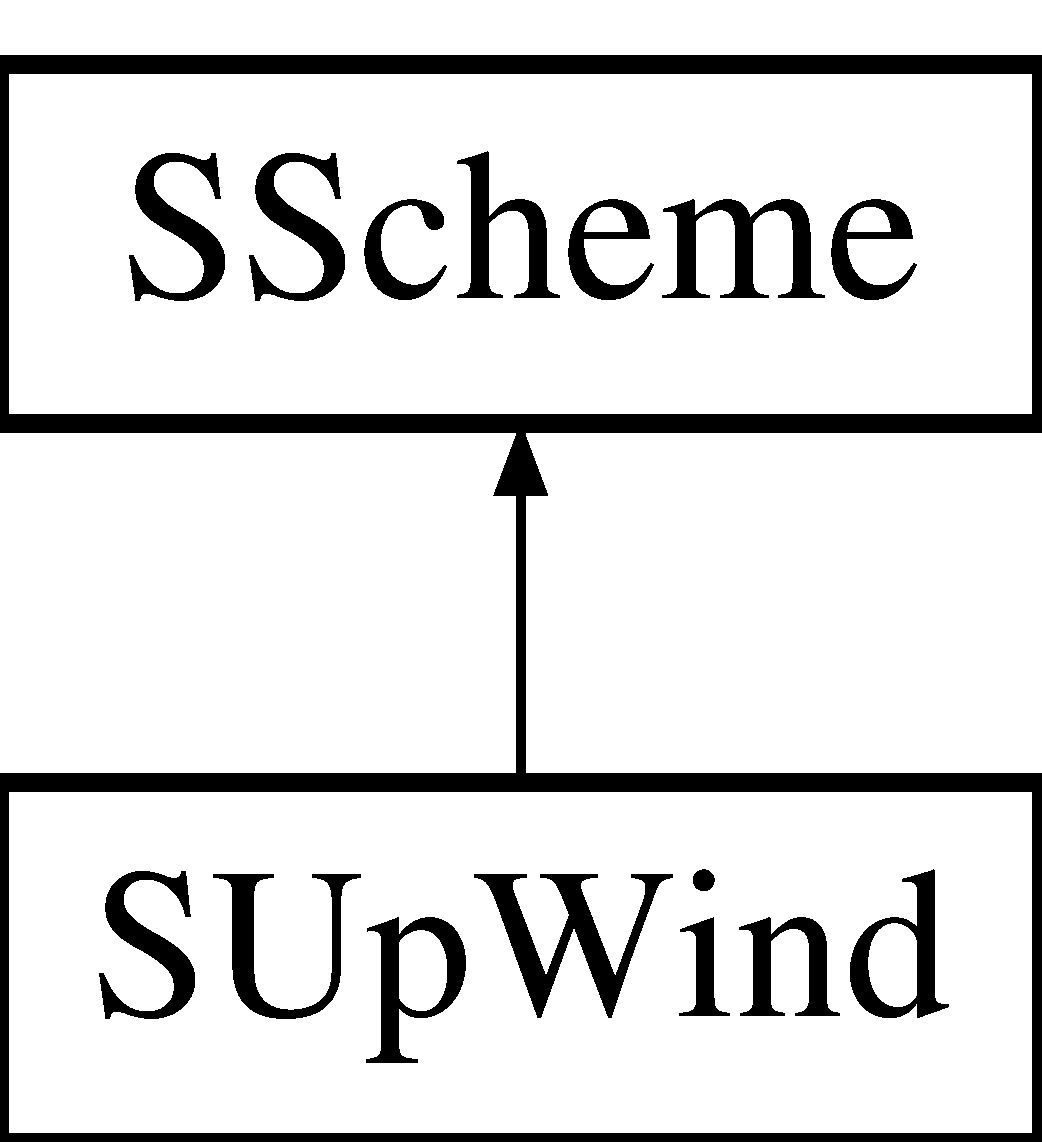
\includegraphics[height=2.000000cm]{class_s_up_wind}
\end{center}
\end{figure}
\subsection*{Metody publiczne}
\begin{DoxyCompactItemize}
\item 
\hyperlink{class_s_up_wind_a92e3d5f059c9f8ae6e1ee5e3d547f144}{S\+Up\+Wind} ()
\begin{DoxyCompactList}\small\item\em Konstruktor. \end{DoxyCompactList}\item 
void \hyperlink{class_s_up_wind_a500de829a9c8da4b43cb411014ff3b35}{Compute\+Concentration} (map$<$ int, \hyperlink{class_point}{Point} $>$ \&Point\+Map)
\begin{DoxyCompactList}\small\item\em Oblicza koncentracje uzywajac schamatu Up\+Wind. \end{DoxyCompactList}\item 
void \hyperlink{class_s_up_wind_a64e2e7d8ce37fd489c375fdd9a99c105}{Get\+Factors} (\hyperlink{class_point}{Point} $\ast$p, const double \&C\+Ax, const double \&C\+Ay, const double \&C\+Dx, const double \&C\+Dxy, const double \&C\+Dy, const vector$<$ int $>$ \&flag)
\end{DoxyCompactItemize}
\subsection*{Dodatkowe Dziedziczone Składowe}


\subsection{Opis szczegółowy}
Schemat Pod Prad (Up\+Wind). 

Zawiera metody potrzebane do rozwiazania rownania transportu metoda Pod Prad. 

Definicja w linii 240 pliku scheme.\+h.



\subsection{Dokumentacja konstruktora i destruktora}
\hypertarget{class_s_up_wind_a92e3d5f059c9f8ae6e1ee5e3d547f144}{}\index{S\+Up\+Wind@{S\+Up\+Wind}!S\+Up\+Wind@{S\+Up\+Wind}}
\index{S\+Up\+Wind@{S\+Up\+Wind}!S\+Up\+Wind@{S\+Up\+Wind}}
\subsubsection[{S\+Up\+Wind}]{\setlength{\rightskip}{0pt plus 5cm}S\+Up\+Wind\+::\+S\+Up\+Wind (
\begin{DoxyParamCaption}
{}
\end{DoxyParamCaption}
)\hspace{0.3cm}{\ttfamily [inline]}}\label{class_s_up_wind_a92e3d5f059c9f8ae6e1ee5e3d547f144}


Konstruktor. 

Tworzy schemat do rozwiazywania rownania transporu metoda Up\+Wind 

Definicja w linii 248 pliku scheme.\+h.



\subsection{Dokumentacja funkcji składowych}
\hypertarget{class_s_up_wind_a500de829a9c8da4b43cb411014ff3b35}{}\index{S\+Up\+Wind@{S\+Up\+Wind}!Compute\+Concentration@{Compute\+Concentration}}
\index{Compute\+Concentration@{Compute\+Concentration}!S\+Up\+Wind@{S\+Up\+Wind}}
\subsubsection[{Compute\+Concentration}]{\setlength{\rightskip}{0pt plus 5cm}void S\+Up\+Wind\+::\+Compute\+Concentration (
\begin{DoxyParamCaption}
\item[{map$<$ int, {\bf Point} $>$ \&}]{Point\+Map}
\end{DoxyParamCaption}
)\hspace{0.3cm}{\ttfamily [virtual]}}\label{class_s_up_wind_a500de829a9c8da4b43cb411014ff3b35}


Oblicza koncentracje uzywajac schamatu Up\+Wind. 

Oblicza koncentracje w daneym kroku uzywajac metody Up\+Wind 
\begin{DoxyParams}{Parametry}
{\em Point\+Map} & -\/ mapa punktow \\
\hline
\end{DoxyParams}
10.\+06.\+2015 -\/ dodajemy czlon zrodluwy

10.\+06.\+2015 -\/ dodajemy czlon zrodluwy 

Reimplementowana z \hyperlink{class_s_scheme_a1607f2363ea074bde9ad9c585b5a4019}{S\+Scheme}.



Definicja w linii 809 pliku scheme.\+cpp.

\hypertarget{class_s_up_wind_a64e2e7d8ce37fd489c375fdd9a99c105}{}\index{S\+Up\+Wind@{S\+Up\+Wind}!Get\+Factors@{Get\+Factors}}
\index{Get\+Factors@{Get\+Factors}!S\+Up\+Wind@{S\+Up\+Wind}}
\subsubsection[{Get\+Factors}]{\setlength{\rightskip}{0pt plus 5cm}void S\+Up\+Wind\+::\+Get\+Factors (
\begin{DoxyParamCaption}
\item[{{\bf Point} $\ast$}]{p, }
\item[{const double \&}]{C\+Ax, }
\item[{const double \&}]{C\+Ay, }
\item[{const double \&}]{C\+Dx, }
\item[{const double \&}]{C\+Dxy, }
\item[{const double \&}]{C\+Dy, }
\item[{const vector$<$ int $>$ \&}]{flag}
\end{DoxyParamCaption}
)\hspace{0.3cm}{\ttfamily [virtual]}}\label{class_s_up_wind_a64e2e7d8ce37fd489c375fdd9a99c105}
Odpowiedzilan za wyznaczenie czynnikow (a, b, c, d, e, f, g, h, i) i (fa, fb, fc, fd, fe, ff, fg, fh, fi) w rowenanie transportu dal zadanego pkt w ktorym obliczana jest koncentracja dla schemtau Up\+Wind


\begin{DoxyParams}{Parametry}
{\em $\ast$p} & -\/ pkt dla ktorego wyznaczane sa czynniki \\
\hline
{\em C\+Ax} & -\/ adwekcyjna liczba Couranta w kieruynku x \\
\hline
{\em C\+Ay} & -\/ adwekcyjna liczba Couranta w kieruynku y \\
\hline
{\em C\+Dx} & -\/ dyfuzyjna liczba Couranta w kieruynku x \\
\hline
{\em C\+Dxy} & -\/ dyfuzyjna liczba Couranta w kieruynku xy \\
\hline
{\em C\+Dy} & -\/ dyfuzyjna liczba Couranta w kieruynku y \\
\hline
\end{DoxyParams}


Reimplementowana z \hyperlink{class_s_scheme_ae1e554b35ec2d8a902f6fdb30d95ab20}{S\+Scheme}.



Definicja w linii 863 pliku scheme.\+cpp.



Dokumentacja dla tej klasy została wygenerowana z plików\+:\begin{DoxyCompactItemize}
\item 
\hyperlink{scheme_8h}{scheme.\+h}\item 
\hyperlink{scheme_8cpp}{scheme.\+cpp}\item 
\hyperlink{scheme__new__bez_q_8cpp}{scheme\+\_\+new\+\_\+bez\+Q.\+cpp}\item 
\hyperlink{scheme__new__z_q_8cpp}{scheme\+\_\+new\+\_\+z\+Q.\+cpp}\item 
\hyperlink{scheme__przed__zmina__09092015_8cpp}{scheme\+\_\+przed\+\_\+zmina\+\_\+09092015.\+cpp}\end{DoxyCompactItemize}

\chapter{Dokumentacja plików}
\hypertarget{_c_make_c_compiler_id_8c}{}\section{Dokumentacja pliku build/\+C\+Make\+Files/3.0.2/\+Compiler\+Id\+C/\+C\+Make\+C\+Compiler\+Id.c}
\label{_c_make_c_compiler_id_8c}\index{build/\+C\+Make\+Files/3.\+0.\+2/\+Compiler\+Id\+C/\+C\+Make\+C\+Compiler\+Id.\+c@{build/\+C\+Make\+Files/3.\+0.\+2/\+Compiler\+Id\+C/\+C\+Make\+C\+Compiler\+Id.\+c}}
\subsection*{Definicje}
\begin{DoxyCompactItemize}
\item 
\#define \hyperlink{_c_make_c_compiler_id_8c_a81dee0709ded976b2e0319239f72d174}{C\+O\+M\+P\+I\+L\+E\+R\+\_\+\+I\+D}~\char`\"{}\char`\"{}
\item 
\#define \hyperlink{_c_make_c_compiler_id_8c_adbc5372f40838899018fadbc89bd588b}{P\+L\+A\+T\+F\+O\+R\+M\+\_\+\+I\+D}~\char`\"{}\char`\"{}
\item 
\#define \hyperlink{_c_make_c_compiler_id_8c_aba35d0d200deaeb06aee95ca297acb28}{A\+R\+C\+H\+I\+T\+E\+C\+T\+U\+R\+E\+\_\+\+I\+D}~\char`\"{}\char`\"{}
\item 
\#define \hyperlink{_c_make_c_compiler_id_8c_ad1280362da42492bbc11aa78cbf776ad}{D\+E\+C}(n)
\item 
\#define \hyperlink{_c_make_c_compiler_id_8c_a46d5d95daa1bef867bd0179594310ed5}{H\+E\+X}(n)
\end{DoxyCompactItemize}
\subsection*{Funkcje}
\begin{DoxyCompactItemize}
\item 
int \hyperlink{_c_make_c_compiler_id_8c_a0ddf1224851353fc92bfbff6f499fa97}{main} (int argc, char $\ast$argv\mbox{[}$\,$\mbox{]})
\end{DoxyCompactItemize}
\subsection*{Zmienne}
\begin{DoxyCompactItemize}
\item 
char const $\ast$ \hyperlink{_c_make_c_compiler_id_8c_a4b0efeb7a5d59313986b3a0390f050f6}{info\+\_\+compiler} = \char`\"{}I\+N\+F\+O\char`\"{} \char`\"{}\+:\char`\"{} \char`\"{}compiler\mbox{[}\char`\"{} C\+O\+M\+P\+I\+L\+E\+R\+\_\+\+I\+D \char`\"{}\mbox{]}\char`\"{}
\item 
char const $\ast$ \hyperlink{_c_make_c_compiler_id_8c_a2321403dee54ee23f0c2fa849c60f7d4}{info\+\_\+platform} = \char`\"{}I\+N\+F\+O\char`\"{} \char`\"{}\+:\char`\"{} \char`\"{}platform\mbox{[}\char`\"{} P\+L\+A\+T\+F\+O\+R\+M\+\_\+\+I\+D \char`\"{}\mbox{]}\char`\"{}
\item 
char const $\ast$ \hyperlink{_c_make_c_compiler_id_8c_a59647e99d304ed33b15cb284c27ed391}{info\+\_\+arch} = \char`\"{}I\+N\+F\+O\char`\"{} \char`\"{}\+:\char`\"{} \char`\"{}arch\mbox{[}\char`\"{} A\+R\+C\+H\+I\+T\+E\+C\+T\+U\+R\+E\+\_\+\+I\+D \char`\"{}\mbox{]}\char`\"{}
\end{DoxyCompactItemize}


\subsection{Dokumentacja definicji}
\hypertarget{_c_make_c_compiler_id_8c_aba35d0d200deaeb06aee95ca297acb28}{}\index{C\+Make\+C\+Compiler\+Id.\+c@{C\+Make\+C\+Compiler\+Id.\+c}!A\+R\+C\+H\+I\+T\+E\+C\+T\+U\+R\+E\+\_\+\+I\+D@{A\+R\+C\+H\+I\+T\+E\+C\+T\+U\+R\+E\+\_\+\+I\+D}}
\index{A\+R\+C\+H\+I\+T\+E\+C\+T\+U\+R\+E\+\_\+\+I\+D@{A\+R\+C\+H\+I\+T\+E\+C\+T\+U\+R\+E\+\_\+\+I\+D}!C\+Make\+C\+Compiler\+Id.\+c@{C\+Make\+C\+Compiler\+Id.\+c}}
\subsubsection[{A\+R\+C\+H\+I\+T\+E\+C\+T\+U\+R\+E\+\_\+\+I\+D}]{\setlength{\rightskip}{0pt plus 5cm}\#define A\+R\+C\+H\+I\+T\+E\+C\+T\+U\+R\+E\+\_\+\+I\+D~\char`\"{}\char`\"{}}\label{_c_make_c_compiler_id_8c_aba35d0d200deaeb06aee95ca297acb28}


Definicja w linii 348 pliku C\+Make\+C\+Compiler\+Id.\+c.

\hypertarget{_c_make_c_compiler_id_8c_a81dee0709ded976b2e0319239f72d174}{}\index{C\+Make\+C\+Compiler\+Id.\+c@{C\+Make\+C\+Compiler\+Id.\+c}!C\+O\+M\+P\+I\+L\+E\+R\+\_\+\+I\+D@{C\+O\+M\+P\+I\+L\+E\+R\+\_\+\+I\+D}}
\index{C\+O\+M\+P\+I\+L\+E\+R\+\_\+\+I\+D@{C\+O\+M\+P\+I\+L\+E\+R\+\_\+\+I\+D}!C\+Make\+C\+Compiler\+Id.\+c@{C\+Make\+C\+Compiler\+Id.\+c}}
\subsubsection[{C\+O\+M\+P\+I\+L\+E\+R\+\_\+\+I\+D}]{\setlength{\rightskip}{0pt plus 5cm}\#define C\+O\+M\+P\+I\+L\+E\+R\+\_\+\+I\+D~\char`\"{}\char`\"{}}\label{_c_make_c_compiler_id_8c_a81dee0709ded976b2e0319239f72d174}


Definicja w linii 221 pliku C\+Make\+C\+Compiler\+Id.\+c.

\hypertarget{_c_make_c_compiler_id_8c_ad1280362da42492bbc11aa78cbf776ad}{}\index{C\+Make\+C\+Compiler\+Id.\+c@{C\+Make\+C\+Compiler\+Id.\+c}!D\+E\+C@{D\+E\+C}}
\index{D\+E\+C@{D\+E\+C}!C\+Make\+C\+Compiler\+Id.\+c@{C\+Make\+C\+Compiler\+Id.\+c}}
\subsubsection[{D\+E\+C}]{\setlength{\rightskip}{0pt plus 5cm}\#define D\+E\+C(
\begin{DoxyParamCaption}
\item[{}]{n}
\end{DoxyParamCaption}
)}\label{_c_make_c_compiler_id_8c_ad1280362da42492bbc11aa78cbf776ad}
{\bfseries Wartość\+:}
\begin{DoxyCode}
(\textcolor{charliteral}{'0'} + (((n) / 10000000)%10)), \(\backslash\)
  (\textcolor{charliteral}{'0'} + (((n) / 1000000)%10)),  \(\backslash\)
  (\textcolor{charliteral}{'0'} + (((n) / 100000)%10)),   \(\backslash\)
  (\textcolor{charliteral}{'0'} + (((n) / 10000)%10)),    \(\backslash\)
  (\textcolor{charliteral}{'0'} + (((n) / 1000)%10)),     \(\backslash\)
  (\textcolor{charliteral}{'0'} + (((n) / 100)%10)),      \(\backslash\)
  (\textcolor{charliteral}{'0'} + (((n) / 10)%10)),       \(\backslash\)
  (\textcolor{charliteral}{'0'} +  ((n) % 10))
\end{DoxyCode}


Definicja w linii 352 pliku C\+Make\+C\+Compiler\+Id.\+c.

\hypertarget{_c_make_c_compiler_id_8c_a46d5d95daa1bef867bd0179594310ed5}{}\index{C\+Make\+C\+Compiler\+Id.\+c@{C\+Make\+C\+Compiler\+Id.\+c}!H\+E\+X@{H\+E\+X}}
\index{H\+E\+X@{H\+E\+X}!C\+Make\+C\+Compiler\+Id.\+c@{C\+Make\+C\+Compiler\+Id.\+c}}
\subsubsection[{H\+E\+X}]{\setlength{\rightskip}{0pt plus 5cm}\#define H\+E\+X(
\begin{DoxyParamCaption}
\item[{}]{n}
\end{DoxyParamCaption}
)}\label{_c_make_c_compiler_id_8c_a46d5d95daa1bef867bd0179594310ed5}
{\bfseries Wartość\+:}
\begin{DoxyCode}
(\textcolor{charliteral}{'0'} + ((n)>>28 & 0xF)), \(\backslash\)
  (\textcolor{charliteral}{'0'} + ((n)>>24 & 0xF)), \(\backslash\)
  (\textcolor{charliteral}{'0'} + ((n)>>20 & 0xF)), \(\backslash\)
  (\textcolor{charliteral}{'0'} + ((n)>>16 & 0xF)), \(\backslash\)
  (\textcolor{charliteral}{'0'} + ((n)>>12 & 0xF)), \(\backslash\)
  (\textcolor{charliteral}{'0'} + ((n)>>8  & 0xF)), \(\backslash\)
  (\textcolor{charliteral}{'0'} + ((n)>>4  & 0xF)), \(\backslash\)
  (\textcolor{charliteral}{'0'} + ((n)     & 0xF))
\end{DoxyCode}


Definicja w linii 363 pliku C\+Make\+C\+Compiler\+Id.\+c.

\hypertarget{_c_make_c_compiler_id_8c_adbc5372f40838899018fadbc89bd588b}{}\index{C\+Make\+C\+Compiler\+Id.\+c@{C\+Make\+C\+Compiler\+Id.\+c}!P\+L\+A\+T\+F\+O\+R\+M\+\_\+\+I\+D@{P\+L\+A\+T\+F\+O\+R\+M\+\_\+\+I\+D}}
\index{P\+L\+A\+T\+F\+O\+R\+M\+\_\+\+I\+D@{P\+L\+A\+T\+F\+O\+R\+M\+\_\+\+I\+D}!C\+Make\+C\+Compiler\+Id.\+c@{C\+Make\+C\+Compiler\+Id.\+c}}
\subsubsection[{P\+L\+A\+T\+F\+O\+R\+M\+\_\+\+I\+D}]{\setlength{\rightskip}{0pt plus 5cm}\#define P\+L\+A\+T\+F\+O\+R\+M\+\_\+\+I\+D~\char`\"{}\char`\"{}}\label{_c_make_c_compiler_id_8c_adbc5372f40838899018fadbc89bd588b}


Definicja w linii 315 pliku C\+Make\+C\+Compiler\+Id.\+c.



\subsection{Dokumentacja funkcji}
\hypertarget{_c_make_c_compiler_id_8c_a0ddf1224851353fc92bfbff6f499fa97}{}\index{C\+Make\+C\+Compiler\+Id.\+c@{C\+Make\+C\+Compiler\+Id.\+c}!main@{main}}
\index{main@{main}!C\+Make\+C\+Compiler\+Id.\+c@{C\+Make\+C\+Compiler\+Id.\+c}}
\subsubsection[{main}]{\setlength{\rightskip}{0pt plus 5cm}int main (
\begin{DoxyParamCaption}
\item[{int}]{argc, }
\item[{char $\ast$}]{argv\mbox{[}$\,$\mbox{]}}
\end{DoxyParamCaption}
)}\label{_c_make_c_compiler_id_8c_a0ddf1224851353fc92bfbff6f499fa97}


Definicja w linii 424 pliku C\+Make\+C\+Compiler\+Id.\+c.



\subsection{Dokumentacja zmiennych}
\hypertarget{_c_make_c_compiler_id_8c_a59647e99d304ed33b15cb284c27ed391}{}\index{C\+Make\+C\+Compiler\+Id.\+c@{C\+Make\+C\+Compiler\+Id.\+c}!info\+\_\+arch@{info\+\_\+arch}}
\index{info\+\_\+arch@{info\+\_\+arch}!C\+Make\+C\+Compiler\+Id.\+c@{C\+Make\+C\+Compiler\+Id.\+c}}
\subsubsection[{info\+\_\+arch}]{\setlength{\rightskip}{0pt plus 5cm}char const$\ast$ info\+\_\+arch = \char`\"{}I\+N\+F\+O\char`\"{} \char`\"{}\+:\char`\"{} \char`\"{}arch\mbox{[}\char`\"{} A\+R\+C\+H\+I\+T\+E\+C\+T\+U\+R\+E\+\_\+\+I\+D \char`\"{}\mbox{]}\char`\"{}}\label{_c_make_c_compiler_id_8c_a59647e99d304ed33b15cb284c27ed391}


Definicja w linii 414 pliku C\+Make\+C\+Compiler\+Id.\+c.

\hypertarget{_c_make_c_compiler_id_8c_a4b0efeb7a5d59313986b3a0390f050f6}{}\index{C\+Make\+C\+Compiler\+Id.\+c@{C\+Make\+C\+Compiler\+Id.\+c}!info\+\_\+compiler@{info\+\_\+compiler}}
\index{info\+\_\+compiler@{info\+\_\+compiler}!C\+Make\+C\+Compiler\+Id.\+c@{C\+Make\+C\+Compiler\+Id.\+c}}
\subsubsection[{info\+\_\+compiler}]{\setlength{\rightskip}{0pt plus 5cm}char const$\ast$ info\+\_\+compiler = \char`\"{}I\+N\+F\+O\char`\"{} \char`\"{}\+:\char`\"{} \char`\"{}compiler\mbox{[}\char`\"{} C\+O\+M\+P\+I\+L\+E\+R\+\_\+\+I\+D \char`\"{}\mbox{]}\char`\"{}}\label{_c_make_c_compiler_id_8c_a4b0efeb7a5d59313986b3a0390f050f6}


Definicja w linii 229 pliku C\+Make\+C\+Compiler\+Id.\+c.

\hypertarget{_c_make_c_compiler_id_8c_a2321403dee54ee23f0c2fa849c60f7d4}{}\index{C\+Make\+C\+Compiler\+Id.\+c@{C\+Make\+C\+Compiler\+Id.\+c}!info\+\_\+platform@{info\+\_\+platform}}
\index{info\+\_\+platform@{info\+\_\+platform}!C\+Make\+C\+Compiler\+Id.\+c@{C\+Make\+C\+Compiler\+Id.\+c}}
\subsubsection[{info\+\_\+platform}]{\setlength{\rightskip}{0pt plus 5cm}char const$\ast$ info\+\_\+platform = \char`\"{}I\+N\+F\+O\char`\"{} \char`\"{}\+:\char`\"{} \char`\"{}platform\mbox{[}\char`\"{} P\+L\+A\+T\+F\+O\+R\+M\+\_\+\+I\+D \char`\"{}\mbox{]}\char`\"{}}\label{_c_make_c_compiler_id_8c_a2321403dee54ee23f0c2fa849c60f7d4}


Definicja w linii 413 pliku C\+Make\+C\+Compiler\+Id.\+c.


\hypertarget{_c_make_c_x_x_compiler_id_8cpp}{}\section{Dokumentacja pliku build/\+C\+Make\+Files/3.0.2/\+Compiler\+Id\+C\+X\+X/\+C\+Make\+C\+X\+X\+Compiler\+Id.cpp}
\label{_c_make_c_x_x_compiler_id_8cpp}\index{build/\+C\+Make\+Files/3.\+0.\+2/\+Compiler\+Id\+C\+X\+X/\+C\+Make\+C\+X\+X\+Compiler\+Id.\+cpp@{build/\+C\+Make\+Files/3.\+0.\+2/\+Compiler\+Id\+C\+X\+X/\+C\+Make\+C\+X\+X\+Compiler\+Id.\+cpp}}
\subsection*{Definicje}
\begin{DoxyCompactItemize}
\item 
\#define \hyperlink{_c_make_c_x_x_compiler_id_8cpp_a81dee0709ded976b2e0319239f72d174}{C\+O\+M\+P\+I\+L\+E\+R\+\_\+\+I\+D}~\char`\"{}\char`\"{}
\item 
\#define \hyperlink{_c_make_c_x_x_compiler_id_8cpp_adbc5372f40838899018fadbc89bd588b}{P\+L\+A\+T\+F\+O\+R\+M\+\_\+\+I\+D}~\char`\"{}\char`\"{}
\item 
\#define \hyperlink{_c_make_c_x_x_compiler_id_8cpp_aba35d0d200deaeb06aee95ca297acb28}{A\+R\+C\+H\+I\+T\+E\+C\+T\+U\+R\+E\+\_\+\+I\+D}~\char`\"{}\char`\"{}
\item 
\#define \hyperlink{_c_make_c_x_x_compiler_id_8cpp_ad1280362da42492bbc11aa78cbf776ad}{D\+E\+C}(n)
\item 
\#define \hyperlink{_c_make_c_x_x_compiler_id_8cpp_a46d5d95daa1bef867bd0179594310ed5}{H\+E\+X}(n)
\end{DoxyCompactItemize}
\subsection*{Funkcje}
\begin{DoxyCompactItemize}
\item 
int \hyperlink{_c_make_c_x_x_compiler_id_8cpp_a0ddf1224851353fc92bfbff6f499fa97}{main} (int argc, char $\ast$argv\mbox{[}$\,$\mbox{]})
\end{DoxyCompactItemize}
\subsection*{Zmienne}
\begin{DoxyCompactItemize}
\item 
char const $\ast$ \hyperlink{_c_make_c_x_x_compiler_id_8cpp_a4b0efeb7a5d59313986b3a0390f050f6}{info\+\_\+compiler} = \char`\"{}I\+N\+F\+O\char`\"{} \char`\"{}\+:\char`\"{} \char`\"{}compiler\mbox{[}\char`\"{} C\+O\+M\+P\+I\+L\+E\+R\+\_\+\+I\+D \char`\"{}\mbox{]}\char`\"{}
\item 
char const $\ast$ \hyperlink{_c_make_c_x_x_compiler_id_8cpp_a2321403dee54ee23f0c2fa849c60f7d4}{info\+\_\+platform} = \char`\"{}I\+N\+F\+O\char`\"{} \char`\"{}\+:\char`\"{} \char`\"{}platform\mbox{[}\char`\"{} P\+L\+A\+T\+F\+O\+R\+M\+\_\+\+I\+D \char`\"{}\mbox{]}\char`\"{}
\item 
char const $\ast$ \hyperlink{_c_make_c_x_x_compiler_id_8cpp_a59647e99d304ed33b15cb284c27ed391}{info\+\_\+arch} = \char`\"{}I\+N\+F\+O\char`\"{} \char`\"{}\+:\char`\"{} \char`\"{}arch\mbox{[}\char`\"{} A\+R\+C\+H\+I\+T\+E\+C\+T\+U\+R\+E\+\_\+\+I\+D \char`\"{}\mbox{]}\char`\"{}
\end{DoxyCompactItemize}


\subsection{Dokumentacja definicji}
\hypertarget{_c_make_c_x_x_compiler_id_8cpp_aba35d0d200deaeb06aee95ca297acb28}{}\index{C\+Make\+C\+X\+X\+Compiler\+Id.\+cpp@{C\+Make\+C\+X\+X\+Compiler\+Id.\+cpp}!A\+R\+C\+H\+I\+T\+E\+C\+T\+U\+R\+E\+\_\+\+I\+D@{A\+R\+C\+H\+I\+T\+E\+C\+T\+U\+R\+E\+\_\+\+I\+D}}
\index{A\+R\+C\+H\+I\+T\+E\+C\+T\+U\+R\+E\+\_\+\+I\+D@{A\+R\+C\+H\+I\+T\+E\+C\+T\+U\+R\+E\+\_\+\+I\+D}!C\+Make\+C\+X\+X\+Compiler\+Id.\+cpp@{C\+Make\+C\+X\+X\+Compiler\+Id.\+cpp}}
\subsubsection[{A\+R\+C\+H\+I\+T\+E\+C\+T\+U\+R\+E\+\_\+\+I\+D}]{\setlength{\rightskip}{0pt plus 5cm}\#define A\+R\+C\+H\+I\+T\+E\+C\+T\+U\+R\+E\+\_\+\+I\+D~\char`\"{}\char`\"{}}\label{_c_make_c_x_x_compiler_id_8cpp_aba35d0d200deaeb06aee95ca297acb28}


Definicja w linii 341 pliku C\+Make\+C\+X\+X\+Compiler\+Id.\+cpp.

\hypertarget{_c_make_c_x_x_compiler_id_8cpp_a81dee0709ded976b2e0319239f72d174}{}\index{C\+Make\+C\+X\+X\+Compiler\+Id.\+cpp@{C\+Make\+C\+X\+X\+Compiler\+Id.\+cpp}!C\+O\+M\+P\+I\+L\+E\+R\+\_\+\+I\+D@{C\+O\+M\+P\+I\+L\+E\+R\+\_\+\+I\+D}}
\index{C\+O\+M\+P\+I\+L\+E\+R\+\_\+\+I\+D@{C\+O\+M\+P\+I\+L\+E\+R\+\_\+\+I\+D}!C\+Make\+C\+X\+X\+Compiler\+Id.\+cpp@{C\+Make\+C\+X\+X\+Compiler\+Id.\+cpp}}
\subsubsection[{C\+O\+M\+P\+I\+L\+E\+R\+\_\+\+I\+D}]{\setlength{\rightskip}{0pt plus 5cm}\#define C\+O\+M\+P\+I\+L\+E\+R\+\_\+\+I\+D~\char`\"{}\char`\"{}}\label{_c_make_c_x_x_compiler_id_8cpp_a81dee0709ded976b2e0319239f72d174}


Definicja w linii 214 pliku C\+Make\+C\+X\+X\+Compiler\+Id.\+cpp.

\hypertarget{_c_make_c_x_x_compiler_id_8cpp_ad1280362da42492bbc11aa78cbf776ad}{}\index{C\+Make\+C\+X\+X\+Compiler\+Id.\+cpp@{C\+Make\+C\+X\+X\+Compiler\+Id.\+cpp}!D\+E\+C@{D\+E\+C}}
\index{D\+E\+C@{D\+E\+C}!C\+Make\+C\+X\+X\+Compiler\+Id.\+cpp@{C\+Make\+C\+X\+X\+Compiler\+Id.\+cpp}}
\subsubsection[{D\+E\+C}]{\setlength{\rightskip}{0pt plus 5cm}\#define D\+E\+C(
\begin{DoxyParamCaption}
\item[{}]{n}
\end{DoxyParamCaption}
)}\label{_c_make_c_x_x_compiler_id_8cpp_ad1280362da42492bbc11aa78cbf776ad}
{\bfseries Wartość\+:}
\begin{DoxyCode}
(\textcolor{charliteral}{'0'} + (((n) / 10000000)%10)), \(\backslash\)
  (\textcolor{charliteral}{'0'} + (((n) / 1000000)%10)),  \(\backslash\)
  (\textcolor{charliteral}{'0'} + (((n) / 100000)%10)),   \(\backslash\)
  (\textcolor{charliteral}{'0'} + (((n) / 10000)%10)),    \(\backslash\)
  (\textcolor{charliteral}{'0'} + (((n) / 1000)%10)),     \(\backslash\)
  (\textcolor{charliteral}{'0'} + (((n) / 100)%10)),      \(\backslash\)
  (\textcolor{charliteral}{'0'} + (((n) / 10)%10)),       \(\backslash\)
  (\textcolor{charliteral}{'0'} +  ((n) % 10))
\end{DoxyCode}


Definicja w linii 345 pliku C\+Make\+C\+X\+X\+Compiler\+Id.\+cpp.

\hypertarget{_c_make_c_x_x_compiler_id_8cpp_a46d5d95daa1bef867bd0179594310ed5}{}\index{C\+Make\+C\+X\+X\+Compiler\+Id.\+cpp@{C\+Make\+C\+X\+X\+Compiler\+Id.\+cpp}!H\+E\+X@{H\+E\+X}}
\index{H\+E\+X@{H\+E\+X}!C\+Make\+C\+X\+X\+Compiler\+Id.\+cpp@{C\+Make\+C\+X\+X\+Compiler\+Id.\+cpp}}
\subsubsection[{H\+E\+X}]{\setlength{\rightskip}{0pt plus 5cm}\#define H\+E\+X(
\begin{DoxyParamCaption}
\item[{}]{n}
\end{DoxyParamCaption}
)}\label{_c_make_c_x_x_compiler_id_8cpp_a46d5d95daa1bef867bd0179594310ed5}
{\bfseries Wartość\+:}
\begin{DoxyCode}
(\textcolor{charliteral}{'0'} + ((n)>>28 & 0xF)), \(\backslash\)
  (\textcolor{charliteral}{'0'} + ((n)>>24 & 0xF)), \(\backslash\)
  (\textcolor{charliteral}{'0'} + ((n)>>20 & 0xF)), \(\backslash\)
  (\textcolor{charliteral}{'0'} + ((n)>>16 & 0xF)), \(\backslash\)
  (\textcolor{charliteral}{'0'} + ((n)>>12 & 0xF)), \(\backslash\)
  (\textcolor{charliteral}{'0'} + ((n)>>8  & 0xF)), \(\backslash\)
  (\textcolor{charliteral}{'0'} + ((n)>>4  & 0xF)), \(\backslash\)
  (\textcolor{charliteral}{'0'} + ((n)     & 0xF))
\end{DoxyCode}


Definicja w linii 356 pliku C\+Make\+C\+X\+X\+Compiler\+Id.\+cpp.

\hypertarget{_c_make_c_x_x_compiler_id_8cpp_adbc5372f40838899018fadbc89bd588b}{}\index{C\+Make\+C\+X\+X\+Compiler\+Id.\+cpp@{C\+Make\+C\+X\+X\+Compiler\+Id.\+cpp}!P\+L\+A\+T\+F\+O\+R\+M\+\_\+\+I\+D@{P\+L\+A\+T\+F\+O\+R\+M\+\_\+\+I\+D}}
\index{P\+L\+A\+T\+F\+O\+R\+M\+\_\+\+I\+D@{P\+L\+A\+T\+F\+O\+R\+M\+\_\+\+I\+D}!C\+Make\+C\+X\+X\+Compiler\+Id.\+cpp@{C\+Make\+C\+X\+X\+Compiler\+Id.\+cpp}}
\subsubsection[{P\+L\+A\+T\+F\+O\+R\+M\+\_\+\+I\+D}]{\setlength{\rightskip}{0pt plus 5cm}\#define P\+L\+A\+T\+F\+O\+R\+M\+\_\+\+I\+D~\char`\"{}\char`\"{}}\label{_c_make_c_x_x_compiler_id_8cpp_adbc5372f40838899018fadbc89bd588b}


Definicja w linii 308 pliku C\+Make\+C\+X\+X\+Compiler\+Id.\+cpp.



\subsection{Dokumentacja funkcji}
\hypertarget{_c_make_c_x_x_compiler_id_8cpp_a0ddf1224851353fc92bfbff6f499fa97}{}\index{C\+Make\+C\+X\+X\+Compiler\+Id.\+cpp@{C\+Make\+C\+X\+X\+Compiler\+Id.\+cpp}!main@{main}}
\index{main@{main}!C\+Make\+C\+X\+X\+Compiler\+Id.\+cpp@{C\+Make\+C\+X\+X\+Compiler\+Id.\+cpp}}
\subsubsection[{main}]{\setlength{\rightskip}{0pt plus 5cm}int main (
\begin{DoxyParamCaption}
\item[{int}]{argc, }
\item[{char $\ast$}]{argv\mbox{[}$\,$\mbox{]}}
\end{DoxyParamCaption}
)}\label{_c_make_c_x_x_compiler_id_8cpp_a0ddf1224851353fc92bfbff6f499fa97}


Definicja w linii 414 pliku C\+Make\+C\+X\+X\+Compiler\+Id.\+cpp.



\subsection{Dokumentacja zmiennych}
\hypertarget{_c_make_c_x_x_compiler_id_8cpp_a59647e99d304ed33b15cb284c27ed391}{}\index{C\+Make\+C\+X\+X\+Compiler\+Id.\+cpp@{C\+Make\+C\+X\+X\+Compiler\+Id.\+cpp}!info\+\_\+arch@{info\+\_\+arch}}
\index{info\+\_\+arch@{info\+\_\+arch}!C\+Make\+C\+X\+X\+Compiler\+Id.\+cpp@{C\+Make\+C\+X\+X\+Compiler\+Id.\+cpp}}
\subsubsection[{info\+\_\+arch}]{\setlength{\rightskip}{0pt plus 5cm}char const$\ast$ info\+\_\+arch = \char`\"{}I\+N\+F\+O\char`\"{} \char`\"{}\+:\char`\"{} \char`\"{}arch\mbox{[}\char`\"{} A\+R\+C\+H\+I\+T\+E\+C\+T\+U\+R\+E\+\_\+\+I\+D \char`\"{}\mbox{]}\char`\"{}}\label{_c_make_c_x_x_compiler_id_8cpp_a59647e99d304ed33b15cb284c27ed391}


Definicja w linii 407 pliku C\+Make\+C\+X\+X\+Compiler\+Id.\+cpp.

\hypertarget{_c_make_c_x_x_compiler_id_8cpp_a4b0efeb7a5d59313986b3a0390f050f6}{}\index{C\+Make\+C\+X\+X\+Compiler\+Id.\+cpp@{C\+Make\+C\+X\+X\+Compiler\+Id.\+cpp}!info\+\_\+compiler@{info\+\_\+compiler}}
\index{info\+\_\+compiler@{info\+\_\+compiler}!C\+Make\+C\+X\+X\+Compiler\+Id.\+cpp@{C\+Make\+C\+X\+X\+Compiler\+Id.\+cpp}}
\subsubsection[{info\+\_\+compiler}]{\setlength{\rightskip}{0pt plus 5cm}char const$\ast$ info\+\_\+compiler = \char`\"{}I\+N\+F\+O\char`\"{} \char`\"{}\+:\char`\"{} \char`\"{}compiler\mbox{[}\char`\"{} C\+O\+M\+P\+I\+L\+E\+R\+\_\+\+I\+D \char`\"{}\mbox{]}\char`\"{}}\label{_c_make_c_x_x_compiler_id_8cpp_a4b0efeb7a5d59313986b3a0390f050f6}


Definicja w linii 222 pliku C\+Make\+C\+X\+X\+Compiler\+Id.\+cpp.

\hypertarget{_c_make_c_x_x_compiler_id_8cpp_a2321403dee54ee23f0c2fa849c60f7d4}{}\index{C\+Make\+C\+X\+X\+Compiler\+Id.\+cpp@{C\+Make\+C\+X\+X\+Compiler\+Id.\+cpp}!info\+\_\+platform@{info\+\_\+platform}}
\index{info\+\_\+platform@{info\+\_\+platform}!C\+Make\+C\+X\+X\+Compiler\+Id.\+cpp@{C\+Make\+C\+X\+X\+Compiler\+Id.\+cpp}}
\subsubsection[{info\+\_\+platform}]{\setlength{\rightskip}{0pt plus 5cm}char const$\ast$ info\+\_\+platform = \char`\"{}I\+N\+F\+O\char`\"{} \char`\"{}\+:\char`\"{} \char`\"{}platform\mbox{[}\char`\"{} P\+L\+A\+T\+F\+O\+R\+M\+\_\+\+I\+D \char`\"{}\mbox{]}\char`\"{}}\label{_c_make_c_x_x_compiler_id_8cpp_a2321403dee54ee23f0c2fa849c60f7d4}


Definicja w linii 406 pliku C\+Make\+C\+X\+X\+Compiler\+Id.\+cpp.


\hypertarget{comments_8cpp}{}\section{Dokumentacja pliku comments.\+cpp}
\label{comments_8cpp}\index{comments.\+cpp@{comments.\+cpp}}
{\ttfamily \#include \char`\"{}comments.\+h\char`\"{}}\\*
{\ttfamily \#include $<$iostream$>$}\\*
{\ttfamily \#include $<$fstream$>$}\\*
\subsection*{Funkcje}
\begin{DoxyCompactItemize}
\item 
char $\ast$ \hyperlink{comments_8cpp_afe3033c9603c8baeac7123656fb822d8}{Get\+Time} ()
\item 
void \hyperlink{comments_8cpp_ae9953a52a4e2b465dd7ee771cc45a1e2}{Helloo} (const string \&opt)
\item 
void \hyperlink{comments_8cpp_aef9dae82cbeba92a057827b5369dbdc9}{End} (const string \&opt)
\item 
void \hyperlink{comments_8cpp_ad79438bc1fd2f6f77d510bc09689dd66}{File\+With\+Parameters} (const string \&file, const string \&opt)
\item 
void \hyperlink{comments_8cpp_a74adf3f898b68fc4a57c8a88ddadb3ba}{Check\+File} (int opt, const string \&file)
\end{DoxyCompactItemize}


\subsection{Dokumentacja funkcji}
\hypertarget{comments_8cpp_a74adf3f898b68fc4a57c8a88ddadb3ba}{}\index{comments.\+cpp@{comments.\+cpp}!Check\+File@{Check\+File}}
\index{Check\+File@{Check\+File}!comments.\+cpp@{comments.\+cpp}}
\subsubsection[{Check\+File}]{\setlength{\rightskip}{0pt plus 5cm}void Check\+File (
\begin{DoxyParamCaption}
\item[{int}]{opt, }
\item[{const string \&}]{file}
\end{DoxyParamCaption}
)}\label{comments_8cpp_a74adf3f898b68fc4a57c8a88ddadb3ba}
Sprawdza czy plik z ktorego chcemy czytac istnieje i w zaleznosci od wyniku wypisuje stosowny komentarz 

Definicja w linii 82 pliku comments.\+cpp.

\hypertarget{comments_8cpp_aef9dae82cbeba92a057827b5369dbdc9}{}\index{comments.\+cpp@{comments.\+cpp}!End@{End}}
\index{End@{End}!comments.\+cpp@{comments.\+cpp}}
\subsubsection[{End}]{\setlength{\rightskip}{0pt plus 5cm}void End (
\begin{DoxyParamCaption}
\item[{const string \&}]{opt = {\ttfamily \char`\"{}screan\char`\"{}}}
\end{DoxyParamCaption}
)}\label{comments_8cpp_aef9dae82cbeba92a057827b5369dbdc9}
Wyswietla komunikat koncowy. 

Definicja w linii 48 pliku comments.\+cpp.

\hypertarget{comments_8cpp_ad79438bc1fd2f6f77d510bc09689dd66}{}\index{comments.\+cpp@{comments.\+cpp}!File\+With\+Parameters@{File\+With\+Parameters}}
\index{File\+With\+Parameters@{File\+With\+Parameters}!comments.\+cpp@{comments.\+cpp}}
\subsubsection[{File\+With\+Parameters}]{\setlength{\rightskip}{0pt plus 5cm}void File\+With\+Parameters (
\begin{DoxyParamCaption}
\item[{const string \&}]{file, }
\item[{const string \&}]{opt = {\ttfamily \char`\"{}screan\char`\"{}}}
\end{DoxyParamCaption}
)}\label{comments_8cpp_ad79438bc1fd2f6f77d510bc09689dd66}
Wypisuje informacje z jakiego pliku czytane sa parmetry symulacji. 

Definicja w linii 66 pliku comments.\+cpp.

\hypertarget{comments_8cpp_afe3033c9603c8baeac7123656fb822d8}{}\index{comments.\+cpp@{comments.\+cpp}!Get\+Time@{Get\+Time}}
\index{Get\+Time@{Get\+Time}!comments.\+cpp@{comments.\+cpp}}
\subsubsection[{Get\+Time}]{\setlength{\rightskip}{0pt plus 5cm}char$\ast$ Get\+Time (
\begin{DoxyParamCaption}
{}
\end{DoxyParamCaption}
)}\label{comments_8cpp_afe3033c9603c8baeac7123656fb822d8}
Zwraca aktulany czas w odpowiednim formacie. 

Definicja w linii 13 pliku comments.\+cpp.

\hypertarget{comments_8cpp_ae9953a52a4e2b465dd7ee771cc45a1e2}{}\index{comments.\+cpp@{comments.\+cpp}!Helloo@{Helloo}}
\index{Helloo@{Helloo}!comments.\+cpp@{comments.\+cpp}}
\subsubsection[{Helloo}]{\setlength{\rightskip}{0pt plus 5cm}void Helloo (
\begin{DoxyParamCaption}
\item[{const string \&}]{opt = {\ttfamily \char`\"{}screan\char`\"{}}}
\end{DoxyParamCaption}
)}\label{comments_8cpp_ae9953a52a4e2b465dd7ee771cc45a1e2}
Wyswietla komunikat powitalny. 

Definicja w linii 22 pliku comments.\+cpp.


\hypertarget{comments_8h}{}\section{Dokumentacja pliku comments.\+h}
\label{comments_8h}\index{comments.\+h@{comments.\+h}}


Help and coments.  


{\ttfamily \#include $<$cstdlib$>$}\\*
{\ttfamily \#include $<$string$>$}\\*
{\ttfamily \#include $<$time.\+h$>$}\\*
{\ttfamily \#include \char`\"{}simulation.\+h\char`\"{}}\\*
\subsection*{Funkcje}
\begin{DoxyCompactItemize}
\item 
char $\ast$ \hyperlink{comments_8h_afe3033c9603c8baeac7123656fb822d8}{Get\+Time} ()
\item 
void \hyperlink{comments_8h_adfc96c48a4992ed58a90873f921c0eb8}{Helloo} (const string \&opt=\char`\"{}screan\char`\"{})
\item 
void \hyperlink{comments_8h_aee73cfc60f025d884861789299a4b121}{End} (const string \&opt=\char`\"{}screan\char`\"{})
\item 
void \hyperlink{comments_8h_aebb57f43007178387a51e34512903da3}{File\+With\+Parameters} (const string \&file, const string \&opt=\char`\"{}screan\char`\"{})
\item 
void \hyperlink{comments_8h_a74adf3f898b68fc4a57c8a88ddadb3ba}{Check\+File} (int opt, const string \&file)
\end{DoxyCompactItemize}


\subsection{Opis szczegółowy}
Help and coments. 

Zawiera kometarze i opisy wyswietla na ekran podczas dzilania programu. 

\subsection{Dokumentacja funkcji}
\hypertarget{comments_8h_a74adf3f898b68fc4a57c8a88ddadb3ba}{}\index{comments.\+h@{comments.\+h}!Check\+File@{Check\+File}}
\index{Check\+File@{Check\+File}!comments.\+h@{comments.\+h}}
\subsubsection[{Check\+File}]{\setlength{\rightskip}{0pt plus 5cm}void Check\+File (
\begin{DoxyParamCaption}
\item[{int}]{opt, }
\item[{const string \&}]{file}
\end{DoxyParamCaption}
)}\label{comments_8h_a74adf3f898b68fc4a57c8a88ddadb3ba}
Sprawdza czy plik z ktorego chcemy czytac istnieje i w zaleznosci od wyniku wypisuje stosowny komentarz 

Definicja w linii 82 pliku comments.\+cpp.

\hypertarget{comments_8h_aee73cfc60f025d884861789299a4b121}{}\index{comments.\+h@{comments.\+h}!End@{End}}
\index{End@{End}!comments.\+h@{comments.\+h}}
\subsubsection[{End}]{\setlength{\rightskip}{0pt plus 5cm}void End (
\begin{DoxyParamCaption}
\item[{const string \&}]{opt = {\ttfamily \char`\"{}screan\char`\"{}}}
\end{DoxyParamCaption}
)}\label{comments_8h_aee73cfc60f025d884861789299a4b121}
Wyswietla komunikat koncowy. 

Definicja w linii 48 pliku comments.\+cpp.

\hypertarget{comments_8h_aebb57f43007178387a51e34512903da3}{}\index{comments.\+h@{comments.\+h}!File\+With\+Parameters@{File\+With\+Parameters}}
\index{File\+With\+Parameters@{File\+With\+Parameters}!comments.\+h@{comments.\+h}}
\subsubsection[{File\+With\+Parameters}]{\setlength{\rightskip}{0pt plus 5cm}void File\+With\+Parameters (
\begin{DoxyParamCaption}
\item[{const string \&}]{file, }
\item[{const string \&}]{opt = {\ttfamily \char`\"{}screan\char`\"{}}}
\end{DoxyParamCaption}
)}\label{comments_8h_aebb57f43007178387a51e34512903da3}
Wypisuje informacje z jakiego pliku czytane sa parmetry symulacji. 

Definicja w linii 66 pliku comments.\+cpp.

\hypertarget{comments_8h_afe3033c9603c8baeac7123656fb822d8}{}\index{comments.\+h@{comments.\+h}!Get\+Time@{Get\+Time}}
\index{Get\+Time@{Get\+Time}!comments.\+h@{comments.\+h}}
\subsubsection[{Get\+Time}]{\setlength{\rightskip}{0pt plus 5cm}char$\ast$ Get\+Time (
\begin{DoxyParamCaption}
{}
\end{DoxyParamCaption}
)}\label{comments_8h_afe3033c9603c8baeac7123656fb822d8}
Zwraca aktulany czas w odpowiednim formacie. 

Definicja w linii 13 pliku comments.\+cpp.

\hypertarget{comments_8h_adfc96c48a4992ed58a90873f921c0eb8}{}\index{comments.\+h@{comments.\+h}!Helloo@{Helloo}}
\index{Helloo@{Helloo}!comments.\+h@{comments.\+h}}
\subsubsection[{Helloo}]{\setlength{\rightskip}{0pt plus 5cm}void Helloo (
\begin{DoxyParamCaption}
\item[{const string \&}]{opt = {\ttfamily \char`\"{}screan\char`\"{}}}
\end{DoxyParamCaption}
)}\label{comments_8h_adfc96c48a4992ed58a90873f921c0eb8}
Wyswietla komunikat powitalny. 

Definicja w linii 22 pliku comments.\+cpp.


\hypertarget{grid_8cpp}{}\section{Dokumentacja pliku grid.\+cpp}
\label{grid_8cpp}\index{grid.\+cpp@{grid.\+cpp}}
{\ttfamily \#include \char`\"{}grid.\+h\char`\"{}}\\*

\hypertarget{grid_8h}{}\section{Dokumentacja pliku grid.\+h}
\label{grid_8h}\index{grid.\+h@{grid.\+h}}
{\ttfamily \#include $<$cstdlib$>$}\\*
{\ttfamily \#include $<$string$>$}\\*
{\ttfamily \#include $<$map$>$}\\*
{\ttfamily \#include $<$vector$>$}\\*
{\ttfamily \#include \char`\"{}point.\+h\char`\"{}}\\*
{\ttfamily \#include \char`\"{}comments.\+h\char`\"{}}\\*
{\ttfamily \#include \char`\"{}tensor.\+h\char`\"{}}\\*
\subsection*{Komponenty}
\begin{DoxyCompactItemize}
\item 
class \hyperlink{class_grid}{Grid}
\begin{DoxyCompactList}\small\item\em Klasa Przygotowujaca siatke do symulacji. \end{DoxyCompactList}\item 
class \hyperlink{class_grid_only}{Grid\+Only}
\begin{DoxyCompactList}\small\item\em Klasa Przygotowujaca siatke do symulacji. \end{DoxyCompactList}\item 
class \hyperlink{class_grid_velocity}{Grid\+Velocity}
\begin{DoxyCompactList}\small\item\em Klasa Przygotowujaca siatke do symulacji. \end{DoxyCompactList}\item 
class \hyperlink{class_grid_all}{Grid\+All}
\begin{DoxyCompactList}\small\item\em Klasa Przygotowujaca siatke do symulacji. \end{DoxyCompactList}\item 
class \hyperlink{class_grid_dispersion}{Grid\+Dispersion}
\begin{DoxyCompactList}\small\item\em Klasa Przygotowujaca siatke do symulacji. \end{DoxyCompactList}\end{DoxyCompactItemize}

\hypertarget{main_8cpp}{}\section{Dokumentacja pliku main.\+cpp}
\label{main_8cpp}\index{main.\+cpp@{main.\+cpp}}
{\ttfamily \#include $<$fstream$>$}\\*
{\ttfamily \#include $<$iostream$>$}\\*
{\ttfamily \#include $<$cstdlib$>$}\\*
{\ttfamily \#include $<$ctime$>$}\\*
{\ttfamily \#include $<$unistd.\+h$>$}\\*
{\ttfamily \#include $<$cmath$>$}\\*
{\ttfamily \#include \char`\"{}simulation.\+h\char`\"{}}\\*
{\ttfamily \#include \char`\"{}comments.\+h\char`\"{}}\\*
\subsection*{Funkcje}
\begin{DoxyCompactItemize}
\item 
int \hyperlink{main_8cpp_a0ddf1224851353fc92bfbff6f499fa97}{main} (int argc, char $\ast$argv\mbox{[}$\,$\mbox{]})
\end{DoxyCompactItemize}


\subsection{Dokumentacja funkcji}
\hypertarget{main_8cpp_a0ddf1224851353fc92bfbff6f499fa97}{}\index{main.\+cpp@{main.\+cpp}!main@{main}}
\index{main@{main}!main.\+cpp@{main.\+cpp}}
\subsubsection[{main}]{\setlength{\rightskip}{0pt plus 5cm}int main (
\begin{DoxyParamCaption}
\item[{int}]{argc, }
\item[{char $\ast$}]{argv\mbox{[}$\,$\mbox{]}}
\end{DoxyParamCaption}
)}\label{main_8cpp_a0ddf1224851353fc92bfbff6f499fa97}


Definicja w linii 41 pliku main.\+cpp.


\hypertarget{netheatflux_8cpp}{}\section{Dokumentacja pliku netheatflux.\+cpp}
\label{netheatflux_8cpp}\index{netheatflux.\+cpp@{netheatflux.\+cpp}}
{\ttfamily \#include \char`\"{}netheatflux.\+h\char`\"{}}\\*

\hypertarget{netheatflux_8h}{}\section{Dokumentacja pliku netheatflux.\+h}
\label{netheatflux_8h}\index{netheatflux.\+h@{netheatflux.\+h}}
{\ttfamily \#include $<$math.\+h$>$}\\*
{\ttfamily \#include $<$iostream$>$}\\*
\subsection*{Komponenty}
\begin{DoxyCompactItemize}
\item 
class \hyperlink{class_net_heat_flux}{Net\+Heat\+Flux}
\begin{DoxyCompactList}\small\item\em Klasa do obliczen członu źródłowego wyminay ciepla z atmosfera. \end{DoxyCompactList}\end{DoxyCompactItemize}

\hypertarget{param_8cpp}{}\section{Dokumentacja pliku param.\+cpp}
\label{param_8cpp}\index{param.\+cpp@{param.\+cpp}}
{\ttfamily \#include \char`\"{}param.\+h\char`\"{}}\\*
{\ttfamily \#include \char`\"{}comments.\+h\char`\"{}}\\*
{\ttfamily \#include $<$algorithm$>$}\\*

\hypertarget{param_8h}{}\section{Dokumentacja pliku param.\+h}
\label{param_8h}\index{param.\+h@{param.\+h}}
{\ttfamily \#include $<$fstream$>$}\\*
{\ttfamily \#include $<$iostream$>$}\\*
{\ttfamily \#include $<$cstdlib$>$}\\*
{\ttfamily \#include $<$string$>$}\\*
{\ttfamily \#include \char`\"{}tensor.\+h\char`\"{}}\\*
{\ttfamily \#include \char`\"{}scheme.\+h\char`\"{}}\\*
\subsection*{Komponenty}
\begin{DoxyCompactItemize}
\item 
class \hyperlink{class_simulation_parameters}{Simulation\+Parameters}
\begin{DoxyCompactList}\small\item\em Klasa z parametrami symulacji. \end{DoxyCompactList}\end{DoxyCompactItemize}

\hypertarget{point_8cpp}{}\section{Dokumentacja pliku point.\+cpp}
\label{point_8cpp}\index{point.\+cpp@{point.\+cpp}}
{\ttfamily \#include \char`\"{}point.\+h\char`\"{}}\\*
{\ttfamily \#include \char`\"{}grid.\+h\char`\"{}}\\*

\hypertarget{point_8h}{}\section{Dokumentacja pliku point.\+h}
\label{point_8h}\index{point.\+h@{point.\+h}}
{\ttfamily \#include $<$cstdlib$>$}\\*
{\ttfamily \#include $<$fstream$>$}\\*
{\ttfamily \#include $<$string$>$}\\*
{\ttfamily \#include $<$iostream$>$}\\*
{\ttfamily \#include $<$cmath$>$}\\*
{\ttfamily \#include $<$vector$>$}\\*
{\ttfamily \#include $<$map$>$}\\*
\subsection*{Komponenty}
\begin{DoxyCompactItemize}
\item 
class \hyperlink{class_point}{Point}
\begin{DoxyCompactList}\small\item\em Klasa opisujaca Punkt. \end{DoxyCompactList}\end{DoxyCompactItemize}

\hypertarget{rmm_8cpp}{}\section{Dokumentacja pliku rmm.\+cpp}
\label{rmm_8cpp}\index{rmm.\+cpp@{rmm.\+cpp}}
{\ttfamily \#include $<$fstream$>$}\\*
{\ttfamily \#include $<$iostream$>$}\\*
{\ttfamily \#include $<$cstdlib$>$}\\*
{\ttfamily \#include $<$ctime$>$}\\*
{\ttfamily \#include $<$unistd.\+h$>$}\\*
{\ttfamily \#include $<$cmath$>$}\\*
{\ttfamily \#include \char`\"{}simulation.\+h\char`\"{}}\\*
{\ttfamily \#include \char`\"{}comments.\+h\char`\"{}}\\*
\subsection*{Funkcje}
\begin{DoxyCompactItemize}
\item 
int \hyperlink{rmm_8cpp_a0ddf1224851353fc92bfbff6f499fa97}{main} (int argc, char $\ast$argv\mbox{[}$\,$\mbox{]})
\end{DoxyCompactItemize}


\subsection{Dokumentacja funkcji}
\hypertarget{rmm_8cpp_a0ddf1224851353fc92bfbff6f499fa97}{}\index{rmm.\+cpp@{rmm.\+cpp}!main@{main}}
\index{main@{main}!rmm.\+cpp@{rmm.\+cpp}}
\subsubsection[{main}]{\setlength{\rightskip}{0pt plus 5cm}int main (
\begin{DoxyParamCaption}
\item[{int}]{argc, }
\item[{char $\ast$}]{argv\mbox{[}$\,$\mbox{]}}
\end{DoxyParamCaption}
)}\label{rmm_8cpp_a0ddf1224851353fc92bfbff6f499fa97}


Definicja w linii 41 pliku rmm.\+cpp.


\hypertarget{scheme_8cpp}{}\section{Dokumentacja pliku scheme.\+cpp}
\label{scheme_8cpp}\index{scheme.\+cpp@{scheme.\+cpp}}
{\ttfamily \#include \char`\"{}scheme.\+h\char`\"{}}\\*
{\ttfamily \#include \char`\"{}grid.\+h\char`\"{}}\\*
{\ttfamily \#include \char`\"{}comments.\+h\char`\"{}}\\*
{\ttfamily \#include \char`\"{}param.\+h\char`\"{}}\\*
{\ttfamily \#include $<$sstream$>$}\\*
{\ttfamily \#include $<$ctime$>$}\\*
{\ttfamily \#include $<$unistd.\+h$>$}\\*
{\ttfamily \#include $<$iomanip$>$}\\*
{\ttfamily \#include $<$algorithm$>$}\\*

\hypertarget{scheme_8h}{}\section{Dokumentacja pliku scheme.\+h}
\label{scheme_8h}\index{scheme.\+h@{scheme.\+h}}


Zawiera definicje kals \hyperlink{class_s_scheme}{S\+Scheme}, \hyperlink{class_s_crank_nicolson}{S\+Crank\+Nicolson}, \hyperlink{class_s_up_wind}{S\+Up\+Wind}, \hyperlink{class_s_a_d_i}{S\+A\+D\+I}, \hyperlink{class_s_a_d_i2}{S\+A\+D\+I2}.  


{\ttfamily \#include $<$cstdlib$>$}\\*
{\ttfamily \#include $<$string$>$}\\*
{\ttfamily \#include $<$iostream$>$}\\*
{\ttfamily \#include $<$vector$>$}\\*
{\ttfamily \#include $<$map$>$}\\*
{\ttfamily \#include \char`\"{}point.\+h\char`\"{}}\\*
\subsection*{Komponenty}
\begin{DoxyCompactItemize}
\item 
class \hyperlink{class_s_scheme}{S\+Scheme}
\begin{DoxyCompactList}\small\item\em Klasa podstawowa Schematow. \end{DoxyCompactList}\item 
class \hyperlink{class_s_crank_nicolson}{S\+Crank\+Nicolson}
\begin{DoxyCompactList}\small\item\em Schemat Cranka Nicolsona. \end{DoxyCompactList}\item 
class \hyperlink{class_s_up_wind}{S\+Up\+Wind}
\begin{DoxyCompactList}\small\item\em Schemat Pod Prad (Up\+Wind). \end{DoxyCompactList}\item 
class \hyperlink{class_s_a_d_i}{S\+A\+D\+I}
\begin{DoxyCompactList}\small\item\em Schemat naprzemiennych kierunkow A\+D\+I . \end{DoxyCompactList}\item 
class \hyperlink{class_s_a_d_i2}{S\+A\+D\+I2}
\begin{DoxyCompactList}\small\item\em Schemat naprzemiennych kierunkow A\+D\+I . \end{DoxyCompactList}\end{DoxyCompactItemize}


\subsection{Opis szczegółowy}
Zawiera definicje kals \hyperlink{class_s_scheme}{S\+Scheme}, \hyperlink{class_s_crank_nicolson}{S\+Crank\+Nicolson}, \hyperlink{class_s_up_wind}{S\+Up\+Wind}, \hyperlink{class_s_a_d_i}{S\+A\+D\+I}, \hyperlink{class_s_a_d_i2}{S\+A\+D\+I2}. 

Plik zawiera defincje klas \hyperlink{class_s_scheme}{S\+Scheme} -\/ podstawowej i pochodnych \hyperlink{class_s_crank_nicolson}{S\+Crank\+Nicolson}, \hyperlink{class_s_up_wind}{S\+Up\+Wind}, \hyperlink{class_s_a_d_i}{S\+A\+D\+I}, \hyperlink{class_s_a_d_i2}{S\+A\+D\+I2} Obiekt jednej z klas pochodnych jest odpowiednikiem wybranego schematu ronicowego uzywanego do rozwiazania rownania trnsportu.

\begin{DoxyAuthor}{Autor}
Monika Kalinowska 
\end{DoxyAuthor}
\begin{DoxyDate}{Data}
lipiec 2005 
\end{DoxyDate}
\begin{DoxyVersion}{Wersja}
1.\+00.\+02 
\end{DoxyVersion}

\hypertarget{scheme__new__bez_q_8cpp}{}\section{Dokumentacja pliku scheme\+\_\+new\+\_\+bez\+Q.\+cpp}
\label{scheme__new__bez_q_8cpp}\index{scheme\+\_\+new\+\_\+bez\+Q.\+cpp@{scheme\+\_\+new\+\_\+bez\+Q.\+cpp}}
{\ttfamily \#include \char`\"{}scheme.\+h\char`\"{}}\\*
{\ttfamily \#include \char`\"{}grid.\+h\char`\"{}}\\*
{\ttfamily \#include \char`\"{}comments.\+h\char`\"{}}\\*
{\ttfamily \#include \char`\"{}param.\+h\char`\"{}}\\*
{\ttfamily \#include $<$sstream$>$}\\*
{\ttfamily \#include $<$ctime$>$}\\*
{\ttfamily \#include $<$unistd.\+h$>$}\\*
{\ttfamily \#include $<$iomanip$>$}\\*
{\ttfamily \#include $<$algorithm$>$}\\*

\hypertarget{scheme__new__z_q_8cpp}{}\section{Dokumentacja pliku scheme\+\_\+new\+\_\+z\+Q.\+cpp}
\label{scheme__new__z_q_8cpp}\index{scheme\+\_\+new\+\_\+z\+Q.\+cpp@{scheme\+\_\+new\+\_\+z\+Q.\+cpp}}
{\ttfamily \#include \char`\"{}scheme.\+h\char`\"{}}\\*
{\ttfamily \#include \char`\"{}grid.\+h\char`\"{}}\\*
{\ttfamily \#include \char`\"{}comments.\+h\char`\"{}}\\*
{\ttfamily \#include \char`\"{}param.\+h\char`\"{}}\\*
{\ttfamily \#include \char`\"{}netheatflux.\+h\char`\"{}}\\*
{\ttfamily \#include $<$sstream$>$}\\*
{\ttfamily \#include $<$ctime$>$}\\*
{\ttfamily \#include $<$unistd.\+h$>$}\\*
{\ttfamily \#include $<$iomanip$>$}\\*
{\ttfamily \#include $<$algorithm$>$}\\*

\hypertarget{scheme__przed__zmina__09092015_8cpp}{}\section{Dokumentacja pliku scheme\+\_\+przed\+\_\+zmina\+\_\+09092015.\+cpp}
\label{scheme__przed__zmina__09092015_8cpp}\index{scheme\+\_\+przed\+\_\+zmina\+\_\+09092015.\+cpp@{scheme\+\_\+przed\+\_\+zmina\+\_\+09092015.\+cpp}}
{\ttfamily \#include \char`\"{}scheme.\+h\char`\"{}}\\*
{\ttfamily \#include \char`\"{}grid.\+h\char`\"{}}\\*
{\ttfamily \#include \char`\"{}comments.\+h\char`\"{}}\\*
{\ttfamily \#include \char`\"{}param.\+h\char`\"{}}\\*
{\ttfamily \#include $<$sstream$>$}\\*
{\ttfamily \#include $<$ctime$>$}\\*
{\ttfamily \#include $<$unistd.\+h$>$}\\*
{\ttfamily \#include $<$iomanip$>$}\\*
{\ttfamily \#include $<$algorithm$>$}\\*

\hypertarget{simulation_8cpp}{}\section{Dokumentacja pliku simulation.\+cpp}
\label{simulation_8cpp}\index{simulation.\+cpp@{simulation.\+cpp}}
{\ttfamily \#include \char`\"{}simulation.\+h\char`\"{}}\\*
{\ttfamily \#include $<$sstream$>$}\\*
{\ttfamily \#include $<$ctime$>$}\\*
\subsection*{Definicje}
\begin{DoxyCompactItemize}
\item 
\#define \hyperlink{simulation_8cpp_aa61c5d7fd30ecc71f5d89b3c468b7e40}{cout\+\_\+opt}~1
\end{DoxyCompactItemize}


\subsection{Dokumentacja definicji}
\hypertarget{simulation_8cpp_aa61c5d7fd30ecc71f5d89b3c468b7e40}{}\index{simulation.\+cpp@{simulation.\+cpp}!cout\+\_\+opt@{cout\+\_\+opt}}
\index{cout\+\_\+opt@{cout\+\_\+opt}!simulation.\+cpp@{simulation.\+cpp}}
\subsubsection[{cout\+\_\+opt}]{\setlength{\rightskip}{0pt plus 5cm}\#define cout\+\_\+opt~1}\label{simulation_8cpp_aa61c5d7fd30ecc71f5d89b3c468b7e40}


Definicja w linii 10 pliku simulation.\+cpp.


\hypertarget{simulation_8cpp__kopia_8cpp}{}\section{Dokumentacja pliku simulation.\+cpp\+\_\+kopia.\+cpp}
\label{simulation_8cpp__kopia_8cpp}\index{simulation.\+cpp\+\_\+kopia.\+cpp@{simulation.\+cpp\+\_\+kopia.\+cpp}}
{\ttfamily \#include \char`\"{}simulation.\+h\char`\"{}}\\*
{\ttfamily \#include $<$sstream$>$}\\*
{\ttfamily \#include $<$ctime$>$}\\*
\subsection*{Definicje}
\begin{DoxyCompactItemize}
\item 
\#define \hyperlink{simulation_8cpp__kopia_8cpp_aa61c5d7fd30ecc71f5d89b3c468b7e40}{cout\+\_\+opt}~1
\end{DoxyCompactItemize}


\subsection{Dokumentacja definicji}
\hypertarget{simulation_8cpp__kopia_8cpp_aa61c5d7fd30ecc71f5d89b3c468b7e40}{}\index{simulation.\+cpp\+\_\+kopia.\+cpp@{simulation.\+cpp\+\_\+kopia.\+cpp}!cout\+\_\+opt@{cout\+\_\+opt}}
\index{cout\+\_\+opt@{cout\+\_\+opt}!simulation.\+cpp\+\_\+kopia.\+cpp@{simulation.\+cpp\+\_\+kopia.\+cpp}}
\subsubsection[{cout\+\_\+opt}]{\setlength{\rightskip}{0pt plus 5cm}\#define cout\+\_\+opt~1}\label{simulation_8cpp__kopia_8cpp_aa61c5d7fd30ecc71f5d89b3c468b7e40}


Definicja w linii 11 pliku simulation.\+cpp\+\_\+kopia.\+cpp.


\hypertarget{simulation_8h}{}\section{Dokumentacja pliku simulation.\+h}
\label{simulation_8h}\index{simulation.\+h@{simulation.\+h}}
{\ttfamily \#include $<$iostream$>$}\\*
{\ttfamily \#include $<$fstream$>$}\\*
{\ttfamily \#include $<$cstdlib$>$}\\*
{\ttfamily \#include $<$cstdio$>$}\\*
{\ttfamily \#include $<$string$>$}\\*
{\ttfamily \#include $<$vector$>$}\\*
{\ttfamily \#include $<$map$>$}\\*
{\ttfamily \#include $<$cmath$>$}\\*
{\ttfamily \#include $<$set$>$}\\*
{\ttfamily \#include \char`\"{}comments.\+h\char`\"{}}\\*
{\ttfamily \#include \char`\"{}param.\+h\char`\"{}}\\*
{\ttfamily \#include \char`\"{}point.\+h\char`\"{}}\\*
{\ttfamily \#include \char`\"{}grid.\+h\char`\"{}}\\*
{\ttfamily \#include \char`\"{}scheme.\+h\char`\"{}}\\*
\subsection*{Komponenty}
\begin{DoxyCompactItemize}
\item 
class \hyperlink{class_simulation}{Simulation}
\begin{DoxyCompactList}\small\item\em Klasa odpowiedzialna za symulacje. \end{DoxyCompactList}\end{DoxyCompactItemize}

\hypertarget{simulation__1_8cpp}{}\section{Dokumentacja pliku simulation\+\_\+1.\+cpp}
\label{simulation__1_8cpp}\index{simulation\+\_\+1.\+cpp@{simulation\+\_\+1.\+cpp}}
{\ttfamily \#include \char`\"{}simulation.\+h\char`\"{}}\\*
{\ttfamily \#include $<$sstream$>$}\\*
{\ttfamily \#include $<$ctime$>$}\\*
\subsection*{Definicje}
\begin{DoxyCompactItemize}
\item 
\#define \hyperlink{simulation__1_8cpp_aa61c5d7fd30ecc71f5d89b3c468b7e40}{cout\+\_\+opt}~1
\end{DoxyCompactItemize}


\subsection{Dokumentacja definicji}
\hypertarget{simulation__1_8cpp_aa61c5d7fd30ecc71f5d89b3c468b7e40}{}\index{simulation\+\_\+1.\+cpp@{simulation\+\_\+1.\+cpp}!cout\+\_\+opt@{cout\+\_\+opt}}
\index{cout\+\_\+opt@{cout\+\_\+opt}!simulation\+\_\+1.\+cpp@{simulation\+\_\+1.\+cpp}}
\subsubsection[{cout\+\_\+opt}]{\setlength{\rightskip}{0pt plus 5cm}\#define cout\+\_\+opt~1}\label{simulation__1_8cpp_aa61c5d7fd30ecc71f5d89b3c468b7e40}


Definicja w linii 10 pliku simulation\+\_\+1.\+cpp.


\hypertarget{simulation__2011__03__25_8cpp}{}\section{Dokumentacja pliku simulation\+\_\+2011\+\_\+03\+\_\+25.\+cpp}
\label{simulation__2011__03__25_8cpp}\index{simulation\+\_\+2011\+\_\+03\+\_\+25.\+cpp@{simulation\+\_\+2011\+\_\+03\+\_\+25.\+cpp}}
{\ttfamily \#include \char`\"{}simulation.\+h\char`\"{}}\\*
{\ttfamily \#include $<$sstream$>$}\\*
{\ttfamily \#include $<$ctime$>$}\\*
\subsection*{Definicje}
\begin{DoxyCompactItemize}
\item 
\#define \hyperlink{simulation__2011__03__25_8cpp_aa61c5d7fd30ecc71f5d89b3c468b7e40}{cout\+\_\+opt}~1
\end{DoxyCompactItemize}


\subsection{Dokumentacja definicji}
\hypertarget{simulation__2011__03__25_8cpp_aa61c5d7fd30ecc71f5d89b3c468b7e40}{}\index{simulation\+\_\+2011\+\_\+03\+\_\+25.\+cpp@{simulation\+\_\+2011\+\_\+03\+\_\+25.\+cpp}!cout\+\_\+opt@{cout\+\_\+opt}}
\index{cout\+\_\+opt@{cout\+\_\+opt}!simulation\+\_\+2011\+\_\+03\+\_\+25.\+cpp@{simulation\+\_\+2011\+\_\+03\+\_\+25.\+cpp}}
\subsubsection[{cout\+\_\+opt}]{\setlength{\rightskip}{0pt plus 5cm}\#define cout\+\_\+opt~1}\label{simulation__2011__03__25_8cpp_aa61c5d7fd30ecc71f5d89b3c468b7e40}


Definicja w linii 10 pliku simulation\+\_\+2011\+\_\+03\+\_\+25.\+cpp.


\hypertarget{simulation___dodc_8cpp}{}\section{Dokumentacja pliku simulation\+\_\+\+Dodc.\+cpp}
\label{simulation___dodc_8cpp}\index{simulation\+\_\+\+Dodc.\+cpp@{simulation\+\_\+\+Dodc.\+cpp}}
{\ttfamily \#include \char`\"{}simulation.\+h\char`\"{}}\\*
{\ttfamily \#include $<$sstream$>$}\\*
{\ttfamily \#include $<$ctime$>$}\\*
\subsection*{Definicje}
\begin{DoxyCompactItemize}
\item 
\#define \hyperlink{simulation___dodc_8cpp_aa61c5d7fd30ecc71f5d89b3c468b7e40}{cout\+\_\+opt}~1
\end{DoxyCompactItemize}


\subsection{Dokumentacja definicji}
\hypertarget{simulation___dodc_8cpp_aa61c5d7fd30ecc71f5d89b3c468b7e40}{}\index{simulation\+\_\+\+Dodc.\+cpp@{simulation\+\_\+\+Dodc.\+cpp}!cout\+\_\+opt@{cout\+\_\+opt}}
\index{cout\+\_\+opt@{cout\+\_\+opt}!simulation\+\_\+\+Dodc.\+cpp@{simulation\+\_\+\+Dodc.\+cpp}}
\subsubsection[{cout\+\_\+opt}]{\setlength{\rightskip}{0pt plus 5cm}\#define cout\+\_\+opt~1}\label{simulation___dodc_8cpp_aa61c5d7fd30ecc71f5d89b3c468b7e40}


Definicja w linii 10 pliku simulation\+\_\+\+Dodc.\+cpp.


\hypertarget{simulation___kodc_8cpp}{}\section{Dokumentacja pliku simulation\+\_\+\+Kodc.\+cpp}
\label{simulation___kodc_8cpp}\index{simulation\+\_\+\+Kodc.\+cpp@{simulation\+\_\+\+Kodc.\+cpp}}
{\ttfamily \#include \char`\"{}simulation.\+h\char`\"{}}\\*
{\ttfamily \#include $<$sstream$>$}\\*
{\ttfamily \#include $<$ctime$>$}\\*
\subsection*{Definicje}
\begin{DoxyCompactItemize}
\item 
\#define \hyperlink{simulation___kodc_8cpp_aa61c5d7fd30ecc71f5d89b3c468b7e40}{cout\+\_\+opt}~1
\end{DoxyCompactItemize}


\subsection{Dokumentacja definicji}
\hypertarget{simulation___kodc_8cpp_aa61c5d7fd30ecc71f5d89b3c468b7e40}{}\index{simulation\+\_\+\+Kodc.\+cpp@{simulation\+\_\+\+Kodc.\+cpp}!cout\+\_\+opt@{cout\+\_\+opt}}
\index{cout\+\_\+opt@{cout\+\_\+opt}!simulation\+\_\+\+Kodc.\+cpp@{simulation\+\_\+\+Kodc.\+cpp}}
\subsubsection[{cout\+\_\+opt}]{\setlength{\rightskip}{0pt plus 5cm}\#define cout\+\_\+opt~1}\label{simulation___kodc_8cpp_aa61c5d7fd30ecc71f5d89b3c468b7e40}


Definicja w linii 10 pliku simulation\+\_\+\+Kodc.\+cpp.


\hypertarget{simulation___kodc__1780__90__730__40_8cpp}{}\section{Dokumentacja pliku simulation\+\_\+\+Kodc\+\_\+1780\+\_\+90\+\_\+730\+\_\+40.\+cpp}
\label{simulation___kodc__1780__90__730__40_8cpp}\index{simulation\+\_\+\+Kodc\+\_\+1780\+\_\+90\+\_\+730\+\_\+40.\+cpp@{simulation\+\_\+\+Kodc\+\_\+1780\+\_\+90\+\_\+730\+\_\+40.\+cpp}}
{\ttfamily \#include \char`\"{}simulation.\+h\char`\"{}}\\*
{\ttfamily \#include $<$sstream$>$}\\*
{\ttfamily \#include $<$ctime$>$}\\*
\subsection*{Definicje}
\begin{DoxyCompactItemize}
\item 
\#define \hyperlink{simulation___kodc__1780__90__730__40_8cpp_aa61c5d7fd30ecc71f5d89b3c468b7e40}{cout\+\_\+opt}~1
\end{DoxyCompactItemize}


\subsection{Dokumentacja definicji}
\hypertarget{simulation___kodc__1780__90__730__40_8cpp_aa61c5d7fd30ecc71f5d89b3c468b7e40}{}\index{simulation\+\_\+\+Kodc\+\_\+1780\+\_\+90\+\_\+730\+\_\+40.\+cpp@{simulation\+\_\+\+Kodc\+\_\+1780\+\_\+90\+\_\+730\+\_\+40.\+cpp}!cout\+\_\+opt@{cout\+\_\+opt}}
\index{cout\+\_\+opt@{cout\+\_\+opt}!simulation\+\_\+\+Kodc\+\_\+1780\+\_\+90\+\_\+730\+\_\+40.\+cpp@{simulation\+\_\+\+Kodc\+\_\+1780\+\_\+90\+\_\+730\+\_\+40.\+cpp}}
\subsubsection[{cout\+\_\+opt}]{\setlength{\rightskip}{0pt plus 5cm}\#define cout\+\_\+opt~1}\label{simulation___kodc__1780__90__730__40_8cpp_aa61c5d7fd30ecc71f5d89b3c468b7e40}


Definicja w linii 10 pliku simulation\+\_\+\+Kodc\+\_\+1780\+\_\+90\+\_\+730\+\_\+40.\+cpp.


\hypertarget{simulation___kodc__1790__800__740__50_8cpp}{}\section{Dokumentacja pliku simulation\+\_\+\+Kodc\+\_\+1790\+\_\+800\+\_\+740\+\_\+50.\+cpp}
\label{simulation___kodc__1790__800__740__50_8cpp}\index{simulation\+\_\+\+Kodc\+\_\+1790\+\_\+800\+\_\+740\+\_\+50.\+cpp@{simulation\+\_\+\+Kodc\+\_\+1790\+\_\+800\+\_\+740\+\_\+50.\+cpp}}
{\ttfamily \#include \char`\"{}simulation.\+h\char`\"{}}\\*
{\ttfamily \#include $<$sstream$>$}\\*
{\ttfamily \#include $<$ctime$>$}\\*
\subsection*{Definicje}
\begin{DoxyCompactItemize}
\item 
\#define \hyperlink{simulation___kodc__1790__800__740__50_8cpp_aa61c5d7fd30ecc71f5d89b3c468b7e40}{cout\+\_\+opt}~1
\end{DoxyCompactItemize}


\subsection{Dokumentacja definicji}
\hypertarget{simulation___kodc__1790__800__740__50_8cpp_aa61c5d7fd30ecc71f5d89b3c468b7e40}{}\index{simulation\+\_\+\+Kodc\+\_\+1790\+\_\+800\+\_\+740\+\_\+50.\+cpp@{simulation\+\_\+\+Kodc\+\_\+1790\+\_\+800\+\_\+740\+\_\+50.\+cpp}!cout\+\_\+opt@{cout\+\_\+opt}}
\index{cout\+\_\+opt@{cout\+\_\+opt}!simulation\+\_\+\+Kodc\+\_\+1790\+\_\+800\+\_\+740\+\_\+50.\+cpp@{simulation\+\_\+\+Kodc\+\_\+1790\+\_\+800\+\_\+740\+\_\+50.\+cpp}}
\subsubsection[{cout\+\_\+opt}]{\setlength{\rightskip}{0pt plus 5cm}\#define cout\+\_\+opt~1}\label{simulation___kodc__1790__800__740__50_8cpp_aa61c5d7fd30ecc71f5d89b3c468b7e40}


Definicja w linii 10 pliku simulation\+\_\+\+Kodc\+\_\+1790\+\_\+800\+\_\+740\+\_\+50.\+cpp.


\hypertarget{simulation___kodc___zapis_8cpp}{}\section{Dokumentacja pliku simulation\+\_\+\+Kodc\+\_\+\+Zapis.\+cpp}
\label{simulation___kodc___zapis_8cpp}\index{simulation\+\_\+\+Kodc\+\_\+\+Zapis.\+cpp@{simulation\+\_\+\+Kodc\+\_\+\+Zapis.\+cpp}}
{\ttfamily \#include \char`\"{}simulation.\+h\char`\"{}}\\*
{\ttfamily \#include $<$sstream$>$}\\*
{\ttfamily \#include $<$ctime$>$}\\*
\subsection*{Definicje}
\begin{DoxyCompactItemize}
\item 
\#define \hyperlink{simulation___kodc___zapis_8cpp_aa61c5d7fd30ecc71f5d89b3c468b7e40}{cout\+\_\+opt}~1
\end{DoxyCompactItemize}


\subsection{Dokumentacja definicji}
\hypertarget{simulation___kodc___zapis_8cpp_aa61c5d7fd30ecc71f5d89b3c468b7e40}{}\index{simulation\+\_\+\+Kodc\+\_\+\+Zapis.\+cpp@{simulation\+\_\+\+Kodc\+\_\+\+Zapis.\+cpp}!cout\+\_\+opt@{cout\+\_\+opt}}
\index{cout\+\_\+opt@{cout\+\_\+opt}!simulation\+\_\+\+Kodc\+\_\+\+Zapis.\+cpp@{simulation\+\_\+\+Kodc\+\_\+\+Zapis.\+cpp}}
\subsubsection[{cout\+\_\+opt}]{\setlength{\rightskip}{0pt plus 5cm}\#define cout\+\_\+opt~1}\label{simulation___kodc___zapis_8cpp_aa61c5d7fd30ecc71f5d89b3c468b7e40}


Definicja w linii 10 pliku simulation\+\_\+\+Kodc\+\_\+\+Zapis.\+cpp.


\hypertarget{simulation___l_pkt_8cpp}{}\section{Dokumentacja pliku simulation\+\_\+\+L\+Pkt.\+cpp}
\label{simulation___l_pkt_8cpp}\index{simulation\+\_\+\+L\+Pkt.\+cpp@{simulation\+\_\+\+L\+Pkt.\+cpp}}
{\ttfamily \#include \char`\"{}simulation.\+h\char`\"{}}\\*
{\ttfamily \#include $<$sstream$>$}\\*
{\ttfamily \#include $<$ctime$>$}\\*
\subsection*{Definicje}
\begin{DoxyCompactItemize}
\item 
\#define \hyperlink{simulation___l_pkt_8cpp_aa61c5d7fd30ecc71f5d89b3c468b7e40}{cout\+\_\+opt}~1
\end{DoxyCompactItemize}


\subsection{Dokumentacja definicji}
\hypertarget{simulation___l_pkt_8cpp_aa61c5d7fd30ecc71f5d89b3c468b7e40}{}\index{simulation\+\_\+\+L\+Pkt.\+cpp@{simulation\+\_\+\+L\+Pkt.\+cpp}!cout\+\_\+opt@{cout\+\_\+opt}}
\index{cout\+\_\+opt@{cout\+\_\+opt}!simulation\+\_\+\+L\+Pkt.\+cpp@{simulation\+\_\+\+L\+Pkt.\+cpp}}
\subsubsection[{cout\+\_\+opt}]{\setlength{\rightskip}{0pt plus 5cm}\#define cout\+\_\+opt~1}\label{simulation___l_pkt_8cpp_aa61c5d7fd30ecc71f5d89b3c468b7e40}


Definicja w linii 10 pliku simulation\+\_\+\+L\+Pkt.\+cpp.


\hypertarget{simulation___l_pkt___zapis_8cpp}{}\section{Dokumentacja pliku simulation\+\_\+\+L\+Pkt\+\_\+\+Zapis.\+cpp}
\label{simulation___l_pkt___zapis_8cpp}\index{simulation\+\_\+\+L\+Pkt\+\_\+\+Zapis.\+cpp@{simulation\+\_\+\+L\+Pkt\+\_\+\+Zapis.\+cpp}}
{\ttfamily \#include \char`\"{}simulation.\+h\char`\"{}}\\*
{\ttfamily \#include $<$sstream$>$}\\*
{\ttfamily \#include $<$ctime$>$}\\*
\subsection*{Definicje}
\begin{DoxyCompactItemize}
\item 
\#define \hyperlink{simulation___l_pkt___zapis_8cpp_aa61c5d7fd30ecc71f5d89b3c468b7e40}{cout\+\_\+opt}~1
\end{DoxyCompactItemize}


\subsection{Dokumentacja definicji}
\hypertarget{simulation___l_pkt___zapis_8cpp_aa61c5d7fd30ecc71f5d89b3c468b7e40}{}\index{simulation\+\_\+\+L\+Pkt\+\_\+\+Zapis.\+cpp@{simulation\+\_\+\+L\+Pkt\+\_\+\+Zapis.\+cpp}!cout\+\_\+opt@{cout\+\_\+opt}}
\index{cout\+\_\+opt@{cout\+\_\+opt}!simulation\+\_\+\+L\+Pkt\+\_\+\+Zapis.\+cpp@{simulation\+\_\+\+L\+Pkt\+\_\+\+Zapis.\+cpp}}
\subsubsection[{cout\+\_\+opt}]{\setlength{\rightskip}{0pt plus 5cm}\#define cout\+\_\+opt~1}\label{simulation___l_pkt___zapis_8cpp_aa61c5d7fd30ecc71f5d89b3c468b7e40}


Definicja w linii 10 pliku simulation\+\_\+\+L\+Pkt\+\_\+\+Zapis.\+cpp.


\hypertarget{simulation___pkt__1780__730_8cpp}{}\section{Dokumentacja pliku simulation\+\_\+\+Pkt\+\_\+1780\+\_\+730.\+cpp}
\label{simulation___pkt__1780__730_8cpp}\index{simulation\+\_\+\+Pkt\+\_\+1780\+\_\+730.\+cpp@{simulation\+\_\+\+Pkt\+\_\+1780\+\_\+730.\+cpp}}
{\ttfamily \#include \char`\"{}simulation.\+h\char`\"{}}\\*
{\ttfamily \#include $<$sstream$>$}\\*
{\ttfamily \#include $<$ctime$>$}\\*
\subsection*{Definicje}
\begin{DoxyCompactItemize}
\item 
\#define \hyperlink{simulation___pkt__1780__730_8cpp_aa61c5d7fd30ecc71f5d89b3c468b7e40}{cout\+\_\+opt}~1
\end{DoxyCompactItemize}


\subsection{Dokumentacja definicji}
\hypertarget{simulation___pkt__1780__730_8cpp_aa61c5d7fd30ecc71f5d89b3c468b7e40}{}\index{simulation\+\_\+\+Pkt\+\_\+1780\+\_\+730.\+cpp@{simulation\+\_\+\+Pkt\+\_\+1780\+\_\+730.\+cpp}!cout\+\_\+opt@{cout\+\_\+opt}}
\index{cout\+\_\+opt@{cout\+\_\+opt}!simulation\+\_\+\+Pkt\+\_\+1780\+\_\+730.\+cpp@{simulation\+\_\+\+Pkt\+\_\+1780\+\_\+730.\+cpp}}
\subsubsection[{cout\+\_\+opt}]{\setlength{\rightskip}{0pt plus 5cm}\#define cout\+\_\+opt~1}\label{simulation___pkt__1780__730_8cpp_aa61c5d7fd30ecc71f5d89b3c468b7e40}


Definicja w linii 10 pliku simulation\+\_\+\+Pkt\+\_\+1780\+\_\+730.\+cpp.


\hypertarget{simulation___pkt__1790__740_8cpp}{}\section{Dokumentacja pliku simulation\+\_\+\+Pkt\+\_\+1790\+\_\+740.\+cpp}
\label{simulation___pkt__1790__740_8cpp}\index{simulation\+\_\+\+Pkt\+\_\+1790\+\_\+740.\+cpp@{simulation\+\_\+\+Pkt\+\_\+1790\+\_\+740.\+cpp}}
{\ttfamily \#include \char`\"{}simulation.\+h\char`\"{}}\\*
{\ttfamily \#include $<$sstream$>$}\\*
{\ttfamily \#include $<$ctime$>$}\\*
\subsection*{Definicje}
\begin{DoxyCompactItemize}
\item 
\#define \hyperlink{simulation___pkt__1790__740_8cpp_aa61c5d7fd30ecc71f5d89b3c468b7e40}{cout\+\_\+opt}~1
\end{DoxyCompactItemize}


\subsection{Dokumentacja definicji}
\hypertarget{simulation___pkt__1790__740_8cpp_aa61c5d7fd30ecc71f5d89b3c468b7e40}{}\index{simulation\+\_\+\+Pkt\+\_\+1790\+\_\+740.\+cpp@{simulation\+\_\+\+Pkt\+\_\+1790\+\_\+740.\+cpp}!cout\+\_\+opt@{cout\+\_\+opt}}
\index{cout\+\_\+opt@{cout\+\_\+opt}!simulation\+\_\+\+Pkt\+\_\+1790\+\_\+740.\+cpp@{simulation\+\_\+\+Pkt\+\_\+1790\+\_\+740.\+cpp}}
\subsubsection[{cout\+\_\+opt}]{\setlength{\rightskip}{0pt plus 5cm}\#define cout\+\_\+opt~1}\label{simulation___pkt__1790__740_8cpp_aa61c5d7fd30ecc71f5d89b3c468b7e40}


Definicja w linii 10 pliku simulation\+\_\+\+Pkt\+\_\+1790\+\_\+740.\+cpp.


\hypertarget{simulation___pkt__1800__750_8cpp}{}\section{Dokumentacja pliku simulation\+\_\+\+Pkt\+\_\+1800\+\_\+750.\+cpp}
\label{simulation___pkt__1800__750_8cpp}\index{simulation\+\_\+\+Pkt\+\_\+1800\+\_\+750.\+cpp@{simulation\+\_\+\+Pkt\+\_\+1800\+\_\+750.\+cpp}}
{\ttfamily \#include \char`\"{}simulation.\+h\char`\"{}}\\*
{\ttfamily \#include $<$sstream$>$}\\*
{\ttfamily \#include $<$ctime$>$}\\*
\subsection*{Definicje}
\begin{DoxyCompactItemize}
\item 
\#define \hyperlink{simulation___pkt__1800__750_8cpp_aa61c5d7fd30ecc71f5d89b3c468b7e40}{cout\+\_\+opt}~1
\end{DoxyCompactItemize}


\subsection{Dokumentacja definicji}
\hypertarget{simulation___pkt__1800__750_8cpp_aa61c5d7fd30ecc71f5d89b3c468b7e40}{}\index{simulation\+\_\+\+Pkt\+\_\+1800\+\_\+750.\+cpp@{simulation\+\_\+\+Pkt\+\_\+1800\+\_\+750.\+cpp}!cout\+\_\+opt@{cout\+\_\+opt}}
\index{cout\+\_\+opt@{cout\+\_\+opt}!simulation\+\_\+\+Pkt\+\_\+1800\+\_\+750.\+cpp@{simulation\+\_\+\+Pkt\+\_\+1800\+\_\+750.\+cpp}}
\subsubsection[{cout\+\_\+opt}]{\setlength{\rightskip}{0pt plus 5cm}\#define cout\+\_\+opt~1}\label{simulation___pkt__1800__750_8cpp_aa61c5d7fd30ecc71f5d89b3c468b7e40}


Definicja w linii 10 pliku simulation\+\_\+\+Pkt\+\_\+1800\+\_\+750.\+cpp.


\hypertarget{simulation___sr_pkt_8cpp}{}\section{Dokumentacja pliku simulation\+\_\+\+Sr\+Pkt.\+cpp}
\label{simulation___sr_pkt_8cpp}\index{simulation\+\_\+\+Sr\+Pkt.\+cpp@{simulation\+\_\+\+Sr\+Pkt.\+cpp}}
{\ttfamily \#include \char`\"{}simulation.\+h\char`\"{}}\\*
{\ttfamily \#include $<$sstream$>$}\\*
{\ttfamily \#include $<$ctime$>$}\\*
\subsection*{Definicje}
\begin{DoxyCompactItemize}
\item 
\#define \hyperlink{simulation___sr_pkt_8cpp_aa61c5d7fd30ecc71f5d89b3c468b7e40}{cout\+\_\+opt}~1
\end{DoxyCompactItemize}


\subsection{Dokumentacja definicji}
\hypertarget{simulation___sr_pkt_8cpp_aa61c5d7fd30ecc71f5d89b3c468b7e40}{}\index{simulation\+\_\+\+Sr\+Pkt.\+cpp@{simulation\+\_\+\+Sr\+Pkt.\+cpp}!cout\+\_\+opt@{cout\+\_\+opt}}
\index{cout\+\_\+opt@{cout\+\_\+opt}!simulation\+\_\+\+Sr\+Pkt.\+cpp@{simulation\+\_\+\+Sr\+Pkt.\+cpp}}
\subsubsection[{cout\+\_\+opt}]{\setlength{\rightskip}{0pt plus 5cm}\#define cout\+\_\+opt~1}\label{simulation___sr_pkt_8cpp_aa61c5d7fd30ecc71f5d89b3c468b7e40}


Definicja w linii 10 pliku simulation\+\_\+\+Sr\+Pkt.\+cpp.


\hypertarget{simulation___sr_pkt__5m_8cpp}{}\section{Dokumentacja pliku simulation\+\_\+\+Sr\+Pkt\+\_\+5m.\+cpp}
\label{simulation___sr_pkt__5m_8cpp}\index{simulation\+\_\+\+Sr\+Pkt\+\_\+5m.\+cpp@{simulation\+\_\+\+Sr\+Pkt\+\_\+5m.\+cpp}}
{\ttfamily \#include \char`\"{}simulation.\+h\char`\"{}}\\*
{\ttfamily \#include $<$sstream$>$}\\*
{\ttfamily \#include $<$ctime$>$}\\*
\subsection*{Definicje}
\begin{DoxyCompactItemize}
\item 
\#define \hyperlink{simulation___sr_pkt__5m_8cpp_aa61c5d7fd30ecc71f5d89b3c468b7e40}{cout\+\_\+opt}~1
\end{DoxyCompactItemize}


\subsection{Dokumentacja definicji}
\hypertarget{simulation___sr_pkt__5m_8cpp_aa61c5d7fd30ecc71f5d89b3c468b7e40}{}\index{simulation\+\_\+\+Sr\+Pkt\+\_\+5m.\+cpp@{simulation\+\_\+\+Sr\+Pkt\+\_\+5m.\+cpp}!cout\+\_\+opt@{cout\+\_\+opt}}
\index{cout\+\_\+opt@{cout\+\_\+opt}!simulation\+\_\+\+Sr\+Pkt\+\_\+5m.\+cpp@{simulation\+\_\+\+Sr\+Pkt\+\_\+5m.\+cpp}}
\subsubsection[{cout\+\_\+opt}]{\setlength{\rightskip}{0pt plus 5cm}\#define cout\+\_\+opt~1}\label{simulation___sr_pkt__5m_8cpp_aa61c5d7fd30ecc71f5d89b3c468b7e40}


Definicja w linii 10 pliku simulation\+\_\+\+Sr\+Pkt\+\_\+5m.\+cpp.


\hypertarget{simulation___sr_pkt__t0_8cpp}{}\section{Dokumentacja pliku simulation\+\_\+\+Sr\+Pkt\+\_\+t0.\+cpp}
\label{simulation___sr_pkt__t0_8cpp}\index{simulation\+\_\+\+Sr\+Pkt\+\_\+t0.\+cpp@{simulation\+\_\+\+Sr\+Pkt\+\_\+t0.\+cpp}}
{\ttfamily \#include \char`\"{}simulation.\+h\char`\"{}}\\*
{\ttfamily \#include $<$sstream$>$}\\*
{\ttfamily \#include $<$ctime$>$}\\*
\subsection*{Definicje}
\begin{DoxyCompactItemize}
\item 
\#define \hyperlink{simulation___sr_pkt__t0_8cpp_aa61c5d7fd30ecc71f5d89b3c468b7e40}{cout\+\_\+opt}~1
\end{DoxyCompactItemize}


\subsection{Dokumentacja definicji}
\hypertarget{simulation___sr_pkt__t0_8cpp_aa61c5d7fd30ecc71f5d89b3c468b7e40}{}\index{simulation\+\_\+\+Sr\+Pkt\+\_\+t0.\+cpp@{simulation\+\_\+\+Sr\+Pkt\+\_\+t0.\+cpp}!cout\+\_\+opt@{cout\+\_\+opt}}
\index{cout\+\_\+opt@{cout\+\_\+opt}!simulation\+\_\+\+Sr\+Pkt\+\_\+t0.\+cpp@{simulation\+\_\+\+Sr\+Pkt\+\_\+t0.\+cpp}}
\subsubsection[{cout\+\_\+opt}]{\setlength{\rightskip}{0pt plus 5cm}\#define cout\+\_\+opt~1}\label{simulation___sr_pkt__t0_8cpp_aa61c5d7fd30ecc71f5d89b3c468b7e40}


Definicja w linii 10 pliku simulation\+\_\+\+Sr\+Pkt\+\_\+t0.\+cpp.


\hypertarget{simulation___sr_pkt__t0__plus_8cpp}{}\section{Dokumentacja pliku simulation\+\_\+\+Sr\+Pkt\+\_\+t0\+\_\+plus.\+cpp}
\label{simulation___sr_pkt__t0__plus_8cpp}\index{simulation\+\_\+\+Sr\+Pkt\+\_\+t0\+\_\+plus.\+cpp@{simulation\+\_\+\+Sr\+Pkt\+\_\+t0\+\_\+plus.\+cpp}}
{\ttfamily \#include \char`\"{}simulation.\+h\char`\"{}}\\*
{\ttfamily \#include $<$sstream$>$}\\*
{\ttfamily \#include $<$ctime$>$}\\*
\subsection*{Definicje}
\begin{DoxyCompactItemize}
\item 
\#define \hyperlink{simulation___sr_pkt__t0__plus_8cpp_aa61c5d7fd30ecc71f5d89b3c468b7e40}{cout\+\_\+opt}~1
\end{DoxyCompactItemize}


\subsection{Dokumentacja definicji}
\hypertarget{simulation___sr_pkt__t0__plus_8cpp_aa61c5d7fd30ecc71f5d89b3c468b7e40}{}\index{simulation\+\_\+\+Sr\+Pkt\+\_\+t0\+\_\+plus.\+cpp@{simulation\+\_\+\+Sr\+Pkt\+\_\+t0\+\_\+plus.\+cpp}!cout\+\_\+opt@{cout\+\_\+opt}}
\index{cout\+\_\+opt@{cout\+\_\+opt}!simulation\+\_\+\+Sr\+Pkt\+\_\+t0\+\_\+plus.\+cpp@{simulation\+\_\+\+Sr\+Pkt\+\_\+t0\+\_\+plus.\+cpp}}
\subsubsection[{cout\+\_\+opt}]{\setlength{\rightskip}{0pt plus 5cm}\#define cout\+\_\+opt~1}\label{simulation___sr_pkt__t0__plus_8cpp_aa61c5d7fd30ecc71f5d89b3c468b7e40}


Definicja w linii 10 pliku simulation\+\_\+\+Sr\+Pkt\+\_\+t0\+\_\+plus.\+cpp.


\hypertarget{simulation___sr_pkt__t0__plus__f_8cpp}{}\section{Dokumentacja pliku simulation\+\_\+\+Sr\+Pkt\+\_\+t0\+\_\+plus\+\_\+f.\+cpp}
\label{simulation___sr_pkt__t0__plus__f_8cpp}\index{simulation\+\_\+\+Sr\+Pkt\+\_\+t0\+\_\+plus\+\_\+f.\+cpp@{simulation\+\_\+\+Sr\+Pkt\+\_\+t0\+\_\+plus\+\_\+f.\+cpp}}
{\ttfamily \#include \char`\"{}simulation.\+h\char`\"{}}\\*
{\ttfamily \#include $<$sstream$>$}\\*
{\ttfamily \#include $<$ctime$>$}\\*
\subsection*{Definicje}
\begin{DoxyCompactItemize}
\item 
\#define \hyperlink{simulation___sr_pkt__t0__plus__f_8cpp_aa61c5d7fd30ecc71f5d89b3c468b7e40}{cout\+\_\+opt}~1
\end{DoxyCompactItemize}


\subsection{Dokumentacja definicji}
\hypertarget{simulation___sr_pkt__t0__plus__f_8cpp_aa61c5d7fd30ecc71f5d89b3c468b7e40}{}\index{simulation\+\_\+\+Sr\+Pkt\+\_\+t0\+\_\+plus\+\_\+f.\+cpp@{simulation\+\_\+\+Sr\+Pkt\+\_\+t0\+\_\+plus\+\_\+f.\+cpp}!cout\+\_\+opt@{cout\+\_\+opt}}
\index{cout\+\_\+opt@{cout\+\_\+opt}!simulation\+\_\+\+Sr\+Pkt\+\_\+t0\+\_\+plus\+\_\+f.\+cpp@{simulation\+\_\+\+Sr\+Pkt\+\_\+t0\+\_\+plus\+\_\+f.\+cpp}}
\subsubsection[{cout\+\_\+opt}]{\setlength{\rightskip}{0pt plus 5cm}\#define cout\+\_\+opt~1}\label{simulation___sr_pkt__t0__plus__f_8cpp_aa61c5d7fd30ecc71f5d89b3c468b7e40}


Definicja w linii 10 pliku simulation\+\_\+\+Sr\+Pkt\+\_\+t0\+\_\+plus\+\_\+f.\+cpp.


\hypertarget{simulation___sr_pkt___zapis_8cpp}{}\section{Dokumentacja pliku simulation\+\_\+\+Sr\+Pkt\+\_\+\+Zapis.\+cpp}
\label{simulation___sr_pkt___zapis_8cpp}\index{simulation\+\_\+\+Sr\+Pkt\+\_\+\+Zapis.\+cpp@{simulation\+\_\+\+Sr\+Pkt\+\_\+\+Zapis.\+cpp}}
{\ttfamily \#include \char`\"{}simulation.\+h\char`\"{}}\\*
{\ttfamily \#include $<$sstream$>$}\\*
{\ttfamily \#include $<$ctime$>$}\\*
\subsection*{Definicje}
\begin{DoxyCompactItemize}
\item 
\#define \hyperlink{simulation___sr_pkt___zapis_8cpp_aa61c5d7fd30ecc71f5d89b3c468b7e40}{cout\+\_\+opt}~1
\end{DoxyCompactItemize}


\subsection{Dokumentacja definicji}
\hypertarget{simulation___sr_pkt___zapis_8cpp_aa61c5d7fd30ecc71f5d89b3c468b7e40}{}\index{simulation\+\_\+\+Sr\+Pkt\+\_\+\+Zapis.\+cpp@{simulation\+\_\+\+Sr\+Pkt\+\_\+\+Zapis.\+cpp}!cout\+\_\+opt@{cout\+\_\+opt}}
\index{cout\+\_\+opt@{cout\+\_\+opt}!simulation\+\_\+\+Sr\+Pkt\+\_\+\+Zapis.\+cpp@{simulation\+\_\+\+Sr\+Pkt\+\_\+\+Zapis.\+cpp}}
\subsubsection[{cout\+\_\+opt}]{\setlength{\rightskip}{0pt plus 5cm}\#define cout\+\_\+opt~1}\label{simulation___sr_pkt___zapis_8cpp_aa61c5d7fd30ecc71f5d89b3c468b7e40}


Definicja w linii 10 pliku simulation\+\_\+\+Sr\+Pkt\+\_\+\+Zapis.\+cpp.


\hypertarget{tensor_8cpp}{}\section{Dokumentacja pliku tensor.\+cpp}
\label{tensor_8cpp}\index{tensor.\+cpp@{tensor.\+cpp}}
{\ttfamily \#include \char`\"{}tensor.\+h\char`\"{}}\\*

\hypertarget{tensor_8h}{}\section{Dokumentacja pliku tensor.\+h}
\label{tensor_8h}\index{tensor.\+h@{tensor.\+h}}
{\ttfamily \#include $<$cstdlib$>$}\\*
{\ttfamily \#include $<$string$>$}\\*
{\ttfamily \#include $<$iostream$>$}\\*
{\ttfamily \#include \char`\"{}point.\+h\char`\"{}}\\*
\subsection*{Komponenty}
\begin{DoxyCompactItemize}
\item 
class \hyperlink{class_d_tensor}{D\+Tensor}
\begin{DoxyCompactList}\small\item\em Klasa podstawowa tensora dyspersji. \end{DoxyCompactList}\item 
class \hyperlink{class_d_fischer}{D\+Fischer}
\begin{DoxyCompactList}\small\item\em Klasa tensora dyspersji. \end{DoxyCompactList}\item 
class \hyperlink{class_d_fischer2}{D\+Fischer2}
\begin{DoxyCompactList}\small\item\em Klasa tensora dyspersji. \end{DoxyCompactList}\item 
class \hyperlink{class_d_vector}{D\+Vector}
\begin{DoxyCompactList}\small\item\em Klasa tensora dyspersji. \end{DoxyCompactList}\end{DoxyCompactItemize}

%--- End generated contents ---

% Index
\backmatter
\newpage
\phantomsection
\clearemptydoublepage
\addcontentsline{toc}{chapter}{Indeks}
\printindex

\end{document}
